% Gelfand seminar notes, 1969-70 and 1970-71: source pages P000282-P000360.
% Russian diplomatic transcription (AI-made, checked against the scans), cut page by page from the cumulative working reader A4-reader-chapters01-28-first1282-separated-diplomatic-r2.
% \SourcePage{GELFAND-Pnnnnnn}{label} starts a scanned page; the second argument is the number written
% on the page, if any. Editorial notes give the page, a label and the transcriber's remark; \Unclear
% marks a doubtful reading.
\SourcePage{GELFAND-P000282}{unlabelled}
\GelfandFitDiagram{
\begin{tikzpicture}[x=1mm,y=1mm]
\draw[line width=.45pt] (0,0) ..controls(2,3)and(3,3)..(2,0) ..controls(1,-2)and(-1,-2)..(0,0);
\draw[line width=.45pt] (2,0) ..controls(4,3)and(5,2)..(4,0) ..controls(3,-1)and(2,-1)..(2,0);
\draw[line width=.45pt] (-.5,1.5)--(5,1.2);
\end{tikzpicture}}

\Unclear{GELFAND-P000282}{cancelled-before-heading}{Слева над фамилией два маленьких перечёркнутых петлеобразных знака. Возможное чтение: В.; не установлено.}
\end{GelfandAdjacentEvidence}


\underline{\underline{Бухштабер.}}

Мн-зия гомот. типа тор разбиваются $h$-кобордизмами на конечное число классов

\underline{\underline{Задача:}} показ., что в $\forall$ классе конечн. число

Дальше простейшие плёнки классифицируются путём перестроек Морса.

\begin{center}\GelfandFitDiagram{\begin{tikzpicture}[x=1mm,y=1mm]
\draw[line width=.6pt] (-20,0)--(-3,0);
\fill (0,0) circle[radius=.45mm];
\draw[line width=.6pt] (3,0)--(20,0);
\draw[line width=.35pt] (47,-6) ..controls(53,-6)and(57,-5.5)..(63,-6);
\end{tikzpicture}}\end{center}

\hfill\GelfandFitDiagram{\begin{tikzpicture}[x=1mm,y=1mm]
\draw[line width=.45pt] (0,0)--(2,0);
\draw[line width=.45pt] (0,-5)--(2,-5.2);
\end{tikzpicture}}





\begin{GelfandAdjacentEvidence}{GELFAND-P000282}{2}
\hfill\GelfandFitDiagram{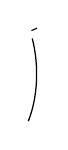
\begin{tikzpicture}[x=1mm,y=1mm]
\draw[line width=.45pt] (.1,5.5) ..controls(1,2)and(.8,-2)..(-.4,-5);
\draw[line width=.4pt] (0,6.5)--(.7,6.8);
\end{tikzpicture}}

\Unclear{GELFAND-P000282}{bottom-right-mark}{Внизу справа изогнутый вертикальный штрих и отдельная короткая помета над ним: ) / 1. Чтение не установлено.}
\end{GelfandAdjacentEvidence}




\Needspace{7\baselineskip}
\SourcePage{GELFAND-P000283}{unlabelled}
\textbf{15.9.69г.}

\underline{\underline{Б. Вайнберг}} о рез. Хёрмандера. (см. сем. Вишика). про особенности фунд. реш.

Общее реш. однор. ур-я: (однор. многочлен)

\begin{equation*}\int_{P(\xi)=0}f[(x,\xi)]A(\xi)\,d\xi\qquad\text{(Боровиков)}\end{equation*}

$f,A$ — произв. функции.

Особенности в случае однор. описаны Боровиковым.

Например:

\begin{GelfandAdjacentEvidence}{GELFAND-P000283}{1}
\begin{equation*}\int_{P(\xi)=0}\frac{(x\cdot\xi)^\lambda}{\Gamma(\lambda+1)}A(\xi)\,d\xi\end{equation*}

\Unclear{GELFAND-P000283}{borovikov-numerator}{Между $x$ и $\xi$ короткий пересечённый штрих: точка / плюс / запятая. Скобки и верхний индекс $\lambda$ видны; вариант с точкой не установлен.}
\end{GelfandAdjacentEvidence}


— предл. Боровикова.

\begin{center}\GelfandFitDiagram{\begin{tikzpicture}
\node (f) {$R_0^+$ (станд. фунд. реш.)};
\draw ([xshift=-4pt,yshift=5pt]f.north west)--([xshift=-4pt,yshift=-3pt]f.south west)--([xshift=4pt,yshift=-3pt]f.south east)--([xshift=4pt,yshift=5pt]f.north east);
\end{tikzpicture}}\end{center}





Грушин:

\begin{equation*}\sum_j\int\frac{\alpha_j(\xi)e^{i(x,\xi)}}{P(\xi)\pm i0}\,d\xi\end{equation*}

$\alpha_j$ — разл. ед. на сфере.





\underline{Решена проблема Бернштейна.}

\begin{GelfandAdjacentEvidence}{GELFAND-P000283}{2}
\begin{equation*}\left\{\begin{gathered}
z=f(x_1,\ldots,x_{n-1})\text{ — миним. пов.}\\
(x\text{-любые})\ \Longrightarrow\ \text{она плоск.}
\end{gathered}\right\}\end{equation*}

\Unclear{GELFAND-P000283}{graph-variable-index}{Последний индекс переменной: $n-1$ / $n+1$; короткие штрихи сливаются. Чтение не установлено.}
\end{GelfandAdjacentEvidence}


верно при $n\leq8$; при $n\geq9$ \underline{\underline{неверно}}.

\GelfandFitDiagram{\begin{tikzpicture}[baseline=(n.base)]\node[inner sep=0pt](n){Де Джиорджи};\draw[dashed]([yshift=-2pt]n.south west)--([yshift=-2pt]n.south east);\end{tikzpicture}}, \GelfandFitDiagram{\begin{tikzpicture}[baseline=(n.base)]\node[inner sep=0pt](n){Саймонс};\draw[dashed]([yshift=-2pt]n.south west)--([yshift=-2pt]n.south east);\end{tikzpicture}} и \GelfandFitDiagram{\begin{tikzpicture}[baseline=(n.base)]\node[inner sep=0pt](n){Бомбьери};\draw[dashed]([yshift=-2pt]n.south west)--([yshift=-2pt]n.south east);\end{tikzpicture}}.

\GelfandFitDiagram{\begin{tikzpicture}[baseline=(k.base)]
\node[inner sep=0pt](k){Каздан и Бернштейн.};
\draw[<-]([yshift=-1pt]k.south west)--([yshift=-1pt]k.south east);
\draw([yshift=-3pt]k.south west)--([yshift=-3pt]k.south east);
\end{tikzpicture}}

\begin{GelfandAdjacentEvidence}{GELFAND-P000283}{3}
Сходимость спектра при расширении областей.





\SourceFigure{GELFAND-P000283}{nested-domains}{\par\smallskip\centering{\color{black}\GelfandFitDiagram{\begin{minipage}{68mm}\raggedright \GelfandFitDiagram{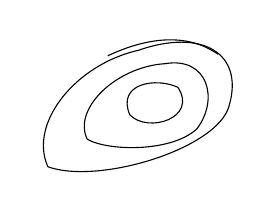
\begin{tikzpicture}
\draw (0,0) .. controls (-0.25,0.55) and (0.35,1.30) .. (1.15,1.48)
 .. controls (1.95,1.76) and (2.50,1.45) .. (2.30,0.77)
 .. controls (2.15,0.23) and (0.65,-0.23) .. (0,0);
\draw (0.50,0.35) .. controls (0.31,0.73) and (0.86,1.27) .. (1.49,1.31)
 .. controls (2.03,1.40) and (2.18,0.86) .. (1.89,0.48)
 .. controls (1.56,0.18) and (0.76,0.20) .. (0.50,0.35);
\draw (1.04,0.66) .. controls (0.87,1.06) and (1.37,1.14) .. (1.65,1.01)
 .. controls (1.91,0.62) and (1.27,0.42) .. (1.04,0.66);
\draw (0.76,1.41) .. controls (1.25,1.64) and (1.76,1.71) .. (2.16,1.43);
\end{tikzpicture}}\end{minipage}}}\par\smallskip }
\end{GelfandAdjacentEvidence}


$A$ — самосопр. опер. на мн-зии $X$.

$\Lambda\subset R$.

[Под $\Lambda$:] \uwave{отрезок}.

\uwave{В $E_\Lambda$ плотны содержащиеся там непрерывные ф-и.}

(требуется) — так для эл. опер.

$x_0\longrightarrow$ мера Планшереля на спектре $A$.

\begin{GelfandAdjacentEvidence}{GELFAND-P000283}{4}
\begin{equation*}M_{x_0}(\Lambda)=
\max_{\substack{f\text{-непр. в }E_\lambda,\ \|f\|=1\\
\text{(по всему }X\text{)}}}|f(x_0)|^2.\end{equation*}

\Unclear{GELFAND-P000283}{spectral-subscript}{Под $\max$: $E_\lambda$; возможно, $E_\Lambda$. Выше обозначения $E_\Lambda$ и $M_{x_0}(\Lambda)$; регистр не унифицирован.}
\end{GelfandAdjacentEvidence}


[Справа:] Это мера (быть может, беск.)



\Needspace{7\baselineskip}
\SourcePage{GELFAND-P000284}{53}
$K_\Lambda(x,y)$ — ядро $E_\Lambda$.

\begin{flushright}\GelfandFitDiagram{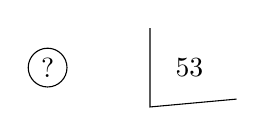
\begin{tikzpicture}[x=1mm,y=1mm]
\node[draw,circle,inner sep=2pt](q)at(-18,0){?};
\node at(0,0){$53$};
\draw(-5,5)--(-5,-5)--(6,-4);
\end{tikzpicture}}\end{flushright}
\begin{center}\GelfandFitDiagram{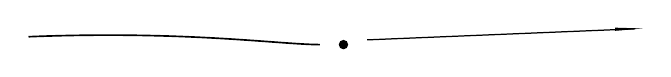
\begin{tikzpicture}[x=1mm,y=1mm]
\draw[line width=.6pt](-40,0)..controls(-20,.8)and(-8,-1)..(-3,-1);
\fill(0,-1)circle[radius=.6mm];
\draw[line width=.45pt](3,-.4)--(37,1);
\fill(34.5,.75)--(38,1.05)--(34.5,1.15)--cycle;
\end{tikzpicture}}\end{center}





\underline{Каздан.} М. Артин в сем. Бурбаки.

\begin{equation*}f_i(x_1,\ldots,x_n)=0,\qquad1\leq i\leq k.\end{equation*}

$f_i$ — сход. степ. ряды.

\begin{GelfandAdjacentEvidence}{GELFAND-P000284}{1}
Когда сущ. реш. $\psi_j(t_1,\ldots,t_\tau)$

\Unclear{GELFAND-P000284}{artin-solution-parameters}{Буква функции: $\psi$ / $Y$; последний индекс: $\tau$ / $r$. Чтение не установлено.}
\end{GelfandAdjacentEvidence}


\underline{Ответ:} тогда и только тогда, когда есть реш. в форм. степ. рядах.

(сколь угодно близко к формальному)

[Под скобкой:] достраивается

\begin{center}\GelfandFitDiagram{\begin{tikzpicture}[x=1mm,y=1mm]
\draw[line width=.55pt](-20,0)--(-3,0);
\fill(0,0)circle[radius=.6mm];
\draw[line width=.55pt](3,0)--(20,0);
\end{tikzpicture}}\end{center}

\textbf{22.9.69г.}

\begin{GelfandAdjacentEvidence}{GELFAND-P000284}{2}
\underline{Фикера} \underline{об} \underline{одностор.} \underline{гран.} \underline{задачах.}





\SourceFigure{GELFAND-P000284}{elastic-body}{\par\smallskip\centering{\color{black}\GelfandFitDiagram{\begin{minipage}{68mm}\raggedright \GelfandFitDiagram{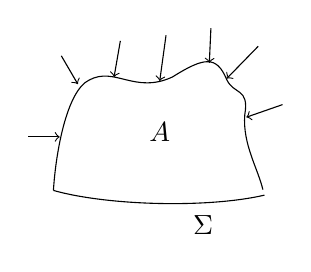
\begin{tikzpicture}
\draw (0,0.08) .. controls (0.03,0.57) and (0.17,1.34) .. (0.45,1.48)
 .. controls (0.78,1.66) and (1.03,1.30) .. (1.51,1.52)
 .. controls (1.91,1.77) and (2.07,1.80) .. (2.20,1.49)
 .. controls (2.29,1.29) and (2.49,1.39) .. (2.43,1.04)
 .. controls (2.40,0.67) and (2.60,0.35) .. (2.66,0.09);
\draw (0,0.08) .. controls (0.67,-0.11) and (1.94,-0.15) .. (2.68,0.02);
\draw[->] (-0.32,0.76) -- (0.08,0.76);
\draw[->] (0.10,1.79) -- (0.31,1.43);
\draw[->] (0.85,1.98) -- (0.77,1.52);
\draw[->] (1.43,2.05) -- (1.35,1.47);
\draw[->] (2.00,2.14) -- (1.98,1.70);
\draw[->] (2.60,1.91) -- (2.20,1.50);
\draw[->] (2.91,1.17) -- (2.45,1.01);
\node at (1.35,0.82) {$A$};
\node at (1.90,-0.36) {$\Sigma$};
\end{tikzpicture}}\end{minipage}}}\par\smallskip }
\end{GelfandAdjacentEvidence}


Эластичн. тело на пов. $\Sigma$ жёсткой и без трения.

И тензор напр. $\equiv0$.

$A$ — естеств. объём тела.

На своб. части границы сила \GelfandFitDiagram{\begin{tikzpicture}[baseline=(p.base)]
\node(p)at(0,0){$\varphi$};
\draw(-.35,-.25)..controls(-.35,-.45)and(.15,-.45)..(.4,-.25);
\node at(0,-.7){плотность};
\end{tikzpicture}} на $\partial A-\Sigma=\Sigma^*$.





Внутри тоже нек-рые силы $f$ — объёмные.

Пусть тело перех. в полож. равн.

\begin{GelfandAdjacentEvidence}{GELFAND-P000284}{3}
Оно может отойти от $\Sigma$.





\Unclear{GELFAND-P000284}{detachment-figure}{Слева касание видно. Справа наложенные штрихи и узкая светлая полоса; точное касание или зазор и протяжённость контакта не установлены. Подписей и стрелок нет.\par\smallskip\centering{\color{black}\GelfandFitDiagram{\begin{minipage}{68mm}\raggedright \GelfandFitDiagram{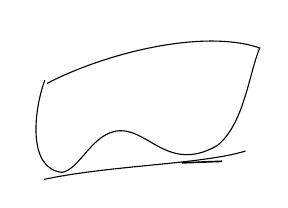
\begin{tikzpicture}
\draw (.14,1.16)..controls(.85,1.53)and(2.10,1.86)..(2.84,1.61)
 ..controls(2.70,1.27)and(2.64,.64)..(2.30,.37)
 ..controls(1.66,.00)and(1.40,.64)..(1.00,.55)
 ..controls(.70,.49)and(.54,.06)..(.33,.03)
 ..controls(-.10,.07)and(-.04,.78)..(.11,1.20);
\draw (.10,-.06)..controls(.94,.12)and(2.10,.13)..(2.66,.30);
\draw[line width=.6pt](1.85,.15)--(2.36,.17);
\end{tikzpicture}}\end{minipage}}}\par\smallskip }
\end{GelfandAdjacentEvidence}


Это аналит. задача (постановка A. Signorini, 1959)

$\sigma_{ik}$ — тензор напряжений.

Внутри тела

[Зачёркнуто:] \GelfandFitDiagram{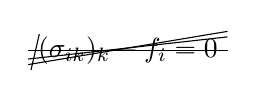
\begin{tikzpicture}[baseline=(c.base)]
\node(c){$(\sigma_{ik})_k-f_i=0$};
\draw(c.west)--(c.east);
\draw([yshift=-3pt]c.west)--([yshift=5pt]c.east);
\draw([yshift=-5pt]c.west)--([yshift=7pt]c.east);
\draw([xshift=1pt,yshift=-7pt]c.west)--([xshift=4pt,yshift=6pt]c.west);
\end{tikzpicture}}





[Справа написано:]

\begin{equation*}\sigma_{ik/k}-f_i=0.\end{equation*}

$(\operatorname{div}\sigma=f)$.

\begin{equation*}\sigma_{ik}\nu_k-\varphi_i=0.\end{equation*}

— гран. условия.

\begin{GelfandAdjacentEvidence}{GELFAND-P000284}{4}
($\nu$ — вект. нормали)

\Unclear{GELFAND-P000284}{normal-letter}{Знак нормали в формуле и подписи имеет вид $V$ / $\nu$; выбор буквы по одному начертанию не установлен.}
\end{GelfandAdjacentEvidence}




\Needspace{7\baselineskip}
\SourcePage{GELFAND-P000285}{unlabelled}
\GelfandFitDiagram{\begin{tikzpicture}[baseline=(s.base)]
\node(s){\underline{На $\Sigma$.}};
\draw([xshift=-2pt]s.north west)--([xshift=-2pt,yshift=-2pt]s.south west)--([xshift=2pt,yshift=-2pt]s.south east)--([xshift=2pt]s.north east);
\end{tikzpicture}}

$u_i$ — вектор смещения.

\begin{GelfandAdjacentEvidence}{GELFAND-P000285}{1}
\begin{center}\GelfandFitDiagram{\begin{tikzpicture}[x=1mm,y=1mm]
\node at(-29,18){Условие};
\node at(4,18){$u_i\nu_i=0\quad(\text{на }\Sigma)$};
\node at(-19,3){Норм. реакция};
\node at(29,3){$\sigma_{ik}\nu_i\nu_k\geq0$};
\node at(29,-11){$\sigma_{ik}\nu_i\tau_k=0$};
\node[anchor=west,inner sep=0pt] at(62,-11){$\text{— танг. комп.}$};
\draw(-18,26)--(-18,11)--(9,8)--(9,-20)--(58,-20)--(58,-8);
\end{tikzpicture}}\end{center}

\Unclear{GELFAND-P000285}{contact-framing-normal}{Условия объединены ступенчатой открытой линией. Знак нормали имеет вид $\nu$ / $V$; начертание само по себе не устанавливает букву.}
\end{GelfandAdjacentEvidence}


В точке своб. поверхн:

\begin{equation*}\begin{cases}
u_i\nu_i>0,\\
\sigma_{ik}\nu_i\nu_k=0,\\
\sigma_{ik}\nu_i\tau_k=0.
\end{cases}\end{equation*}

\textbf{Но} неизвестно, где что.

Не учли ещё, что упругое тело.

\begin{center}\GelfandFitDiagram{\begin{tikzpicture}
\node(p)at(0,0){$\underline{\underline{W(x,\varepsilon)}}$};
\node at(0,-.55){потенциал};
\end{tikzpicture}}\end{center}

\begin{equation*}\varepsilon=\{\varepsilon_{ik}\}\qquad\varepsilon_{ik}=2^{-1}(u_{i/k}+u_{k/i})\end{equation*}

\begin{center}Тенз. деформации.\end{center}





Связь:

\begin{equation*}\sigma_{ik}+W_{\varepsilon_{ik}}=0\qquad\text{на }A.\end{equation*}

Пробл. сущ. и единств.

\begin{equation*}\begin{aligned}
I(u)={}&\int_A W[x,\varepsilon(u)]\,dx\\
&-\underbrace{\int_A f_i u_i\,dx}_{\text{работа }f}
-\underbrace{\int_\Sigma\varphi_i u_i\,d\Sigma}_{\text{работа }\varphi}.
\end{aligned}\end{equation*}

\begin{GelfandAdjacentEvidence}{GELFAND-P000285}{2}
(Энергия суммарная)

\Unclear{GELFAND-P000285}{energy-boundary-domain}{В первом поверхностном интеграле написано $\Sigma$, без звёздочки.}
\end{GelfandAdjacentEvidence}


\begin{GelfandAdjacentEvidence}{GELFAND-P000285}{3}
\uwave{В классе допуст. смещений $\mathcal W_\Sigma$.}

\Unclear{GELFAND-P000285}{admissible-class-letter}{Жирно наведённая буква: $\mathcal W_\Sigma$ / $\mathcal U_\Sigma$; не унифицирована с нижним обозначением модельного класса.}
\end{GelfandAdjacentEvidence}


Если сущ. минимум в $C^1(\Sigma)$, то он решение.

\begin{GelfandAdjacentEvidence}{GELFAND-P000285}{4}
обратно, решение — $\min$.

\Unclear{GELFAND-P000285}{regularity-domain}{Написано $C^1(\Sigma)$; над $\Sigma$ нет черты.}
\end{GelfandAdjacentEvidence}


Но: в этом классе \GelfandFitDiagram{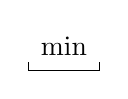
\begin{tikzpicture}[baseline=(m.base)]
\node(m){$\min$};
\draw([xshift=-1pt,yshift=1pt]m.south west)--([xshift=-1pt,yshift=-2pt]m.south west)--([xshift=1pt,yshift=-2pt]m.south east)--([xshift=1pt,yshift=1pt]m.south east);
\end{tikzpicture}} не сущ.





\begin{center}\GelfandFitDiagram{\begin{tikzpicture}[x=1mm,y=1mm]
\draw[line width=.55pt](-20,0)--(-3,0);
\fill(0,0)circle[radius=.35mm];
\draw[line width=.55pt](3,0)--(20,0);
\end{tikzpicture}}\end{center}

\begin{equation*}\begin{aligned}
I(u)={}&\frac12\int_A a_{nk}(x)u_{/n}u_{/k}\,dx\\
&-\int_A fu\,dx-\int_{\Sigma^*}\varphi u\,d\sigma.
\end{aligned}\end{equation*}

\begin{equation*}a_{nk}(x)\mu_n\mu_k\geq\rho_0\mu_n\mu_n.\end{equation*}

\begin{equation*}\mathcal U_\Sigma:\quad u|_\Sigma\geq0.\end{equation*}

\begin{GelfandAdjacentEvidence}{GELFAND-P000285}{5}
(Модельная задача)





\Unclear{GELFAND-P000285}{boundary-partition-figure}{Верхняя дуга: $\Sigma^*$; нижняя слева: $\Sigma$. Две кольцевые отметки стыков; левая перечерчена, с косым штрихом. Его назначение и направление обхода не установлены.\par\smallskip\centering{\color{black}\GelfandFitDiagram{\begin{minipage}{68mm}\raggedright \GelfandFitDiagram{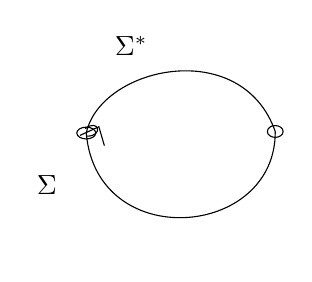
\begin{tikzpicture}
\draw(0,0)..controls(.18,.84)and(1.97,1.24)..(2.40,.02);
\draw(2.40,.02)..controls(2.41,-1.34)and(.13,-1.53)..(0,0);
\draw(0,0)ellipse[x radius=.12,y radius=.075];
\draw(2.40,.02)ellipse[x radius=.10,y radius=.075];
\draw(-.015,.055)..controls(.16,.19)and(.22,-.04)..(.01,-.04);
\draw(-.08,-.03)--(.16,.08)--(.23,-.16);
\node at(.57,1.10){$\Sigma^*$};
\node at(-.50,-.66){$\Sigma$};
\end{tikzpicture}}\end{minipage}}}\par\smallskip }
\end{GelfandAdjacentEvidence}




\Needspace{7\baselineskip}
\SourcePage{GELFAND-P000286}{54}
Отсюда получ. зад.

\begin{center}\GelfandFitDiagram{\begin{tikzpicture}
\node(b){$u=0,\quad a\dfrac{\partial u}{\partial\lambda}\geq0$};
\draw[line width=.6pt](b.north west)--(b.north east)--(b.south east)--(b.south west)--cycle;
\draw([xshift=-2pt]b.west)..controls(b.north west)and(b.north east)..([xshift=2pt]b.east)..controls(b.south east)and(b.south west)..([xshift=-2pt]b.west);
\draw([yshift=-5pt]b.south west)--([yshift=-5pt]b.south east);
\draw([xshift=4pt,yshift=-1pt]b.south west)--([xshift=10pt,yshift=-5pt]b.south west);
\draw([xshift=16pt,yshift=-1pt]b.south west)--([xshift=22pt,yshift=-5pt]b.south west);
\draw([xshift=28pt,yshift=-1pt]b.south west)--([xshift=34pt,yshift=-5pt]b.south west);
\draw([xshift=40pt,yshift=-1pt]b.south west)--([xshift=46pt,yshift=-5pt]b.south west);
\draw([xshift=52pt,yshift=-1pt]b.south west)--([xshift=58pt,yshift=-5pt]b.south west);
\draw([xshift=64pt,yshift=-1pt]b.south west)--([xshift=70pt,yshift=-5pt]b.south west);
\draw([xshift=76pt,yshift=-1pt]b.south west)--([xshift=82pt,yshift=-5pt]b.south west);
\draw([xshift=88pt,yshift=-1pt]b.south west)--([xshift=94pt,yshift=-5pt]b.south west);
\end{tikzpicture}}
\quad\text{или}\quad
$\begin{cases}u>0,\\a\dfrac{\partial u}{\partial\lambda}=0.\end{cases}$
\end{center}

\begin{flushright}\GelfandFitDiagram{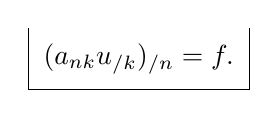
\begin{tikzpicture}[baseline=(f.base)]
\node(f){$(a_{nk}u_{/k})_{/n}=f.$};
\draw([xshift=-2pt,yshift=2pt]f.north west)--([xshift=-2pt,yshift=-2pt]f.south west)--([xshift=2pt,yshift=-2pt]f.south east)--([xshift=2pt,yshift=2pt]f.north east);
\end{tikzpicture}}\quad\GelfandFitDiagram{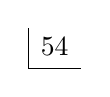
\begin{tikzpicture}\node(p){$54$};\draw([xshift=-1pt]p.north west)--([xshift=-1pt,yshift=-1pt]p.south west)--([xshift=1pt,yshift=-1pt]p.south east);\end{tikzpicture}}\end{flushright}





Необходимо:

\begin{GelfandAdjacentEvidence}{GELFAND-P000286}{1}
\begin{equation*}\int_A f\,dx+\int_{\Sigma^*}\varphi\,d\Sigma\leq0.\end{equation*}

\Unclear{GELFAND-P000286}{first-integral-differential}{Дифференциал первого интеграла: $dx$ / $d\Sigma$; возможно, $\Sigma$ исправлена на $x$. Штрихи наложены друг на друга.}
\end{GelfandAdjacentEvidence}
\begin{GelfandAdjacentEvidence}{GELFAND-P000286}{2}


\Unclear{GELFAND-P000286}{first-integral-domain-overwrite}{Итоговое $A$ под первым интегралом наведено поверх прежних штрихов. Возможная прежняя $\Sigma$ не установлена.}
\end{GelfandAdjacentEvidence}


Пусть $f\leq0$ на $A$ и $\varphi<0$ на $\Sigma^*$.

По принц. $\min$  $u$ не может иметь мин. в $A$.

Не имеет реш. в $\underline{\underline{C^1(\bar A)}}$.

\GelfandFitDiagram{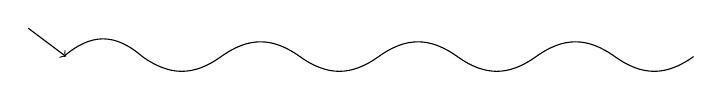
\begin{tikzpicture}
\draw[->](-.45,.36)--(.03,0);
\draw(0,0)..controls(.35,.30)and(.65,.30)..(1,0)..controls(1.35,-.25)and(1.65,-.25)..(2,0)
 ..controls(2.35,.25)and(2.65,.25)..(3,0)..controls(3.35,-.25)and(3.65,-.25)..(4,0)
 ..controls(4.35,.25)and(4.65,.25)..(5,0)..controls(5.35,-.25)and(5.65,-.25)..(6,0)
 ..controls(6.35,.25)and(6.65,.25)..(7,0)..controls(7.35,-.25)and(7.65,-.25)..(8,0);
\end{tikzpicture}}

(выв. из ф-лы Грина)

\uwave{сразу противоречие — получ. разрыв производной.}





\GelfandFitDiagram{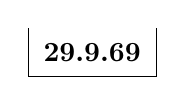
\begin{tikzpicture}[baseline=(f.base)]
\node(f){\textbf{29.9.69}};
\draw([xshift=-2pt,yshift=2pt]f.north west)--([xshift=-2pt,yshift=-2pt]f.south west)--([xshift=2pt,yshift=-2pt]f.south east)--([xshift=2pt,yshift=2pt]f.north east);
\end{tikzpicture}}

\underline{Каздан} \uwave{Формулировка} рез. \uwave{М. Артина}. (1968).





\begin{GelfandAdjacentEvidence}{GELFAND-P000286}{3}
(в СССР независ. Покорний и Рыбкин)

\Unclear{GELFAND-P000286}{pokorny-surname}{Первая фамилия: Покорний / Покорный; соединённое окончание не устанавливает и или ы.}
\end{GelfandAdjacentEvidence}


УМН, т. 15, $N=4$ (1960) стр. 169

и Меламед

Сиб. мат. журнал

\begin{equation*}f_i(x_1,\ldots,x_k)=0,\qquad1\leq i\leq n.\end{equation*}

набор. сход. степ. рядов (в окр. 0

Пытаемся найти

\begin{center}\GelfandFitDiagram{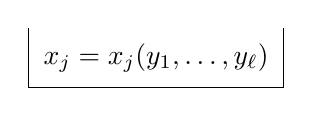
\begin{tikzpicture}[baseline=(f.base)]
\node(f){$x_j=x_j(y_1,\ldots,y_\ell)$};
\draw([xshift=-2pt,yshift=2pt]f.north west)--([xshift=-2pt,yshift=-2pt]f.south west)--([xshift=2pt,yshift=-2pt]f.south east)--([xshift=2pt,yshift=2pt]f.north east);
\end{tikzpicture}}\quad\GelfandFitDiagram{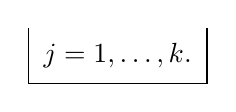
\begin{tikzpicture}[baseline=(f.base)]
\node(f){$j=1,\ldots,k.$};
\draw([xshift=-2pt,yshift=2pt]f.north west)--([xshift=-2pt,yshift=-2pt]f.south west)--([xshift=2pt,yshift=-2pt]f.south east)--([xshift=2pt,yshift=2pt]f.north east);
\end{tikzpicture}}\end{center}

чтобы рав-ва вып. при подстановке.

\underline{Достат. найти такие ф-и в форм. степ. рядах.}

\noindent\begin{tabular}{@{}p{.44\linewidth}|p{.48\linewidth}@{}}
\underline{Пример.}
\begin{equation*}x_1^2-x_2^3=0\qquad\begin{aligned}x_1&=y^3,\\x_2&=y^2.\end{aligned}\end{equation*}
& Тогда найд. реш. в аналит. ф-ях, сколь угодно близкое. (с люб. числом производных)\\\hline
\end{tabular}





зад. делается индукцией по числу $x_j$.

и более сложн. инд.

\underline{Переформул.}

Это ур-я аналит. мн-ва и 2 кольца

\begin{align*}
A&=C\{y_1,\ldots,y_\ell\}&&\text{сход. ряды.}\\
B&=C[[y_1,\ldots,y_\ell]]&&\text{форм. ряды.}
\end{align*}

Если \GelfandFitDiagram{\begin{tikzpicture}[baseline=-.5ex]
\node(i){у мн-зия};
\draw[rounded corners=3pt]([xshift=-3pt,yshift=2pt]i.north west)--([xshift=3pt,yshift=2pt]i.north east)--([xshift=3pt,yshift=-2pt]i.south east)--([xshift=10pt,yshift=-2pt]i.south west)--([xshift=3pt,yshift=-9pt]i.south west)--([xshift=1pt,yshift=-2pt]i.south west)--([xshift=-3pt,yshift=-2pt]i.south west)--cycle;
\end{tikzpicture}} есть точка со знач. в $B$, то есть точка и со знач. в $A$.







\Needspace{7\baselineskip}
\SourcePage{GELFAND-P000287}{unlabelled}
Индукция и по связн. компонентам. (\underline{\underline{числу их}})

Непривод. --- подкусок имеет меньшую размерность.

1) \uwave{Если для неприв. $\underset{\text{(данной разм.)}}{\text{мн-зий}}$ док., то и $\underset{\text{(данн. разм.)}}{\text{всегда док.}}$}





\begin{GelfandAdjacentEvidence}{GELFAND-P000287}{1}
Выб. ур-я, леж. в идеале, \textbf{[зачёркнуто: ?]} соотв. этой компоненте.

\Unclear{GELFAND-P000287}{upper-cancelled-word}{Между «идеале,» и «соотв.» густо зачёркнуто слово. Начальный штрих похож на «к»; полное чтение не установлено.}
\end{GelfandAdjacentEvidence}


\begin{GelfandAdjacentEvidence}{GELFAND-P000287}{2}
\uwave{Добавл. ур-ей.} Рассм. простой идеал.





\SourceFigure{GELFAND-P000287}{crossing-sketch}{\par\smallskip\centering{\color{black}\GelfandFitDiagram{\begin{minipage}{68mm}\raggedright \GelfandFitDiagram{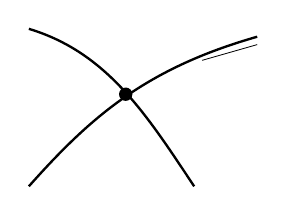
\begin{tikzpicture}[x=1mm,y=1mm]
\draw[line width=.85pt] (0,0) ..controls(8,9)and(15,15)..(29,19);
\draw[line width=.85pt] (0,20) ..controls(10,17)and(15,9)..(21,0);
\draw[line width=.3pt] (22,16)--(29,18);
\fill (12.3,11.7) circle[radius=.85mm];
\end{tikzpicture}}\end{minipage}}}\par\smallskip }
\end{GelfandAdjacentEvidence}


\begin{GelfandAdjacentEvidence}{GELFAND-P000287}{3}
$\mathcal J=($\uwave{Пересеч. простых}$)$.

\Unclear{GELFAND-P000287}{ideal-letter}{Знак перед равенством имеет длинный нижний крюк: $\mathcal J$ / $\mathcal I$; буквенное обозначение не установлено.}
\end{GelfandAdjacentEvidence}


Получ. 2 сист. ур-й. $\forall$ решение удовл. \underline{\underline{одной}} \underline{\underline{из}} этих систем.

\begin{GelfandAdjacentEvidence}{GELFAND-P000287}{4}
(Если геом. точка леж. на \textbf{[зачёркнуто: ?]} мн-зии, то она лежит на одной из компонент.)

\Unclear{GELFAND-P000287}{middle-cancelled-word}{Между «на» и «мн-зии» короткое слово или начало слова перекрыто несколькими линиями; достоверная последовательность букв не установлена.}
\end{GelfandAdjacentEvidence}


\begin{GelfandAdjacentEvidence}{GELFAND-P000287}{5}
\textbf{[На левом поле зачёркнутый знак: ?]}

\Unclear{GELFAND-P000287}{left-cancelled-mark}{Компактный многократно перечёркнутый знак с петлями. Буква, номер либо нетекстовая помета не установлены.}
\end{GelfandAdjacentEvidence}


Остальное --- в следующий раз.

\begin{GelfandAdjacentEvidence}{GELFAND-P000287}{940}
\underline{\underline{Л. Фаддеев.}}

\underline{О результ. одного вычисл. эксперимента}, \textbf{[зачёркнуто: ?]} \underline{им. отн. к прогр. Кириллова}

\hfill\underline{опис. предст.}





\Unclear{GELFAND-P000287}{title-cancelled-word}{После «эксперимента,» перед «им. отн.» отменено слово. Начало похоже на «ре»; варианты «реал.» / «рез...» не установлены.}
\end{GelfandAdjacentEvidence}


Представление --- квантование класс. механики.

Примеры и пробл. о правилах квантования.

\begin{GelfandAdjacentEvidence}{GELFAND-P000287}{7}
$M_{2n}$ --- симпл. мн-зие, обл.? $\Omega$ --- 2-формой (невырожд.).\qquad $\Omega=d\omega$.

\Unclear{GELFAND-P000287}{form-abbreviation}{Сокращение после «симпл. мн-зие»: «обл.» / «обал.»; промежуточный штрих неоднозначен. Полное слово не установлено.}
\end{GelfandAdjacentEvidence}


$d\mu=\Omega^n$ --- мера.

\begin{GelfandAdjacentEvidence}{GELFAND-P000287}{8}
\begin{equation*}f\longrightarrow X_f\qquad (\text{по ф-ии поле})\end{equation*}





\SourceFigure{GELFAND-P000287}{hamiltonian-definition-frame}{\par\smallskip\centering{\color{black}\GelfandFitDiagram{\begin{minipage}{68mm}\raggedright \GelfandFitDiagram{\begin{tikzpicture}[baseline=(formula.base)]
\node[inner sep=2pt] (formula) {$\Omega(X_f,Y)=Yf$};
\draw[line width=.85pt] ([xshift=-2mm,yshift=3mm]formula.west)--([xshift=-2mm,yshift=-4mm]formula.south west)--([xshift=2mm,yshift=-4mm]formula.south east)--([xshift=2mm,yshift=3mm]formula.east);
\draw[line width=.5pt] ([xshift=-2mm,yshift=-2.5mm]formula.south west)--([xshift=2mm,yshift=-2.5mm]formula.south east);
\path (formula.south west)++(-2mm,-4mm)coordinate(hatchleft);
\path (formula.south east)++(2mm,-4mm)coordinate(hatchright);
\foreach \k in {0,.05,...,.95}{\draw[line width=.25pt] ($(hatchleft)!\k!(hatchright)$)--++(1.2mm,1.5mm);}
\end{tikzpicture}}\end{minipage}}}\par\smallskip }
\end{GelfandAdjacentEvidence}


Гамильтоновы поля $X_f$ образ. алгебру Ли

\begin{equation*}[X_f,X_g]=X_{\{f,g\}},\end{equation*}

где $\{f,g\}$ --- скобки Пуассона (она этим определяется).

Опер. $X_f$ антисимм. в $L^2$ с мерой $d\mu=\Omega^n$. (Она сохр. по теор. Лиувилля.)

Элем. алгебры Ли $X_f\longrightarrow$ отвечает опер. в $L^2$.

\underline{1951} Ван Хов нашёл 1-пар. сем-во представлений.

\begin{equation*}Z_f=X_f+\alpha\bigl(\omega(X_f)-f\bigr)\end{equation*}



\Needspace{7\baselineskip}
\SourcePage{GELFAND-P000288}{55}
\hfill\GelfandFitDiagram{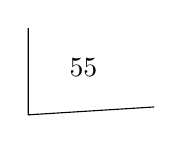
\begin{tikzpicture}[x=1mm,y=1mm]\draw(0,11)--(0,0)--(16,1);\node[inner sep=1pt]at(7,6){$55$};\end{tikzpicture}}

Тогда вып. условие представления

\begin{equation*}\omega(X_f)-f=\ell_f\end{equation*}

\begin{GelfandAdjacentEvidence}{GELFAND-P000288}{950}
\underline{Утвержд. Ван-Хова:} Это снова предст., не эквив. ни при одном $\alpha$

\begin{equation*}[Z_f,Z_g]=Z_{\{f,g\}}\end{equation*}\end{GelfandAdjacentEvidence}

Но это ещё не переход к квантовой механике, т. к. пока всё в пр-ве \underline{всех переменных}, а не половины их.

Рассм. теперь $SO(3)$ с ест. предст. в $\mathbb R^3$. На орбитах $(S^2)$ естеств. компл. структура.

\begin{GelfandAdjacentEvidence}{GELFAND-P000288}{1}
Результат вычисления $Z_f$, когда $X_f$ --- генер. группы вращ.





\SourceFigure{GELFAND-P000288}{cancelled-generators}{\par\smallskip\centering{\color{black}\GelfandFitDiagram{\begin{minipage}{68mm}\raggedright \GelfandFitDiagram{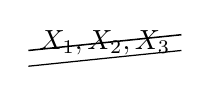
\begin{tikzpicture}[baseline=(cancelled.base)]
\node[inner sep=1pt](cancelled){$X_1,X_2,X_3$};
\draw[line width=.55pt]([xshift=-1mm,yshift=-1mm]cancelled.west)--([xshift=1mm,yshift=1mm]cancelled.east);
\draw[line width=.45pt]([xshift=-1mm,yshift=-3mm]cancelled.west)--([xshift=1mm,yshift=-1mm]cancelled.east);
\end{tikzpicture}}\end{minipage}}}\par\smallskip }
\end{GelfandAdjacentEvidence}


\begin{equation*}x_1^2+x_2^2+x_3^2=a^2\quad\text{--- орбита}\end{equation*}

Функции $x_1,x_2,x_3$. Соотв. опер. Ван-Хова:

\begin{center}\GelfandFitDiagram{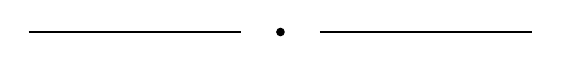
\begin{tikzpicture}[x=1mm,y=1mm]\draw[line width=.6pt](-32,0)--(-5,0);\fill(0,0)circle[radius=.55mm];\draw[line width=.6pt](5,0)--(32,0);\end{tikzpicture}}\end{center}

\begin{GelfandAdjacentEvidence}{GELFAND-P000288}{2}
\underline{\underline{Зад. квантования.}}





\SourceFigure{GELFAND-P000288}{phase-plane}{\par\smallskip\centering{\color{black}\GelfandFitDiagram{\begin{minipage}{68mm}\raggedright \GelfandFitDiagram{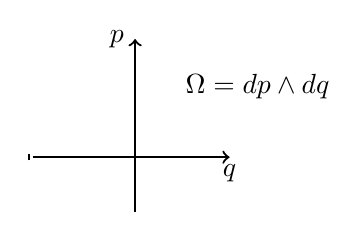
\begin{tikzpicture}[x=1mm,y=1mm]
\draw[->,line width=.8pt](-13,0)--(12,0);
\draw[->,line width=.8pt](0,-7)--(0,15);
\draw[line width=.8pt](-13.5,-.4)--(-13.5,.4);
\node[anchor=north,inner sep=1pt]at(12,-.5){$q$};
\node[anchor=east,inner sep=1pt]at(-1,15){$p$};
\node[anchor=west,inner sep=1pt]at(6,9){$\Omega=dp\wedge dq$};
\end{tikzpicture}}\end{minipage}}}\par\smallskip }
\end{GelfandAdjacentEvidence}


Гамильтониан $f=\dfrac{p^2}{2m}$ (своб. частица).

Надо ей сопост. оператор.

\begin{center}\GelfandFitDiagram{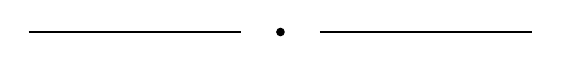
\begin{tikzpicture}[x=1mm,y=1mm]\draw[line width=.6pt](-32,0)--(-5,0);\fill(0,0)circle[radius=.55mm];\draw[line width=.6pt](5,0)--(32,0);\end{tikzpicture}}\end{center}

\begin{GelfandAdjacentEvidence}{GELFAND-P000288}{3}
$f=x_1$.





\Unclear{GELFAND-P000288}{stereographic-diagram}{Округлый контур касается почти горизонтальной линии; из верхней области идут четыре наклонных штриха. Крайний правый заканчивается выше нижней линии. Слева небольшой крючок: стрелка влево / неровность линии; направление и точные соединения верхних штрихов не установлены. Подписей нет.\par\smallskip\centering{\color{black}\GelfandFitDiagram{\begin{minipage}{68mm}\raggedright \GelfandFitDiagram{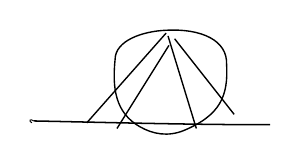
\begin{tikzpicture}[x=.12mm,y=.12mm]
\draw[line width=.5pt](160,126)..controls(135,125)and(106,115)..(106,95)..controls(103,65)and(106,39)..(132,24)..controls(146,16)and(162,13)..(179,20)..controls(217,36)and(226,56)..(224,90)..controls(225,115)and(198,128)..(160,126);
\draw[line width=.55pt](20,30)..controls(75,29)and(178,26)..(270,26);
\draw[line width=.35pt](20,30)..controls(16,33)and(14,30)..(18,28);
\draw[line width=.5pt](160,123)--(76,28);
\draw[line width=.5pt](163,110)--(108,22);
\draw[line width=.5pt](162,120)--(192,22);
\draw[line width=.5pt](169,117)--(232,37);
\end{tikzpicture}}\end{minipage}}}\par\smallskip }
\end{GelfandAdjacentEvidence}


\begin{GelfandAdjacentEvidence}{GELFAND-P000288}{940}
После стереогр. проекции (коорд. $z$) --- \underline{$\omega$ не однозначна.}





\begin{equation*}\Omega=a\frac{dz\wedge d\bar z}{(1+|z|^2)^2}\end{equation*}

\begin{equation*}X_i=X_f\quad\text{при }f=x_i\end{equation*}

\begin{equation*}\omega=\frac{a}{i}\frac{1}{1+z\bar z}(z\,d\bar z-\bar z\,dz)\end{equation*}

\Unclear{GELFAND-P000288}{two-form-normalization}{Перед дробью в записи $\Omega$ стоит $a$; знаменатель $(1+|z|^2)^2$. В следующей записи множитель $a/i$, знаменатель $1+z\bar z$ и скобка $z\,d\bar z-\bar z\,dz$; все эти знаки сохранены.}
\end{GelfandAdjacentEvidence}


На плоск. особ. нет, а особ. на $\infty$ (сев. полюс до проекции).

\begin{equation*}X_1=\frac{1}{2i}\left((1-z^2)\frac{\partial}{\partial z}-(1-\bar z^2)\frac{\partial}{\partial\bar z}\right)\end{equation*}

\begin{equation*}Z_1=X_1+\frac{\alpha a}{2}(z+\bar z).\end{equation*}

Аналит. и антианал. часть коммутируют!

Поэтому берём

\begin{equation*}Y_1=\frac{1}{2i}(1-z^2)\frac{d}{dz}+\frac{\alpha a}{2}z\end{equation*}

$Y_2,Y_3$ аналогично. Это базис алг. Ли, удовл. перест. соотн.



\Needspace{7\baselineskip}
\SourcePage{GELFAND-P000289}{unlabelled}
Они дают предст. гр. вращений.

\underline{Мера, где они самосопр., сущ. лишь при целом $a$!}

\begin{equation*}\frac{1}{(1+\bar z z)^a}\end{equation*}

Квадр. интегрируемых --- конечное число --- полиномы. Поэтому конечномерное представление.

\GelfandFitDiagram{\begin{tikzpicture}[baseline=(word.base)]
\node[inner sep=1pt](word){След. раз:};
\draw[line width=.45pt]([yshift=-1mm]word.south west)rectangle([yshift=-3mm]word.south east);
\draw[line width=.4pt,decorate,decoration={zigzag,segment length=1.6mm,amplitude=.7mm}]([yshift=-2mm]word.south west)--([yshift=-2mm]word.south east);
\end{tikzpicture}} Каждан;





\begin{GelfandAdjacentEvidence}{GELFAND-P000289}{1}
(Шмид о $L^2$-когомологиях (Везантини, Рагунатан)).

\Unclear{GELFAND-P000289}{announcement-name}{Первая фамилия в скобках: Везантини / Везантин / Везентини; тесные конечные штрихи не дают окончательного чтения.}
\end{GelfandAdjacentEvidence}


\underline{Начнётся в $18^{30}$}. (\underline{конец} $20^{30}$)

\begin{GelfandAdjacentEvidence}{GELFAND-P000289}{2}
$6/\mathrm{X}$-69 г.

\Unclear{GELFAND-P000289}{date-cancelled-sign}{Перед датой густо зачёркнут узкий знак: 1 / 2 / нетекстовая помета. Чтение не установлено.}
\end{GelfandAdjacentEvidence}


\begin{GelfandAdjacentEvidence}{GELFAND-P000289}{3}
\GelfandFitDiagram{
\begin{tikzpicture}[baseline=(name.base)]
\node[inner sep=1pt](name){Dusa mc Duff};
\draw[line width=.6pt](name.south west)--(name.south east);
\draw[line width=.6pt]([xshift=1mm,yshift=3mm]name.north east)--([xshift=1mm,yshift=-3mm]name.south east);
\end{tikzpicture}}

\Unclear{GELFAND-P000289}{speaker-name}{Dusa mc Duff / Дуса mc Duff / Дуза mc Duff. Первое имя допускает смешанную или кириллическую графику; регистр «mc» сохранён.}
\end{GelfandAdjacentEvidence}


\GelfandFitDiagram{\begin{tikzpicture}[baseline=(word.base)]
\node[inner sep=1pt](word){О};
\draw[line width=.45pt]([yshift=-1mm]word.south west)rectangle([yshift=-3mm]word.south east);
\draw[line width=.4pt,decorate,decoration={zigzag,segment length=1.6mm,amplitude=.7mm}]([yshift=-2mm]word.south west)--([yshift=-2mm]word.south east);
\end{tikzpicture}} \GelfandFitDiagram{\begin{tikzpicture}[baseline=(word.base)]
\node[inner sep=1pt](word){факторах};
\draw[line width=.45pt]([yshift=-1mm]word.south west)rectangle([yshift=-3mm]word.south east);
\draw[line width=.4pt,decorate,decoration={zigzag,segment length=1.6mm,amplitude=.7mm}]([yshift=-2mm]word.south west)--([yshift=-2mm]word.south east);
\end{tikzpicture}} \GelfandFitDiagram{\begin{tikzpicture}[baseline=(word.base)]
\node[inner sep=1pt](word){типа};
\draw[line width=.45pt]([yshift=-1mm]word.south west)rectangle([yshift=-3mm]word.south east);
\draw[line width=.4pt,decorate,decoration={zigzag,segment length=1.6mm,amplitude=.7mm}]([yshift=-2mm]word.south west)--([yshift=-2mm]word.south east);
\end{tikzpicture}} \GelfandFitDiagram{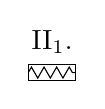
\begin{tikzpicture}[baseline=(word.base)]
\node[inner sep=1pt](word){$\mathrm{II}_1$.};
\draw[line width=.45pt]([yshift=-1mm]word.south west)rectangle([yshift=-3mm]word.south east);
\draw[line width=.4pt,decorate,decoration={zigzag,segment length=1.6mm,amplitude=.7mm}]([yshift=-2mm]word.south west)--([yshift=-2mm]word.south east);
\end{tikzpicture}}

(по англ. и женщина).





\rotatebox{90}{\GelfandFitDiagram{\begin{tikzpicture}[baseline=(reference.base)]
\node[inner sep=1pt](reference){см. Наймарк.};
\draw[line width=.5pt]([yshift=-.4mm]reference.south west)--([yshift=-.4mm]reference.south east);
\draw[line width=.5pt]([yshift=-1.4mm]reference.south west)--([yshift=-1.4mm]reference.south east);
\draw[line width=.5pt]([yshift=-2.4mm]reference.south west)--([yshift=-2.4mm]reference.south east);
\end{tikzpicture}}}





Подкольцо кольца всех опер. в гильб. пр-ве наз. фактором, если

\begin{GelfandAdjacentEvidence}{GELFAND-P000289}{4}
1) [зачёркнуто: $\forall$?] $X\in M\Longrightarrow X^*\in M$.

\Unclear{GELFAND-P000289}{axiom-cancelled-sign}{После «1)» под косыми штрихами возможен квантор $\forall$; знак не восстановлен.}
\end{GelfandAdjacentEvidence}


2) $M$ слабо замкнут ($\forall$ посл. $X_n$ вход. слаб. предел).

3) Центр --- из опер., кратных $I$.

\begin{GelfandAdjacentEvidence}{GELFAND-P000289}{5}
\underline{Пример.} В кон.-мерном:





\SourceFigure{GELFAND-P000289}{block-matrix}{\par\smallskip\centering{\color{black}\GelfandFitDiagram{\begin{minipage}{68mm}\raggedright \GelfandFitDiagram{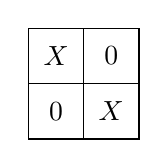
\begin{tikzpicture}[x=7mm,y=7mm]
\draw[line width=.6pt](0,0)rectangle(2,2);
\draw[line width=.6pt](1,0)--(1,2);
\draw[line width=.6pt](0,1)--(2,1);
\node at(.5,1.5){$X$};\node at(1.5,1.5){$0$};
\node at(.5,.5){$0$};\node at(1.5,.5){$X$};
\end{tikzpicture}}\end{minipage}}}\par\smallskip }
\end{GelfandAdjacentEvidence}


Всякий фактор в кон.-мерн. случае таков: в $H_1\otimes H_2$ надо рассм. опер. $X\otimes1$ ($X$ --- любой).

Вект. --- матрица $\xi_{ik}$. Опер. --- действ. на 1-ю координату.

\begin{center}\GelfandFitDiagram{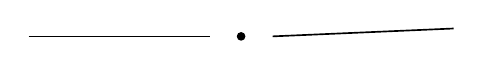
\begin{tikzpicture}[x=1mm,y=1mm]\draw[line width=.6pt](-27,0)--(-4,0);\fill(0,0)circle[radius=.55mm];\draw[line width=.6pt](4,0)--(27,1);\end{tikzpicture}}\end{center}

Всякое слабо замкнутое кольцо (с инволюцией) разлаг. в прям. интеграл факторов.

Фон Нейман \GelfandFitDiagram{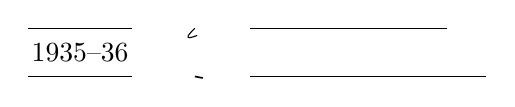
\begin{tikzpicture}[baseline=(years.base),x=1mm,y=1mm]
\node[inner sep=1pt](years)at(0,0){1935--36};
\draw[line width=.5pt]([yshift=1.5mm]years.north west)--([yshift=1.5mm]years.north east);
\draw[line width=.5pt]([yshift=-1.5mm]years.south west)--([yshift=-1.5mm]years.south east);
\draw[line width=.5pt]([xshift=15mm,yshift=1.5mm]years.north east)--([xshift=40mm,yshift=1.5mm]years.north east);
\draw[line width=.5pt]([xshift=15mm,yshift=-1.5mm]years.south east)--([xshift=45mm,yshift=-1.5mm]years.south east);
\draw[line width=.4pt]([xshift=8mm,yshift=1.5mm]years.north east)..controls([xshift=6.6mm,yshift=.2mm]years.north east)and([xshift=7mm,yshift=.1mm]years.north east)..([xshift=8.3mm,yshift=.6mm]years.north east);
\draw[line width=.6pt]([xshift=8mm,yshift=-1.5mm]years.south east)--([xshift=9mm,yshift=-1.7mm]years.south east);
\end{tikzpicture}}





Пусть $M$ --- фактор; тогда $\dfrac{X+X^*}{2}$, $\dfrac{X-X^*}{2i}$ их порождают.

(самосопр.) $a=\int\lambda\,de_\lambda$, $e_\lambda\in$ фактору, и порожд. фактор.

Фактор порожд. проекторами с $e^2=e$, $e^*=e$.



\Needspace{7\baselineskip}
\SourcePage{GELFAND-P000290}{56}
\hfill\GelfandFitDiagram{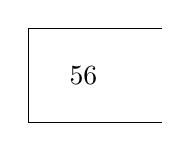
\begin{tikzpicture}[x=1mm,y=1mm]\draw(17,12)--(0,12)--(0,0)--(17,0);\node at(7,6){$56$};\end{tikzpicture}}

\begin{GelfandAdjacentEvidence}{GELFAND-P000290}{1}
Если [зачёркнуто: неразборчиво] сущ. \GelfandFitDiagram{\begin{tikzpicture}[baseline=(isometry.base)]
\node[inner sep=1pt](isometry){изометрия};
\node[draw,line width=.5pt,rounded corners=4pt,inner sep=1pt,anchor=south](partial)at([yshift=3mm]isometry.north){частичн.};
\draw[line width=.5pt](partial.south)--([yshift=.5mm]isometry.north);
\end{tikzpicture}} из $M$, соед. подпр-ва, соотв. проекторам, то 2 \GelfandFitDiagram{\begin{tikzpicture}[baseline=(operators.base)]
\node[inner sep=1pt](operators){опер.};
\node[anchor=north,inner sep=1pt]at([yshift=-.7mm]operators.south){(подпр.)};
\end{tikzpicture}} наз. эквивалентными.

\Unclear{GELFAND-P000290}{top-cancellation}{После «Если» перед «сущ.» высокие знаки густо перечёркнуты диагоналями; исходные знаки не разделены и не прочитаны.}
\end{GelfandAdjacentEvidence}










Если отожд. эквив., то \underline{получится упорядоченность} (по включ.).

Классы экв. проекц. опер. можно складывать.

Отсюда можно измерять подпр-ва (сопост. числа подпр-ву).

(Акс. Архим. нет --- $\infty$ есть).

\underline{\underline{Теор.}} Если есть $\min$ подпр., то оно изом. кольцу всех опер. в гильб. пр-ве.

\begin{equation*}R=M\otimes M'\qquad(M'\text{ --- коммут. фактор}).\end{equation*}

Нет $\min\Longrightarrow$ или $\mathrm{II}_1$, $\mathrm{II}_\infty$ или $\mathrm{III}$.

\begin{GelfandAdjacentEvidence}{GELFAND-P000290}{2}
$\mathrm{II}_1$ --- никогда нет $\min$, но всё измер. числами из $(0,1]$ (есть $\max$) и акс. Архим.









\SourceFigure{GELFAND-P000290}{type-II1-heading}{\par\smallskip\centering{\color{black}\GelfandFitDiagram{\begin{minipage}{68mm}\raggedright \GelfandFitDiagram{\begin{tikzpicture}[baseline=(heading.base),x=1mm,y=1mm]
\node[inner sep=1pt](heading)at(5,4){$\mathrm{II}_1$.};
\draw[line width=.6pt](0,0)--(11,.5);
\draw[line width=.6pt](0,-3)--(11,-2.5);
\draw[line width=.4pt](1,-2.9)--(1,-.1);
\draw[line width=.4pt](3,-2.8)--(3,.1);
\draw[line width=.4pt](5,-2.7)--(5,.2);
\draw[line width=.4pt](7.5,-2.6)..controls(6,-1.1)and(7,0)..(8,.3);
\draw[line width=.4pt](8.2,.3)..controls(8.2,-1.6)and(8.8,-1.5)..(9,-.3);
\end{tikzpicture}}\end{minipage}}}\par\smallskip }
\end{GelfandAdjacentEvidence}


\begin{GelfandAdjacentEvidence}{GELFAND-P000290}{3}
[зачёркнутый знак: $\forall$?] $\forall$ опер. имеет след и $\det$; Верна \underline{minimax} теория соб. знач. (всё, что для матриц).

\Unclear{GELFAND-P000290}{trace-cancelled-sign}{Перед читаемым $\forall$ малый знак с двумя наклонными штрихами и поперечиной зачёркнут. Возможное чтение $\forall$ не установлено.}
\end{GelfandAdjacentEvidence}


\begin{equation*}\operatorname{Tr}(a)=\int\lambda\,d(\dim e_\lambda)\qquad(\dim\text{ от }0\text{ до }1)\end{equation*}

Само пр-во ещё не открыто.

Какие факт. типа $\mathrm{II}_1$?

1) гиперфинитный Муррей и Нейман --- он один

2) Дж. Шварц

3) Ching

4) Sakai

5--6) Dixmier, Lance

7--8) Zeller-Meier

\begin{GelfandAdjacentEvidence}{GELFAND-P000290}{4}
$7,8'$) Степин, Голодец









\SourceFigure{GELFAND-P000290}{continuum-separator}{\par\smallskip\centering{\color{black}\GelfandFitDiagram{\begin{minipage}{68mm}\raggedright \GelfandFitDiagram{\begin{tikzpicture}[x=1mm,y=1mm]
\node[anchor=east,inner sep=1pt]at(-2,0){\shortstack{Континуум\\факторов}};
\draw[line width=.6pt](0,-6)--(1,6);
\draw[line width=.6pt](1.7,-6)--(2.7,6);
\node[anchor=west,inner sep=1pt]at(5,1){Dusa Mc Duff};
\end{tikzpicture}}\end{minipage}}}\par\smallskip }
\end{GelfandAdjacentEvidence}




\Needspace{7\baselineskip}
\SourcePage{GELFAND-P000291}{unlabelled}
\underline{$13/\mathrm{X}$-69 г.}\hfill\underline{След. раз Минлос и Синай.}

\underline{Гельфанд.}

\GelfandFitDiagram{\begin{tikzpicture}[baseline=(work.base)]
\node[inner sep=1pt](work){О раб. Араки.};
\draw[line width=.55pt,decorate,decoration={snake,amplitude=.5mm,segment length=2.5mm}]([yshift=-1mm]work.south west)--([yshift=-1mm]work.south east);
\end{tikzpicture}}





\underline{\underline{Вопрос:}} Пусть

\begin{equation*}
\begin{pmatrix}\alpha(t)&\beta(t)\\-\bar\beta(t)&\overline{\alpha(t)}\end{pmatrix}=u(t)
\end{equation*}

унит. матр. с $\det1$,

\begin{equation*}|\alpha(t)|^2+|\beta(t)|^2=1,\qquad t\in[0,1].\end{equation*}

Найти все неприв. унит. представления этой группы. Это не сделано.

$\operatorname{supp}$ предст. $F$ --- наим. замкн. мн-во, для к-рого вып. усл.

\begin{equation*}u(t)\equiv1\quad\forall t\in U(F)\Longrightarrow T_{u(t)}=I\end{equation*}

\underline{Задача:} сущ. ли неприв. унит. представл. с $\operatorname{supp}$ --- отрезок.

\begin{center}\GelfandFitDiagram{\begin{tikzpicture}[x=1mm,y=1mm]\draw[line width=.55pt](-18,0)--(-4,0);\fill(0,0)circle[radius=.35mm];\draw[line width=.55pt](4,0)--(18,0);\end{tikzpicture}}\end{center}

$\operatorname{supp}$ --- точка --- оператор $u(t_0)$ (2-мерн. предст.).

Это предст. $\delta(t-t_0)$.

\begin{GelfandAdjacentEvidence}{GELFAND-P000291}{1}
\begin{equation*}e:\ u(t)\longrightarrow T^e_{u(t_0)}\qquad\delta_e(t-t_0)\end{equation*}

\Unclear{GELFAND-P000291}{representation-index}{Перед двоеточием, над $T$ и под $\delta$ петлеобразный знак: $e$ / $\ell$. В набранной строке показан визуальный кандидат $e$; выбор буквы не установлен.}
\end{GelfandAdjacentEvidence}


\begin{equation*}u(t)\longrightarrow u(t_1)\otimes u(t_2)\end{equation*}

неприв. предст. с $\operatorname{supp}$ --- пара точек.

\begin{GelfandAdjacentEvidence}{GELFAND-P000291}{2}
(предст. по сути дела прям. суммы 2-х [зачёркнуто: матр.?] групп матр.).

\Unclear{GELFAND-P000291}{right-cancelled-word}{Скобочная приписка находится справа. После «2-х» зачёркнуто короткое слово, возможное чтение «матр.»; ниже отдельно «групп матр.». Чтение отменённого слова не установлено.}
\end{GelfandAdjacentEvidence}


Можно $n$ точек.

Для счётн. мн-ва нельзя уже сделать (можно для сход. послед.).

\GelfandFitDiagram{\begin{tikzpicture}[baseline=(araki.base)]
\node[inner sep=1pt](araki){Араки.};
\draw[line width=.55pt]([yshift=-.8mm]araki.south west)rectangle([yshift=-2.8mm]araki.south east);
\draw[line width=.45pt,decorate,decoration={zigzag,segment length=1.8mm,amplitude=.7mm}]([yshift=-1.8mm]araki.south west)--([yshift=-1.8mm]araki.south east);
\end{tikzpicture}}





Идея:

\begin{equation*}e^K=\bigoplus_{n=0}^{\infty}S^n(K)\end{equation*}

($K$ --- гильб. пр-во)

\begin{GelfandAdjacentEvidence}{GELFAND-P000291}{3}
\begin{equation*}e^{\varphi}=\bigoplus_{n=0}^{\infty}\frac{1}{\sqrt{n!}}\varphi\otimes\varphi\otimes\cdots\otimes p\end{equation*}

\Unclear{GELFAND-P000291}{coherent-last-symbol}{Последний множитель после $\otimes$ имеет нисходящий штрих и верхнюю правую петлю: $p$ / $\rho$; возможное отождествление с предыдущими $\varphi$ не установлено. В формуле показан визуальный кандидат $p$.}
\end{GelfandAdjacentEvidence}


$\sqrt{n!}$, чтобы $(e^{\varphi},e^{\psi})=e^{(\varphi,\psi)}$.

$K\to e^K$ --- функториальный переход

\begin{equation*}K_1\oplus K_2\longrightarrow e^{K_1}\otimes e^{K_2}\end{equation*}

В $\forall$ точке $t$ задаём представление в пр-ве $K(t)$ (напр. 2-мерном)

\begin{equation*}\int_0^1 K(t)\,dt\end{equation*}



\Needspace{7\baselineskip}
\SourcePage{GELFAND-P000292}{57}
\hfill\GelfandFitDiagram{\begin{tikzpicture}[x=1mm,y=1mm]\draw(0,13)--(0,0)--(17,1);\node at(7,6){$57$};\end{tikzpicture}}

Рассм. $e^{\int_0^1 K(t)\,dt}$.

Получается в нём (из функт.) предст., к-рое приводимо.

\begin{center}\GelfandFitDiagram{\begin{tikzpicture}[x=1mm,y=1mm]\draw[line width=.55pt](-20,0)--(-3,0);\fill(0,0)circle[radius=.4mm];\draw[line width=.55pt](3,0)--(20,.4);\end{tikzpicture}}\end{center}

Гр. матр. 1-го порядка $\alpha(t)=e^{x(t)}$.

\begin{GelfandAdjacentEvidence}{GELFAND-P000292}{1}
Непр. предст.

\Unclear{GELFAND-P000292}{representation-abbreviation}{В источнике сокращение «Непр.» перед «предст.»; раскрытие сокращения не установлено.}
\end{GelfandAdjacentEvidence}


\begin{gather*}e^{x(t)}\longrightarrow C,\qquad e^{x_1(t)}e^{x_2(t)}\longrightarrow C_1C_2,\qquad C=e^a\\x(t)\longrightarrow a\end{gather*}

\begin{GelfandAdjacentEvidence}{GELFAND-P000292}{2}
$a$ --- лин. ф-л от $X(t)$ --- обобщ. ф-я или распред.

\Unclear{GELFAND-P000292}{argument-case}{В строке о линейном функционале буква $X(t)$ / $x(t)$ крупнее соседних $x$; регистр не установлен. Показан кандидат $X(t)$.}
\end{GelfandAdjacentEvidence}


\begin{equation*}\delta(t-t_0):\qquad e^{x(t)}\longrightarrow e^{x(t_0)}\end{equation*}

\begin{equation*}x(t)\longrightarrow e^{\int_0^1 a(t)x(t)\,dt}\end{equation*}

На окружности добав. усл. целочисленности.

\begin{center}\GelfandFitDiagram{\begin{tikzpicture}[x=1mm,y=1mm]\draw[line width=.55pt](-11,0)--(-3,0);\fill(0,0)circle[radius=.4mm];\draw[line width=.55pt](3,0)--(11,.4);\end{tikzpicture}}\end{center}

Предст. здесь --- обобщение распределения.



\Needspace{7\baselineskip}
\SourcePage{GELFAND-P000293}{60}
\hfill\GelfandFitDiagram{\begin{tikzpicture}[x=1mm,y=1mm]\draw(0,13)--(0,0)--(17,1);\node at(7,6){$60$};\end{tikzpicture}}

\uwave{17/XI-69 г.}\qquad\underline{Хьюитт.}

\uwave{Один результат} (точный для всех \underline{комп.} групп)

как для окружности.





\begin{GelfandAdjacentEvidence}{GELFAND-P000293}{1}
[зачёркнуто: неразборчиво]

\Unclear{GELFAND-P000293}{upper-cancelled-sign}{Перед заголовком «Про s-числа» плотные пересекающиеся штрихи; исходные буквы или знаки не прочитаны.}
\end{GelfandAdjacentEvidence}


\begin{GelfandAdjacentEvidence}{GELFAND-P000293}{970}
\underline{Про $s$-числа:}

\begin{flushright}\begin{minipage}{.76\linewidth}
\underline{Гантмахер;}\par
\underline{Wielandt}\par
\underline{Березин, Гельфанд}\qquad Труды \underline{М.М.О.} ---\par
--- \underline{$\forall$ полупр. группы Ли.}\par
из теор. предст. для компл. ф-и.
\end{minipage}\end{flushright}\end{GelfandAdjacentEvidence}





\underline{H. Weyl}\qquad\underline{и}\qquad\underline{Ky Fan.}

\begin{GelfandAdjacentEvidence}{GELFAND-P000293}{2}
[зачёркнуто: неразборчиво] Всё это для произв. группы и класса представлений:

\Unclear{GELFAND-P000293}{middle-cancelled-sign}{Перед «Всё это» слитные вертикальные и косые штрихи зачёркнуты; исходная последовательность не установлена.}
\end{GelfandAdjacentEvidence}


\begin{GelfandAdjacentEvidence}{GELFAND-P000293}{3}
\begin{equation*}\|\hat f\|_p=(\sum_{\sigma\in\Sigma}d_\sigma\|\hat f(\sigma\|_p^p)\end{equation*}

\Unclear{GELFAND-P000293}{p-norm-formula}{После $\sigma$ в аргументе две вертикальные черты без отдельной закрывающей круглой скобки. За большой правой скобкой показатель не прочитан. При $d$ знак $\sigma$ допускает индексное либо строчное положение; показан кандидат $d_\sigma$.}
\end{GelfandAdjacentEvidence}


\underline{Теор. Петера-Вейля --- Планшереля}

\begin{equation*}\|\hat f\|_2^2=\int_G|f|^2\,d\lambda;\end{equation*}

\begin{GelfandAdjacentEvidence}{GELFAND-P000293}{4}
\begin{equation*}\|\hat f\|_\infty=\sup\{\|\hat f(\sigma)\|_{\mathfrak{S}_\infty}:\ \sigma\in\Sigma\}.\end{equation*}

\Unclear{GELFAND-P000293}{infinity-norm-subscript}{Перед $\infty$ S-образный знак с длинным пересекающим штрихом: $\mathfrak{S}_\infty$ / $S_\infty$. В этой строке показан готический кандидат; в следующей лемме сохранён обычный $S$.}
\end{GelfandAdjacentEvidence}


\underline{Лемма Рим.-Лебега:}

\begin{equation*}\forall f\in L_1(G),\quad\forall\varepsilon>0\quad\{\sigma:\ \|\hat f(\sigma)\|_{S_\infty}>\varepsilon\}\end{equation*}

--- конечное мн-во.

\underline{\underline{Т. Кунца.}}\qquad$1<p<2$

\begin{equation*}\|\hat f\|_{p\prime}\le\|f\|_p.\end{equation*}

\begin{GelfandAdjacentEvidence}{GELFAND-P000293}{5}
(Хаусд.-Юн.).

\Unclear{GELFAND-P000293}{young-abbreviation}{После «Хаусд.-» сокращение Юн. / Юнг.; конечный загнутый штрих перед точкой не установлен как часть н либо отдельная г.}
\end{GelfandAdjacentEvidence}


\underline{Теор.} Харди-Литтлевуда --- рав. лишь для \GelfandFitDiagram{\begin{tikzpicture}[baseline=(equality.base)]
\node[inner sep=1pt](equality){$f(x)=\alpha e^{inx};$};
\draw[line width=.55pt]([yshift=1mm]equality.south west)--([yshift=-1mm]equality.south west)--([yshift=-1mm]equality.south east)--([yshift=1mm]equality.south east);
\end{tikzpicture}}





Для общ. группы всё не так просто: там для ф-й вида

$\chi$ --- непр. ф-я на откр. подгруппе $G_0$,\quad$\chi(e)=1$,\quad$\chi(xy)=\chi(x)\chi(y)$,

$\chi=0$ вне $G_0$.

Аналоги теорем Рисса-Торина есть.



\Needspace{7\baselineskip}
\SourcePage{GELFAND-P000294}{unlabelled}
\GelfandFitDiagram{\begin{tikzpicture}[baseline=(date.base)]
\node[inner sep=1pt](date){23.2.70 г.};
\draw[line width=.6pt]([yshift=-.8mm]date.south west)rectangle([yshift=-2.5mm]date.south east);
\draw[line width=.5pt,decorate,decoration={zigzag,segment length=2mm,amplitude=.6mm}]([yshift=-1.65mm]date.south west)--([yshift=-1.65mm]date.south east);
\end{tikzpicture}}





\begin{GelfandAdjacentEvidence}{GELFAND-P000294}{1}
\underline{\underline{Каждан}} \underline{\underline{о}} \underline{\underline{раб.}} \underline{\underline{Гриффитса.}}





\Unclear{GELFAND-P000294}{upper-left-sketch}{Слева овальный контур с точкой внутри и шестью длинными кривыми сверху. У левого края маленькая петля и почти параллельные нижние штрихи. Связность коротких штрихов и продолжения кривых не установлены; подписей и уверенных стрелок нет.\par\smallskip\centering{\color{black}\GelfandFitDiagram{\begin{minipage}{68mm}\raggedright \GelfandFitDiagram{\begin{tikzpicture}[x=.2mm,y=.2mm]
\draw[line width=.55pt](28,60)..controls(0,34)and(17,6)..(64,5)..controls(99,-1)and(158,20)..(152,58)..controls(153,87)and(115,92)..(85,88)..controls(61,89)and(39,76)..(28,60);
\fill(83,50)circle[radius=2.4];
\draw[line width=.5pt](21,203)..controls(9,167)and(0,80)..(22,52);
\draw[line width=.5pt](47,198)..controls(35,169)and(22,84)..(30,61)..controls(34,54)and(36,51)..(45,52);
\draw[line width=.5pt](73,198)..controls(58,171)and(48,59)..(68,18);
\draw[line width=.5pt](85,174)..controls(87,145)and(81,90)..(87,85)..controls(89,72)and(95,65)..(101,63);
\draw[line width=.5pt](110,172)..controls(104,144)and(98,68)..(106,48)..controls(111,43)and(115,38)..(121,37);
\draw[line width=.5pt](129,161)..controls(130,135)and(126,65)..(128,42);
\draw[line width=.5pt](40,57)..controls(42,45)and(49,25)..(55,16);
\draw[line width=.45pt](21,58)..controls(17,50)and(28,44)..(36,53);
\end{tikzpicture}}\end{minipage}}}\par\smallskip }
\end{GelfandAdjacentEvidence}


\begin{equation*}T:\ H^i(V_s)\longrightarrow H^i(V_s)\end{equation*}

(при обходе вокруг вык. точки)

\begin{equation*}\exists N,\ \text{что}\quad(T^N-1)^{i+1}=0\end{equation*}

\begin{GelfandAdjacentEvidence}{GELFAND-P000294}{2}
($T$ унипотентно).

\Unclear{GELFAND-P000294}{monodromy-qualification}{После формулы отдельно написано «($T$ унипотентно)», без $N$ у $T$ и без приставки «квази»; запись сохранена.}
\end{GelfandAdjacentEvidence}


\begin{GelfandAdjacentEvidence}{GELFAND-P000294}{3}
\begin{center}\GelfandFitDiagram{\begin{tikzpicture}[x=1mm,y=1mm]\draw[line width=.55pt](-30,0)--(-4,0);\fill(0,0)circle[radius=.35mm];\draw[line width=.55pt](4,0)--(30,0);\end{tikzpicture}}\end{center}





\SourceFigure{GELFAND-P000294}{bundle-W}{\par\smallskip\centering{\color{black}\GelfandFitDiagram{\begin{minipage}{68mm}\raggedright \GelfandFitDiagram{\begin{tikzpicture}[x=1mm,y=1mm]\node at(0,15){$W$};\draw[->,line width=.65pt](0,11)--(0,3);\node at(0,0){$S$};\end{tikzpicture}}\end{minipage}}}\par\smallskip }
\end{GelfandAdjacentEvidence}


алгебраич. расслоение

база --- 1-мерн. алг. мн-зие (рим. пов. с выкол. точками).

\begin{equation*}\pi_1(S):\ H^K(V_s)\longrightarrow H^K(V_s)\qquad(\text{коэфф. }C).\end{equation*}

\begin{GelfandAdjacentEvidence}{GELFAND-P000294}{4}
\uwave{и опред. вект. расслоение} [зачёркнуто: неразборчивый знак] (аналитическое)

\Unclear{GELFAND-P000294}{cancelled-bundle-sign}{Между «расслоение» и «(аналитическое)» узкий перечёркнутый знак; первоначальная буква не установлена.}
\end{GelfandAdjacentEvidence}
\begin{GelfandAdjacentEvidence}{GELFAND-P000294}{5}






\SourceFigure{GELFAND-P000294}{bundle-E}{\par\smallskip\centering{\color{black}\GelfandFitDiagram{\begin{minipage}{68mm}\raggedright \GelfandFitDiagram{\begin{tikzpicture}[x=1mm,y=1mm]\node at(0,15){$E$};\draw[->,line width=.65pt](0,11)--(0,3);\node at(0,0){$S$};\end{tikzpicture}}\end{minipage}}}\par\smallskip }
\end{GelfandAdjacentEvidence}


$O(E)$ --- пучок ростков аналит. сеч.

Есть канонич. связность из паралл. переносов на универс. накрывающей $\tilde S$. (Там прям. произв.)

Будем изуч. вблизи выколотой точки.

Запишем связность в виде ур-я.

\begin{equation*}\begin{array}{l}f_1(z)\text{ --- сечения}\\\ldots\\f_n(z)\end{array}\qquad(\text{базис в окр. }z).\end{equation*}

\begin{GelfandAdjacentEvidence}{GELFAND-P000294}{6}
Ур. Пикара-Фукса $\dfrac{\partial}{\partial z}=A(z)$

\Unclear{GELFAND-P000294}{connection-operator}{В этой строке буквально $\partial/\partial z=A(z)$, без $f(z)$ по обе стороны. Ниже отдельно записано уравнение с $f(z)$; обе записи сохранены.}
\end{GelfandAdjacentEvidence}


\begin{GelfandAdjacentEvidence}{GELFAND-P000294}{7}
Перенесем $f_1(z)$ горизонт. в $z+\delta z$ и разложим по базису [зачёркнуто: $z+\delta z$, далее неразборчиво] $f_1(z+\delta z),\ldots$

\Unclear{GELFAND-P000294}{cancelled-basis-formula}{После «базису» отменённая последовательность $z+\delta z$ с неразборчивым концом; возможно, справа ещё $z$. Незачёркнутое $f_1(z+\delta z),\ldots$ прочитано отдельно.}
\end{GelfandAdjacentEvidence}


Рассм. любое плоское сеч. расслоения. оно удовл. ур-ю

\begin{equation*}\frac{\partial}{\partial z}f(z)=A(z)f(z)\end{equation*}

и все плоск. сеч. --- решения этого ур-я.

\begin{GelfandAdjacentEvidence}{GELFAND-P000294}{940}
\underline{\underline{Пример плоских сечений.}}

Пусть $\Phi_z$ --- цикл в слое ($K$-мерный).

\Unclear{GELFAND-P000294}{overwritten-cycle}{После «Пусть» крупная густо обведённая буква: $\Phi_z$ / $\phi_z$; исходный вид и повторное обведение либо исправление не установлены. Показан кандидат $\Phi_z$.}
\end{GelfandAdjacentEvidence}


\begin{equation*}\Phi_z\subset V_z,\qquad\Phi_{z'}\subset V_{z'}.\end{equation*}



\Needspace{7\baselineskip}
\SourcePage{GELFAND-P000295}{62}
\hfill\GelfandFitDiagram{\begin{tikzpicture}[x=1mm,y=1mm]\draw(0,13)--(0,0)--(17,1);\node at(7,6){$62$};\end{tikzpicture}}





\begin{GelfandAdjacentEvidence}{GELFAND-P000295}{1}
--- пример плоского сечения. ---

\Unclear{GELFAND-P000295}{pairing-index}{Первая запись имеет две пары круглых скобок; внешние вытянуты вниз к пояснению. После $f$ обведённый знак: $f_i(z)$ / $f^i(z)$. Показан нижний $i$; отношение скобок к нижнему пояснению не установлено.\par\smallskip\centering{\color{black}\GelfandFitDiagram{\begin{minipage}{68mm}\raggedright \GelfandFitDiagram{\begin{tikzpicture}[x=1mm,y=1mm]
\node[inner sep=1pt]at(0,6){$(f_i(z),\phi_z)$};
\node[inner sep=1pt]at(2,-3){знач. когом. на гом.};
\draw[line width=.55pt](-23,14)..controls(-28,9)and(-28,-5)..(-22,-7);
\draw[line width=.55pt](23,14)..controls(26,8)and(26,-2)..(23,-4);
\end{tikzpicture}}\end{minipage}}}\par\smallskip }
\end{GelfandAdjacentEvidence}


\hfill --- вектор-ф-я.





\underline{\underline{Теор.}} (Гриффитс)

$\exists$ такой базис $f_i(z)$, чтобы ур-е имело рег. особую точку,

т.е. $zA(z)$ голоморфно продолжается в $0$. (регулярно).

(Позв. судить о повед. периодов при прибл. к особой точке).

\begin{GelfandAdjacentEvidence}{GELFAND-P000295}{950}
\underline{Следствие}

Рассм. любое плоск. сечение --- реш. ур-я. Тогда оно разлаг. в ряд

\begin{equation*}\sum_{n\le0}z^{n/N}\big(\underline{C_{n0}}+\underline{C_{n1}}\ln z+\ldots+\underline{c_{nk}}\ln^k z\big)\end{equation*}

\Unclear{GELFAND-P000295}{series-indices}{Индекс $n$ / $\nu$ густо обведён. Знак границы похож на $\le$; показано $n\le0$, верхний предел не установлен. Последняя первая буква меньше первых $C$, c-/e-подобная; регистр и чтение не установлены, показан кандидат $c_{nk}$. Три коэффициента подчёркнуты.}
\end{GelfandAdjacentEvidence}


\begin{GelfandAdjacentEvidence}{GELFAND-P000295}{940}
\underline{\underline{Лемма}}\qquad$\forall$ плоск. сеч. $\phi_z$

\begin{equation*}|\Phi_z|\le C|z|^{-a}|\ln z|^b\end{equation*}

\Unclear{GELFAND-P000295}{bound-exponent}{Показатель у $|\ln z|$ имеет две тесные петли: $b$ / $\beta$. Показан $b$. В самой оценке крупное $\Phi$, а в предыдущей строке более лёгкое $\phi$; различие сохранено.}
\end{GelfandAdjacentEvidence}
\begin{GelfandAdjacentEvidence}{GELFAND-P000295}{4}






\SourceFigure{GELFAND-P000295}{lower-dotted-rule}{\par\smallskip\centering{\color{black}\GelfandFitDiagram{\begin{minipage}{68mm}\raggedright $\cdot\quad\cdot\quad\cdot\quad\cdot\quad\cdot\quad\cdot\quad\cdot\quad\cdot\quad\cdot\quad\cdot\quad\cdot\quad\cdot$\end{minipage}}}\par\smallskip }
\end{GelfandAdjacentEvidence}




\Needspace{7\baselineskip}
\SourcePage{GELFAND-P000296}{unlabelled}
7/IX-1970 г.\qquad\GelfandFitDiagram{\begin{tikzpicture}[baseline=(word.base)]
\node[inner sep=1pt](word){Семинар};
\draw[line width=.55pt]([yshift=-.8mm]word.south west)rectangle([yshift=-2.5mm]word.south east);
\draw[line width=.45pt,decorate,decoration={zigzag,segment length=2mm,amplitude=.6mm}]([yshift=-1.65mm]word.south west)--([yshift=-1.65mm]word.south east);
\end{tikzpicture}} \GelfandFitDiagram{\begin{tikzpicture}[baseline=(word.base)]
\node[inner sep=1pt](word){Гельфанда.};
\draw[line width=.55pt]([yshift=-.8mm]word.south west)rectangle([yshift=-2.5mm]word.south east);
\draw[line width=.45pt,decorate,decoration={zigzag,segment length=2mm,amplitude=.6mm}]([yshift=-1.65mm]word.south west)--([yshift=-1.65mm]word.south east);
\end{tikzpicture}}





\underline{Программа семинара.}

1. Каждан о связи формальной и алгебраич. геометрии.

2. Арнольд: Работы Гриффитса.

3. Митягин и Хенкин об их работах.

\begin{GelfandAdjacentEvidence}{GELFAND-P000296}{1}
[зачёркнутый номер: 4.?] $1^{\prime}$. Мойшезон о работах Артина.

\Unclear{GELFAND-P000296}{cancelled-programme-number}{Перед отдельным незачёркнутым $1^{\prime}$ густо отменён номер или знак, возможное чтение 4.; номер не восстановлен.}
\end{GelfandAdjacentEvidence}


?. $K$-теория конечных групп

\hfill Браун, Тейт, Томсон, Суон, Кац.

(Каждан, Бернштейн и т.д.)

4. Хиронака.

\begin{GelfandAdjacentEvidence}{GELFAND-P000296}{950}
\underline{На след. семестр.}

$\zeta$-ф-я\qquad($p$-адич. гарм. анализ).

Конечные группы.\end{GelfandAdjacentEvidence}

\begin{center}\GelfandFitDiagram{\begin{tikzpicture}[x=1mm,y=1mm]\draw[line width=.55pt](-30,0)--(-4,0);\fill(0,0)circle[radius=.5mm];\draw[line width=.55pt](4,0)--(30,0);\end{tikzpicture}}\end{center}

\underline{\underline{Каждан.}}

Где это изложено?





\begin{GelfandAdjacentEvidence}{GELFAND-P000296}{2}
ч. \underline{III}, $N=1$.

\SourceFigure{GELFAND-P000296}{cohomology-bracket}{\par\smallskip\centering{\color{black}\GelfandFitDiagram{\begin{minipage}{68mm}\raggedright \GelfandFitDiagram{\begin{tikzpicture}
\node[inner sep=2pt](refs){\begin{minipage}{.78\linewidth}1. Серр «Когер. алг. пучки».\par\smallskip
2. Более совр., но менее приятное\qquad Дьёдонне\qquad Мат. 9:1\par\smallskip
3. Лекции Ю.И. Манина (часть 1)\qquad Алг. геометрия.\par\smallskip
4. 3-й том Гротендика\qquad I.H.E.S., т.12\end{minipage}};
\draw[line width=.55pt]([xshift=1mm,yshift=-1mm]refs.north west)--([xshift=-2mm,yshift=-1mm]refs.north west)--([xshift=-2mm,yshift=1mm]refs.south west)--([xshift=1mm,yshift=1mm]refs.south west);
\node[rotate=90,anchor=south,inner sep=1pt]at([xshift=-4mm]refs.west){\shortstack{Когомологии\\афф. и проект. схем.}};
\end{tikzpicture}}\end{minipage}}}\par\smallskip }
\end{GelfandAdjacentEvidence}


\underline{Замеч. Гельфанда:} выуч. кн. Серра «Кон. группы» и «Гр. Ли и алг. Ли».

\begin{GelfandAdjacentEvidence}{GELFAND-P000296}{3}
(Входят в минимум по лин. алгебре)





\SourceFigure{GELFAND-P000296}{parts-arrow}{\par\smallskip\centering{\color{black}\GelfandFitDiagram{\begin{minipage}{68mm}\raggedright \GelfandFitDiagram{\begin{tikzpicture}[x=1mm,y=1mm]
\draw[->,line width=.6pt](0,9)--(2,1);
\node[anchor=north west,inner sep=1pt]at(0,0){1 и 2-я часть.};
\end{tikzpicture}}\end{minipage}}}\par\smallskip }
\end{GelfandAdjacentEvidence}


\underline{1-я часть:}\qquad\GelfandFitDiagram{\begin{tikzpicture}[baseline=(part.base)]\node[inner sep=1pt](part){Когомологии когерентных пучков.};\draw[dashed,line width=.45pt]([yshift=-1mm]part.south west)--([yshift=-1mm]part.south east);\end{tikzpicture}}





\S1. \underline{Определение схемы.}

Схема --- окольцованное пр-во специального вида

\GelfandFitDiagram{\begin{tikzpicture}[baseline=(space.base)]
\node[inner sep=1pt](space){Топ. пр-во,};
\draw[line width=.5pt](space.south west)--([yshift=-1mm]space.south west)--([yshift=-1mm,xshift=5mm]space.south west)--([yshift=-5mm,xshift=5mm]space.south west)--([yshift=-5mm,xshift=-5mm]space.south east)--([yshift=-1mm,xshift=-5mm]space.south east)--([yshift=-1mm]space.south east);
\node[inner sep=1pt]at([yshift=-3mm]space.south){$X$};
\end{tikzpicture}} снабж. пучком колец. $O$\qquad(структ. пучок).





Аффинная схема.\qquad$A$ --- комм. кольцо с 1.

\begin{GelfandAdjacentEvidence}{GELFAND-P000296}{4}
$\operatorname{Spec}A$\qquad Точки --- простые идеалы $\wp\subset A$.

\Unclear{GELFAND-P000296}{prime-ideal-symbol}{Петлеобразный знак идеала: $\wp$ / $\mathfrak p$ / $p$. В обоих местах показано ближайшее доступное начертание $\wp$; тождество буквы не установлено.}
\end{GelfandAdjacentEvidence}


\begin{GelfandAdjacentEvidence}{GELFAND-P000296}{951}
Топология: $\forall$ \GelfandFitDiagram{\begin{tikzpicture}[baseline=(ideal.base)]\node[inner sep=1pt](ideal){$I$};\draw[line width=.45pt](ideal.south)--([yshift=-3mm]ideal.south);\node[anchor=north,inner sep=1pt]at([yshift=-3mm]ideal.south){идеалу};\end{tikzpicture}} $\subset A$ сопост. мн-во простых идеалов $U_I\subset\operatorname{Spec}A$,





сост. из прост. идеалов

\begin{equation*}\wp\quad\tikz[baseline=-.4ex,x=1em,y=1em]{\draw[line width=.55pt](0,.25)..controls(.95,.25)and(.95,-.25)..(0,-.25);\draw[line width=.55pt](.18,-.45)--(.50,.45);}\quad I.\end{equation*}

\Unclear{GELFAND-P000296}{crossed-inclusion}{Между знаком простого идеала и I округлый знак включения, открытый влево, перечёркнут косым штрихом. Отдельной нижней черты равенства не видно; она не добавлена. Точный смысл соглашения о включении не установлен.}
\end{GelfandAdjacentEvidence}


Мн-ва $U_I$ наз. открытыми.



\Needspace{7\baselineskip}
\SourcePage{GELFAND-P000297}{67}
\hfill\GelfandFitDiagram{\begin{tikzpicture}[x=1mm,y=1mm]\draw[line width=.55pt](0,13)--(0,0)--(17,1);\node at(7,6){$67$};\end{tikzpicture}}

\underline{Задача:} пров., что получ. топология.

Базис откр. множеств:

\begin{GelfandAdjacentEvidence}{GELFAND-P000297}{1}
\begin{equation*}f\in A\ \leadsto\ U_f\subset\operatorname{Spec}A\quad\text{из}\quad\wp\not\ni f.\end{equation*}

\Unclear{GELFAND-P000297}{prime-membership}{Петлеобразный знак идеала допускает $\wp$ / $\mathfrak p$ / $p$; показан кандидат $\wp$. Следующий знак имеет округлый контур, среднюю поперечину и пересекающий штрих; показано $\not\ni$.}
\end{GelfandAdjacentEvidence}


\underline{Задача:} $U_f$ --- базис.

\underline{Задача:} вып. самая слабая акс. отделимости
(из 2-х точек 1 можно отд. окр.)

\underline{Локализация.}

Пусть $S$ --- мультипл. мн-во в $A$, не содерж. $0$ (замкн. отн. умн.)

Кольцо $A_S$ сост. из пар $\dfrac a s$:

\begin{equation*}\frac a s=\frac{a^{\prime}}{s^{\prime}}\ \Longleftrightarrow\ \exists s^{\prime\prime}\in S\qquad s^{\prime\prime}(s^{\prime}a-sa^{\prime})=0.\end{equation*}

\underline{Задача:} это соотн. эквивал.

Позднее это понадобится для модулей.

Структ. пучок на $\operatorname{Spec}A$:

\begin{equation*}\Gamma(U_f,O)=A_{\substack{\{f^n\}\\n\ge0}},\qquad S=\{f^n\}.\end{equation*}

\begin{GelfandAdjacentEvidence}{GELFAND-P000297}{940}
\underline{Напоминание.}

\underline{Опр. пучка.}

Предпучок и $\forall U\subset X$ и покр. $\{U_\alpha^*\}$ мн-ва $U$ точна послед.

\begin{equation*}\{U_\alpha^*\}\subset U\qquad\left(\bigcup U_\alpha^*=U\right).\end{equation*}





\Unclear{GELFAND-P000297}{sheaf-product-sign}{В обоих местах окружности с плюсом, переданные как $\bigoplus$; под первым выражением «произвед. мн-в». Значение знаков не установлено.\par\smallskip\centering{\color{black}\GelfandFitDiagram{\begin{minipage}{148mm}\raggedright \GelfandFitDiagram{\begin{tikzpicture}[x=1mm,y=1mm]
\node[inner sep=1pt](first)at(0,0){$F(U)$};
\node[inner sep=1pt](second)at(44,0){$\underbrace{\displaystyle\bigoplus_\alpha F(U_\alpha)}_{\text{произвед. мн-в}}$};
\node[inner sep=1pt](third)at(113,0){$\displaystyle\bigoplus_{\alpha,\beta}F(U_\alpha\cap U_\beta).$};
\draw[->,line width=.6pt](first.east)--(second.west);
\draw[->,line width=.6pt]([yshift=1mm]second.east)--([yshift=1mm]third.west);
\draw[->,line width=.6pt]([yshift=-1mm]second.east)--([yshift=-1mm]third.west);
\end{tikzpicture}}\end{minipage}}}\par\smallskip }
\end{GelfandAdjacentEvidence}


\begin{equation*}F(U_\alpha)\longrightarrow F(U_\alpha\cap U_\beta)\end{equation*}

\begin{GelfandAdjacentEvidence}{GELFAND-P000297}{3}
\begin{equation*}F(U_\alpha)\longrightarrow F(U_\beta\cap U_\alpha)\end{equation*}

\Unclear{GELFAND-P000297}{restriction-corrections}{Во второй строке три индекса густо исправлены. Показано $F(U_\alpha)\to F(U_\beta\cap U_\alpha)$; левый индекс допускает $\alpha$ / $\beta$. Первоначальные штрихи не восстановлены.}
\end{GelfandAdjacentEvidence}


\underline{Вопрос:} почему это разные стрелки?

Точность:

\begin{equation*}\operatorname{Im}i=\{\,\cdot\mid\varphi_1=\varphi_2\}.\end{equation*}

Слой пучка (предп.) в т. $x$ и т.д.

\underline{Задача:} док., что $\forall$ предпучку $\exists$ пучок с теми же слоями
(и единств.)

\begin{GelfandAdjacentEvidence}{GELFAND-P000297}{4}
\underline{Замечание:} для опр. пучка предпучок дост. знать на базе.





\SourceFigure{GELFAND-P000297}{reminder-separator}{\par\smallskip\centering{\color{black}\GelfandFitDiagram{\begin{minipage}{68mm}\raggedright \GelfandFitDiagram{\begin{tikzpicture}[x=1mm,y=1mm]
\draw[line width=.5pt](-62,0)--(-48,0);\fill(-44,0)circle[radius=.35mm];\draw[line width=.5pt](-40,0)--(-16,0);
\node[anchor=west,inner sep=1pt]at(-4,0){\underline{Конец напоминания.}};
\end{tikzpicture}}\end{minipage}}}\par\smallskip }
\end{GelfandAdjacentEvidence}


\begin{GelfandAdjacentEvidence}{GELFAND-P000297}{5}
\begin{equation*}U_f\subset U_g\ \Longleftrightarrow\ \exists n:\quad f^m=gh.\end{equation*}

\Unclear{GELFAND-P000297}{inclusion-correction}{Знак между $U_f$ и $U_g$ густо исправлен; показан внешний контур $\subset$. Первоначальный знак не установлен.}
\end{GelfandAdjacentEvidence}
\begin{GelfandAdjacentEvidence}{GELFAND-P000297}{6}


\Unclear{GELFAND-P000297}{exponent}{После $\exists$ читается $n$; показатель у $f$ имеет несколько слитых дуг: $m$ / исправленное $n$. Показано $f^m$; совпадение с квантором не установлено.}
\end{GelfandAdjacentEvidence}


(Равнос. теор. о том, что $\bigcap$ всех пр. идеалов есть радикал)



\Needspace{7\baselineskip}
\SourcePage{GELFAND-P000298}{unlabelled}
\begin{equation*}A_{\{g^n\}}\longrightarrow A_{\{f^n\}}.\end{equation*}

\begin{equation*}\frac a g\longrightarrow\frac{ah}{f^m},\qquad\frac a{g^k}\longrightarrow\frac{ah^k}{f^{mk}}.\end{equation*}

\begin{GelfandAdjacentEvidence}{GELFAND-P000298}{1}
\begin{center}\GelfandFitDiagram{\begin{tikzpicture}[x=1mm,y=1mm]\draw[line width=.5pt](-30,0)--(-4,0);\fill(0,0)circle[radius=.35mm];\draw[line width=.5pt](4,0)--(30,0);\end{tikzpicture}}\end{center}





\SourceFigure{GELFAND-P000298}{definition-arrow}{\par\smallskip\centering{\color{black}\GelfandFitDiagram{\begin{minipage}{148mm}\raggedright \GelfandFitDiagram{\begin{tikzpicture}[x=1mm,y=1mm]
\node[anchor=north west,inner sep=1pt]at(0,0){\begin{minipage}{145mm}\underline{Предсхема:} окольцов. пр-во, лок. изом. афф. схеме.\par\medskip
\underline{Задача.} $\forall f\in A$, $(U_f,O)={}$ афф. схема\end{minipage}};
\draw[->,line width=.6pt](-7,2)..controls(-11,-5)and(-11,-13)..(-8,-19);
\end{tikzpicture}}\end{minipage}}}\par\smallskip }
\end{GelfandAdjacentEvidence}


\underline{Произведение предсхем.}\qquad$\operatorname{Spec}A,\ \operatorname{Spec}B$

\begin{equation*}\operatorname{Spec}A\times\operatorname{Spec}B=\operatorname{Spec}(A\otimes B)\end{equation*}

\begin{GelfandAdjacentEvidence}{GELFAND-P000298}{2}
\underline{\underline{Задача:}} определить опред. двух предсхем.

\Unclear{GELFAND-P000298}{task-word}{После «определить» короткое слово допускает «опред.» / «произв.»; показано «опред.». Повторение не устранено.}
\end{GelfandAdjacentEvidence}
\begin{GelfandAdjacentEvidence}{GELFAND-P000298}{3}






\SourceFigure{GELFAND-P000298}{framed-example}{\par\smallskip\centering{\color{black}\GelfandFitDiagram{\begin{minipage}{68mm}\raggedright \GelfandFitDiagram{\begin{tikzpicture}
\node[draw,line width=.6pt,rounded corners=9pt,inner sep=4pt](example){\begin{minipage}{65mm}\centering\underline{пример.}\par
$(Z_2$ и $Z_3)$.\par\smallskip
$\operatorname{Spec}Z_2\times\operatorname{Spec}Z_3$ ---\par
--- пустое мн-во.\end{minipage}};
\end{tikzpicture}}\end{minipage}}}\par\smallskip }
\end{GelfandAdjacentEvidence}


\begin{GelfandAdjacentEvidence}{GELFAND-P000298}{4}
\begin{center}\GelfandFitDiagram{\begin{tikzpicture}[x=1mm,y=1mm]\draw[line width=.55pt](-80,0)--(80,0);\end{tikzpicture}}\end{center}





\SourceFigure{GELFAND-P000298}{kirillov-frame}{\par\smallskip\centering{\color{black}\GelfandFitDiagram{\begin{minipage}{68mm}\raggedright \GelfandFitDiagram{\begin{tikzpicture}[baseline=(name.base)]
\node[inner sep=2pt](name){\shortstack{Импровиз.\\Кириллова}};
\draw[line width=.55pt](name.north west)--(name.north east)--(name.south east)--(name.south west);
\end{tikzpicture}}\end{minipage}}}\par\smallskip }
\end{GelfandAdjacentEvidence}


\begin{GelfandAdjacentEvidence}{GELFAND-P000298}{5}
\begin{equation*}\begin{array}{cc}X,&Y\\\Vert&\Vert\\\bigcup X_\alpha&\bigcup Y_\beta\end{array}\qquad\text{--- предсхемы}\end{equation*}

\Unclear{GELFAND-P000298}{gluing-y-corrections}{Буква $Y$ в покрытии и буквы $Y$ в правом пересечении густо обведены с дополнительными штрихами; конечные $Y$ читаются, первоначальные буквы не установлены.}
\end{GelfandAdjacentEvidence}


\begin{GelfandAdjacentEvidence}{GELFAND-P000298}{6}
в $\displaystyle\bigcup_\alpha(X_\alpha\times Y_\beta)$

\Unclear{GELFAND-P000298}{union-index}{Под знаком объединения маленький затушёванный индекс с петлёй и несколькими лучами: $\alpha$ / $*$ / исправленный знак. Показан кандидат $\alpha$; второй индекс не добавлен.}
\end{GelfandAdjacentEvidence}
\begin{GelfandAdjacentEvidence}{GELFAND-P000298}{7}






\SourceFigure{GELFAND-P000298}{gluing-layout}{\par\smallskip\centering{\color{black}\GelfandFitDiagram{\begin{minipage}{148mm}\raggedright \begin{equation*}\begin{array}{cc}
X_\alpha\times Y_\beta&X_{\alpha^{\prime}}\times Y_{\beta^{\prime}}\\[1em]
X_\alpha\cap X_{\alpha^{\prime}}&Y_\beta\cap Y_{\beta^{\prime}}\\
\Vert&\Vert\\
\bigcup X_\gamma&\bigcup Y_\delta
\end{array}\end{equation*}\end{minipage}}}\par\smallskip }
\end{GelfandAdjacentEvidence}


\underline{Лемма:} $X_\alpha\subset X_{\alpha^{\prime}}$, $Y_\beta\subset Y_{\beta^{\prime}}$ $\Rightarrow X_\alpha\times Y_\beta\subset X_{\alpha^{\prime}}\times Y_{\beta^{\prime}}$.

\underline{\underline{См. Серр.}}

\begin{center}\GelfandFitDiagram{\begin{tikzpicture}[x=1mm,y=1mm]\draw[line width=.55pt](-80,0)--(80,0);\end{tikzpicture}}\end{center}

\begin{GelfandAdjacentEvidence}{GELFAND-P000298}{8}
\underline{Предсхема $X$} наз. схемой, если $\Delta\subset X*X$ замкнута.

\Unclear{GELFAND-P000298}{diagonal-product}{Между $X$ и $X$ маленький многолучевой знак с тёмной серединой: $*$ / обведённое $\times$. Звёздочкообразная форма показана как $*$.}
\end{GelfandAdjacentEvidence}


\underline{Задача:} док., что афф. схема явл. схемой.

\begin{GelfandAdjacentEvidence}{GELFAND-P000298}{9}
Пусть $X$ --- произв. предсхема, $\mathcal F$ --- пучок $\mathcal O$-модулей
над [зачёркнут знак: $x$?] $X$.

\Unclear{GELFAND-P000298}{lower-correction}{Между «над» и $X$ густо зачёркнут одиночный знак, возможно $x$; исходная буква не установлена.}
\end{GelfandAdjacentEvidence}


\begin{GelfandAdjacentEvidence}{GELFAND-P000298}{940}
Он наз. квазикогерентным, если он лок. изом.



\Needspace{7\baselineskip}
\SourcePage{GELFAND-P000299}{68}
\hfill\GelfandFitDiagram{\begin{tikzpicture}[x=1mm,y=1mm]\draw[line width=.55pt](0,13)--(0,0)--(17,1);\node at(7,6){$68$};\end{tikzpicture}}

коядру отображения:

\begin{equation*}\underbrace{O^R}_{\text{прям. суммы.}}\overset{\varphi}{\longrightarrow}O^T.\end{equation*}

$S,T$ --- произвольные мн-ва.

\Unclear{GELFAND-P000299}{presentation-exponent}{Первый показатель густо обведён: $R$ / исправленное $S$. Показано $O^R\to O^T$; в следующей строке отдельно $S,T$. Под первым $O$ «прям. суммы.».}
\end{GelfandAdjacentEvidence}


\underline{Задача:} привести пример не квазикогер. пучка.

\underline{Теорема.} Пусть $A$ --- комм. кольцо и $\operatorname{Spec}A$ --- афф. сх.

Отобр. из катег. квазиког. пучков модулей

\begin{equation*}\mathcal F\longrightarrow\Gamma(\operatorname{Spec}A,\mathcal F)\end{equation*}

в катег. модулей есть изоморфизм.

Т. е. катег. к.-к. пучков мод. над афф. сх. $A$ изом.
катег. модулей над $A$.

(Модуль глоб. сечений.)

\begin{GelfandAdjacentEvidence}{GELFAND-P000299}{2}
(Это равносильно тому, что для афф. пр-в когом. нулевые)

\Unclear{GELFAND-P000299}{cohomology-qualification}{В этой отдельной фразе степени когомологий и коэффициенты не указаны.}
\end{GelfandAdjacentEvidence}


Квазикогер. пучок модулей опред. своими глоб. сечениями.

$28/\overline{\underline{\mathrm{IX}}}$.

\underline{Прямой и обр. образ пучков.}

\begin{equation*}X\overset f{\longrightarrow}Y,\qquad X,Y\text{ --- топ. пр-ва,}\end{equation*}

$\mathcal F$ --- пучок на $X$,

\begin{equation*}\Gamma(U,f_*\mathcal F):=\Gamma(f^{-1}(U),\mathcal F),\qquad U\subset Y\end{equation*}

получается предпучок на $Y$.

\underline{Упражнение} (лёгкое) --- этот предпучок явл. пучком

\begin{GelfandAdjacentEvidence}{GELFAND-P000299}{940}
\underline{Пример:} если $Y$ --- точка, то $f_*\mathcal F$ --- группа сечений исх. пучка,

($f^{-1}(U)$ может быть и пусто, тогда мн-во сечений пусто).

\Unclear{GELFAND-P000299}{empty-sections}{В источнике дважды «пусто»: «может быть и пусто, тогда мн-во сечений пусто»; оба слова переданы буквально.}
\end{GelfandAdjacentEvidence}


\uwave{Очень важное понятие.}

\underline{Обратный образ.}

\begin{equation*}X\overset f{\longrightarrow}Y\end{equation*}

$\mathcal G$ --- пучок на $Y$



\Needspace{7\baselineskip}
\begin{GelfandAdjacentEvidence}{GELFAND-P000300}{950}
\SourcePage{GELFAND-P000300}{unlabelled}
Пучок $f^*\mathcal G$ определяется так:

$\forall\mathcal F$ на $X$ справедливо равенство:





\Unclear{GELFAND-P000300}{Hom-callout}{Над правым краем рамки номер с закрывающей скобкой густо обведён: 1) / исправленный номер. Показан кандидат 1). Под левым Hom вертикальный штрих ведёт к подписи «мн-во морфизмов над X».\par\smallskip\centering{\color{black}\GelfandFitDiagram{\begin{minipage}{148mm}\raggedright \GelfandFitDiagram{\begin{tikzpicture}
\node[draw,line width=.6pt,inner sep=4pt](hom){$\operatorname{Hom}(f^*\mathcal G,\mathcal F)=\operatorname{Hom}(\mathcal G,f_*\mathcal F)$};
\node[anchor=south west,inner sep=1pt]at(hom.north east){$^{1)}$};
\draw[line width=.5pt]([xshift=18mm]hom.south west)--([xshift=18mm,yshift=-5mm]hom.south west);
\node[anchor=north,inner sep=1pt]at([xshift=24mm,yshift=-5mm]hom.south west){\shortstack{мн-во морфизмов\\над $X$}};
\end{tikzpicture}}\end{minipage}}}\par\smallskip }
\end{GelfandAdjacentEvidence}


Т. е. $\forall$ пучка $\mathcal F$ задано вз.-однозн. отобр. этих мн-в,
согласованные при морфизмах $\mathcal F$ друг в друга.

(Изоморфизм функторов на кат. пучков).

\uwave{Конструкция}, доказ. существование $f^*\mathcal G$

\begin{GelfandAdjacentEvidence}{GELFAND-P000300}{2}
[Зачёркнуто короткое выражение: ?]

\Unclear{GELFAND-P000300}{cancelled-formula}{Под несколькими диагоналями видны Γ/F-подобная буква, круглые контуры и U-подобный знак: $F(U)$ / $\Gamma(U,\mathcal G)$; состав не установлен.}
\end{GelfandAdjacentEvidence}


\begin{GelfandAdjacentEvidence}{GELFAND-P000300}{3}
\begin{equation*}\Gamma(U,\overline{f^*\mathcal G})=\underset{\substack{\longrightarrow\\V\supset f(U)}}{\lim}\Gamma(V,\mathcal G)\end{equation*}

\Unclear{GELFAND-P000300}{limit-variable}{Первый аргумент последнего $\Gamma$ густо исправлен: $V$ / $U$ / повторно обведённое $V$. Показано $V$; первоначальные штрихи не установлены.}
\end{GelfandAdjacentEvidence}


это рав-во опред. предпучок\qquad $(V\subset Y)$

\begin{GelfandAdjacentEvidence}{GELFAND-P000300}{4}
\underline{Упражн.:} ассоц. с ним пучок есть обратный образ





\SourceFigure{GELFAND-P000300}{two-point-example}{\par\smallskip\centering{\color{black}\GelfandFitDiagram{\begin{minipage}{148mm}\raggedright \GelfandFitDiagram{\begin{tikzpicture}[x=1mm,y=1mm]
\node[anchor=north west,inner sep=1pt](example)at(0,0){\begin{minipage}{142mm}\underline{Пример.}\par\smallskip
\begin{tikzpicture}[x=1mm,y=1mm]
\node at(-10,0){$X=$};\fill(0,0)circle[radius=.65mm];\fill(13,0)circle[radius=.65mm];
\draw[line width=.5pt](0,5)--(0,11);\node[anchor=east,inner sep=1pt]at(-1,9){$\mathcal G$};
\draw[line width=.5pt](13,5)--(13,11);\node[anchor=west,inner sep=1pt]at(14,9){$\mathcal G$};
\node at(55,0){$Y=$};\fill(65,0)circle[radius=.65mm];\draw[line width=.5pt](65,6)--(65,17);\node[anchor=west,inner sep=1pt]at(66,14){$\mathcal G$};
\end{tikzpicture}\par\smallskip
Когда $U\subset X$ есть точка, то $\mathcal G$, $U=X$ --- тоже $\mathcal G$. \underline{Не пучок.}\end{minipage}};
\draw[line width=.9pt]([xshift=-2mm]example.north west)..controls([xshift=-6mm]example.north west)and([xshift=-2mm,yshift=4mm]example.west)..([xshift=-7mm]example.west)..controls([xshift=-2mm,yshift=-4mm]example.west)and([xshift=-6mm]example.south west)..([xshift=-2mm]example.south west);
\node[inner sep=1pt]at([xshift=-10mm]example.west){!};
\end{tikzpicture}}\end{minipage}}}\par\smallskip }
\end{GelfandAdjacentEvidence}


\begin{center}\GelfandFitDiagram{\begin{tikzpicture}[x=1mm,y=1mm]\draw[<-,line width=.55pt](-80,0)--(80,0);\end{tikzpicture}}\end{center}

\begin{GelfandAdjacentEvidence}{GELFAND-P000300}{941}
1) Определение \underline{$\operatorname{Hom}$:}

Отобр. $\mathcal F_1\longrightarrow\mathcal F_2$ над $X$ наз. [зачёркнуто слово: ?] набор отобр.

\Unclear{GELFAND-P000300}{footnote-cancelled-word}{После «наз.» перед «набор» отменено короткое слово; видны нижняя петля и правые вертикальные штрихи, но достоверные буквы не установлены.}
\end{GelfandAdjacentEvidence}


\begin{GelfandAdjacentEvidence}{GELFAND-P000300}{6}
\begin{equation*}\begin{aligned}\varphi_U:\Gamma(U,\mathcal F_1)&\longleftrightarrow\\&\longrightarrow\Gamma(U,\mathcal F_2)\\&\forall U\subset X.\end{aligned}\end{equation*}

\Unclear{GELFAND-P000300}{footnote-wrap}{В конце первой строки стрелка имеет правый наконечник и короткие левые штрихи, похожие на второй наконечник; показана двусторонняя форма. Ниже отдельная стрелка направлена вправо. Являются ли левые штрихи исправлением, не установлено.}
\end{GelfandAdjacentEvidence}


и коммут. с опер. ограничения. (Морфизм функторов)



\Needspace{7\baselineskip}
\begin{GelfandAdjacentEvidence}{GELFAND-P000301}{1}
\SourcePage{GELFAND-P000301}{69}
\hfill\GelfandFitDiagram{\begin{tikzpicture}[x=1mm,y=1mm]\draw[line width=.55pt](17,13)--(0,11)--(0,0)--(13,1);\node at(7,6){$69$};\end{tikzpicture}}





\Unclear{GELFAND-P000301}{cancelled-hom}{Отменённая строка в открытой сверху рамке; над обоими G видны черты. Черты над F не отделяются уверенно от верхних петель и отмены; показан кандидат $\operatorname{Hom}(\overline G,\mathcal F)=\operatorname{Hom}(\overline G,\overline{\mathcal F})$.\par\smallskip\centering{\color{black}\GelfandFitDiagram{\begin{minipage}{148mm}\raggedright \GelfandFitDiagram{\begin{tikzpicture}
\node[inner sep=2pt](cancelled){$\operatorname{Hom}(\overline G,\mathcal F)=\operatorname{Hom}(\overline G,\overline{\mathcal F})$};
\draw[line width=.5pt](cancelled.north west)--(cancelled.south west)--(cancelled.south east)--(cancelled.north east);
\draw[line width=.55pt](cancelled.south west)--([xshift=3mm]cancelled.north west)--([xshift=10mm]cancelled.south west)--([xshift=19mm]cancelled.north west)--([xshift=29mm]cancelled.south west)--([xshift=39mm]cancelled.north west)--([xshift=49mm]cancelled.south west)--(cancelled.north east);
\end{tikzpicture}}\end{minipage}}}\par\smallskip }
\end{GelfandAdjacentEvidence}


--- опред. пучка, отв. предпучку

\begin{center}\GelfandFitDiagram{\begin{tikzpicture}\node[inner sep=2pt](identity){$\operatorname{Hom}(\mathcal F,G)=\operatorname{Hom}(\overline{\mathcal F},G)$};\draw[line width=.55pt](identity.west)--(identity.south west)--(identity.south east)--(identity.east);\end{tikzpicture}}\end{center}

\begin{GelfandAdjacentEvidence}{GELFAND-P000301}{2}
\underline{$\overline{\mathcal F}$ --- предпучок},\qquad$\mathcal F$ --- ассоциир. предпучок.

\Unclear{GELFAND-P000301}{associated-presheaf}{Справа буквально «ассоциир. предпучок.»; слово «предпучок» повторено.}
\end{GelfandAdjacentEvidence}


$\overline{\mathcal F}\longrightarrow\mathcal F$ --- должно быть задано отображение (предпучков)

\begin{GelfandAdjacentEvidence}{GELFAND-P000301}{3}
\begin{center}\GelfandFitDiagram{\begin{tikzpicture}[x=1mm,y=1mm]\draw[line width=.5pt,decorate,decoration={snake,segment length=12mm,amplitude=.6mm}](-80,0)--(80,0);\end{tikzpicture}}\end{center}





\SourceFigure{GELFAND-P000301}{skip-banner}{\par\smallskip\centering{\color{black}\GelfandFitDiagram{\begin{minipage}{68mm}\raggedright \GelfandFitDiagram{\begin{tikzpicture}
\node[inner sep=3pt](skip){Следующий раз пропускается.};
\draw[line width=.5pt,decorate,decoration={snake,segment length=5mm,amplitude=.4mm}](skip.south west)--(skip.south east);
\draw[line width=.5pt]([xshift=-2mm]skip.south west)rectangle([xshift=-.5mm]skip.north west);
\draw[line width=.5pt]([xshift=.5mm]skip.south east)rectangle([xshift=2mm]skip.north east);
\draw[line width=.35pt]([xshift=-2mm]skip.south west)--([xshift=-.5mm,yshift=2mm]skip.south west)--([xshift=-2mm,yshift=4mm]skip.south west)--([xshift=-.5mm]skip.north west);
\draw[line width=.35pt]([xshift=.5mm]skip.south east)--([xshift=2mm,yshift=2mm]skip.south east)--([xshift=.5mm,yshift=4mm]skip.south east)--([xshift=2mm]skip.north east);
\end{tikzpicture}}\end{minipage}}}\par\smallskip }
\end{GelfandAdjacentEvidence}


\underline{Напоминание, § 2.}

\begin{GelfandAdjacentEvidence}{GELFAND-P000301}{4}
\underline{Когомологии.}





\Unclear{GELFAND-P000301}{cohomology-columns}{Перед «общекатег.» затушёванный многолинейный знак, похожий на звёздочку или исправленную A-подобную букву; значение не установлено. Слева две вертикальные черты; обе подписи имеют нижние рамочные штрихи.\par\smallskip\centering{\color{black}\GelfandFitDiagram{\begin{minipage}{148mm}\raggedright \GelfandFitDiagram{\begin{tikzpicture}[x=1mm,y=1mm]
\node[anchor=east,inner sep=1pt]at(-5,11){$X$ --- топ. пр-во,};
\node[anchor=east,inner sep=1pt]at(-5,0){$\mathcal F$ --- пучок};
\draw[line width=.55pt](0,-6)--(0,16);\draw[line width=.55pt](2,-6)--(2,16);
\node[inner sep=1pt]at(28,12){$H^i(\mathcal F)$,};\node[inner sep=1pt]at(76,12){$\check H^i(\mathcal F)$.};
\node[inner sep=1pt](general)at(30,0){общекатег.};
\node[inner sep=1pt](cech)at(76,0){по Чеху.};
\draw[line width=.5pt](general.south west)--(general.south east)--(general.east);\draw[line width=.5pt](cech.west)--(cech.south west)--(cech.south east)--(cech.east);
\draw[line width=.55pt](10,4)--(11,-4)--(7,2)--(13,2)--(8,-3)--(10,4);
\end{tikzpicture}}\end{minipage}}}\par\smallskip }
\end{GelfandAdjacentEvidence}


$H^i(\mathcal F)$ --- произв. функтор от функтора сечений.

Рассм. категорию $C$ пучков аб. групп над пр-вом $X$

\GelfandFitDiagram{\begin{tikzpicture}[baseline=(heading.base)]\node[inner sep=1pt](heading){Лемма 1.};\draw[line width=.5pt]([yshift=-.8mm]heading.south west)--([yshift=-.8mm]heading.south east);\draw[line width=.5pt]([yshift=-3mm]heading.south west)--([yshift=-3mm]heading.south east);\draw[line width=.4pt,decorate,decoration={snake,segment length=3mm,amplitude=.5mm}]([yshift=-1.9mm]heading.south west)--([yshift=-1.9mm]heading.south east);\end{tikzpicture}} --- это абелева категория.

Важны инъект. пучки.

\GelfandFitDiagram{\begin{tikzpicture}[baseline=(heading.base)]\node[inner sep=1pt](heading){Лемма 2.};\draw[line width=.5pt]([yshift=-.8mm]heading.south west)--([yshift=-.8mm]heading.south east);\draw[line width=.5pt]([yshift=-3mm]heading.south west)--([yshift=-3mm]heading.south east);\draw[line width=.4pt,decorate,decoration={zigzag,segment length=2mm,amplitude=.6mm}]([yshift=-1.9mm]heading.south west)--([yshift=-1.9mm]heading.south east);\end{tikzpicture}} Дост. много инъект. объектов
(люб. пучок вклад. в инъект. пучок).





Функтор\quad\underline{пучку} $\longrightarrow$ сечения над всем $X$.

\begin{equation*}0\longrightarrow\Gamma(\mathcal F^{\prime})\longrightarrow\Gamma(\mathcal F)\longrightarrow\Gamma(\mathcal F^{\prime\prime})\end{equation*}

$\Gamma$ --- полуточн. функтор (слева) и т. к. много инъект. объектов,
то опр. производные функторы.

\begin{GelfandAdjacentEvidence}{GELFAND-P000301}{950}
Пусть $X$ --- топ. пр-во $\{U\}$ --- базис топологии в $X$,
такой что

\begin{equation*}\check H^i(\mathcal F,\{u_i\})=0,\qquad i>0.\end{equation*}\end{GelfandAdjacentEvidence}

\begin{GelfandAdjacentEvidence}{GELFAND-P000301}{5}
Тогда когом. настоящие [зачёркнуто: выч.?] совп. с выч. по Чеху.

\Unclear{GELFAND-P000301}{cancelled-bottom-word}{После «настоящие» отменено короткое слово с в-подобной начальной петлёй: «выч.» / «вычисл.»; окончание не установлено.}
\end{GelfandAdjacentEvidence}


\begin{GelfandAdjacentEvidence}{GELFAND-P000301}{6}
И можно счит. их в ацикл. покрытиях.





\Unclear{GELFAND-P000301}{margin-figure}{Наклонные четырёхугольные контуры, внутренние рамки, тёмные треугольные участки и короткие краевые штрихи. Реконструкция передаёт видимые контуры; подписи, точные соединения внутренних штрихов и математическое назначение не установлены.\par\smallskip\centering{\color{black}\GelfandFitDiagram{\begin{minipage}{68mm}\raggedright \GelfandFitDiagram{\begin{tikzpicture}[x=.2mm,y=-.2mm]
\draw[line width=.65pt](14,65)--(121,7)--(141,60)--(43,126)--cycle;
\draw[line width=.55pt](39,47)--(110,40)--(116,77)--(42,83)--cycle;
\draw[line width=.55pt](45,50)--(107,46)--(110,72)--(47,75)--cycle;
\draw[line width=.45pt](49,42)--(95,21)--(110,39)--cycle;
\draw[line width=.45pt](48,85)--(95,82)--(78,103)--cycle;
\draw[line width=.4pt](23,63)--(43,111);\draw[line width=.4pt](24,69)--(21,80);\draw[line width=.4pt](32,62)--(28,77);\draw[line width=.4pt](34,87)--(32,99);\draw[line width=.4pt](42,95)--(39,100)--(45,109);\draw[line width=.4pt](47,99)--(52,108);
\draw[line width=.4pt](103,21)--(111,31)--(118,19);\draw[line width=.4pt](116,37)--(123,27)--(128,42);\draw[line width=.4pt](125,40)--(126,50);
\draw[line width=.4pt](51,55)--(105,52);\draw[line width=.4pt](51,60)--(104,57);\draw[line width=.4pt](51,65)--(107,62);\draw[line width=.4pt](56,50)--(58,72);\draw[line width=.4pt](67,49)--(68,72);\draw[line width=.4pt](80,49)--(81,71);\draw[line width=.4pt](95,48)--(96,71);
\fill(49,41)--(96,22)--(111,40)--cycle;\fill(48,85)--(96,82)--(79,101)--cycle;
\end{tikzpicture}}\end{minipage}}}\par\smallskip }
\end{GelfandAdjacentEvidence}




\Needspace{7\baselineskip}
\SourcePage{GELFAND-P000302}{unlabelled}
\underline{Эллипт. сист. 2-го порядка} --- \underline{на мн-зии}\quad\underline{без}

\GelfandFitDiagram{\begin{tikzpicture}[baseline=(lower.base)]\node[inner sep=1pt](lower){младш. членов.};\draw[<->,line width=.5pt]([yshift=-1mm]lower.south west)--([yshift=-1mm]lower.south east);\end{tikzpicture}}\qquad Есть ли у неё решения?

У опер. Лапласа известно, что нет

Число реш. $(\bmod\,2)$.

В принципе \GelfandFitDiagram{\begin{tikzpicture}[baseline=(maximum.base)]\node[inner sep=1pt](maximum){$\max$};\draw[line width=.5pt](maximum.west)--(maximum.south west)--(maximum.south east)--(maximum.east);\end{tikzpicture}} есть топология

(\underline{Зад. Дирихле имеет $0$-е решение})

\begin{center}\GelfandFitDiagram{\begin{tikzpicture}[x=1mm,y=1mm]\draw[<-,line width=.55pt](-30,0)--(-4,0);\fill(0,0)circle[radius=.4mm];\draw[line width=.55pt](4,0)--(30,0);\end{tikzpicture}}\end{center}

\begin{GelfandAdjacentEvidence}{GELFAND-P000302}{940}
\underline{Каждан} об одной конкр. работе.

$G$ --- компл. полупр. группа $(A_n\text{ или }D_n)$.

Рег. элем. --- если централизатор ранга \underline{\underline{$n\mathbin{\tikz[baseline=-.3ex,x=1em,y=1em]{\draw[line width=.5pt](0,.1)--(.5,.1);\draw[line width=.4pt](.1,-.13)--(.17,-.02);}}1$}}.

Субрегул. --- если $\dim$ централизатора \underline{\underline{$n-2$}},

(два совпад. соб. знач.)

\Unclear{GELFAND-P000302}{centralizer-ranks}{Подчёркнуты $n-1$ и $n-2$; под первым минусом отдельный малый косой штрих, переданный отдельно. Слова «ранга» и «$\dim$» различены; роль $n$ не уточнена.}
\end{GelfandAdjacentEvidence}


\begin{GelfandAdjacentEvidence}{GELFAND-P000302}{960}
Рассм.

\begin{equation*}G\overset{\varphi}{\longrightarrow}H/W\qquad\begin{array}{l}(W\text{ --- гр. Вейля}\\\phantom{(}H\text{ --- карт. подгруппа})\end{array}\end{equation*}\end{GelfandAdjacentEvidence}

\begin{GelfandAdjacentEvidence}{GELFAND-P000302}{2}
Элем. [зачёркнуто: суб / не?] регул. $\Longleftrightarrow$ отобр. регул. на нём.

\Unclear{GELFAND-P000302}{regular-cancellation}{Перед чистовым «регул.» отменено несколько букв: «суб» / «не»; первоначальный префикс не установлен.}
\end{GelfandAdjacentEvidence}


\begin{GelfandAdjacentEvidence}{GELFAND-P000302}{3}
\underline{$12/\overline{\underline{\mathrm X}}$}.





\SourceFigure{GELFAND-P000302}{Rota-insertion}{\par\smallskip\centering{\color{black}\GelfandFitDiagram{\begin{minipage}{68mm}\raggedright \GelfandFitDiagram{\begin{tikzpicture}
\node[inner sep=2pt](title){\underline{Гипотеза Рота.}};
\node[anchor=south,inner sep=1pt](latin)at([xshift=9mm,yshift=2mm]title.north){Rota};
\draw[line width=.5pt]([xshift=-2mm]latin.west)..controls([yshift=3mm]latin.north west)and([yshift=3mm]latin.north east)..([xshift=2mm]latin.east)..controls([yshift=-2mm]latin.east)and([xshift=2mm]latin.south)..([yshift=-3mm]latin.south)..controls([xshift=-2mm]latin.south)and([yshift=-1mm]latin.west)..(latin.west);
\end{tikzpicture}}\end{minipage}}}\par\smallskip }
\end{GelfandAdjacentEvidence}


\underline{Фикс. конечное поле $F_q$.}

\begin{GelfandAdjacentEvidence}{GELFAND-P000302}{4}
Пусть дано $\ell$ и $k>\ell$. Тогда $\exists N$ [над строкой: такое?], что если
разбить подпр-ва $\ell$-мерные в $N$-мерном подпр-ве,

\Unclear{GELFAND-P000302}{such-insertion}{Над строкой после N читается кандидат «такое», с густыми пересекающими штрихами; предшествующее начертание и возможная отмена части слова не установлены.}
\end{GelfandAdjacentEvidence}


\begin{GelfandAdjacentEvidence}{GELFAND-P000302}{5}
[зачёркнуто: что?]

\Unclear{GELFAND-P000302}{cancelled-conjunction}{Перед чистовым «то» отменено короткое слово: «что» / «то»; середина перекрыта линиями, окончательное чтение не установлено.}
\end{GelfandAdjacentEvidence}


то $\exists$ $k$-мерное, что все подпр-ва данного
$k$-мерного в один из классов войдут.

\begin{equation*}F^N\supset E\qquad\dim E=k\end{equation*}

и все его $\ell$-мерн. подпр. в одном классе.

\underline{Для $\ell=1$ доказана.}

Можно в проект. терминах (там прямая есть точка).

Если $P^N$ разб. на 2 кл., то есть прямая в одном классе.



\Needspace{7\baselineskip}
\SourcePage{GELFAND-P000303}{70}
\hfill\GelfandFitDiagram{\begin{tikzpicture}[x=1mm,y=1mm]\draw[line width=.55pt](0,13)--(0,0)--(17,1);\node at(7,6){$70$};\end{tikzpicture}}

\underline{Каждан.}

\underline{Квазикогер. пучок} --- пучок, лок. изом. коядру
отобр. своб. пучков.

\underline{Пример.} $A$ --- кольцо, $M$ --- модуль,
$\mathcal F_M$ --- пучок модулей на $\underline{\operatorname{Spec}A}$.

\begin{GelfandAdjacentEvidence}{GELFAND-P000303}{1}
\begin{equation*}\underset{\substack{\text{мульт.}\\\text{сист.}}}{\tikz[baseline=(s.base),x=1mm,y=1mm]{\node[inner sep=1pt](s){$(S)$};\draw[line width=.35pt]([xshift=-1mm,yshift=1mm]s.north)--([xshift=-.6mm,yshift=.3mm]s.north);\draw[line width=.35pt]([xshift=.7mm,yshift=.9mm]s.north)--([xshift=1mm,yshift=.4mm]s.north);}\subset A}
\qquad M_S\qquad\frac m s=\frac{m^{\prime}}{s^{\prime}}\quad\text{если}\ s^{\prime\prime}(s^{\prime}m-sm^{\prime})=0.\end{equation*}

\Unclear{GELFAND-P000303}{multiplicative-S-mark}{Над S в круглых скобках видны малые отдельные штрихи; уверенный дополнительный символ, индекс или штрих производной не установлен.}
\end{GelfandAdjacentEvidence}


\begin{equation*}M_f=M_{(f^n)}.\end{equation*}

Сеч. на $U_f$ есть $M_f$.

\begin{equation*}\Gamma(U_f,\mathcal F_M)=M_f.\end{equation*}

Проверка предост. слушателям.

\underline{Лемма:} это пучок.

\underline{Другое опр. квазикогер. пучка.}

\underline{\underline{Опр. 2.}} Квазиког. пучки --- пучки, лок. изом. пучку вида $\mathcal F_M$.

\begin{GelfandAdjacentEvidence}{GELFAND-P000303}{2}
\underline{\underline{Задача:}} док. эквив. определений.





\Unclear{GELFAND-P000303}{cancelled-annotation}{Справа за двумя почти вертикальными чертами отменено короткое слово: «изом.» / «изом.:»; далее M. Середина слова перекрыта отменой; чтение не установлено.\par\smallskip\centering{\color{black}\GelfandFitDiagram{\begin{minipage}{68mm}\raggedright \GelfandFitDiagram{\begin{tikzpicture}[baseline=(cancelled.base),x=1mm,y=1mm]
\node[inner sep=1pt](cancelled)at(0,0){[зачёркнуто: изом.?] $M$};
\draw[line width=.5pt]([xshift=-5mm,yshift=-10mm]cancelled.west)--([xshift=-3mm,yshift=2mm]cancelled.west);\draw[line width=.5pt]([xshift=-3mm,yshift=-11mm]cancelled.west)--([xshift=-1mm,yshift=2mm]cancelled.west);
\end{tikzpicture}}\end{minipage}}}\par\smallskip }
\end{GelfandAdjacentEvidence}


\begin{GelfandAdjacentEvidence}{GELFAND-P000303}{940}
\underline{\underline{Осн. теорема.}}

$\forall$ квазиког. пучок $\mathcal F$ на \GelfandFitDiagram{\begin{tikzpicture}[baseline=(affine.base)]
\node[inner sep=1pt](affine){афф. схеме};
\node[anchor=south,inner sep=1pt](spec)at([xshift=5mm,yshift=4mm]affine.north){$\operatorname{Spec}A$};
\draw[line width=.5pt](spec.north west)..controls([yshift=2mm]spec.north west)and([yshift=2mm]spec.north east)..(spec.east)..controls(spec.south east)and(spec.south)..([xshift=-3mm,yshift=-4mm]spec.south)..controls([xshift=-2mm,yshift=-1mm]spec.south)and(spec.south west)..(spec.west)..controls([xshift=-2mm]spec.west)and(spec.north west)..(spec.north west);
\end{tikzpicture}} имеет вид $\mathcal F_M$, где $M$ есть $A$-модуль.





\underline{\underline{Задача}} (реш.)





\SourceFigure{GELFAND-P000303}{presentations}{\par\smallskip\centering{\color{black}\GelfandFitDiagram{\begin{minipage}{148mm}\raggedright \begin{equation*}M=A^n\Rightarrow\mathcal F_M=\mathcal O^n,\qquad\begin{aligned}A^m&\longrightarrow A^n\longrightarrow M\\\mathcal O^m&\longrightarrow\mathcal O^n\longrightarrow\mathcal F_M.\end{aligned}\end{equation*}\end{minipage}}}\par\smallskip }
\end{GelfandAdjacentEvidence}


В обр. сторону:

\begin{equation*}\mathcal O^m\longrightarrow\mathcal O^n\longrightarrow\mathcal F\quad\text{лок.}\end{equation*}

\begin{GelfandAdjacentEvidence}{GELFAND-P000303}{4}
[исправлено: и?] тогда сеч. $A^m\longrightarrow A^n\longrightarrow M$.

\Unclear{GELFAND-P000303}{then-correction}{Перед «тогда сеч.» тёмный исправленный знак: «и» / «не», с дополнительной правой петлёй; первоначальные и поздние штрихи не разделены.}
\end{GelfandAdjacentEvidence}


\underline{Док-во теоремы.}

\begin{equation*}\mathcal F\qquad M=\Gamma(X,\mathcal F).\end{equation*}

\begin{equation*}\forall f\in A\qquad\Gamma(U_f,\mathcal F)=M_f.\end{equation*}

$\forall$ афф. схема квазикомпактна (нет отделимости).
Из $\forall$ откр. покр. выб. конечное.



\Needspace{7\baselineskip}
\SourcePage{GELFAND-P000304}{unlabelled}
\begin{equation*}\mathcal F\vert_{U_{f_i}}=\mathcal F_{M_i},\qquad M_i\quad A_{f_i}\text{-модуль.}\end{equation*}

\begin{GelfandAdjacentEvidence}{GELFAND-P000304}{1}
Сущ. естеств. отобр.





\SourceFigure{GELFAND-P000304}{natural-map-frame}{\par\smallskip\centering{\color{black}\GelfandFitDiagram{\begin{minipage}{68mm}\raggedright \GelfandFitDiagram{\begin{tikzpicture}
\node[inner sep=3pt](map){$M_f\longrightarrow\Gamma(U_f,\mathcal F).$};
\draw[line width=.5pt](map.west)--(map.south west)--(map.south east)--(map.east);
\draw[line width=.45pt]([xshift=3mm,yshift=4mm]map.north west)--([xshift=17mm,yshift=4mm]map.north west);\fill([xshift=21mm,yshift=4mm]map.north west)circle[radius=.25mm];\draw[line width=.45pt]([xshift=25mm,yshift=4mm]map.north west)--([xshift=40mm,yshift=4mm]map.north west);
\end{tikzpicture}}\end{minipage}}}\par\smallskip }
\end{GelfandAdjacentEvidence}


\begin{equation*}1/f\in\Gamma(U_f,\mathcal O_X),\qquad\text{а}\ \mathcal F\text{ --- пучок модулей.}\end{equation*}

\begin{center}\GelfandFitDiagram{\begin{tikzpicture}[x=1mm,y=1mm]\draw[line width=.55pt](-35,0)--(-4,0);\fill(0,0)circle[radius=.35mm];\draw[line width=.55pt](4,0)--(35,0);\end{tikzpicture}}\end{center}

\underline{Томсон}\qquad\underline{в изл. Гельфанда И. М.}

$(G,M)$ --- пара.

\begin{GelfandAdjacentEvidence}{GELFAND-P000304}{2}
$G$ --- группа, $F_p=\overline{Z}/pZ$.

\Unclear{GELFAND-P000304}{field-bar}{Над первым Z отдельная короткая горизонтальная черта; она передана надчёркиванием, но её математическая функция не установлена.}
\end{GelfandAdjacentEvidence}


$M$ --- модуль над $F_p$, и \GelfandFitDiagram{\begin{tikzpicture}[baseline=(word.base)]\node[inner sep=2pt](word){точное неприв.};\draw[line width=.5pt](word.west)..controls([yshift=2mm]word.north west)and([yshift=2mm]word.north east)..(word.east)..controls(word.south east)and([xshift=-2mm]word.south)..([xshift=-5mm,yshift=-5mm]word.south)..controls([xshift=-4mm,yshift=-1mm]word.south)and(word.south west)..(word.west);\end{tikzpicture}} предст. $G$ в $M$.





\begin{GelfandAdjacentEvidence}{GELFAND-P000304}{3}
Треб., чтобы [зачёркнут знак: M?] $G$ порожд. набором $\langle Q\rangle$, таких элем.:

\Unclear{GELFAND-P000304}{generator-cancellation}{Перед чистовым G отменён высокий знак из нескольких почти вертикальных штрихов, возможно $M$; его буква не установлена.}
\end{GelfandAdjacentEvidence}


\sout{если} \GelfandFitDiagram{\begin{tikzpicture}[baseline=(word.base)]\node[inner sep=2pt](word){если};\draw[line width=.5pt](word.west)..controls([yshift=2mm]word.north west)and([yshift=2mm]word.north east)..(word.east)..controls(word.south east)and([xshift=-2mm]word.south)..([xshift=-5mm,yshift=-5mm]word.south)..controls([xshift=-4mm,yshift=-1mm]word.south)and(word.south west)..(word.west);\end{tikzpicture}} $g\in Q$, то $M(g-1)^2=0$.





(\uwave{Пример:} группа матриц порожд. элем. с жорд. клетками пор. 2).

\begin{GelfandAdjacentEvidence}{GELFAND-P000304}{4}
Доказывается, что над кон. полем $F_p$ с $p>5$
$G$ может быть только классич. группой: $S$, $O$ и т. д.
(кроме $E_8$).

\Unclear{GELFAND-P000304}{classification-scope}{В записи «только классич. группой: S, O и т. д.» и отдельно «(кроме $E_8$)». Область действия оговорки не установлена; дополнительных гипотез в этом абзаце не выписано.}
\end{GelfandAdjacentEvidence}


\begin{GelfandAdjacentEvidence}{GELFAND-P000304}{5}
Остались хар-ки 2 и 3.





\SourceFigure{GELFAND-P000304}{comment-icon}{\par\smallskip\centering{\color{black}\GelfandFitDiagram{\begin{minipage}{68mm}\raggedright \GelfandFitDiagram{\begin{tikzpicture}[x=1mm,y=1mm]
\draw[fill=yellow,line width=.5pt,rounded corners=2pt](0,0)--(0,8)--(11,8)--(11,0)--(5,0)--(2,-3)--(3,0)--cycle;
\draw[line width=.45pt](2,6)--(9,6);\draw[line width=.45pt](2,4)--(9,4);\draw[line width=.45pt](2,2)--(7,2);
\end{tikzpicture}}\end{minipage}}}\par\smallskip }
\end{GelfandAdjacentEvidence}


\begin{center}\GelfandFitDiagram{\begin{tikzpicture}[x=1mm,y=1mm]\draw[line width=.55pt](-35,0)--(-4,0);\fill(0,0)circle[radius=.35mm];\draw[line width=.55pt](4,0)--(35,0);\end{tikzpicture}}\end{center}

\underline{Кириллов со слов Томсона.}

Ещё одна конечная пр. группа (\underline{Conway}) ---

--- не вход. ни в какую серию.

Гр. автоморфизмов

в

\begin{GelfandAdjacentEvidence}{GELFAND-P000304}{6}
[Зачёркнуто: $R^{24}\supset Z^{24}$?; далее неразборчивое зачёркнутое слово.]

\Unclear{GELFAND-P000304}{lattice-cancellation}{В отменённой строке $R^{24}$, знак включения и $Z^{24}$ / $L^{24}$, затем неразборчивое слово; показан кандидат $Z^{24}$. Поздние петли не дают отделить исходную букву.}
\end{GelfandAdjacentEvidence}


\begin{equation*}R^{24}\supset\underset{\text{решётка}}L.\end{equation*}





1) унимодулярная --- фунд. обл. им. ед. объём.

\begin{GelfandAdjacentEvidence}{GELFAND-P000304}{7}
2) \sout{$(\lambda_i,\lambda_j)$ --- целые.}

\Unclear{GELFAND-P000304}{pairing-cancellation}{В отменённой паре первый индекс $i$ / $c$, второй похож на $j$; показано $(\lambda_i,\lambda_j)$. Точка и нижний штрих первого индекса перекрыты отменой; слова «--- целые» отменены вместе с парой.}
\end{GelfandAdjacentEvidence}


$(\lambda,\mu)$ всегда целое, а $(\lambda,\lambda)$ чётное.



\Needspace{7\baselineskip}
\begin{GelfandAdjacentEvidence}{GELFAND-P000305}{1}
\SourcePage{GELFAND-P000305}{71}
3) $\min(\lambda,\lambda)=4$.

\Unclear{GELFAND-P000305}{minimum-range}{У $\min(\lambda,\lambda)$ область минимума и условие $\lambda\ne0$ не выписаны.}
\end{GelfandAdjacentEvidence}


\begin{GelfandAdjacentEvidence}{GELFAND-P000305}{2}
[Зачёркнуто: 4)?]

\Unclear{GELFAND-P000305}{top-cancellation}{Перед «Такая реш.» отменён короткий знак со скобкой, возможно 4); штрихи исходного знака и отмены не разделяются.}
\end{GelfandAdjacentEvidence}


Такая реш. одн. опр. с точн. до автом.

\begin{GelfandAdjacentEvidence}{GELFAND-P000305}{3}
\begin{center}\GelfandFitDiagram{\begin{tikzpicture}\node[inner xsep=4mm,inner ysep=3mm](signature){Сигнатура дел. на 8 у полож. опр. форм.};\draw[line width=.5pt](signature.north west)--(signature.north east);\draw[line width=.5pt](signature.south west)--(signature.south east);\end{tikzpicture}}\end{center}





\SourceFigure{GELFAND-P000305}{reading-list-layout}{\par\smallskip\centering{\color{black}\GelfandFitDiagram{\begin{minipage}{148mm}\raggedright \begin{tabular}{@{}l@{\quad}||@{\quad}l@{}}\begin{tabular}{@{}l@{}}\underline{Читать}\\\underline{по алг. геом.}\end{tabular}&1) Серр, 2) Манин 3) Дьёдонне $9{:}1$?\end{tabular}\end{minipage}}}\par\smallskip }
\end{GelfandAdjacentEvidence}
\begin{GelfandAdjacentEvidence}{GELFAND-P000305}{4}


\Unclear{GELFAND-P000305}{book-number}{После Дьёдонне знак с петлёй и нижним хвостом, затем $:1$; показан кандидат $9{:}1$, возможно также «Э:1». Назначение пометы не установлено.}
\end{GelfandAdjacentEvidence}


\underline{\underline{$19/\overline{\underline{\mathrm X}}$.}}\qquad\underline{И. М. Гельфанд.}

Пусть на $X$ дан пучок модулей.

$A$, $X=\operatorname{Spec}A$, $M$ --- модуль, $\mathcal F_M$ --- соотв. пучок (пучковизация модуля $M$).

\underline{Пример не квазиког. пучка над $\operatorname{Spec}A$:}

\uwave{слой $A$ в точке $x$ и $0$ в ост. точках.}

\begin{GelfandAdjacentEvidence}{GELFAND-P000305}{5}
\begin{equation*}\Gamma(U,\mathcal F)=\begin{cases}A&\text{если }x\in U,\\0&\text{если }x\notin U.\end{cases}\end{equation*}

\Unclear{GELFAND-P000305}{section-variable}{Первый аргумент $\Gamma$ густо исправлен: показано $U$, возможно поверх $X$ или иного знака. В условиях справа оба $U$ ясны; исходная и исправляющая буквы слева отдельно не восстановлены.}
\end{GelfandAdjacentEvidence}
\begin{GelfandAdjacentEvidence}{GELFAND-P000305}{6}






\Unclear{GELFAND-P000305}{small-figure}{Четырёхугольная рамка с пересекающимися штрихами, верхним углом, правым утолщением с косым следом и коротким верхним левым следом. Переданы видимые линии; их назначение и состав возможных наконечников не установлены. Подписей не видно.\par\smallskip\centering{\color{black}\GelfandFitDiagram{\begin{minipage}{68mm}\raggedright \GelfandFitDiagram{\begin{tikzpicture}[x=.20mm,y=-.20mm]
\draw[line width=.6pt](7,12)--(117,4)--(117,83)--(0,88)--cycle;
\draw[line width=.7pt](4,48)--(118,45);\draw[line width=.7pt](67,7)--(64,87);
\draw[line width=.6pt](58,24)--(68,7)--(72,26);
\draw[line width=.7pt](100,39)--(119,46)--(106,55);
\draw[line width=.55pt](8,13)--(18,20);
\end{tikzpicture}}\end{minipage}}}\par\smallskip }
\end{GelfandAdjacentEvidence}
\begin{GelfandAdjacentEvidence}{GELFAND-P000305}{7}






\SourceFigure{GELFAND-P000305}{localization-frame}{\par\smallskip\centering{\color{black}\GelfandFitDiagram{\begin{minipage}{68mm}\raggedright \GelfandFitDiagram{\begin{tikzpicture}[x=1mm,y=1mm]
\draw[line width=.5pt](0,24)--(73,24);\draw[line width=.5pt](0,0)--(73,0);\draw[line width=.5pt](0,0)--(0,24);\draw[line width=.5pt](2,1)--(2,23);
\foreach \y in {2,4,...,22}{\draw[line width=.35pt](0,\y)--(2,\y+.6);}
\node[draw,ellipse,inner xsep=3mm,inner ysep=3mm]at(12,15){$m/f$};
\node at(47,17){$fm=0.$};\node at(47,6){$\dfrac{m}{f}=\dfrac{mf}{f^2}=0.$};
\end{tikzpicture}}\end{minipage}}}\par\smallskip }
\end{GelfandAdjacentEvidence}


\underline{Пример} (И. Бернштейн).

\begin{GelfandAdjacentEvidence}{GELFAND-P000305}{8}
$\mathbb C^n$, $I$ --- идеал в кольце многочленов, ему соотв. $\underset{M}{\text{подмн-зие}}$, $\dfrac P Q$ опр. во всех точках подмн-зия.

\Unclear{GELFAND-P000305}{ideal-letter}{Буква идеала допускает $I$ / $J$: верхняя волнистая черта, правая стойка и левый нижний крючок. В первой записи и в mod показан кандидат $I$, ниже J-образные знаки показаны как $J$, в том числе в индексах. Это не установленное различие обозначений; точная буква остаётся неуверенной.}
\end{GelfandAdjacentEvidence}


\begin{GelfandAdjacentEvidence}{GELFAND-P000305}{9}
Тогда ему соотв. многочлен R, что

\begin{center}\GelfandFitDiagram{\begin{tikzpicture}\node[inner sep=3mm](identity){$\dfrac P Q=R\quad(\operatorname{mod}I)$};\draw[line width=.5pt](identity.west)--(identity.south west)--(identity.south east)--(identity.east);\node[right=1mm]at(identity.east){(на нём)};\end{tikzpicture}}\end{center}





\SourceFigure{GELFAND-P000305}{more-precise-frame}{\par\smallskip\centering{\color{black}\GelfandFitDiagram{\begin{minipage}{68mm}\raggedright \GelfandFitDiagram{\begin{tikzpicture}\node[inner sep=3mm,align=left,text width=40mm](precise){Более точн. теор.: если она локально такая.};\draw[line width=.5pt](precise.north east)--(precise.north west)--(precise.south west)--(precise.south east);\draw[line width=.5pt]([xshift=-1mm,yshift=1mm]precise.north east)--([xshift=-1mm,yshift=1mm]precise.north west)--([xshift=-1mm,yshift=-1mm]precise.south west)--([xshift=1mm,yshift=-1mm]precise.south east);\end{tikzpicture}}\end{minipage}}}\par\smallskip }
\end{GelfandAdjacentEvidence}


\begin{equation*}A=\mathbb C[x_1,\ldots,x_n],\qquad\mathcal O_X\text{ --- структ. пучок на }\underline{X=\operatorname{Spec}A}.\end{equation*}

\begin{equation*}\underline{\operatorname{Spec}A\supset\mathbb C^n}.\end{equation*}

(не только на $\mathbb C^n$).

\begin{equation*}\underset{\underline{\underline{\text{подпучок}}}}{\underline{J\subset\mathcal O}}\end{equation*}

$J$ --- идеал $(f_1,\ldots,f_n)$, модуль над $A$.

$\mathcal F_J$ --- соотв. пучок, $\mathcal F_J\subset\mathcal O_X$.

\begin{equation*}(J\subset A\Rightarrow\mathcal F_J\subset\mathcal F_A).\end{equation*}



\Needspace{7\baselineskip}
\SourcePage{GELFAND-P000306}{unlabelled}
\begin{equation*}0\longrightarrow I\longrightarrow A\longrightarrow M\longrightarrow0,\qquad\underline{M=A/I}.\end{equation*}

\begin{GelfandAdjacentEvidence}{GELFAND-P000306}{1}
\begin{equation*}0\longrightarrow\mathcal F_I\longrightarrow\mathcal O_X\longrightarrow\mathcal F_M\longrightarrow0.\end{equation*}

\Unclear{GELFAND-P000306}{ideal-letter}{Буква идеала в последовательности, знаменателе и индексе допускает $I$ / $J$; показан условный кандидат $I$. Верхняя волнистая черта и нижний крючок не позволяют установить точную букву.}
\end{GelfandAdjacentEvidence}


\begin{GelfandAdjacentEvidence}{GELFAND-P000306}{2}
[Зачёркнуто: $\mathcal F_M$ --- рац. ф-а?]

\Unclear{GELFAND-P000306}{top-cancellation}{После отменённого $\mathcal F_M$ читается «рац. ф-»; последняя буква допускает а / я / и. Показано «ф-а?»; последующая чистовая «рац. ф-я» не разрешает отменённую запись.}
\end{GelfandAdjacentEvidence}


\begin{GelfandAdjacentEvidence}{GELFAND-P000306}{990}
\uwave{Сечения пучка $\mathcal F_M$:}

1) постр. по M

2) из точной послед.

\end{GelfandAdjacentEvidence}

Пусть $Y$ --- мн-во нулей идеала $I$.

$P/Q$ --- рац. ф-я, $Q\ne0$ на $Y$.

\begin{equation*}P/Q\in\Gamma(X,\mathcal F_M)\qquad\text{из точности последовательности.}\end{equation*}

\begin{GelfandAdjacentEvidence}{GELFAND-P000306}{3}
Рассм. $X_Q$ [зачёркнут малый знак] и $X\setminus Y$.

\Unclear{GELFAND-P000306}{middle-cancellation}{Между $X_Q$ и «и» отменён маленький знак с пересекающимися штрихами; исходная буква не установлена.}
\end{GelfandAdjacentEvidence}
\begin{GelfandAdjacentEvidence}{GELFAND-P000306}{4}






\SourceFigure{GELFAND-P000306}{xq-annotation}{\par\smallskip\centering{\color{black}\GelfandFitDiagram{\begin{minipage}{68mm}\raggedright \GelfandFitDiagram{\begin{tikzpicture}\node[inner sep=1mm](annotation){\underline{здесь $P/Q$ в $\mathcal O_X$.}};\draw[line width=.5pt]([xshift=-19mm,yshift=7mm]annotation.north)--([xshift=-19mm,yshift=2mm]annotation.north);\end{tikzpicture}}\end{minipage}}}\par\smallskip }
\end{GelfandAdjacentEvidence}


Над $X\setminus Y$ рассм. сечение $\equiv0$.

\begin{equation*}0\in\Gamma(X\setminus Y,\mathcal F_M).\end{equation*}

\begin{equation*}i\left(\frac P Q\right)\in\Gamma(X_Q,\mathcal F_M).\end{equation*}

Строим сеч. пучка на $X$.

На пересечении они совпадают, т. к. сеч. $\mathcal F_M$ на $X\setminus Y$ тожд. $0$, т. к. $\mathcal F_M$ сосред. на $Y$.

Но! сеч. \GelfandFitDiagram{\begin{tikzpicture}[baseline=(word.base)]\node[inner sep=2pt](word){этого};\draw[line width=.5pt](word.west)..controls([yshift=2mm]word.north west)and([yshift=2mm]word.north east)..(word.east)..controls(word.south east)and([xshift=-1mm]word.south)..([xshift=-3mm,yshift=-3mm]word.south)..controls([xshift=-3mm]word.south)and(word.south west)..(word.west);\end{tikzpicture}} пучка есть элем. $M$ --- многочлен.





\begin{GelfandAdjacentEvidence}{GELFAND-P000306}{5}
[Слева зачёркнут знак: $\mathcal O$?]

\Unclear{GELFAND-P000306}{lower-cancellation}{Перед первой $\mathcal O_X$ тёмный исправленный знак с длинной петлёй и правым восходящим штрихом, возможно $\mathcal O$; верхний правый штрих не отделяется от отмены.}
\end{GelfandAdjacentEvidence}
\begin{GelfandAdjacentEvidence}{GELFAND-P000306}{6}






\SourceFigure{GELFAND-P000306}{presentation-brackets}{\par\smallskip\centering{\color{black}\GelfandFitDiagram{\begin{minipage}{148mm}\raggedright \GelfandFitDiagram{\begin{tikzpicture}[x=1mm,y=1mm]
\node(o1)at(0,0){$\mathcal O_X^I$};\node(o2)at(25,0){$\mathcal O_X^J$};\node(f)at(49,0){$\mathcal F$};\node(z)at(66,0){$0$};\node at(86,0){$U_f$};
\draw[->,line width=.5pt](o1.east)--(o2.west);\draw[->,line width=.5pt](o2.east)--(f.west);\draw[->,line width=.5pt](f.east)--(z.west);
\draw[line width=1.3pt](-6,-6)--(-6,-9)--(6,-9)--(6,-6);\draw[line width=1.3pt](19,-6)--(19,-9)--(31,-9)--(31,-6);\draw[line width=.5pt](-6,-9)--(31,-9);
\end{tikzpicture}}\end{minipage}}}\par\smallskip }
\end{GelfandAdjacentEvidence}


\begin{GelfandAdjacentEvidence}{GELFAND-P000306}{7}
\begin{equation*}A^I\longrightarrow A^J\longrightarrow M\longrightarrow0.\end{equation*}

\Unclear{GELFAND-P000306}{presentation-indices}{Пара верхних индексов показана условно как $I,J$: первый с крючком без замкнутой нижней петли, второй с петлёй и поперечным штрихом. Та же пара повторена при A; названия индексирующих множеств не установлены.}
\end{GelfandAdjacentEvidence}
\begin{GelfandAdjacentEvidence}{GELFAND-P000306}{8}






\SourceFigure{GELFAND-P000306}{result-box}{\par\smallskip\centering{\color{black}\GelfandFitDiagram{\begin{minipage}{68mm}\raggedright \GelfandFitDiagram{\begin{tikzpicture}[x=1mm,y=1mm]
\node[inner xsep=5mm,inner ysep=3mm](result){$\mathcal F=\mathcal F_M$};
\draw[line width=.5pt](result.north west)--(result.north east)--(result.south east)--(result.south west)--cycle;
\draw[line width=.6pt]([xshift=-2mm]result.north west)--([xshift=-2mm,yshift=-2mm]result.south west)--([xshift=2mm,yshift=-2mm]result.south east)--([xshift=2mm]result.north east);
\begin{scope}
\clip([xshift=-2mm,yshift=-2mm]result.south west)rectangle(result.south east);
\foreach \fraction in {0,.08,...,.96}{\draw[line width=.35pt]($([xshift=-2mm,yshift=-2mm]result.south west)!\fraction!([xshift=2mm,yshift=-2mm]result.south east)$)--++(2mm,2mm);}
\end{scope}
\draw[line width=.4pt]([xshift=-1mm]result.north west)--([yshift=2mm]result.south west);\draw[line width=.4pt](result.north west)--([xshift=-2mm]result.south west);\draw[line width=.4pt]([xshift=-2mm]result.north west)--(result.south west);
\draw[line width=.4pt]([xshift=1mm]result.north east)--([yshift=2mm]result.south east);\draw[line width=.4pt](result.north east)--([xshift=2mm]result.south east);\draw[line width=.4pt]([xshift=2mm]result.north east)--(result.south east);
\end{tikzpicture}}\end{minipage}}}\par\smallskip }
\end{GelfandAdjacentEvidence}
\begin{GelfandAdjacentEvidence}{GELFAND-P000306}{9}






\SourceFigure{GELFAND-P000306}{homework-divider}{\par\smallskip\centering{\color{black}\GelfandFitDiagram{\begin{minipage}{68mm}\raggedright \GelfandFitDiagram{\begin{tikzpicture}\node[inner xsep=5mm,inner ysep=3mm](homework){\underline{На дом:}};\draw[line width=.5pt]([xshift=-2mm]homework.north west)--([xshift=-2mm,yshift=-12mm]homework.south west);\draw[line width=.5pt]([xshift=-4mm,yshift=1mm]homework.north west)--([xshift=-4mm,yshift=-13mm]homework.south west);\end{tikzpicture}}\end{minipage}}}\par\smallskip }
\end{GelfandAdjacentEvidence}




\Needspace{7\baselineskip}
\SourcePage{GELFAND-P000307}{72}
\hfill\GelfandFitDiagram{\begin{tikzpicture}\node[inner xsep=3mm,inner ysep=2mm](leaf){72};\draw[line width=.5pt](leaf.north west)--(leaf.south west)--(leaf.south east);\end{tikzpicture}}

\underline{Я. Синай.}\qquad\uwave{Некоммут. теория вероятностей.}

$H$ --- конечномерное гильбертово.\qquad $\dim H=2$ уже нетрив.

$\ldots,H_{-1},H_0,H_1,H_2,\ldots$ с фикс. изом. на $H$ (базисом).

$I$ --- конечное подмн-во,

\begin{GelfandAdjacentEvidence}{GELFAND-P000307}{1}
\begin{equation*}H_I=\bigotimes_{i\in I}\text{[зачёркнут знак]}\,H_i.\qquad\dim H_I=2^k,\quad\text{где }k=|I|.\end{equation*}

\Unclear{GELFAND-P000307}{tensor-rewritten}{Между $\bigotimes$ и чистым $H_i$ тёмный зачёркнутый знак с несколькими вертикальными штрихами; возможен прежний $H$, но исходная запись не установлена.}
\end{GelfandAdjacentEvidence}


\begin{GelfandAdjacentEvidence}{GELFAND-P000307}{2}
$\alpha(I)$ --- алгебра матриц над $H_I$. [Зачёркнуто: Всем?]

\Unclear{GELFAND-P000307}{cancelled-matrices}{После точки за $H_I$ отменено короткое слово с петлями, похожее на «Всем» / «всем»; пересекающиеся штрихи не позволяют установить всё слово.}
\end{GelfandAdjacentEvidence}
\begin{GelfandAdjacentEvidence}{GELFAND-P000307}{3}






\SourceFigure{GELFAND-P000307}{inclusion-annotation}{\par\smallskip\centering{\color{black}\GelfandFitDiagram{\begin{minipage}{148mm}\raggedright \GelfandFitDiagram{\begin{tikzpicture}[x=1mm,y=1mm]
\node(map)at(0,0){$I_1\subset I_2\ \Longrightarrow\ \alpha(I_1)\subset\alpha(I_2).$};
\node(annotation)at(17,-8){$(\ldots\otimes1).$};
\draw[line width=.5pt]([xshift=-1mm,yshift=2mm]annotation.west)..controls([xshift=-5mm,yshift=-2mm]annotation.west)and([xshift=-4mm,yshift=-6mm]annotation.west)..([xshift=-1mm,yshift=-8mm]annotation.west)--([xshift=-4mm,yshift=-8mm]annotation.west);
\end{tikzpicture}}\end{minipage}}}\par\smallskip }
\end{GelfandAdjacentEvidence}


Элем. $\alpha(I)$ --- локальные наблюдения.

Замкнём $\bigcup\alpha(I)$ в равном. метрике.

\begin{equation*}[-n,n].\end{equation*}

\begin{equation*}\alpha([-n,n])\subset\alpha([-n-1,n+1]).\end{equation*}

замкн. по норме (пополнение) (равном.).

Получ. алгебра \underline{\underline{$\alpha$}}\ \underline{квазилок. наблюдений.} (с инвол.).

\underline{Теор. вероятн.} --- $\Omega$ --- пр-во (компактн.), на $C(\Omega)$ полож. ф-лы (распр. вероятн.).

$\alpha$ игр. \underline{роль} $\underline{C(\Omega)}$.

\begin{GelfandAdjacentEvidence}{GELFAND-P000307}{4}
Состояние $\varphi$ на $\alpha$ [зачёркнут знак: $\varphi$?] --- полож. нормир. ф-л (распр. вероятностей).

\Unclear{GELFAND-P000307}{state-rewritten}{После $\alpha$ отменён петлеобразный знак с длинной нижней чертой и несколькими косыми штрихами; возможен $\varphi$, но прежние и отменяющие линии не разделяются.}
\end{GelfandAdjacentEvidence}


\begin{equation*}\varphi(a)\ge0\quad\text{при }a\ge0;\qquad\varphi(e)=1.\end{equation*}

$\varphi(a^*)$ --- вещ. при $a^*=a$.

1. Состояние типа меры.

Рассм. знач. ф-ла на $\alpha(I)$.

\begin{equation*}\varphi(a)=\operatorname{tr}(\rho_I\cdot a),\qquad\text{где }\rho_I\ge0,\quad\operatorname{tr}\rho_I=1.\end{equation*}

Сост. типа меры --- соб. вект. $\rho_I$ соглас. в след. смысле:

\begin{GelfandAdjacentEvidence}{GELFAND-P000307}{5}
в $H_i$ сущ. базис $(e_1^{(i)},e_2^{(i)})$ --- баз. в $H_i$ (зав. от $\varphi$).

\Unclear{GELFAND-P000307}{basis-index}{В первом $H_i$ подстрочный знак имеет верхнюю и нижнюю черты, а над ним отдельная точка; возможны $i$ / $I$. Показан $i$; во втором $H_i$ знак короче. Регистр первого индекса не установлен.}
\end{GelfandAdjacentEvidence}
\begin{GelfandAdjacentEvidence}{GELFAND-P000307}{6}






\SourceFigure{GELFAND-P000307}{tensor-basis-frame}{\par\smallskip\centering{\color{black}\GelfandFitDiagram{\begin{minipage}{148mm}\raggedright \GelfandFitDiagram{\begin{tikzpicture}[x=1mm,y=1mm]
\node(product){$\displaystyle\bigotimes_{i_s\in I}e_{k_s}^{(i_s)}$};
\node(caption)at(32,0){--- баз. в $H_I$};
\draw[line width=.5pt]([xshift=-1mm,yshift=2mm]product.south west)--([xshift=-1mm,yshift=-1mm]product.south west)--([xshift=1mm,yshift=-1mm]product.south east)--([xshift=1mm,yshift=2mm]product.south east);
\end{tikzpicture}}\end{minipage}}}\par\smallskip }
\end{GelfandAdjacentEvidence}


\begin{center}\underline{Они --- собств.}\par\underline{для}\quad$\rho_I$\end{center}







\Needspace{7\baselineskip}
\SourcePage{GELFAND-P000308}{unlabelled}
\begin{equation*}\varphi\left(\bigotimes e_{k_s}^{(i_s)}\right)=\underline{\mu(k_1,\ldots,k_s)}.\qquad\sum\mu(\ )=1.\end{equation*}

распр. вероятн.





Мера на пр-ве послед., прин. знач. 1 и 2.

\uwave{2. Состояния, порожд. гамильтонианом.}

$A\in\alpha((0,1))$,\qquad $H((I))$.





\begin{GelfandAdjacentEvidence}{GELFAND-P000308}{1}
На $[-n,n]$ рассм.





\SourceFigure{GELFAND-P000308}{hamiltonian-box}{\par\smallskip\centering{\color{black}\GelfandFitDiagram{\begin{minipage}{148mm}\raggedright \GelfandFitDiagram{\begin{tikzpicture}\node[draw,line width=.5pt,rounded corners=5mm,inner xsep=5mm,inner ysep=3mm](hamiltonian){$\displaystyle H_n=\sum_{i=-n}^{n-1}A_i$};\end{tikzpicture}}\qquad $A_i$ --- сдвинутое $A$.\end{minipage}}}\par\smallskip }
\end{GelfandAdjacentEvidence}


\begin{GelfandAdjacentEvidence}{GELFAND-P000308}{2}
\begin{equation*}\varphi_n(a)=\frac{\operatorname{tr}e^{-\beta H_n}\cdot a}{\operatorname{tr}e^{-\beta H_n}}.\end{equation*}

\Unclear{GELFAND-P000308}{trace-expression}{В числителе после $e^{-\beta H_n}$ отдельно стоит точка перед $a$; круглые скобки вокруг подследового выражения не написаны. Положение $a$ относительно области действия $\operatorname{tr}$ не уточнено.}
\end{GelfandAdjacentEvidence}


\begin{equation*}\underline{\varphi(a)=\lim_{n\to\infty}\varphi_n(a)\ \text{сущ.}}\quad\forall A.\ !\end{equation*}





Это наз. сост, порожд. гамильтонианом $A$.

(из квантового распр. Гиббса)

Некоммут. аналог цепей Маркова.

Пусть $\varphi$ --- состояние. Строится слабозамкн. кольцо опер. в гильб. пр-ве.

В алг.

\begin{equation*}\langle a_1,a_2\rangle=\varphi(a_2^*\cdot a_1).\end{equation*}

Факториз. по идеалу $\ldots$

$H_\varphi$ --- гильб. пр-во.

\begin{GelfandAdjacentEvidence}{GELFAND-P000308}{3}
[Зачёркнуто: $h\in H_\varphi$]

\Unclear{GELFAND-P000308}{cancelled-action}{Слева отменено $h\in H$ с небольшим петлеобразным индексом, похожим на $\varphi$. Косые отменяющие штрихи пересекают индекс; показан кандидат $H_\varphi$, без восстановления его прежних линий.}
\end{GelfandAdjacentEvidence}


\begin{equation*}h\in H_\varphi\ \Longrightarrow\ L_a=ah.\end{equation*}





\uwave{Слабое замыкание --- $M_\varphi$.}

когда оно фактор?

В основном типа 3.



\Needspace{7\baselineskip}
\SourcePage{GELFAND-P000309}{73}
26/\underline{X}.\qquad\underline{\underline{Каждан.}}

\hfill\GelfandFitDiagram{\begin{tikzpicture}\node[inner xsep=3mm,inner ysep=2mm](leaf){73};\draw[line width=.5pt](leaf.north west)--(leaf.south west)--(leaf.south east);\end{tikzpicture}}

\begin{GelfandAdjacentEvidence}{GELFAND-P000309}{1}
\uline{Тривиальность когом. квазикогер. пучка на афф. схеме.}





\Unclear{GELFAND-P000309}{cancelled-affine}{Между $A^n$ и $\operatorname{Spec}$ тёмный переписанный знак: видны две горизонтальные области и округлая левая часть. Кандидаты $=$ / знак включения или принадлежности не разрешены.}
\end{GelfandAdjacentEvidence}
\begin{GelfandAdjacentEvidence}{GELFAND-P000309}{2}


\SourceFigure{GELFAND-P000309}{closure-insertion}{\par\smallskip\centering{\color{black}\GelfandFitDiagram{\begin{minipage}{148mm}\raggedright \GelfandFitDiagram{\begin{tikzpicture}[x=1mm,y=1mm]
\node(ambient)at(0,0){$A^n$};
\node at(48,0){[зачёркнут знак] $\operatorname{Spec}\mathbb C[x_1,\ldots,x_n]$};
\node(variety)at(0,-16){$X$};\node(description)at(39,-16){--- подмн-зие (алг.).};
\node[inner xsep=2mm,inner ysep=1mm](inserted)at(19,-8){замкн.};
\draw[->,line width=.7pt](ambient.south)..controls([xshift=-2mm,yshift=-3mm]ambient.south)and([xshift=-2mm,yshift=3mm]variety.north)..(variety.north);
\draw[line width=.5pt](inserted.west)..controls(inserted.north west)and(inserted.north east)..(inserted.east)..controls(inserted.south east)and(inserted.south)..([xshift=-3mm,yshift=-3mm]inserted.south)--(description.west)..controls(inserted.south west)and(inserted.south west)..(inserted.west);
\end{tikzpicture}}\end{minipage}}}\par\smallskip }
\end{GelfandAdjacentEvidence}
\begin{GelfandAdjacentEvidence}{GELFAND-P000309}{3}






\SourceFigure{GELFAND-P000309}{maximal-ideal-bracket}{\par\smallskip\centering{\color{black}\GelfandFitDiagram{\begin{minipage}{148mm}\raggedright \begin{flushright}\GelfandFitDiagram{\begin{tikzpicture}\node[inner xsep=3mm,inner ysep=2mm](maximal){$A^n$ --- пр-во макс. идеалов};\draw[line width=.5pt](maximal.north west)--(maximal.south west)--(maximal.south east)--(maximal.north east);\end{tikzpicture}}\end{flushright}\end{minipage}}}\par\smallskip }
\end{GelfandAdjacentEvidence}


$Q|_X\ne0$, тогда $P/Q$ --- ф-я на $X$, $\forall P$.





Тогда $\exists R$ --- многочлен, $(\forall P\exists R)$.

\begin{equation*}\left.\frac P Q\right|_X=R|_X.\end{equation*}

Рассм. идеал, соотв. $X$ (0 на $X$),

$F_1,\ldots,F_k$ --- базис этого идеала.

Тогда $(F_1,\ldots,F_k,Q)=k[x_1,\ldots,x_n]$.





\begin{GelfandAdjacentEvidence}{GELFAND-P000309}{4}
[Зачёркнут знак: $H$ / $R$?]

\Unclear{GELFAND-P000309}{cancelled-parenthesis}{Перед открывающей скобкой отменён короткий знак с несколькими стойками и косыми штрихами; возможны $H$ / $R$, но исходная буква не установлена. В следующей фразе закрывающая скобка не видна.}
\end{GelfandAdjacentEvidence}


(этот идеал не содержится ни в одном максимальном

$\exists$ полиномы $L_0,\ldots,L_k$.

\begin{equation*}L_0Q+L_1F_1+\ldots+L_kF_k=P;\end{equation*}





Отсюда можно взять $R=L_0$.

(Теор. Гильберта --- описание макс. идеалов)

Это док-во аналог. док-ву трив. когомологий

(это трив. \underline{1-мерных когомологий}).

\begin{GelfandAdjacentEvidence}{GELFAND-P000309}{5}
$X=\operatorname{Spec}A$,\quad $A$ [зачёркнут знак: $=$?] $(f_1,\ldots,f_n)$.

\Unclear{GELFAND-P000309}{cancelled-ideal}{Между $A$ и $(f_1,\ldots,f_n)$ густо переписаны горизонтальные штрихи; внизу видна дополнительная наклонная линия. Кандидат отменённого $=$ показан с вопросом; точный прежний знак не установлен.}
\end{GelfandAdjacentEvidence}


Рассм. $X_i=X_{f_i}$.

\begin{equation*}A=(f_1,\ldots,f_n)\Longleftrightarrow X=\bigcup X_i.\end{equation*}

Пусть $M$ --- $A$-модуль, $\mathcal F_M$ --- соотв. пучок.

\uwave{Комплекс Чеха:}

\begin{GelfandAdjacentEvidence}{GELFAND-P000309}{6}
$q$-цепь: $\forall$ набора инд. $1\le i_0,$ [два переписанных знака: $<$?] $\ldots,i_q\le n$ зад.

\Unclear{GELFAND-P000309}{chain-order-sign}{Непосредственно после $i_0$ отдельная запятая спускается вниз. Между нею и многоточием два тёмных переписанных знака; кандидат $<$ не разрешён. Перед $i_q$ также видна запятая.}
\end{GelfandAdjacentEvidence}


\begin{GelfandAdjacentEvidence}{GELFAND-P000309}{7}
\begin{gather*}m_{i_0\ldots i_q}\in\Gamma(X_{i_0}\cap\ldots\cap X_{i_q}),\mathcal F_M)={}\\{}=M_{f_{i_0}\ldots f_{i_q}}.\end{gather*}

\Unclear{GELFAND-P000309}{cochain-boundary}{После последнего $X_{i_q}$ перед запятой виден высокий изогнутый штрих, показанный как $)$. Далее стоят $\mathcal F_M)$ и знак равенства; на следующей строке равенство повторено перед $M_{f_{i_0}\ldots f_{i_q}}$. Чтение изогнутого штриха как закрывающей скобки показано условно.}
\end{GelfandAdjacentEvidence}




\Needspace{7\baselineskip}
\SourcePage{GELFAND-P000310}{unlabelled}
\begin{equation*}(dm)_{i_0\ldots i_q}=\sum_{0\le j\le q+1}(-1)^j m_{i_0\ldots\widehat{i_j}\ldots i_{q+1}}.\end{equation*}





$d:C^q\longrightarrow C^{q+1}$.

\begin{GelfandAdjacentEvidence}{GELFAND-P000310}{1}
$d^2=0$ и коцепи обр. комплекс Чеха









\Unclear{GELFAND-P000310}{cancelled-module}{После $M$ перед запятой зачёркнута высокая петлеобразная буква. В формуле условно показаны кандидаты $F/\varphi$; исходный знак не установлен.}
\end{GelfandAdjacentEvidence}
\begin{GelfandAdjacentEvidence}{GELFAND-P000310}{2}


\SourceFigure{GELFAND-P000310}{cochain-connector}{\par\smallskip\centering{\color{black}\GelfandFitDiagram{\begin{minipage}{148mm}\raggedright \GelfandFitDiagram{\begin{tikzpicture}[x=1mm,y=1mm]
\node(top)at(25,0){$C^*(M\,[F/\varphi?],\{f_i\})$};
\node(bottom)at(25,-17){$C(M,\{f_i\})$};
\node[anchor=east]at(-2,-17){кососимм. коцепи ---};
\node at(25,-24){(подпространство)};
\draw[line width=.65pt](19,-5)..controls(17,-14)and(23,-15)..(28,-5);
\end{tikzpicture}}\end{minipage}}}\par\smallskip }
\end{GelfandAdjacentEvidence}


\underline{Предл.:} когомологии совп. (изом. индуц. вложением).

Для удобства --- иногда $C^*$, иногда $C$.

\underline{\underline{Теорема:}} $H^q(\{X_i\};\mathcal F_M)=0$ при $q\ne0$.

\underline{Док-во:} Пусть $m_{i_0\ldots i_q}\in M_{f_{i_0}\ldots f_{i_q}}$ --- \underline{циклы.}

\par\noindent\rule{\linewidth}{.5pt}

Там было $A=(f_1,\ldots,f_m,Q)$,





\begin{gather*}m_{i_0i_1}\in M_{f_{i_0}f_{i_1}},\\(dm)_{i_0i_1i_2}=m_{i_0i_1}-m_{i_0i_2}+m_{i_1i_2}=0.\end{gather*}

Надо док.:

\begin{GelfandAdjacentEvidence}{GELFAND-P000310}{3}
\begin{gather*}\exists n_i\in M_{f_i}\\m_{i_ki_\ell}=n_{i_k}-n_{i_\ell}.\end{gather*}

\Unclear{GELFAND-P000310}{coboundary-indices}{Буква перед $i$ после $\exists$ густо переписана; кандидат $n_i$ показан условно. Малые индексы у $m$ также переписаны; чтение $i_ki_\ell$ не окончательное.}
\end{GelfandAdjacentEvidence}


\underline{Упр.:} $(M_f)_g=M_{fg}$.

\begin{GelfandAdjacentEvidence}{GELFAND-P000310}{4}
[Зачёркнуто; условное чтение: $(\sum L_{ijk}f_if_jf_k=1)$.]

\Unclear{GELFAND-P000310}{cancelled-sum}{Сумма, коэффициент и произведение перечёркнуты косыми штрихами. Кандидат $L_{ijk}$, малые индексы у $f$ и конечное $=1$ не установлены окончательно; круглая скобка справа различима.}
\end{GelfandAdjacentEvidence}


$m_{1,i}=n_1-n_i$.

\begin{GelfandAdjacentEvidence}{GELFAND-P000310}{5}
Положим $n_1=0$, [зачёркнут знак: $m$?]

\Unclear{GELFAND-P000310}{cancelled-choice}{Перед $n_i=-m_{1,i}$ короткий знак густо перечёркнут; возможен $m$, но исходное чтение не установлено.}
\end{GelfandAdjacentEvidence}
\begin{GelfandAdjacentEvidence}{GELFAND-P000310}{6}






\SourceFigure{GELFAND-P000310}{choice-bracket}{\par\smallskip\centering{\color{black}\GelfandFitDiagram{\begin{minipage}{68mm}\raggedright \GelfandFitDiagram{\begin{tikzpicture}
\node[inner xsep=3mm,inner ysep=2mm](choice){$n_i=-m_{1,i}$};
\draw[line width=.5pt](choice.west)--(choice.south west)--(choice.south east)--(choice.east);
\node[anchor=west]at([xshift=5mm]choice.east){$\underline{i>1}$};
\end{tikzpicture}}\end{minipage}}}\par\smallskip }
\end{GelfandAdjacentEvidence}


Неверно, т.к. $m_{1,i}$ им. вид

\begin{gather*}\frac m{f_1^k f_i^\ell},\\\frac m{f_2 f_i^\ell},\\\vdots\end{gather*}





\uline{и скомбинировать, используя то, что это покрытие.}



\Needspace{7\baselineskip}
\SourcePage{GELFAND-P000311}{74}
\hfill\GelfandFitDiagram{\begin{tikzpicture}\node[inner xsep=2mm,inner ysep=1mm](leaf){74};\draw[line width=.6pt](leaf.north west)--(leaf.south west)--(leaf.south east);\end{tikzpicture}}

\begin{GelfandAdjacentEvidence}{GELFAND-P000311}{1}
[Зачёркнуто: «Рассм.»?] Пусть для простоты $q=1$.

\Unclear{GELFAND-P000311}{cancelled-start}{После начальной Р-образной буквы средние буквы закрыты несколькими горизонтальными штрихами. Кандидат «Рассм.» не установлен окончательно.}
\end{GelfandAdjacentEvidence}


\begin{GelfandAdjacentEvidence}{GELFAND-P000311}{2}
Даны $m_{i_0i_1}-m_{i_0i_2}+m_{i_1i_2}=0$.\qquad $1\le i_k\le n$.

\Unclear{GELFAND-P000311}{cycle-sign}{Перед $m_{i_0i_2}$ тёмный переписанный знак с двумя горизонтальными областями и коротким нижним отводом. Минус показан как кандидат; прежний знак не восстановлен.}
\end{GelfandAdjacentEvidence}


Надо найти $n_i\in M_{f_i}$:\quad $m_{i_0i_1}=n_{i_0}-n_{i_1}$.

\begin{GelfandAdjacentEvidence}{GELFAND-P000311}{3}
$m_{i_0i_1}=$ [зачёркнутая дробь: $\bar m/f_{i_0}$?] $\displaystyle\frac{\bar m_{i_0i_1}}{f_{i_0}^N f_{i_1}^N}$,\quad $\bar m\in M$.

\Unclear{GELFAND-P000311}{cancelled-fraction}{Косые штрихи пересекают старый числитель и дробную черту. Чтение $\bar m/f_{i_0}$ условное; второй множитель знаменателя старой записи не восстановлен.}
\end{GelfandAdjacentEvidence}


Найдём $L_i\in X_i$;





\begin{equation*}\sum L_i f_i^N=1.\end{equation*}

Определим

\begin{GelfandAdjacentEvidence}{GELFAND-P000311}{4}
\begin{equation*}\bar n_{i_0}=\sum_{i_1}L_{i_1}\bar m_{i_0i_1}/f_{i_0}^N\in M_{f_{i_0}}.\end{equation*}

\Unclear{GELFAND-P000311}{new-chain-indices}{Цифры у индекса суммы и у $L$ густо переписаны. Показан кандидат $i_1$; среди оставшихся штрихов есть также 2-образные части. Окончательное чтение не установлено.}
\end{GelfandAdjacentEvidence}


\begin{equation*}\bar n_{i_0}-\bar n_{i_1}=\sum_i\left(\frac{L_i}{f_{i_0}^N}\bar m_{i_0i}-\frac{L_i}{f_{i_1}^N}\bar m_{i_1i}\right)=\end{equation*}

\begin{equation*}
=\frac1{f_{i_0}^N f_{i_1}^N}\sum L_i f_i^N\,
\vcenter{\hbox{\GelfandFitDiagram{\begin{tikzpicture}
\node[inner xsep=1mm,inner ysep=2mm](difference){$\displaystyle\left(\frac{\bar m_{i_0i}}{f_{i_0}^N f_i^N}-\frac{\bar m_{i_1i}}{f_{i_1}^N f_i^N}\right)$};
\draw[line width=.5pt](difference.west|-difference.south)--([yshift=-1mm]difference.south west)--([yshift=-1mm]difference.south east)--(difference.east|-difference.south);
\end{tikzpicture}}}}=
\end{equation*}

\begin{GelfandAdjacentEvidence}{GELFAND-P000311}{5}
\begin{equation*}
\bigl[\text{зачёркнут знак}\bigr]\quad
=\sum L_i f_i^N\,
\vcenter{\hbox{\GelfandFitDiagram{\begin{tikzpicture}
\node[inner xsep=1mm,inner ysep=2mm](difference){$\displaystyle(m_{i_0i}-m_{i_1i})$};
\draw[line width=.5pt](difference.south west)..controls([yshift=-3mm]difference.south west)and([yshift=-3mm]difference.south east)..(difference.south east);
\node[anchor=north]at([yshift=-2mm]difference.south){$m_{i_0i_1}$};
\end{tikzpicture}}}}=m_{i_0i_1}.
\end{equation*}

\Unclear{GELFAND-P000311}{chain-calculation}{В первой строке последний индекс у первого $\bar m$ переписан; кандидат $i$ показан условно. Перед равенством последней строки зачёркнута малая запись. Под разностью дробей длинная угловая скобка без подписи; под последней разностью дуга с подписью $m_{i_0i_1}$.}
\end{GelfandAdjacentEvidence}


\begin{GelfandAdjacentEvidence}{GELFAND-P000311}{6}
Это ещё не всё, т.к. рав-во в смысле кручёного

\Incomplete{GELFAND-P000311}{cancelled-word-loss}{Перед «модуля» зачёркнуто короткое слово. Видны начальный н-образный штрих и малая конечная дуга; текст не восстановлен.}
\end{GelfandAdjacentEvidence}


модуля, (точнее, в смысле

\begin{GelfandAdjacentEvidence}{GELFAND-P000311}{7}
[Зачёркнуто; кандидат: $M_{f_{i_0}^N\ldots f_{i_n}^N}$?]





\Unclear{GELFAND-P000311}{localization-cancellation}{Старая запись локализации перечёркнута несколькими длинными штрихами. Конечный индекс кандидата $f_{i_n}^N$ не установлен окончательно; возможен также $i_1$. Справа новая запись $M_{f_1^N\ldots f_n^N}$ с нижней и боковыми чертами. Закрывающая круглая скобка после неё не видна.\par\smallskip\centering{\color{black}\GelfandFitDiagram{\begin{minipage}{148mm}\raggedright \GelfandFitDiagram{\begin{tikzpicture}
\node[inner xsep=3mm,inner ysep=2mm](localized){$M_{f_1^N\ldots f_n^N}$};
\draw[line width=.5pt](localized.north west)--(localized.south west)--(localized.south east)--(localized.north east);
\end{tikzpicture}}\end{minipage}}}\par\smallskip }
\end{GelfandAdjacentEvidence}


Рав-во: $\bar n_{i_0}-\bar n_{i_1}=m_{i_0i_1}$ справ., если его умн. на нек-рую степень.

\begin{GelfandAdjacentEvidence}{GELFAND-P000311}{8}
\uline{Док-во Бернштейна:} пусть все $m_{i_0i_1}$ не сод. $f_{i_0}$ в знамен.

\Unclear{GELFAND-P000311}{bernstein-denominator}{Два малых индекса у $m$ густо переписаны. Кандидат $i_0i_1$ показан условно.}
\end{GelfandAdjacentEvidence}


и рав-ва 0 не треб. умн. на $f_{i_0}$. Тогда всё проходит. Следствие:

$f_{i_0}^N m_{i_0i_1}$ --- граница. То же для $f_{i_1}^N$ и т.д.

\hfill Когом. --- модуль.

Т.к. $(f_{i_0}^N,\ldots,f_{i_n}^N)=1$, то всё в пор.



\Needspace{7\baselineskip}
\begin{GelfandAdjacentEvidence}{GELFAND-P000312}{1}
\SourcePage{GELFAND-P000312}{unlabelled}
[Зачёркнуто: «Пусть» и знак \GelfandFitDiagram{\begin{tikzpicture}[baseline=-.5ex]\draw[line width=.6pt](0,-.08)--(.02,.35);\draw[line width=.6pt](-.08,.11)--(.11,.11);\end{tikzpicture}}]

\Unclear{GELFAND-P000312}{cancelled-heading}{После «Пусть» виден высокий вертикальный штрих с коротким поперечным. Кандидат $\varphi$ не установлен: замкнутая петля не видна.}
\end{GelfandAdjacentEvidence}


\hfill\rule{10mm}{.5pt}\hspace{4mm}\rule{18mm}{.5pt}\hfill\mbox{}

\underline{\underline{Синай.}}\qquad $H_i$ --- 2-мерное, $-\infty<i<+\infty$.

$I=$ любое конечное мн-во.

\begin{equation*}H_I=\bigoplus_{i\in I}H_i;\end{equation*}





\begin{GelfandAdjacentEvidence}{GELFAND-P000312}{2}
базис \GelfandFitDiagram{\begin{tikzpicture}[baseline=(basis.base)]
\node[inner xsep=2mm,inner ysep=2mm](basis){$\displaystyle\bigotimes e_{t_n}^{i}$};
\draw[line width=.5pt](basis.west)--(basis.south west)--(basis.south east)--(basis.east);
\end{tikzpicture}}

\Unclear{GELFAND-P000312}{tensor-basis}{Малый индекс под $e$ показан условно как $t_n$; возможны также $t_i$ и $i_n$. Под произведением скобка с прямым низом и короткими боковыми штрихами.}
\end{GelfandAdjacentEvidence}


$\alpha(I)$ --- все матр. в $H_I$.

В $\alpha(I)$ ввод. норма опер. в гильб. пр-ве.

\begin{equation*}I\subset I_1\Rightarrow\alpha(I)\subset\alpha(I_1).\qquad(\otimes1).\end{equation*}





\begin{equation*}\alpha(I_1)=\alpha(I)\otimes\alpha(I_1\setminus I).\end{equation*}

Получится нормир. кольцо (пополнение) $\alpha$.

(алгебра квазилок. наблюдений).

\uline{Новые операторы добавл.:}

$\varphi(a)$ --- функционал (лин.), $\varphi(a)\ge0$ $\forall$ полож. матр. $a$.

В $\alpha(I)$ будет $\varphi(a)=\operatorname{Sp}(a\rho)=\operatorname{Tr}(a\rho)$.

\begin{equation*}\underline{\underline{\varphi(a)\ge0}}\Longleftrightarrow\rho\ge0.\end{equation*}

$\underline{\underline{\varphi(e)=1}}$ --- некоммут. аналог распр. вероятностей; состояние в к.т.п.

\begin{GelfandAdjacentEvidence}{GELFAND-P000312}{3}
$\alpha(I)$ --- кольцо матриц [зачёркнуто: «на»?], $\underline{\varphi(a)=\operatorname{Tr}(a\rho_I)}$,\quad $\underline{\underline{\operatorname{Sp}\rho_I=1}}$.

\Unclear{GELFAND-P000312}{cancelled-matrix-word}{После «матриц» короткое слово густо перечёркнуто. Кандидат «на» не установлен окончательно.}
\end{GelfandAdjacentEvidence}


На $\rho_I$ усл. согласования:

\begin{equation*}\operatorname{Tr}_{I_1-I}(\rho_{I_1})=\rho_I.\end{equation*}

\begin{equation*}\alpha(I_1)=\alpha(I)\otimes\alpha(I_1-I).\end{equation*}

\uline{$\varphi$ --- сост. типа меры.} $\longrightarrow$ [Зачёркнуто: пусть $\rho_i$ соотв. точке;]

[Зачёркнуто: тогда требуется $\rho_i\rho_j=\rho_j\rho_i$?]

если $\rho_I$ при различных $I$ коммутируют (в более широком пр-ве).

[Слева зачёркнуты два знака; кандидаты $\rho_{I_1}\rho_i$?]

\begin{GelfandAdjacentEvidence}{GELFAND-P000312}{4}
(одноточечные $\rho_i$ и $\rho_j$ всегда коммутир.)

\Unclear{GELFAND-P000312}{cancelled-measure-condition}{В верхней отменённой строке после «пусть» видна $\rho$-образная буква с малым индексом; далее «соотв. точке;». В следующей строке условие с четырьмя $\rho$-образными буквами перечёркнуто; чтение индексов $i,j$ условное. Ниже слева две отдельные отменённые буквы с малыми индексами, также не установленными окончательно.}
\end{GelfandAdjacentEvidence}




\Needspace{7\baselineskip}
\SourcePage{GELFAND-P000313}{75}
\hfill\GelfandFitDiagram{\begin{tikzpicture}\node[inner xsep=2mm,inner ysep=1mm](leaf){75};\draw[line width=.6pt](leaf.north west)--(leaf.south west)--(leaf.south east);\end{tikzpicture}}

$\rho_i$ --- матрица в $H_i$,

Пусть $e_1^i,e_2^i$ --- базис из соб. векторов $\rho_i$,

\begin{equation*}e_{\alpha_1}^{i_1}\otimes e_{\alpha_2}^{i_2}\otimes\ldots\otimes e_{\alpha_n}^{i_n}.\end{equation*}

Тогда $\rho(I)$ в нём диагон., т.к. перестан. со всеми $\rho_i$ (если некр. спектр то очев.) ($\exists$ такой базис).

$2^{|I|}$ соб. векторов. $\underline{\underline{\mu(\alpha_1,\ldots,\alpha_n)}}$ --- соб. значение.





Он характ. распр. типа меры. На него усл. согласов.:

\begin{equation*}\sum_{\alpha_n}\mu(\alpha_1,\ldots,\alpha_n)=\mu(\alpha_1,\ldots,\alpha_{n-1})\end{equation*}

и т.д.

Рассм. беск. послед. 0 и 1.

\begin{equation*}\ldots,\varepsilon_{-n},\varepsilon_{-n+1},\ldots,\varepsilon_0,\ldots\end{equation*}

группа (слож. mod 2). Мера опр. на цилиндрич. мн-вах $\alpha_1,\ldots,\alpha_n$ --- фиксир. $\mu(\alpha_1,\ldots,\alpha_n)$.

Условие --- согласованность этих мер.

$\prod\mathbb Z_2^i$.\qquad\uline{\uline{Можно меру Хаара.}}

\begin{GelfandAdjacentEvidence}{GELFAND-P000313}{1}
[Зачёркнут знак; кандидат $\varphi$?] 



\Unclear{GELFAND-P000313}{cancelled-pairing}{Перед $(a,b)$ петлеобразная буква перечёркнута косыми штрихами; виден нижний вертикальный отвод. Кандидат $\varphi$ не установлен окончательно. Под незачёркнутой формулой скобка с прямым низом и короткими боковыми штрихами.\par\smallskip\centering{\color{black}\GelfandFitDiagram{\begin{minipage}{148mm}\raggedright \GelfandFitDiagram{\begin{tikzpicture}[baseline=(pairing.base)]
\node[inner xsep=2mm,inner ysep=2mm](pairing){$(a,b)=\varphi(b^*a)$};
\draw[line width=.5pt](pairing.west)--(pairing.south west)--(pairing.south east)--(pairing.east);
\end{tikzpicture}}\end{minipage}}}\par\smallskip }
\end{GelfandAdjacentEvidence}


\begin{equation*}(a,a)=\varphi(a^*a)\ge0.\end{equation*}

Теперь факторизуем и пополним --- гильб. пр-во.

$x a=X_a$ --- лин. опер. --- непр. в этом скал. произв.





Наше кольцо --- лин. опер.

(см. дополнение к кн. Гельфанд, Шилов, Райков)

(Наймарк и др.)

Кольцо, порожд. состоянием $\varphi$.

\uline{Факторы типа $\mathbf3$.} --- они важны --- это сдвиги.



\Needspace{7\baselineskip}
\SourcePage{GELFAND-P000314}{unlabelled}
2/\underline{XI}.\qquad\underline{И.М. Гельфанд.}

Рез. докладчика и В. Пономарёва (не мехматского).

[На верхнем поле жёлтый значок примечания с тремя чёрными горизонтальными полосами; читаемого текста внутри нет.]

$P$ --- кон-мерное пр-во, $E_1,\ldots,E_4$ --- 4 подпр-ва (порядок важен).

\begin{equation*}S=\{P;E_1,E_2,E_3,E_4\}.\end{equation*}

Это категория (морф. --- перев. внутрь).

\begin{GelfandAdjacentEvidence}{GELFAND-P000314}{1}
Эквив. изуч. катег. диаграмм





\SourceFigure{GELFAND-P000314}{quiver}{\par\smallskip\centering{\color{black}\GelfandFitDiagram{\begin{minipage}{68mm}\raggedright \GelfandFitDiagram{\begin{tikzpicture}[x=.3mm,y=.3mm]
\draw[->,line width=.6pt](-63,-49)--(0,0);
\draw[->,line width=.6pt](10,-62)--(0,0);
\draw[->,line width=.6pt](74,-16)--(0,0);
\draw[->,line width=.6pt](35,31)--(0,0);
\draw[line width=.45pt](-63,-49)ellipse[x radius=.84mm,y radius=.42mm];
\draw[line width=.45pt](10,-62)ellipse[x radius=.6mm,y radius=.75mm];
\draw[line width=.45pt](74,-16)circle[radius=.57mm];
\fill(35,31)ellipse[x radius=.39mm,y radius=.36mm];
\end{tikzpicture}}\end{minipage}}}\par\smallskip }
\end{GelfandAdjacentEvidence}


в кат. кон-мерных пр-в.

Методы дают инф. о модулях и подмодулях.

$S\sim S'$, если $\exists$ лин. изом.

Прям. сумма ест. вводится.

Действует гр. подстановок.

\underline{Пример.}\qquad $E$;\quad $A:E\to E$. График $\{(x,Ax)\}\subset E\oplus E$.

$A$ --- график, $P=E\oplus E$,\quad $E_3$ --- график $A$.

Для описания сист. $E\oplus E$ надо задать

$E_1=E\oplus0$,\quad $E_2=0\oplus E$ и диагональ $E_4=\{(x,x)\}$.

\begin{GelfandAdjacentEvidence}{GELFAND-P000314}{2}
\underline{\underline{Пары}}

\Incomplete{GELFAND-P000314}{cancelled-pair-loss}{После «Пары» перед последним высоким петлеобразным знаком зачёркнуты несколько букв. Их текст не восстановлен.}
\end{GelfandAdjacentEvidence}
\begin{GelfandAdjacentEvidence}{GELFAND-P000314}{3}


\Unclear{GELFAND-P000314}{cancelled-pair}{Последний высокий знак пересечён горизонтальными и косыми штрихами; кандидаты $\varphi$ / $b$ не разрешены.}
\end{GelfandAdjacentEvidence}


\underline{\underline{отобр.}}

\begin{GelfandAdjacentEvidence}{GELFAND-P000314}{4}
\begin{gather*}A:E\longrightarrow F,\\B:F\longrightarrow E.\end{gather*}

\Unclear{GELFAND-P000314}{pair-spaces}{Начала обеих стрелок густо переписаны. Конечное чтение $A:E\to F$, $B:F\to E$ различимо; прежние буквы пр-в не восстановлены.}
\end{GelfandAdjacentEvidence}


\hfill(зад.

тоже описываются.

\uline{Зад. Кронекера} --- в ту же сторону.

\uline{Отношение --- любой график.}

\uline{Инварианты:}

\begin{GelfandAdjacentEvidence}{GELFAND-P000314}{5}
\uline{4 прямых.}





\SourceFigure{GELFAND-P000314}{four-lines}{\par\smallskip\centering{\color{black}\GelfandFitDiagram{\begin{minipage}{68mm}\raggedright \GelfandFitDiagram{\begin{tikzpicture}[x=.2mm,y=.2mm]
\draw[line width=.6pt](0,78)--(-2,-74);
\draw[line width=.6pt](-56,-81)--(63,68);
\draw[line width=.6pt](-105,-33)--(124,26);
\draw[line width=.6pt](-77,21)--(126,-30);
\end{tikzpicture}}\end{minipage}}}\par\smallskip }
\end{GelfandAdjacentEvidence}


Инвар. --- число $\lambda$ (одно).

2 --- оси коорд.

3-е диагон.

4-е --- график --- $y=\lambda x$.

Меняем номера: $\lambda\to1-\lambda$,\quad $\lambda^{-1}$,\quad $\lambda/(\lambda-1)$.

\underline{Результат} (док-во длинное).



\Needspace{7\baselineskip}
\begin{GelfandAdjacentEvidence}{GELFAND-P000315}{1}
\SourcePage{GELFAND-P000315}{76}
\hfill\GelfandFitDiagram{\begin{tikzpicture}\node[inner xsep=2mm,inner ysep=1mm](leaf){76};\draw[line width=.6pt](leaf.north west)--(leaf.south west)--(leaf.south east);\end{tikzpicture}}

\Incomplete{GELFAND-P000315}{cancelled-start}{Перед «Пусть» зачёркнута короткая запись с несколькими густыми штрихами и большой округлой конечной петлёй. Её текст не восстановлен.}
\end{GelfandAdjacentEvidence}


\begin{GelfandAdjacentEvidence}{GELFAND-P000315}{2}
Пусть дано $P,E_1,E_2,E_3,E_4$, тогда [зачёркнуто: «сист.»?] [вставлено сверху: сист.] разлож. в прямую сумму след. образований

\Unclear{GELFAND-P000315}{cancelled-system}{Над строкой ясно написано «сист.». Ниже прежняя короткая запись густо зачёркнута; кандидат «сист.» не установлен окончательно.}
\end{GelfandAdjacentEvidence}


системы с деф. $0,\pm1,\pm2$.

\begin{GelfandAdjacentEvidence}{GELFAND-P000315}{3}
$\rho(S)=0,\pm1,\pm2$.





\Unclear{GELFAND-P000315}{defect-symbol}{Знак дефекта в строке и рамке имеет петлю и нижний загнутый хвост; кандидаты $\rho$ / $g$ не разрешены. В тексте условно показано $\rho$. Определение и слово «дефект» охвачены левой и нижней чертами, без верхней и правой.\par\smallskip\centering{\color{black}\GelfandFitDiagram{\begin{minipage}{148mm}\raggedright \begin{flushright}\GelfandFitDiagram{\begin{tikzpicture}
\node[inner xsep=3mm,inner ysep=2mm](definition){$\displaystyle\begin{aligned}n(S)&=\dim P,\\\rho(S)&=2\dim P-\sum_{i=1}^4\dim E_i\end{aligned}$};
\node[anchor=north west]at(definition.south west){дефект};
\draw[line width=.5pt](definition.north west)--([yshift=-6mm]definition.south west)--([yshift=-6mm]definition.south east);
\end{tikzpicture}}\end{flushright}\end{minipage}}}\par\smallskip }
\end{GelfandAdjacentEvidence}


\begin{GelfandAdjacentEvidence}{GELFAND-P000315}{4}
\uline{Неприводимые} (не разлож. в прям. сумму)





\Unclear{GELFAND-P000315}{series-three-rewritten}{После левой фигурной скобки у $E_3$ отменён узкий высокий знак; кандидат $\xi$ показан с вопросом. Последнее $e_k$ густо переписано; прежние штрихи не восстановлены.}
\end{GelfandAdjacentEvidence}
\begin{GelfandAdjacentEvidence}{GELFAND-P000315}{5}


\SourceFigure{GELFAND-P000315}{first-series-brace}{\par\smallskip\centering{\color{black}\GelfandFitDiagram{\begin{minipage}{148mm}\raggedright \begin{equation*}\left.\begin{gathered}
1)\quad\text{при}\quad n(S)=2k.\\
\text{Баз. в}\ P\quad\{e_1\ldots e_k\ f_1\ldots f_k\}.\\[2mm]
E_1=\{(e_1,\ldots,e_k)\}.\\
E_2=\{(f_1,\ldots,f_k)\}.\\
E_3=\{[\xi?]\ e_2+f_1,\ldots,e_k+f_{k-1}\}.\\
E_4=\{e_1+f_1,\ldots,e_k+f_k\}.
\end{gathered}\right\}\quad S_3(2k,-\underline1)
\end{equation*}\end{minipage}}}\par\smallskip }
\end{GelfandAdjacentEvidence}


\par\noindent\rule{\linewidth}{.5pt}

\begin{GelfandAdjacentEvidence}{GELFAND-P000315}{970}
2)\quad$\underline{S_3(2k,1)}$.

\begin{gather*}E_1=(e_1,\ldots,e_k).\\E_2=(f_1,\ldots,f_k).\\E_3=(e_1,e_2+f_1,\ldots,e_k+f_{k-1},f_k\}.\\E_4=\{e_1+f_1,\ldots,e_k+f_k\}.\end{gather*}
\end{GelfandAdjacentEvidence}

\begin{GelfandAdjacentEvidence}{GELFAND-P000315}{6}
3)\quad $E_1$, $E_2$ --- те же.





\Unclear{GELFAND-P000315}{zero-series-frame}{В правой приписке под $S$ видна цифра $1$, правее и выше неё $3$, затем $(2k,0)$. Их положение передано отдельно; компактное чтение $S_{13}$ условное. Рамка имеет левую, нижнюю и короткую правую черты.\par\smallskip\centering{\color{black}\GelfandFitDiagram{\begin{minipage}{68mm}\raggedright \begin{flushright}\GelfandFitDiagram{\begin{tikzpicture}[x=1mm,y=1mm]
\node at(0,0){$S$};\node at(2,-3){$1$};\node at(6,-1){$3$};\node[anchor=west]at(9,0){$(2k,0)$};
\draw[line width=.5pt](-3,3)--(-4,-6)--(34,-6)--(34,-3);
\end{tikzpicture}}\end{flushright}\end{minipage}}}\par\smallskip }
\end{GelfandAdjacentEvidence}


\begin{GelfandAdjacentEvidence}{GELFAND-P000315}{7}
\begin{equation*}E_3=\{e_1,e_2+f_1,\ldots,e_k+f_{k-1}\}.\end{equation*}

\Unclear{GELFAND-P000315}{series-zero-rewritten}{Во второй позиции окончательное $e_2$ написано поверх прежней буквы. Отдельный вертикальный остаточный штрих похож на $f$, но старая буква не восстановлена.}
\end{GelfandAdjacentEvidence}


\begin{equation*}E_4=\{e_i+f_i\}.\end{equation*}



\Needspace{7\baselineskip}
\SourcePage{GELFAND-P000316}{unlabelled}
$\underline{S(2k;0,\lambda)}$.

\begin{gather*}E_1=\{e_i\},\\E_2=\{f_i\},\\E_4=\{e_1+f_1,\ldots,e_k+f_k\},\\E_3=\{e_1+\lambda f_1,e_2+f_1+\lambda f_2,\ldots,e_k+f_{k-1}+\lambda f_k\}.\end{gather*}

$\lambda\ne0$,\quad $\lambda\ne1$.

$\sigma$ --- подст.\qquad $\begin{gathered}1\longrightarrow i\\3\longrightarrow k\end{gathered}$

\begin{equation*}\underline{\sigma(S_{13})\overset{\mathrm{def}}{\longrightarrow}\sigma(S_{ik})}.\end{equation*}

$\underline{\sigma\lambda}$.\qquad $\lambda$ преобр. как ангарм. 4-ка точек.

\begin{equation*}\sigma(\lambda)=\left\{\lambda,1-\lambda,\frac1{1-\lambda},\frac{\lambda-1}{\lambda},\frac1\lambda\right\}.\end{equation*}





\begin{GelfandAdjacentEvidence}{GELFAND-P000316}{1}
\uline{Нечетн. разм. пр-ва.}





\Unclear{GELFAND-P000316}{odd-spaces}{В первой строке у начального индекса $1$ зачёркнут высокий $f$-образный знак; $[f?]$ отмечает его условно. Во второй строке после $f_{k-1}$ густо переписана прежняя фигурная скобка, над ней петля. Справа дописано $e_k$ перед конечной скобкой; отдельная запятая перед ним не видна.}
\end{GelfandAdjacentEvidence}
\begin{GelfandAdjacentEvidence}{GELFAND-P000316}{2}


\SourceFigure{GELFAND-P000316}{odd-column-layout}{\par\smallskip\centering{\color{black}\GelfandFitDiagram{\begin{minipage}{148mm}\raggedright \GelfandFitDiagram{\begin{tikzpicture}[x=\linewidth,y=1mm]
\node[anchor=north west,inner sep=0](odd)at(0,0){\begin{minipage}[t]{.52\linewidth}
$\underline{S(2k-1,2)}$.\par\smallskip
$\begin{aligned}
E_1&=\{e_1\,[f?],\ldots,e_k\},\\
E_2&=\{f_1,\ldots,f_{k-1}\,[\text{переписано}]\ e_k\},\\
E_3&=\{e_1,e_2+f_1,\ldots,e_k+f_{k-1}\},\\
E_4&=\{f_1,e_1+f_2,\ldots,e_{k-2}+f_{k-1},\\
&\qquad e_{k-1}+e_k\}.
\end{aligned}$
\end{minipage}};
\node[anchor=north west,inner sep=0]at(.58,0){\begin{minipage}[t]{.18\linewidth}
$\underline{S(2k-1,-2)}$,\par\smallskip
ортог. к предыдущей.
\end{minipage}};
\node[anchor=north west,inner sep=0]at(.81,0){\begin{minipage}[t]{.18\linewidth}
$\mathrm{def.}=0\Rightarrow$\par
--- график лин. преобр. (отношения).
\end{minipage}};
\draw[line width=.5pt](.55,0)--(.55,0|-odd.south);
\draw[line width=.5pt](.78,0)--(.78,-28);
\end{tikzpicture}}\end{minipage}}}\par\smallskip }
\end{GelfandAdjacentEvidence}


$\underline{\underline{\mathrm{def}\ 0}}$ в неч.-мерном не бывает.

$\mathrm{def}(-1)$ быв. отнош.

\uline{общ. положения} --- без параметра, а вырожд. --- с парам.



\Needspace{7\baselineskip}
\SourcePage{GELFAND-P000317}{77}
\hfill\GelfandFitDiagram{\begin{tikzpicture}\node[inner xsep=2mm,inner ysep=1mm](leaf){77};\draw[line width=.6pt](leaf.north west)--(leaf.south west)--(leaf.south east);\end{tikzpicture}}

\uline{Эти траектории.}

\uline{Пример.}\qquad $S(5,2)\oplus S(1,2)$.

\uline{$S(5,2)$ стабильно} (т.е. деформ. даёт изом. сист.).

(Неразл. сист. без парам. всегда стаб.).

$S(5,2)$ и $S(1,2)$ стаб., но $S(5,2)\oplus S(1,2)$ нестаб. и при деформ. перех. в стаб. сист.

\begin{equation*}S(3,2)\oplus S(3,2).\end{equation*}

Интересно найти простое док-во.

(Разл. на непр. однозн., если они различны, а колич. всегда одинак)

\begin{center}\rule{20mm}{.6pt}\quad$\cdot$\quad\rule{20mm}{.6pt}\end{center}

\uline{Каждан.}

Пусть $m_{ij}\in M_{f_i f_j}$,\quad $m_{ij}+m_{jk}+m_{ki}=0\in M_{f_i f_j f_k}$.

\begin{GelfandAdjacentEvidence}{GELFAND-P000317}{1}
Надо док.: $\exists m_i\in M_{f_i}$,\quad $m_{ij}=m_i-m_j$.

\Unclear{GELFAND-P000317}{choice-variables}{Буквы перед $i$ после $\exists$ и перед $i,j$ в разности густо усилены. Видимое окончательное чтение показано как $m_i,m_j$; прежние штрихи не отделяются.}
\end{GelfandAdjacentEvidence}
\begin{GelfandAdjacentEvidence}{GELFAND-P000317}{2}


\Unclear{GELFAND-P000317}{cancelled-choice-word}{Перед «Выберем» перечёркнуто короткое слово с петлями и нижним хвостом. Кандидат «Будем» остаётся неуверенным; полное прежнее чтение не установлено.}
\end{GelfandAdjacentEvidence}


Выберем $m_1$, остальные опр. однозначно и без противоречия.

Пусть в знаменатели всех элем. не входит $f_1$ и все соотн. вып. без умн. на $f_1$.

Тогда надо положить $n_1=0$.

Пусть $m_{1i}\in M_{f_i}$,

\begin{equation*}0=m_{1i}+m_{ij}+m_{j1}\in M_{f_i f_j}.\end{equation*}

Положим $n_i=m_{1i}$.

\uline{Лемма.}

\begin{equation*}\exists\text{ коциклы }m_{ij}^{(k)},\qquad\sum_k m_{ij}^{(k)}=m_{ij};\end{equation*}

\begin{GelfandAdjacentEvidence}{GELFAND-P000317}{3}
\begin{equation*}m_{ik}^{(k)}\in M_{f_i},\qquad m_{ij}^{(k)}+m_{jk}^{(k)}+m_{ki}^{(k)}=0\in M_{f_i f_j}.\end{equation*}

\Unclear{GELFAND-P000317}{lemma-index-overwrites}{Усилены $k$ во втором нижнем индексе $jk$, конечный $i$ в третьем слагаемом и последний $j$ в $M_{f_i f_j}$. Их окончательные видимые формы показаны условно; прежние штрихи не восстановлены.}
\end{GelfandAdjacentEvidence}


\uline{Док-во.} Рассмотрим:

\begin{equation*}m_{ij}^{(N,k)}=f_k^N m_{ij}\quad\text{--- }\underline{\text{коциклы}}\text{, при дост. большом }N\end{equation*}



\Needspace{7\baselineskip}
\SourcePage{GELFAND-P000318}{unlabelled}
удовл. всем условиям.

\begin{GelfandAdjacentEvidence}{GELFAND-P000318}{1}
\begin{equation*}\exists N:\quad m_{ki}^{(N,k)}\in M_{f_i}.\end{equation*}

\Unclear{GELFAND-P000318}{initial-index}{Первая буква нижнего индекса густо усилена, с верхней петлёй; окончательная видимая форма показана как $ki$. Прежние штрихи внутри $k$ не отделяются.}
\end{GelfandAdjacentEvidence}


2-е св-во док. аналогично.

\begin{equation*}m=0\text{ в }M_{f_i f_j f_k}\quad\Longleftrightarrow\quad f_k^N m=0\text{ в }M_{f_i f_j}.\end{equation*}

Выберем $N$ общим для всех $k$.

Пусть $\sum g_k f_k^N=1$. Положим

\begin{equation*}\underline{m_{ij}^{(k)}=g_k m_{ij}^{(N,k)}};\end{equation*}

они удовл. всем условиям леммы. $\blacksquare$

Теперь дост. рассмотреть $m_{ij}^{(k)}$.

\begin{equation*}n_i^{(k)}=m_{ik}^{(k)}\in M_{f_i}\text{ по условию.}\end{equation*}

\begin{GelfandAdjacentEvidence}{GELFAND-P000318}{2}
\begin{equation*}m_{ij}^{(k)}=n_i^{(k)}-n_j^{(k)}\in M_{f_i f_j},\end{equation*}

\Unclear{GELFAND-P000318}{coboundary-membership}{Знак перед последним $M$ имеет три горизонтальных окончания и несколько усиленных наклонных и дугообразных штрихов. Видимая форма показана как $\in$; более ранние линии не восстановлены.}
\end{GelfandAdjacentEvidence}


из посл. усл. леммы.

\begin{center}\rule{20mm}{.6pt}\quad$\cdot$\quad\rule{20mm}{.6pt}\end{center}

\uline{Пример.} Пучок $O^*$,\quad $X=\operatorname{Spec}A$.

\begin{equation*}\Gamma(U,O^*)=\{\gamma\in\Gamma(U,O)\mid\gamma\notin p,\ \forall p\in U\}.\end{equation*}

(подпучок структ. пучка)

Рассм. простейшее алг. мн-зие ---

--- тор с вык. точкой.

\begin{equation*}P=y^2-x^3+1;\qquad A=\mathrm C[x,y]/p.\end{equation*}

[Перед заголовком усилено: «Упр».]

\begin{GelfandAdjacentEvidence}{GELFAND-P000318}{3}
\uline{Упражнение:}\quad $H^1(\operatorname{Spec}A,O^*)\ne0$.

\Unclear{GELFAND-P000318}{exercise-prefix}{Перед полным «Упражнение» короткое «Упр» наложено на прежние петли; прежние буквы не установлены. Внутри полного заголовка также тёмная усиленная петля; окончательное слово показано как «Упражнение», без восстановления прежних штрихов.}
\end{GelfandAdjacentEvidence}


\begin{center}\rule{20mm}{.6pt}\quad$\cdot$\quad\rule{20mm}{.6pt}\end{center}

$S=A^n-\{0\}$.

\begin{equation*}H^i(S,O)=0\text{ при }i\ne n-1\text{ и }i\ne0.\end{equation*}

\begin{GelfandAdjacentEvidence}{GELFAND-P000318}{4}
При $i=n-1$ беск.-мерно и легко описывается.\qquad $\underline{H^0=A}$.

\Unclear{GELFAND-P000318}{final-index}{В начале последнего предложения буква перед $=n-1$ густо усилена и имеет отдельную точку сверху. Показано $i$; прежние штрихи внутри нижней петли не установлены.}
\end{GelfandAdjacentEvidence}




\Needspace{7\baselineskip}
\SourcePage{GELFAND-P000319}{78}
\hfill\GelfandFitDiagram{\begin{tikzpicture}\node[inner xsep=2mm,inner ysep=1mm](leaf){78};\draw[line width=.6pt](leaf.north west)--(leaf.south west)--(leaf.south east);\end{tikzpicture}}

\begin{center}\rule{20mm}{.6pt}\quad$\cdot$\quad\rule{20mm}{.6pt}\end{center}

\uline{Теор. де Линя.}

$X$ --- полное мн-зие,

\begin{GelfandAdjacentEvidence}{GELFAND-P000319}{1}
$Y$ --- подмн-зие, локально





\SourceFigure{GELFAND-P000319}{normal-crossing}{\par\smallskip\centering{\color{black}\GelfandFitDiagram{\begin{minipage}{68mm}\raggedright \GelfandFitDiagram{\begin{tikzpicture}[x=6mm,y=6mm]
\draw[line width=.7pt](-1,-.65)--(1,.45);
\draw[line width=.7pt](-.35,-1)--(.16,.78);
\draw[line width=.7pt](-.55,.52)--(.55,-1.02);
\end{tikzpicture}}\end{minipage}}}\par\smallskip }
\end{GelfandAdjacentEvidence}


прямое произв. трансверс. плоск.

$\underset{\text{(может)}}{f}=0$ на мн-зии (коразм. $1$).

\begin{equation*}\left\{\frac{df}{f}\right\}\quad\text{--- порожд. дифф. формы.}\end{equation*}

Разрешение особ. всё сводит к этому случаю.

Кольцо не зависит от способа разрешения.

\begin{center}\rule{20mm}{.6pt}\quad$\cdot$\quad\rule{20mm}{.6pt}\end{center}

\uline{\uline{Синай.}}

$\alpha$ --- алг. квазилок. наблюд., $\varphi$ --- состояние (ф-л),

$L_\varphi^2\longleftarrow$

\begin{GelfandAdjacentEvidence}{GELFAND-P000319}{2}
--- \uline{\uline{гильб. пр-во}}

\Unclear{GELFAND-P000319}{state-letter}{Усиленная начальная буква имеет правую петлю и нижний вертикальный штрих. Видимая форма передана как $\varphi$; рядом показаны формы в условии положительности и в индексе у $L^2$. Прежние штрихи в усиленной букве не разделяются.}
\end{GelfandAdjacentEvidence}


\begin{equation*}\varphi(a)\ge0,\text{ если }a\ge0,\qquad\varphi(1)=1.\end{equation*}

$M$ --- слабо замкн. кольцо опер.

\begin{GelfandAdjacentEvidence}{GELFAND-P000319}{3}
\uline{Теор. Пауэрса.} Пусть $\forall x\in\alpha$,\quad$\forall\varepsilon>0$,\quad$\exists y$:

\Unclear{GELFAND-P000319}{theorem-quantifier-overwrite}{Перед $\varepsilon>0$ написан $\forall$ поверх тёмных прежних штрихов; справа отдельно и ясно написано $\exists y$. Прежний знак под усиленным $\forall$ не восстановлен.}
\end{GelfandAdjacentEvidence}


\begin{GelfandAdjacentEvidence}{GELFAND-P000319}{4}
\begin{equation*}|\varphi(xy)-\varphi(x)\varphi(y)|\le\varepsilon\|y\|,\end{equation*}





\SourceFigure{GELFAND-P000319}{commutant-bracket}{\par\smallskip\centering{\color{black}\GelfandFitDiagram{\begin{minipage}{68mm}\raggedright \GelfandFitDiagram{\begin{tikzpicture}
\node[inner xsep=2mm,inner ysep=2mm](local){$y\in\alpha([-n,n])'$};
\draw[line width=.5pt]([yshift=-.5mm]local.west)--(local.south west)--(local.south east)--([yshift=-.5mm]local.east);
\node[anchor=north]at([yshift=-1mm]local.south){(асимпт. коммут.)};
\end{tikzpicture}}\end{minipage}}}\par\smallskip }
\end{GelfandAdjacentEvidence}


--- коммутат. (коммутирующие матр.).

Тогда $M$ --- фактор.

\begin{GelfandAdjacentEvidence}{GELFAND-P000319}{5}
$\varphi$ --- типа меры

\Incomplete{GELFAND-P000319}{measure-cancellation}{Между «типа меры» и тире обведён и перечёркнут целый локальный фрагмент; его буквенное или математическое содержание не восстановлено.}
\end{GelfandAdjacentEvidence}


\begin{GelfandAdjacentEvidence}{GELFAND-P000319}{6}
--- это усл.





\SourceFigure{GELFAND-P000319}{measure-callouts}{\par\smallskip\centering{\color{black}\GelfandFitDiagram{\begin{minipage}{148mm}\raggedright \GelfandFitDiagram{\begin{tikzpicture}[x=1mm,y=1mm]
\node[inner sep=0](mix)at(40,0){$\sup_B|\mu(A\cap B)-\mu(A)\mu(B)|$};
\node at(0,17){$\forall A$};
\draw[line width=.5pt](-11,19)..controls(-12,26)and(8,27)..(12,20)..controls(17,13)and(1,12)..(-2,7)--(-5,1)--(-11,17);
\node[align=center]at(63,-18){при\\ $n\to\infty$};
\draw[line width=.5pt](47,-11)--(47,-24)..controls(47,-26)and(48,-27)..(50,-27)--(75,-27)..controls(79,-27)and(80,-23)..(80,-18)..controls(80,-11)and(74,-11)..(49,-11);
\node(zero)at(90,-10){$0$};
\draw[->,line width=.6pt](mix.east)..controls(89,-1)and(90,-4)..(zero.north);
\end{tikzpicture}}\end{minipage}}}\par\smallskip }
\end{GelfandAdjacentEvidence}


\begin{GelfandAdjacentEvidence}{GELFAND-P000319}{7}
(усл. типа асимпт. независимости)

\Unclear{GELFAND-P000319}{independence-ending}{Окончание «независимости» имеет тёмное наложение с длинным нижним штрихом и верхней горизонталью. Правый верхний дуговой штрих условно показан как закрывающая скобка; прежнее окончание не восстановлено.}
\end{GelfandAdjacentEvidence}


\begin{GelfandAdjacentEvidence}{GELFAND-P000319}{8}
$B$, [зачёркнуто короткое слово; кандидат «зав.»?]

\Unclear{GELFAND-P000319}{tail-cancellation}{После $B$ перед «не зав.» короткая запись перечёркнута несколькими горизонтальными и косыми штрихами. Кандидат «зав.» не установлен окончательно.}
\end{GelfandAdjacentEvidence}


\begin{GelfandAdjacentEvidence}{GELFAND-P000319}{9}
не зав. от перем. с номерами $\le n$.

\Unclear{GELFAND-P000319}{tail-index-bound}{Перед $n$ знак густо усилен; видны верхний угол и две нижние черты. Окончательное чтение показано как $\le$; более ранние штрихи не установлены.}
\end{GelfandAdjacentEvidence}


(первые $n$ коорд. прим. $\forall$ знач.)

Этому усл. удовл. произв. мер с вер. $\ge c>0$.

Сост., получ. из гамильт. --- фактор.



\Needspace{7\baselineskip}
\begin{GelfandAdjacentEvidence}{GELFAND-P000320}{1}
\SourcePage{GELFAND-P000320}{unlabelled}
\Unclear{GELFAND-P000320}{cancelled-date}{Зачёркнутая прежняя дата: кандидат $2\ldots/\mathrm{XI}$; полное число не установлено.}
\end{GelfandAdjacentEvidence}


\begin{GelfandAdjacentEvidence}{GELFAND-P000320}{2}
\begin{center}$16/\overline{\underline{\mathrm{XI}}}.$\qquad
\GelfandFitDiagram{\begin{tikzpicture}[baseline=(name.base)]
\node[inner xsep=1mm,inner ysep=1mm](name){Каждан.};
\draw[line width=.5pt](name.south west)--(name.south east);
\draw[line width=.5pt]([yshift=-1.5mm]name.south west)--([yshift=-1.5mm]name.south east);
\draw[decorate,decoration={zigzag,segment length=3mm,amplitude=.5mm},line width=.4pt]([yshift=-.75mm]name.south west)--([yshift=-.75mm]name.south east);
\end{tikzpicture}}\end{center}

\Unclear{GELFAND-P000320}{upper-left-mark}{На левом поле ниже зачёркнутой даты и слева от «Рассм.» отдельный плотный знак; буквенное чтение не установлено.}
\end{GelfandAdjacentEvidence}


Рассм. $A^n\setminus\{0\}=X$.

\begin{equation*}H^i(X,O)=?\end{equation*}

\begin{equation*}A^n=\operatorname{Spec} A[x_1,\ldots,x_n].\end{equation*}

$\{0\}=(x_1,\ldots,x_n)$ и все сод. его простые идеалы.

\begin{GelfandAdjacentEvidence}{GELFAND-P000320}{3}
($A$ --- поле [$\leftarrow$ / ---?] он $\max$ и, след., только он сам)

\Unclear{GELFAND-P000320}{field-link}{Короткий почти двойной горизонтальный знак между «$A$ --- поле» и «он $\max$»: кандидаты $\leftarrow$ и тире; утолщение слева не устанавливает наконечник.}
\end{GelfandAdjacentEvidence}


\uline{\uline{Выкидыв. замкнутое подмн-во}} --- ост. открытое.

\uwave{Огранич. пучка на любое откр. мн-во определено.}

(Откр. мн-ва в $X$ --- те, к-рые открыты в $A^n$).

\uline{Откр. мн-во в $X$} --- (базис)

\begin{equation*}U_f\cap(U_{x_1}\cup\ldots\cup U_{x_n}).\end{equation*}

$(\mathrm C[x_1,\ldots,x_n])$.

\begin{GelfandAdjacentEvidence}{GELFAND-P000320}{4}
\uline{\uline{Откр. мн-ва $U_f$}} соотв. тем $f$, для к-рых \uline{\uline{$f(0)=0$}}.

\Unclear{GELFAND-P000320}{vanishing-letter}{Буква перед $(0)=0$ усилена и перечёркнута дополнительными штрихами; итоговая петля условно передана как $f$. Прежние штрихи не разделяются.}
\end{GelfandAdjacentEvidence}


\begin{equation*}X=\bigcup_{i=1}^n X_i,\qquad X_i=U_{x_i}=\operatorname{Spec}\mathrm C[x_1,\ldots,x_n,x_i^{-1}].\end{equation*}

\begin{equation*}X_{k_0,\ldots,k_m}=\operatorname{Spec}\mathrm C[x_1,\ldots,x_n,x_{k_1}^{-1},\ldots,x_{k_m}^{-1}].\end{equation*}





$m$-мерн. цепи --- сечения на $X_{k_0,\ldots,k_m}$.

\begin{equation*}a_{k_0,\ldots,k_m}=\frac{P(x_1,\ldots,x_n)}{(x_{k_0}\ldots x_{k_m})^N};\end{equation*}

\begin{GelfandAdjacentEvidence}{GELFAND-P000320}{5}
\uline{\uline{$H^0$:}}

\Unclear{GELFAND-P000320}{cancelled-h0-section}{После $H^0$ зачёркнута запись, похожая на $a_{k_0}$; нижний круглый знак и штрихи под перечёркиванием не устанавливают чтение окончательно.}
\end{GelfandAdjacentEvidence}


\begin{equation*}a_k=\frac{P_k(x)}{x_k^{e_k}}.\end{equation*}





\begin{GelfandAdjacentEvidence}{GELFAND-P000320}{6}
\begin{equation*}(da)_{kj}=\frac{P_k(x)}{x_k^{e_k}}-\frac{P_j(x)}{x_j^{e_j}}=0\qquad\forall k,j.\end{equation*}

\Unclear{GELFAND-P000320}{differential-letter}{Второй знак в $(d\ldots)_{kj}$ имеет петлю и правый штрих, сближенный с закрывающей скобкой; кандидаты $(da)_{kj}$, $(dd)_{kj}$, $(dg)_{kj}$. В формуле условно показан первый кандидат.}
\end{GelfandAdjacentEvidence}


\begin{GelfandAdjacentEvidence}{GELFAND-P000320}{7}
Отсюда $a_k$ --- многочлен для всех $k$.





\SourceFigure{GELFAND-P000320}{dimension-qualification}{\par\smallskip\centering{\color{black}\GelfandFitDiagram{\begin{minipage}{68mm}\raggedright \begin{flushright}\GelfandFitDiagram{\begin{tikzpicture}[baseline=(qualification.base)]
\node[inner xsep=2mm,inner ysep=1mm](qualification){Верно при $n\ne1$!};
\draw[line width=.5pt]([xshift=-.5mm,yshift=1mm]qualification.north west)..controls([xshift=-3mm]qualification.west)and([xshift=-3mm,yshift=-1mm]qualification.south west)..([xshift=-.5mm,yshift=-2mm]qualification.south west);
\draw[line width=.5pt](qualification.south west)--(qualification.south east);
\draw[line width=.5pt]([yshift=-1.5mm]qualification.south west)--([yshift=-1.5mm]qualification.south east);
\end{tikzpicture}}\end{flushright}\end{minipage}}}\par\smallskip }
\end{GelfandAdjacentEvidence}




\Needspace{7\baselineskip}
\SourcePage{GELFAND-P000321}{79}
\hfill\GelfandFitDiagram{\begin{tikzpicture}\node[inner xsep=1mm,inner ysep=1mm](leaf){79};\draw[line width=.6pt](leaf.north west)--(leaf.south west)--(leaf.south east);\end{tikzpicture}}

\uline{\uline{$H^1$:}}

\begin{GelfandAdjacentEvidence}{GELFAND-P000321}{1}
\begin{equation*}a_{kj}=\frac{P_{kj}(x)}{(x_k x_j)^N}.\end{equation*}

\Unclear{GELFAND-P000321}{denominator-powers}{Прежние отдельные степени над $x_k$ и $x_j$ перечёркнуты; кандидаты $e_k,e_j$ и $n_k,n_j$ не устанавливаются окончательно. Общая степень $N$ справа ясна.}
\end{GelfandAdjacentEvidence}


Граница:

\begin{equation*}\frac{P_{kj}}{(x_k x_j)^N}+\frac{P_{js}}{(x_j x_s)^N}+\frac{P_{sk}}{(x_s x_k)^N}=0.\end{equation*}

\begin{equation*}\boxed{P_{kj}x_s^N+P_{js}x_k^N+P_{sk}x_j^N=0}.\end{equation*}

\uline{Гран.}

\begin{equation*}a_{kj}=\frac{Q_k}{x_k^N}-\frac{Q_j}{x_j^N}\quad\#;\end{equation*}

Надо: $P_{kj}=Q_k x_j^N-Q_j x_k^N$.

\begin{center}\rule{.9\linewidth}{.3pt}\end{center}

\uline{Конкр.} есть $3$ мног. от $3$-х перем.

\begin{equation*}P_{12}x^N+P_{23}y^N+P_{31}z^N=0.\end{equation*}

Тогда $\exists Q_1,Q_2,Q_3$

\begin{equation*}P_{12}=Q_1 y^N-Q_2 z^N,\quad\text{и т.д.}\end{equation*}

\begin{center}\rule{.9\linewidth}{.3pt}\end{center}

\begin{GelfandAdjacentEvidence}{GELFAND-P000321}{2}
\begin{equation*}\Downarrow\end{equation*}





\Unclear{GELFAND-P000321}{cancelled-row-label}{Между строками $P_{23}$ и $P_{31}$ зачёркнута короткая запись с индексом $31$ и знаком равенства. Кандидат $P_{31}=$ показан условно; начальная петля пересечена длинными штрихами.}
\end{GelfandAdjacentEvidence}
\begin{GelfandAdjacentEvidence}{GELFAND-P000321}{3}


\SourceFigure{GELFAND-P000321}{remainder-callouts}{\par\smallskip\centering{\color{black}\GelfandFitDiagram{\begin{minipage}{148mm}\raggedright \GelfandFitDiagram{\begin{tikzpicture}[x=1mm,y=1mm,every node/.style={inner sep=0}]
\node[anchor=west]at(0,0){$P_{23}=$};
\node[anchor=west](q)at(25,0){$Q_{23}$};
\node[anchor=west]at(40,0){$x^N+$};
\node[anchor=west]at(60,0){$( $};
\node[anchor=west](ell)at(65,0){$L_{N-1}$};
\node[anchor=west]at(83,0){$x^{N-1}+\ldots)$};
\node[anchor=west]at(122,0){$y^N$};
\draw[line width=.5pt]([yshift=-1mm]q.south west)..controls([yshift=-3mm]q.south west)and([yshift=-3mm]q.south east)..([yshift=-1mm]q.south east);
\draw[line width=.5pt]([yshift=-1mm]ell.south west)..controls([yshift=-3mm]ell.south west)and([yshift=-3mm]ell.south east)..([yshift=-1mm]ell.south east);
\node[anchor=north]at(33,-8){\small от $x,y,z$};
\node[anchor=north]at(73,-8){\small от $y,z$};
\node[anchor=west](cancel)at(0,-13){$P_{31}=$};
\draw[line width=.5pt]([xshift=-1mm,yshift=-2mm]cancel.south west)--([xshift=-2mm,yshift=2mm]cancel.north east);
\draw[line width=.5pt]([xshift=-1mm,yshift=-2mm]cancel.south west)--([xshift=2mm,yshift=-1mm]cancel.east);
\node[anchor=west]at(0,-23){$P_{31}=Q_{31}x^N+$};
\node[anchor=west]at(60,-23){$(M_{n-1}x^{N-1}+\ldots)$};
\node[anchor=west]at(122,-23){$z^N$};
\draw[line width=.4pt](0,-30)--(150,-30);
\draw[line width=.5pt](60,-27)--(60,-34)--(125,-34)--(125,-27);
\node[anchor=north]at(92,-36){$0$};
\node[anchor=west]at(128,-33){\small сокращ.};
\end{tikzpicture}}\end{minipage}}}\par\smallskip }
\end{GelfandAdjacentEvidence}


\begin{equation*}P_{23}y^N+P_{31}z^N=x^N(Q_{23}y^N+Q_{31}z^N).\end{equation*}

\begin{GelfandAdjacentEvidence}{GELFAND-P000321}{4}
\begin{equation*}\Downarrow\end{equation*}

\Unclear{GELFAND-P000321}{bottom-initial-letter}{Начальный петлеобразный знак с поперечным нижним штрихом похож на $f_{12}$ или $P_{12}$. В следующей формуле $P_{12}$ показано условно; чтение буквы остаётся неопределённым.}
\end{GelfandAdjacentEvidence}


\begin{GelfandAdjacentEvidence}{GELFAND-P000321}{5}
\begin{equation*}P_{12}=Q_{23}y^N+Q_{31}z^N;\end{equation*}





\SourceFigure{GELFAND-P000321}{coefficient-identification}{\par\smallskip\centering{\color{black}\GelfandFitDiagram{\begin{minipage}{68mm}\raggedright \begin{flushright}\GelfandFitDiagram{\begin{tikzpicture}
\node[inner xsep=2mm,inner ysep=1mm](identification){$Q_{23}=Q_1,\quad Q_{31}=-Q_2.$};
\draw[line width=.5pt](identification.north west)..controls([xshift=-2mm]identification.west)and([xshift=-2mm]identification.south west)..(identification.south west)--(identification.south east)--(identification.north east);
\end{tikzpicture}}\end{flushright}\end{minipage}}}\par\smallskip }
\end{GelfandAdjacentEvidence}


Докаж. $Q_{12}=0$.

Вычтем соотв. когран. Остан. коциклы из $2$-х членов.

И дост. теперь рассм. зад. с \fbox{$P_{12}=0$}.



\Needspace{7\baselineskip}
\SourcePage{GELFAND-P000322}{unlabelled}
$H^1$ и в общ. случае просто.

\begin{GelfandAdjacentEvidence}{GELFAND-P000322}{1}
\uline{\uline{$H^2$ труднее.}} (при $n>3$).

\Unclear{GELFAND-P000322}{overwritten-a}{Отдельная усиленная буква над $H^{n-1}$: кандидат $a$; дополнительные верхняя и нижняя петли не позволяют восстановить прежнюю букву.}
\end{GelfandAdjacentEvidence}


\uline{\uline{$H^{n-1}$}}

\begin{equation*}X=\bigcup_{i=1}^n X_i,\qquad a=\frac{P(x)}{(x_1\ldots x_n)^N}.\end{equation*}

\begin{GelfandAdjacentEvidence}{GELFAND-P000322}{2}
\begin{equation*}a\overset{?}{=}\text{[зачёркнутый знак]}\frac{\sum P_i(x)x_i^N}{\prod x_i^N}.\end{equation*}

\Unclear{GELFAND-P000322}{cancelled-sum}{Между $a\overset{?}{=}$ и дробью перечёркнут крупный знак с двумя горизонтальными концами: кандидаты $\prod$ и $\sum$, окончательное чтение не установлено. Над равенством отдельная точка под верхним изогнутым штрихом образует вопросительный знак.}
\end{GelfandAdjacentEvidence}


\begin{equation*}\frac{1}{(x_1\ldots x_n)^N}\quad\text{--- не предст.}\quad\forall N.\end{equation*}

\begin{GelfandAdjacentEvidence}{GELFAND-P000322}{3}
\uline{Ответ:}





\SourceFigure{GELFAND-P000322}{module-bracket}{\par\smallskip\centering{\color{black}\GelfandFitDiagram{\begin{minipage}{68mm}\raggedright \GelfandFitDiagram{\begin{tikzpicture}
\node[inner xsep=2mm,inner ysep=2mm](module){$\displaystyle\frac{1}{x_1\ldots x_n}\mathrm C\left[\frac1{x_1},\ldots,\frac1{x_n}\right]$};
\draw[line width=.5pt](module.west)--(module.south west)..controls([yshift=-1mm]module.south west)and([yshift=-1mm]module.south west)..([xshift=1mm,yshift=-1mm]module.south west)--([yshift=-1mm]module.south east)--(module.east);
\node[anchor=north]at([yshift=-2mm]module.south){(модуль)};
\end{tikzpicture}}\end{minipage}}}\par\smallskip }
\end{GelfandAdjacentEvidence}


Модуль над $\mathrm C[x_1,\ldots,x_n]$ (над $H^0$).

\begin{equation*}a_{1\ldots n}=\frac{P(x)}{(x_1\ldots x_n)^N}.\end{equation*}

\begin{GelfandAdjacentEvidence}{GELFAND-P000322}{4}
\begin{quote}\noindent\rule{\linewidth}{.3pt}\par \uline{$n$ комм. опр.} --- резольв. ничего не даёт (как для одного) ---\par --- локализ. для $1$-й пер. простая, а здесь нет.\par\noindent\rule{\linewidth}{.3pt}\end{quote}

\Unclear{GELFAND-P000322}{operator-abbreviation}{В подчёркнутом «$n$ комм. опр.» средние штрихи последнего сокращения слиты; варианты «опр.» и «опер.» не разделяются уверенно. В тексте условно показан первый вариант.}
\end{GelfandAdjacentEvidence}
\begin{GelfandAdjacentEvidence}{GELFAND-P000322}{5}






\Unclear{GELFAND-P000322}{circled-symbol}{Над $\Longleftrightarrow$ маленький обведённый знак, пересечённый косыми штрихами и линией предыдущего абзаца. Внутренний глиф не восстановлен; показанный $?$ --- только кандидат.\par\smallskip\centering{\color{black}\GelfandFitDiagram{\begin{minipage}{148mm}\raggedright \begin{equation*}a_{1\ldots n}\text{ --- гран.}\quad
\GelfandFitDiagram{\begin{tikzpicture}[baseline=(arrow.base)]
\node[inner xsep=1mm,inner ysep=0](arrow){$\Longleftrightarrow$};
\node[draw,circle,inner sep=1mm](mark)at([yshift=4mm]arrow.north){$?$};
\draw[line width=.5pt](mark.south west)--(mark.north east);
\draw[line width=.5pt]([xshift=-1mm]mark.south west)--([xshift=-1mm]mark.north east);
\draw[line width=.4pt]([xshift=-2mm,yshift=1mm]mark.west)--([xshift=2mm,yshift=1mm]mark.east);
\end{tikzpicture}}\quad
\text{[неразб. знак]}\ P(x)=\sum P_i(x)x_i^N.\end{equation*}\end{minipage}}}\par\smallskip }
\end{GelfandAdjacentEvidence}
\begin{GelfandAdjacentEvidence}{GELFAND-P000322}{6}


\Unclear{GELFAND-P000322}{before-p-symbol}{После $\Longleftrightarrow$ перед $P(x)$ плотный наклонный знак с петлёй и отдельным малым штрихом справа. Кандидаты $a$, «ф.», зачёркнутая буква; отличить усиление от перечёркивания не удаётся.}
\end{GelfandAdjacentEvidence}


\begin{GelfandAdjacentEvidence}{GELFAND-P000322}{7}
Остаются в фактор --- те, к-рые по всем перем. им. степень $<N$.





\SourceFigure{GELFAND-P000322}{circled-union}{\par\smallskip\centering{\color{black}\GelfandFitDiagram{\begin{minipage}{68mm}\raggedright $\displaystyle\frac{C+c_i x_i+\ldots+\prod_i x_i^{N-1}}{\prod x_i^N}$\quad и\quad
\GelfandFitDiagram{\begin{tikzpicture}[baseline=(united.base)]
\node[draw,circle,inner xsep=4mm,inner ysep=2mm](united){$\displaystyle\bigcup_N$};
\end{tikzpicture}}\end{minipage}}}\par\smallskip }
\end{GelfandAdjacentEvidence}


\begin{GelfandAdjacentEvidence}{GELFAND-P000322}{8}
Остаётся $\dfrac1{x_1\ldots x_n}$ --- старш. член. $N$ --- любое.

\Unclear{GELFAND-P000322}{terminal-denominator-index}{В первом нижнем индексе знаменателя $x_1\ldots x_n$ виден усиленный $1$ с добавочными петлёй и нижними штрихами; итоговый индекс показан как $1$, прежние штрихи не восстановлены.}
\end{GelfandAdjacentEvidence}


отсюда ответ:

\begin{equation*}\frac1{x_1\ldots x_n}\mathrm C\left[\frac1{x_1},\ldots,\frac1{x_n}\right].\end{equation*}



\Needspace{7\baselineskip}
\SourcePage{GELFAND-P000323}{80}
\hfill\GelfandFitDiagram{\begin{tikzpicture}\node[inner xsep=1mm,inner ysep=1mm](leaf){80};\draw[line width=.6pt](leaf.north east)..controls([yshift=1mm]leaf.north)and([yshift=1mm]leaf.north west)..(leaf.north west)--(leaf.south west)--(leaf.south east);\end{tikzpicture}}

Модуль над $H^0$ --- \uline{умн. на полин. и выброс. целые} \uline{\uline{степени}};

\begin{equation*}\left(\text{в }\mathrm C\left[\frac1{x_1},\ldots,\frac1{x_n}\right]\right).\end{equation*}

\begin{equation*}H^{n-1}=\operatorname{Hom}_{\mathrm C[x_1,\ldots,x_n]}(\mathrm C[x_1,\ldots,x_n],\mathrm C).\end{equation*}

$\mathrm C$ есть $\mathrm C[x_1,\ldots,x_n]$-модуль (умн. на $f(0)$).

\begin{equation*}\operatorname{Hom}_{H^0}(H^0,\mathrm C).\end{equation*}

Надо устр. отобр.

\begin{equation*}H^0\times H^{n-1}\longrightarrow\mathrm C.\end{equation*}

(произв. и коэфф. при $\dfrac1{x_1\ldots x_n}$, т.е. вычет)

\begin{equation*}(P,R)=\operatorname{Res}PR\quad\text{--- --- своб. член в том, что }\underline{\underline{\text{остаётся}}}.\end{equation*}

(Он уже не зав. от покрытия)

\begin{center}\rule{.95\linewidth}{.3pt}\end{center}

\begin{GelfandAdjacentEvidence}{GELFAND-P000323}{1}
\begin{center}$\mathrm i$\end{center}

\Unclear{GELFAND-P000323}{isolated-dotted-mark}{Над строкой о двойственности отдельно стоит вертикальный штрих с точкой, показанный условно как $i$; его роль и окончательное чтение не установлены.}
\end{GelfandAdjacentEvidence}


связь --- теорема двойственности Серра.

\begin{center}\rule{.95\linewidth}{.3pt}\end{center}

\uline{Теорема.}

\begin{equation*}A^n=\operatorname{Spec} A[x_1,\ldots,x_n],\qquad\{0\}=(x_1,\ldots,x_n).\end{equation*}

$A$ --- модуль над $A[x_1,\ldots,x_n]$.

\begin{equation*}H^0(X,O)=A[x_1,\ldots,x_n],\end{equation*}

\begin{equation*}H^{n-1}(X,O)=\operatorname{Hom}_{H^0}(H^0,A),\end{equation*}

\begin{equation*}H^i(X,O)=0\text{ при }i\ne0,n-1.\end{equation*}

\begin{center}\rule{.95\linewidth}{.3pt}\end{center}

\uline{\uline{След. раз --- проект. пр-во.}}

\begin{GelfandAdjacentEvidence}{GELFAND-P000323}{2}
(комплекс Кашуля [Кошуля?]).

\Unclear{GELFAND-P000323}{koszul-name}{Фамилия после «комплекс»: варианты «Кашуля» и «Кошуля». Присоединённая гласная после К имеет а-образную форму, но чтение не установлено окончательно; в строке условно показан первый вариант.}
\end{GelfandAdjacentEvidence}




\Needspace{7\baselineskip}
\SourcePage{GELFAND-P000324}{unlabelled}
\uline{\uline{$22/\overline{\underline{\mathrm{XI}}}.$}}\qquad\uline{План на след. семестр.}





\begin{GelfandAdjacentEvidence}{GELFAND-P000324}{1}
1) \GelfandFitDiagram{\begin{tikzpicture}[baseline=(label.base)]
\node[inner xsep=1mm,inner ysep=.7mm](label){Арнольд};
\draw[line width=.4pt](label.south west)--(label.south east);
\draw[line width=.4pt]([yshift=-1.5mm]label.south west)--([yshift=-1.5mm]label.south east);
\draw[decorate,decoration={zigzag,segment length=3mm,amplitude=.5mm},line width=.4pt]([yshift=-.75mm]label.south west)--([yshift=-.75mm]label.south east);
\end{tikzpicture}} --- [зачёркнуто: новый?] \uwave{Гриффитс.}

\Unclear{GELFAND-P000324}{cancelled-new}{Между Арнольдом и Гриффитсом перечёркнуто слово, похожее на «новый»; плотное окончание остаётся неустановленным.}
\end{GelfandAdjacentEvidence}


($\int$ от рац. ф-й на разл. циклах --- много перем.)

\begin{equation*}\int\frac{P(z_1,\ldots,z_n)}{Q(z_1,\ldots,z_n)}\,dz_1\wedge\ldots\wedge dz_n\end{equation*}

по $n$-мерн. циклам (в $\mathrm{CP}^n$).

(Annals, $N=1$ или $3$ за $1969$ год)

2) и \uwave{Габриэлов} --- новый Гриффитс.

\textbf{3)} \GelfandFitDiagram{\begin{tikzpicture}[baseline=(label.base)]
\node[inner xsep=1mm,inner ysep=.7mm](label){С. Гельфанд};
\draw[line width=.4pt](label.south west)--(label.south east);
\draw[line width=.4pt]([yshift=-1.5mm]label.south west)--([yshift=-1.5mm]label.south east);
\draw[decorate,decoration={zigzag,segment length=3mm,amplitude=.5mm},line width=.4pt]([yshift=-.75mm]label.south west)--([yshift=-.75mm]label.south east);
\end{tikzpicture}} --- \uwave{Теория Брауэра.}

\begin{GelfandAdjacentEvidence}{GELFAND-P000324}{2}
\textbf{4)} Синай, Факторы.

\Unclear{GELFAND-P000324}{programme-numerals}{В метках пунктов $3$ и $4$ видны усиление и прежние пересекающиеся штрихи; показаны последние цифры, более ранние формы не установлены.}
\end{GelfandAdjacentEvidence}


5) Новое док-во теор. Грауэрта. (Кнорр).

6) \uline{\uline{Нов. раб. Atiyah}} (Косые фредг. опер. и

\begin{GelfandAdjacentEvidence}{GELFAND-P000324}{3}
[зачёркнуто: «раб. опр.» / «раб. опер.»?]

\Unclear{GELFAND-P000324}{cancelled-atiyah-term}{Под «Косые фредг. опер. и» зачёркнуто «раб.» и продолжение, похожее на «опр.» или «опер.»; буквы продолжения не установлены окончательно.}
\end{GelfandAdjacentEvidence}
\begin{GelfandAdjacentEvidence}{GELFAND-P000324}{4}






\SourceFigure{GELFAND-P000324}{programme-arrows}{\par\smallskip\centering{\color{black}\GelfandFitDiagram{\begin{minipage}{148mm}\raggedright \begin{flushleft}\GelfandFitDiagram{\begin{tikzpicture}
\node[anchor=west,inner sep=0](parallel)at(0,0){паралл. $\parallel$ раб. Гохберга и Крупника};
\node[anchor=west,inner sep=1mm](upper)at(parallel.east){$\Rightarrow$};
\node[anchor=east,inner sep=1mm](lower)at([xshift=-30mm,yshift=-8mm]parallel.south east){$\Rightarrow$};
\node[anchor=west,inner sep=0]at(lower.east){Горин};
\node[anchor=west,inner sep=0]at([yshift=-4mm]upper.east){$\biggr)$};
\end{tikzpicture}}\end{flushleft}\end{minipage}}}\par\smallskip }
\end{GelfandAdjacentEvidence}


\fbox{\uline{\uline{Горин.}}}

\begin{equation*}\alpha\overset{\varphi}{\longrightarrow}\mathrm C\quad\text{(гом.)};\end{equation*}

\uline{$\alpha$ --- некоммут. Бан. алгебра.}

\begin{GelfandAdjacentEvidence}{GELFAND-P000324}{5}
\begin{equation*}J=\bigcap_\varphi\ker\varphi,\end{equation*}





\SourceFigure{GELFAND-P000324}{symbol-quotient-bracket}{\par\smallskip\centering{\color{black}\GelfandFitDiagram{\begin{minipage}{68mm}\raggedright \GelfandFitDiagram{\begin{tikzpicture}[baseline=(quotient.base)]
\node[inner xsep=2mm,inner ysep=2mm](quotient){$\alpha/J=A$};
\draw[line width=.5pt](quotient.west)--(quotient.south west)--(quotient.south east)--(quotient.east);
\end{tikzpicture}}\quad--- алгебра символов.\end{minipage}}}\par\smallskip }
\end{GelfandAdjacentEvidence}


\uline{Пример.} $\alpha$ --- алг. всех огр. опер. $\Rightarrow J=\alpha$ (нет символов).

\uwave{$\mathcal E(A)$ --- гр. обр. элементов в $A$.}

\begin{equation*}\alpha\overset{\psi}{\longrightarrow}A,\qquad\psi^{-1}(\mathcal E(A))\ni T\text{ --- ф-операторы}.\end{equation*}

\begin{equation*}\psi(T)\in\mathcal E(A),\qquad\mathcal E_1(A)\text{ --- связн. комп. единицы},\end{equation*}

\begin{equation*}\operatorname{ind}T\in\mathcal E(A)/\mathcal E_1(A)=H^1(\mathfrak M_A,\mathrm Z).\end{equation*}

(это не число).



\Needspace{7\baselineskip}
\SourcePage{GELFAND-P000325}{81}
\hfill\GelfandFitDiagram{\begin{tikzpicture}\node[inner xsep=1mm,inner ysep=1mm](leaf){81};\draw[line width=.6pt](leaf.north west)--(leaf.south west)--(leaf.south east);\end{tikzpicture}}

\GelfandFitDiagram{\begin{tikzpicture}[baseline=(work.base)]
\node[align=left,inner xsep=1mm,inner ysep=1mm](work){О раб.\\Гохберга\\и Крупника.};
\draw[line width=.5pt](work.north west)--(work.north east)--(work.south east)--(work.south west);
\end{tikzpicture}}

\uline{Пример.} $|\zeta|=1$, $|\zeta|<1$. ($+$-е).

\begin{equation*}a\longrightarrow T_a,\qquad(T_a f)=(af)_+.\end{equation*}

\begin{GelfandAdjacentEvidence}{GELFAND-P000325}{1}
Рассм. $\alpha=\{T_a\overset{?}{\}}$ порожд. этими операторами.

\Unclear{GELFAND-P000325}{generator-brace-mark}{У верхнего конца закрывающей скобки в $\{T_a\}$ видны дополнительный завиток и отдельные точки. Показанный над скобкой $?$ --- только кандидат; самостоятельный знак и прежние штрихи не установлены окончательно.}
\end{GelfandAdjacentEvidence}


\uline{\uline{$\Delta$ --- ед. круг.}} Опер. в $H_2(\Delta)$ (голом. внутри).

\begin{equation*}\sum_{n=0}^\infty c_n z^n,\qquad\sum|c_n|^2<\infty.\end{equation*}

\begin{flushright}\GelfandFitDiagram{\begin{tikzpicture}
\node[inner xsep=2mm,inner ysep=1mm](symbol){$a$ --- кусочно непр. ф-я.};
\draw[line width=.5pt](symbol.north west)--(symbol.south west)--(symbol.south east)--(symbol.north east);
\end{tikzpicture}}\end{flushright}

\begin{equation*}T_a\text{ фредгольмов}\ \Longleftrightarrow\ \widetilde a\text{ не обр. в }0.\end{equation*}

(в точках разр. соед. отрезками).

\begin{GelfandAdjacentEvidence}{GELFAND-P000325}{2}
Индекс --- число оборотов.





\SourceFigure{GELFAND-P000325}{loop-diagram}{Неровный контур с почти прямым верхом, изгибами по бокам и нижним разрывом; круглые и треугольные штрихи переданы по видимой форме. Ниже разрыва показан кандидат $0$. Направления всех мелких штрихов не установлены; разрыв не соединён.\par\smallskip\centering{\color{black}\GelfandFitDiagram{\begin{minipage}{148mm}\raggedright \GelfandFitDiagram{\begin{tikzpicture}[x=.2mm,y=-.2mm]
\draw[line width=.55pt](117,236)..controls(89,239)and(82,225)..(74,204)..controls(62,194)and(47,166)..(41,149)..controls(42,134)and(48,126)..(45,116)..controls(35,99)and(52,68)..(66,59)..controls(73,51)and(85,46)..(96,44)--(242,63)..controls(256,64)and(258,73)..(255,88)..controls(251,111)and(254,116)..(259,126)..controls(267,141)and(270,182)..(267,220)..controls(250,231)and(225,225)..(196,230)..controls(175,231)and(163,234)..(150,237);
\draw[line width=.35pt](111,46)--(239,65);
\draw[line width=.5pt](88,45)..controls(90,51)and(107,47)..(107,43)..controls(103,40)and(95,43)..(91,47);
\draw[line width=.5pt](235,60)--(236,74)--(248,68)--cycle;
\draw[line width=.5pt](31,150)--(48,153)--(39,145)--cycle;
\draw[line width=.5pt](55,210)--(65,199)--(74,202)--(66,210)--cycle;
\draw[line width=.4pt](60,204)--(70,210);
\draw[line width=.5pt](261,221)ellipse(8 and 7);
\draw[line width=.4pt](254,223)--(269,220);
\node[inner sep=0]at(129,248){\scriptsize$0$};
\node[anchor=west,align=left]at(335,120){она не\\проходит\\через $0$.};
\end{tikzpicture}}\end{minipage}}}\par\smallskip }
\end{GelfandAdjacentEvidence}


\uline{\uline{Арнольд.}} \uwave{О вект. полях общего положения.}

\uline{\uline{Каждан.}}\qquad\uline{$A^{n+1}-\{0\}$.}

$A^*$ действует.

\begin{GelfandAdjacentEvidence}{GELFAND-P000325}{3}
\begin{equation*}P^n=A^{n+1}-\{0\}/A^*.\end{equation*}





\SourceFigure{GELFAND-P000325}{multiplicative-group-panel}{\par\smallskip\centering{\color{black}\GelfandFitDiagram{\begin{minipage}{148mm}\raggedright \begin{flushright}\GelfandFitDiagram{\begin{tikzpicture}
\node[inner xsep=4mm,inner ysep=2mm](panel){\begin{minipage}{.65\linewidth}
\begin{equation*}A^*=\{x,y\in A^2,\ xy=1\}.\end{equation*}
\begin{equation*}A^*\times A^*\underset{\text{алг.}}{\longrightarrow}A^*\quad\text{(группы алг.)}\end{equation*}
\begin{center}\uline{\uline{схемы}}\end{center}
$A^*$ --- схема (афф.).
\begin{equation*}A^*=\operatorname{Spec} A[x,y]/(xy-1).\end{equation*}
\end{minipage}};
\draw[->,line width=.5pt]([xshift=-2mm]panel.north west)--([xshift=-2mm]panel.west);
\draw[line width=.5pt]([xshift=-2mm]panel.west)--([xshift=-3mm]panel.south west);
\draw[->,line width=.5pt](panel.south west)--(panel.north west);
\end{tikzpicture}}\end{flushright}\end{minipage}}}\par\smallskip }
\end{GelfandAdjacentEvidence}


\uline{Аккуратное определение $P^n$.}

\begin{equation*}A^{n+1}=\operatorname{Spec} A[x_0,\ldots,x_n].\end{equation*}

$P^n\in A^{n+1}$ --- однородные простые идеалы, не содержащиеся в идеале $(x_0,\ldots,x_n)$.





\begin{GelfandAdjacentEvidence}{GELFAND-P000325}{4}
\uline{Или:}





\Unclear{GELFAND-P000325}{cancelled-left-map-mark}{Под «Или» перед $P^n$ густо заштрихован длинный узкий знак. Переданы полоска и штриховка; более раннее содержание и возможное направление не восстановлены.\par\smallskip\centering{\color{black}\GelfandFitDiagram{\begin{minipage}{148mm}\raggedright \begin{equation*}
\GelfandFitDiagram{\begin{tikzpicture}[x=1mm,y=1mm,baseline=1mm]
\draw[line width=.5pt](0,0)--(28,2)--(28,4)--(0,2)--cycle;
\draw[line width=.4pt](0,1)--(28,3);
\foreach\x in{1,3,...,27}{\draw[line width=.4pt](\x,.3)--++(1.5,2.5);}
\end{tikzpicture}}\qquad P^n\longleftarrow A^{n+1}\setminus\{0\}.\end{equation*}\end{minipage}}}\par\smallskip }
\end{GelfandAdjacentEvidence}


\uwave{однор. идеалы.} --- инвар. отн. подобных преобр.

(мн-во прямых --- они точки, но незамкнутые)

Базис откр. мн-в: $f\in A[x_0,\ldots,x_n]$ --- однор. ф-я,

$P_f$ --- простые одн. ид., не сод. эту ф-ю:

\begin{equation*}\underline{\Gamma(P_f,O_P)=(A[x_0,\ldots,x_n]_f)_0}\quad\text{--- элем. }0\text{-й степени однородности}.\end{equation*}



\Needspace{7\baselineskip}
\begin{GelfandAdjacentEvidence}{GELFAND-P000326}{1}
\SourcePage{GELFAND-P000326}{unlabelled}
\uline{\uline{Утв:}}





\Unclear{GELFAND-P000326}{cancelled-chart-name}{Перед окончательным $U_i$ зачёркнута запись в скобках, условно показанная как $(U_i)$; нижний знак пересечён штрихами и не восстановлен окончательно.\par\smallskip\centering{\color{black}\GelfandFitDiagram{\begin{minipage}{148mm}\raggedright \begin{equation*}\underline{P_{x_i}\cong A^n\overset{\mathrm{def}}=
\GelfandFitDiagram{\begin{tikzpicture}[baseline=(cancel.base)]
\node[inner xsep=1mm,inner ysep=1mm](cancel){$(U_i)$};
\draw[line width=.45pt](cancel.south west)--(cancel.north east);
\draw[line width=.45pt]([xshift=-1mm,yshift=-1mm]cancel.west)--([xshift=1mm,yshift=1mm]cancel.east);
\draw[line width=.45pt]([yshift=-1mm]cancel.south west)--([yshift=-1mm]cancel.north east);
\end{tikzpicture}}\ U_i.}\end{equation*}\end{minipage}}}\par\smallskip }
\end{GelfandAdjacentEvidence}


\begin{GelfandAdjacentEvidence}{GELFAND-P000326}{2}
На $P$ есть пучки $O(k)$: ($k\in\mathrm Z$).

\Unclear{GELFAND-P000326}{sheaf-parameter-overwrite}{В первом $O(k)$ буква в скобках густо усилена; её последняя форма показана как $k$, более ранние штрихи не разделяются.}
\end{GelfandAdjacentEvidence}


\begin{equation*}\Gamma(P_f,O(k))=(A[x_0,\ldots,x_n]_f)_k\quad\text{--- }\underline{\text{однор. степ. }}k\ \underline{\text{ф-и}}.\end{equation*}

$O(1)$ --- Хопфовский пучок; $O(0)$ --- структ. пучок.

\begin{center}\rule{20mm}{.4pt}\quad$\cdot$\quad\rule{20mm}{.4pt}\end{center}

\uline{Когерентный пучок:} лок. конечно

\begin{equation*}O^J\longrightarrow O^I\longrightarrow\mathcal F\longrightarrow0,\qquad J,I\text{ --- конечны}.\end{equation*}

$\mathcal F$ --- когер. пучок на $P^n$,

\begin{GelfandAdjacentEvidence}{GELFAND-P000326}{3}
Рассм.





\SourceFigure{GELFAND-P000326}{twist-bracket}{\par\smallskip\centering{\color{black}\GelfandFitDiagram{\begin{minipage}{68mm}\raggedright \GelfandFitDiagram{\begin{tikzpicture}[baseline=(twist.base)]
\node[inner xsep=2mm,inner ysep=2mm](twist){$\mathcal F(k)=\mathcal F\otimes_O O(k)$};
\draw[line width=.5pt](twist.west)--(twist.south west)--(twist.south east)--(twist.east);
\end{tikzpicture}}\qquad$O=O(0)$.\end{minipage}}}\par\smallskip }
\end{GelfandAdjacentEvidence}


\uline{\uline{Теорема Серра:}}

1) $\forall i\quad H^i(P,\mathcal F)$ --- $A$-модули конечного типа;

2) (очевидно). $H^i(P,\mathcal F)=0$ при $i>n$;

\begin{GelfandAdjacentEvidence}{GELFAND-P000326}{4}
3) $\exists k_0$, что при $k>k_0$ $H^i(P,\mathcal F(k))=0$ при [зачёркнутый знак] $i\ne0$.

\Unclear{GELFAND-P000326}{vanishing-cancel}{Перед ясным $i\ne0$ небольшой знак плотно заштрихован горизонтальными и диагональными линиями; прежний глиф не установлен.}
\end{GelfandAdjacentEvidence}


\begin{center}\rule{20mm}{.4pt}\quad$\cdot$\quad\rule{20mm}{.4pt}\end{center}

Пусть $A$ --- поле. Определим

\begin{equation*}\chi(F)=\sum_i(-1)^i\dim H^i(\mathcal F).\end{equation*}

\uline{\uline{Теорема:}} $\forall$ когер. $\mathcal F$, $\chi(\mathcal F(k))$ --- полином по $k$.

(Серр).

\begin{GelfandAdjacentEvidence}{GELFAND-P000326}{5}
(Гильберт: $\dim H^0(\mathcal F(k))$).

\Unclear{GELFAND-P000326}{hilbert-twist}{В скобках после $H^0$ каллиграфическая $\mathcal F$ и тесная петля, слитая с закрывающей скобкой. Кандидаты $\mathcal F(k)$ и $\mathcal F_k$; в строке условно показан первый.}
\end{GelfandAdjacentEvidence}


(нач. с нек-рых $k$.)

\begin{center}\rule{20mm}{.4pt}\quad$\cdot$\quad\rule{20mm}{.4pt}\end{center}

\uline{Осн. лемма к теор. Серра:}

$\forall\mathcal F\ \exists k_0:$ при $k\ge k_0$ $\mathcal F(k)$ порождается своими глоб. сечениями

(над $O$).





\uline{Пояснение.} $P^n\supset P_{x_0}$ --- афф. пр-во.

\begin{GelfandAdjacentEvidence}{GELFAND-P000326}{6}
Рассм. [зачёркнуто: $\mathcal F|_{P_{x_0}}$?].

\Unclear{GELFAND-P000326}{cancelled-affine-sheaf}{После «Рассм.» зачёркнуты $\mathcal F$, вертикальная черта и нижнее $P$ с плотным $x_0$-образным индексом. Кандидат $\mathcal F|_{P_{x_0}}$ условен; часть индекса под штрихами не отделяется.}
\end{GelfandAdjacentEvidence}


\begin{equation*}\alpha\in\Gamma(P_{x_0},\mathcal F).\qquad\exists k:\quad\alpha\in\Gamma(P_{x_0},\mathcal F(k)).\end{equation*}



\Needspace{7\baselineskip}
\SourcePage{GELFAND-P000327}{82}
\hfill\GelfandFitDiagram{\begin{tikzpicture}\node[inner xsep=2mm,inner ysep=1mm](leaf){82};\draw[line width=.5pt](leaf.north west)--([yshift=1mm]leaf.south west)..controls(leaf.south west)and(leaf.south west)..([xshift=1mm]leaf.south west)--(leaf.south east);\end{tikzpicture}}

\begin{GelfandAdjacentEvidence}{GELFAND-P000327}{1}
что $\alpha$ прод. в сеч. над всем кольцом.

\Unclear{GELFAND-P000327}{top-continuation}{Перед «прод.» петля с высоким восходящим штрихом. Условно показана $\alpha$; варианты $d$ и «2» остаются в записи чтений. Однозначное чтение не установлено.}
\end{GelfandAdjacentEvidence}


\uline{\uline{Идея:}} сечения просто связаны

сеч. $\mathcal F(k)$ --- сеч. $\mathcal F$, у к-рых доп. полюс пор. $k$.

(умн. на $x_0$ --- прод. до глоб. сечений).

\uline{\uline{Перех. к док-ву теор. Серра.}}

\begin{GelfandAdjacentEvidence}{GELFAND-P000327}{2}
$H^i(O(k))$ уже подсчитаны.





\Unclear{GELFAND-P000327}{affine-set}{После $\{0\}$ густо переписан закрывающий знак: высокая петля и наклонный штрих над подчёркиванием. Раннее содержание этих штрихов не восстановлено.\par\smallskip\centering{\color{black}\GelfandFitDiagram{\begin{minipage}{148mm}\raggedright \GelfandFitDiagram{\begin{tikzpicture}
\node[inner sep=0,anchor=west](lhs)at(0,0){$\displaystyle\sum_{k\in\mathrm Z}H^i(O(k))=H^i\!\left(\sum_kO(k)\right)=$};
\node[inner xsep=1mm,inner ysep=1mm,anchor=west](affine)at(lhs.east){$H^i(A^{n+1}-\{0\},O)$};
\draw[line width=.5pt](affine.south west)--(affine.south east);
\node[anchor=north]at([yshift=-1mm]affine.south){однор. комп. степ. $k$};
\end{tikzpicture}}\end{minipage}}}\par\smallskip }
\end{GelfandAdjacentEvidence}






\begin{GelfandAdjacentEvidence}{GELFAND-P000327}{3}
Это очевидно.

\Unclear{GELFAND-P000327}{cancelled-obvious}{Начальная «Э» в «Это» густо усилена поперечными и петлеобразными штрихами; ранний короткий знак под ними не установлен.}
\end{GelfandAdjacentEvidence}
\begin{GelfandAdjacentEvidence}{GELFAND-P000327}{4}






\SourceFigure{GELFAND-P000327}{sum-notation}{\par\smallskip\centering{\color{black}\GelfandFitDiagram{\begin{minipage}{68mm}\raggedright \begin{flushright}$\displaystyle\sum=\oplus$.\end{flushright}\end{minipage}}}\par\smallskip }
\end{GelfandAdjacentEvidence}


$P^n=\bigcup U_i$ и комплекс Чеха. Получ. однор. ф-и всех степеней.

\begin{GelfandAdjacentEvidence}{GELFAND-P000327}{5}
$\mathcal F(k)$ пор. глоб. сеч., т.е. $\exists$ эпиморфизм





\Unclear{GELFAND-P000327}{epimorphism-tail}{У начала последней стрелки к $0$ видна отдельная точка снизу; её пунктуационное значение не установлено. Точка и двойное подчёркивание сохранены.\par\smallskip\centering{\color{black}\GelfandFitDiagram{\begin{minipage}{148mm}\raggedright \begin{equation*}\underline{\underline{O^N\longrightarrow\mathcal F(k)\mathrel{\GelfandFitDiagram{\begin{tikzpicture}[baseline=(arrow.base)]
\node[inner sep=0](arrow){$\longrightarrow$};
\fill([xshift=.5mm,yshift=-.6mm]arrow.west)circle(.16mm);
\end{tikzpicture}}}0}}.\end{equation*}\end{minipage}}}\par\smallskip }
\end{GelfandAdjacentEvidence}


Для $O^N$ теор. Серра проверена и теперь $O^N\longrightarrow\mathcal F(k)\longrightarrow0$.

Отсюда следует теор. Серра в общ. случае.

\begin{GelfandAdjacentEvidence}{GELFAND-P000327}{6}
\uline{\uline{п. 2}} очевиден (нет цепей).





\SourceFigure{GELFAND-P000327}{article-callout}{\par\smallskip\centering{\color{black}\GelfandFitDiagram{\begin{minipage}{68mm}\raggedright \begin{flushright}\GelfandFitDiagram{\begin{tikzpicture}
\node[inner sep=0,anchor=west](ref)at(0,0){см. статью Серра.};
\draw[line width=.5pt]([xshift=-3mm,yshift=2mm]ref.west)--([xshift=-3mm,yshift=-8mm]ref.west);
\draw[line width=.5pt]([xshift=-2mm,yshift=2mm]ref.west)--([xshift=-2mm,yshift=-6mm]ref.west);
\end{tikzpicture}}\end{flushright}\end{minipage}}}\par\smallskip }
\end{GelfandAdjacentEvidence}


\uline{Дальше индукция вниз по размерностям.} (одн. 1 и 3).

$i>n$ доказано.

Пусть для $i>i_0$ доказано.

\begin{equation*}0\longrightarrow\mathcal G\longrightarrow O^N(-k)\longrightarrow\mathcal F\longrightarrow0.\end{equation*}

\begin{GelfandAdjacentEvidence}{GELFAND-P000327}{7}
напишем точн. послед.





\SourceFigure{GELFAND-P000327}{cohomology-callouts}{\par\smallskip\centering{\color{black}\GelfandFitDiagram{\begin{minipage}{148mm}\raggedright \GelfandFitDiagram{\begin{tikzpicture}[x=1mm,y=1mm]
\node[inner xsep=1mm,inner ysep=1mm](left)at(0,0){$H^{i_0}(O^N(-k))$};
\node[inner xsep=1mm,inner ysep=1mm](middle)at(61,0){$H^{i_0}(\mathcal F)$};
\node[inner xsep=1mm,inner ysep=1mm](right)at(112,0){$H^{i_0+1}(\mathcal G)$};
\draw[->,line width=.5pt](left.east)--(middle.west);
\draw[->,line width=.5pt](middle.east)--(right.west);
\draw[line width=.5pt]([yshift=-1mm]left.south west)--([yshift=-1mm]left.south east);
\draw[line width=.5pt]([yshift=-1.8mm]left.south west)--([yshift=-1.8mm]left.south east);
\node[align=center,anchor=north](leftlabel)at([yshift=-3mm]left.south){вычисл.\\ кон. пор.};
\draw[line width=.5pt]([yshift=-1mm]middle.south west)..controls([yshift=-8mm]middle.south west)and([yshift=-8mm]middle.south east)..([yshift=-1mm]middle.south east);
\node[align=center,anchor=north](middlelabel)at([yshift=-7mm]middle.south){конечно\\ порожд.};
\draw[line width=.5pt](right.west)--(right.south west)--(right.south east)--(right.east);
\node[align=center,anchor=north](rightlabel)at([yshift=-1mm]right.south){по индукц.\\ кон. пор.};
\node[anchor=east]at([xshift=-2mm]middlelabel.west){$\Longrightarrow$};
\node[anchor=west]at([xshift=2mm]middlelabel.east){$\Longleftarrow$};
\node[anchor=west]at([xshift=7mm]rightlabel.east){1) доказан.};
\end{tikzpicture}}\end{minipage}}}\par\smallskip }
\end{GelfandAdjacentEvidence}




\Needspace{7\baselineskip}
\begin{GelfandAdjacentEvidence}{GELFAND-P000328}{1}
\SourcePage{GELFAND-P000328}{unlabelled}
\begin{equation*}0\longrightarrow\mathcal G(k')\longrightarrow O^N(-k+k')\longrightarrow\mathcal F(k')\longrightarrow0.\end{equation*}





\Unclear{GELFAND-P000328}{cohomology-middle}{В среднем члене написано $\mathcal F(k)$; отдельного штриха у $k$ не видно, в отличие от $k'$ сверху и справа. Чтение сохранено с этой неопределённостью.\par\smallskip\centering{\color{black}\GelfandFitDiagram{\begin{minipage}{148mm}\raggedright \GelfandFitDiagram{\begin{tikzpicture}[x=1mm,y=1mm]
\node[inner xsep=1mm,inner ysep=1mm](left)at(0,0){$H^{i_0}(O^N(-k+k'))$};
\node[inner xsep=1mm,inner ysep=1mm](middle)at(57,0){$H^{i_0}(\mathcal F(k))$};
\node[inner xsep=1mm,inner ysep=1mm](right)at(111,0){$H^{i_0+1}(\mathcal G(k'))$};
\draw[->,line width=.5pt](left.east)--(middle.west);
\draw[->,line width=.5pt](middle.east)--(right.west);
\node[anchor=north]at([yshift=-1mm]left.south){$\Vert$};
\node[anchor=north]at([yshift=-1mm]middle.south){$\Vert$};
\node[anchor=north]at([yshift=-1mm]right.south){$\Vert$};
\node(zero-left)at(0,-15){$0$};\node(zero-middle)at(57,-15){$0$};\node(zero-right)at(111,-15){$0$};
\node at(28,-15){$\Longrightarrow$};\node at(84,-15){$\Longleftarrow$};
\draw[line width=.5pt](8,-21)..controls(24,-35)and(89,-35)..(104,-21);
\node[anchor=north]at(57,-33){по инд. предп.};
\end{tikzpicture}}\end{minipage}}}\par\smallskip }
\end{GelfandAdjacentEvidence}






\uline{Следствие:} инд. по $\dim$ пр. пр-ва.





\begin{equation*}0\longrightarrow\mathcal F\longrightarrow\mathcal F(1)\longrightarrow\overline{\mathcal F}\longrightarrow0.\end{equation*}

\begin{GelfandAdjacentEvidence}{GELFAND-P000328}{2}
$\overline{\mathcal F}$ сосред. на гиперплоскости,





\SourceFigure{GELFAND-P000328}{hyperplane-arrow}{\par\smallskip\centering{\color{black}\GelfandFitDiagram{\begin{minipage}{148mm}\raggedright \GelfandFitDiagram{\begin{tikzpicture}[x=1mm,y=1mm]
\node[inner sep=0](embedding)at(0,0){(завис. от влож. $\mathcal F$ в $\mathcal F(1)$)};
\node[anchor=north]at(20,-5){умн. на $x_i$};
\end{tikzpicture}}\end{minipage}}}\par\smallskip }
\end{GelfandAdjacentEvidence}


\begin{equation*}0\longrightarrow\mathcal F(k)\longrightarrow\mathcal F(k+1)\longrightarrow\overline{\mathcal F}(k)\longrightarrow0.\end{equation*}

\begin{GelfandAdjacentEvidence}{GELFAND-P000328}{3}
\begin{equation*}\chi(\mathcal F(k+1))-\chi(\mathcal F(k))=\overline{\mathcal F(k)}\quad\leftarrow\quad\text{полином}.\end{equation*}

\Unclear{GELFAND-P000328}{euler-polynomial}{После равенства нет видимого $\chi$ перед $\mathcal F(k)$; длинная верхняя черта проходит над этой записью. Сохранены надчёркнутая запись и направленная влево стрелка от слова «полином».}
\end{GelfandAdjacentEvidence}


отсюда $\chi(\mathcal F(k))$ --- полином.

Для точки всё тривиально. (нач. --- 0-я разм.)

\begin{center}\GelfandFitDiagram{\begin{tikzpicture}[x=1mm,y=1mm]
\draw[line width=.5pt](0,0)..controls(12,2)and(26,2)..(38,2);
\draw[line width=.5pt](0,0)--(3,.5);\draw[line width=.5pt](0,0)--(3,-.5);
\draw[line width=.5pt](45,1)--(45,3);
\draw[line width=.5pt](52,2)--(100,2);
\end{tikzpicture}}\end{center}







\Needspace{7\baselineskip}
\SourcePage{GELFAND-P000329}{83}
\hfill\GelfandFitDiagram{\begin{tikzpicture}\node[inner xsep=2mm,inner ysep=1mm](leaf){83};\draw[line width=.5pt](leaf.north west)--(leaf.south west)--(leaf.south east);\end{tikzpicture}}

\uline{\uline{8/II-71 г.}}\qquad\uline{И.М. Гельфанд.}

\begin{GelfandAdjacentEvidence}{GELFAND-P000329}{1}
\uline{\uline{Бот.}}\qquad\uwave{Кас. рассл. к $X$, интегр. подрассл. в $TX$;}

\Incomplete{GELFAND-P000329}{cancelled-start}{Слева перед «Пусть» зачёркнуто короткое слово с высокими наклонными штрихами. Текст этого отменённого слова не восстановлен.}
\end{GelfandAdjacentEvidence}


\uwave{Пусть есть расслоение: $\exists$ ли гомотопное ему интегрируемое слоение?}





\begin{GelfandAdjacentEvidence}{GELFAND-P000329}{2}
Ботт: пример не гомотопного интегрируемому.

\Unclear{GELFAND-P000329}{integrable-fullrow}{В строке «Ботт: пример» условно прочитано «не гомотопного интегрируемому». Основа «гомотопн» видна, но окончание последнего слова густо переписано; ранние и последние штрихи не разделены уверенно. Исторические варианты «не гомотопн…» и «интегрируемых» сохранены в записях чтений.}
\end{GelfandAdjacentEvidence}


Пример есть уже на $\mathbb C P^2$ --- дел. на понтр. кл.

\uline{Теор.:} если есть интегр. слоение, то их

\begin{equation*}\operatorname{Pontr}_i^k(\ldots)=0\qquad \text{при }k>2\dim\ \text{рассл.}\end{equation*}

\begin{GelfandAdjacentEvidence}{GELFAND-P000329}{3}
(и их произв.)

\Unclear{GELFAND-P000329}{pontryagin-notation}{Верхний индекс показан $k$, нижний маленький знак — условно $i$. У нуля справа сверху плотный переписанный участок и мелкие штрихи; ранняя запись под ними не установлена. Сохранены написанная граница $k>2\dim$ и сокращение.}
\end{GelfandAdjacentEvidence}


Идея: если бы инт. слст. не из слоения, а расслоения,

то $\operatorname{Pontr}^k(\ )=0$ при $k>\dim T/E$

\begin{GelfandAdjacentEvidence}{GELFAND-P000329}{4}
\begin{gather*}(E\text{ --- наше рассл.,}\\ T\text{ --- кас. рассл.}).\end{gather*}





\Incomplete{GELFAND-P000329}{cancelled-cohomology}{После $H^k(X)=0$ зачёркнуто короткое петлеобразное слово. Текст отменённого слова не восстановлен.}
\end{GelfandAdjacentEvidence}


при $k>\dim X$;

\begin{equation*}0\longrightarrow E\longrightarrow T\longrightarrow\pi^*TX\longrightarrow0.\end{equation*}

\begin{GelfandAdjacentEvidence}{GELFAND-P000329}{5}
и всё из естественности классов Понтр.

\SourceFigure{GELFAND-P000329}{submersion-diagram}{\par\smallskip\centering{\color{black}\GelfandFitDiagram{\begin{minipage}{68mm}\raggedright \GelfandFitDiagram{\begin{tikzpicture}[x=1mm,y=1mm]
\node[inner sep=1mm](Y)at(0,0){$Y$};\node[inner sep=1mm](X)at(0,-17){$X$};
\draw[->,line width=.5pt](Y.south)--node[right]{$\pi$}(X.north);
\node[anchor=west]at(23,-8){$H^k(X)=0$};
\end{tikzpicture}}\end{minipage}}}\par\smallskip }
\end{GelfandAdjacentEvidence}


(Работа в семинаре по глобальному анализу, т. 16).

\uline{Синай.}

\uline{План семинара.}

Синай\qquad 3 раза.





\begin{GelfandAdjacentEvidence}{GELFAND-P000329}{6}
с пост. коэфф.:

\SourceFigure{GELFAND-P000329}{seminar-arrows}{\par\smallskip\centering{\color{black}\GelfandFitDiagram{\begin{minipage}{68mm}\raggedright \GelfandFitDiagram{\begin{tikzpicture}[x=1mm,y=1mm]
\node[inner xsep=1mm,inner ysep=1mm](gabrielov)at(0,0){Габриэлов};
\node[inner xsep=1mm,inner ysep=1mm](bernstein)at(0,-12){Бернштейн};
\draw[<->,line width=1pt]([xshift=-4mm]gabrielov.west)..controls([xshift=-10mm,yshift=-4mm]gabrielov.west)and([xshift=-10mm,yshift=4mm]bernstein.west)..([xshift=-4mm]bernstein.west);
\draw[<->,line width=1pt]([xshift=4mm]gabrielov.east)..controls([xshift=10mm,yshift=-4mm]gabrielov.east)and([xshift=10mm,yshift=4mm]bernstein.east)..([xshift=4mm]bernstein.east);
\node[anchor=west]at([xshift=16mm]bernstein.east){--- фунд. реш. $\forall$ ур-я};
\end{tikzpicture}}\end{minipage}}}\par\smallskip }
\end{GelfandAdjacentEvidence}


\begin{GelfandAdjacentEvidence}{GELFAND-P000329}{7}
1) аналит.

\Unclear{GELFAND-P000329}{cancelled-analytic}{После «аналит.» зачёркнута запись с началом, похожим на «во»; остальные буквы закрыты горизонтальными штрихами. Они не восстановлены по смыслу фразы.}
\end{GelfandAdjacentEvidence}


вне кон. коразм.

2) аналит. прод. на всё компл. $\mathbb C^n$.

3) конечномерность. (ветви --- кон.-мерное пр-во)



\Needspace{7\baselineskip}
\begin{GelfandAdjacentEvidence}{GELFAND-P000330}{1}
\SourcePage{GELFAND-P000330}{unlabelled}




\Unclear{GELFAND-P000330}{cancelled-speaker}{Обведённое, перечёркнутое и подчёркнутое имя показано лишь как кандидат «Берн…штейн». Возможны «Бернштейн» и иные чтения ранних штрихов; историческая атрибуция не установлена.\par\smallskip\centering{\color{black}\GelfandFitDiagram{\begin{minipage}{68mm}\raggedright \GelfandFitDiagram{\begin{tikzpicture}[baseline=(surname.base)]
\node[inner xsep=1mm,inner ysep=1mm](surname){\sout{\uline{Берн\ldots штейн}}};
\draw[line width=.5pt](surname.center)ellipse(20mm and 4mm);
\end{tikzpicture}} --- иссл. аналитично обыкн. аналит. ур-ям.\end{minipage}}}\par\smallskip }
\end{GelfandAdjacentEvidence}


\begin{GelfandAdjacentEvidence}{GELFAND-P000330}{2}
\sout{Др.\,\ldots\,ра}

\Unclear{GELFAND-P000330}{cancelled-opening}{Перед уравнением зачёркнута сокращённая запись. Условно показаны начало «Др.» и конец «ра»; середина и полное чтение не установлены.}
\end{GelfandAdjacentEvidence}


\begin{equation*}-y''+x^2y+\beta x^4y=\lambda y.\end{equation*}

\begin{GelfandAdjacentEvidence}{GELFAND-P000330}{3}
При $\beta\to0$ сч. число точек ветвл. 2-го пор., стрем. к точке ветвл. 3-го пор.

\Unclear{GELFAND-P000330}{branch-count}{Перед «число» две короткие буквы с точкой; условно показано «сч.», возможно «сл.». Сокращение не развёрнуто в русском тексте; английское «ctbl.» передаёт лишь первый кандидат. Написанные порядки 2 и 3 сохранены.}
\end{GelfandAdjacentEvidence}
\begin{GelfandAdjacentEvidence}{GELFAND-P000330}{4}






\Unclear{GELFAND-P000330}{circled-mark}{Справа в овале знак, похожий на 2, и ниже отдельная точка. Показаны оба; их совместное значение или чтение как вопросительного знака не установлено.\par\smallskip\centering{\color{black}\GelfandFitDiagram{\begin{minipage}{68mm}\raggedright \begin{flushright}\GelfandFitDiagram{\begin{tikzpicture}[x=1mm,y=1mm]
\draw[line width=.5pt](0,0)ellipse(4mm and 6mm);
\node at(0,1){2};\fill(0,-4)circle(.25mm);
\end{tikzpicture}}\end{flushright}\end{minipage}}}\par\smallskip }
\end{GelfandAdjacentEvidence}


Полуфизич. работа.

\begin{GelfandAdjacentEvidence}{GELFAND-P000330}{5}
\noindent\rule{\linewidth}{.4pt}





\Unclear{GELFAND-P000330}{underlined-right-phrase}{Под чертой справа связная подчёркнутая запись. Показаны лишь кандидаты: «Пре…ств…», отдельный высокий знак A/1 и конец «ур.»/«пун…». Чтение всей фразы не установлено.\par\smallskip\centering{\color{black}\GelfandFitDiagram{\begin{minipage}{68mm}\raggedright \begin{flushright}\uline{Пре\ldots ств\ldots\quad A/1\quad ур./пун\ldots}\end{flushright}\end{minipage}}}\par\smallskip }
\end{GelfandAdjacentEvidence}


\begin{GelfandAdjacentEvidence}{GELFAND-P000330}{6}
\GelfandFitDiagram{\begin{tikzpicture}[baseline=(name.base)]
\node[inner sep=0](name){Федосов.};
\draw[line width=.5pt]([xshift=-1mm,yshift=-2mm]name.south west)rectangle([xshift=1mm,yshift=-4mm]name.south east);
\begin{scope}
\clip([xshift=-1mm,yshift=-2mm]name.south west)rectangle([xshift=1mm,yshift=-4mm]name.south east);
\foreach \x in {-3,0,...,90}{\draw[line width=.4pt]([xshift=\x mm,yshift=-4mm]name.south west)--++(3mm,3mm);}
\end{scope}
\draw[line width=.7pt]([xshift=-1mm,yshift=-4mm]name.south west)--([xshift=1mm,yshift=-4mm]name.south east);
\end{tikzpicture}}





\SourceFigure{GELFAND-P000330}{Bott-header}{\par\smallskip\centering{\color{black}\GelfandFitDiagram{\begin{minipage}{148mm}\raggedright \GelfandFitDiagram{\begin{tikzpicture}[x=1mm,y=1mm]
\node[anchor=west,inner sep=0](result)at(0,0){\uwave{Результ. Ботта:}};
\draw[line width=.5pt](36,3)--(49,8);
\node[anchor=west,inner sep=0]at(55,8){1965, 66 г.};
\node[anchor=west,inner sep=0]at(102,8){Michig.};
\end{tikzpicture}}\end{minipage}}}\par\smallskip }
\end{GelfandAdjacentEvidence}
\begin{GelfandAdjacentEvidence}{GELFAND-P000330}{7}






\Unclear{GELFAND-P000330}{side-citation}{На правом поле «ссылка у Атья-Зингера» выделено угловой рамкой. Выше отдельная рамка: условное «УМН, 1969, 6.1»; малые цифры и знаки после года читаются не вполне уверенно. Библиографическая запись не дополнена.\par\smallskip\centering{\color{black}\GelfandFitDiagram{\begin{minipage}{68mm}\raggedright \begin{flushright}\GelfandFitDiagram{\begin{tikzpicture}[x=1mm,y=1mm]
\node[draw,inner sep=1mm,align=left,anchor=west](journal)at(28,9){УМН,\\1969, 6.1};
\node[anchor=west,inner sep=0](reference)at(0,0){ссылка у};
\node[anchor=west,inner sep=0](names)at(12,-6){Атья-Зингера};
\draw[line width=.5pt]([yshift=-1mm]reference.south west)--([xshift=2mm,yshift=-1mm]reference.south east)--([xshift=-1mm,yshift=-2mm]names.south west)--([xshift=2mm,yshift=-2mm]names.south east);
\end{tikzpicture}}\end{flushright}\end{minipage}}}\par\smallskip }
\end{GelfandAdjacentEvidence}


$M$ --- комп. компл. мн-зие, $X$ --- голом. вект. поле на $M$.

\begin{GelfandAdjacentEvidence}{GELFAND-P000330}{8}
Пусть $\exists$ кон. число точек $p$, где оно 0 (причём невырожд. образом).





\SourceFigure{GELFAND-P000330}{chern-underline}{\par\smallskip\centering{\color{black}\GelfandFitDiagram{\begin{minipage}{68mm}\raggedright Используя его, можно вычислить все \GelfandFitDiagram{\begin{tikzpicture}[baseline=(name.base)]
\node[inner sep=0](name){кл. Черна.};
\draw[line width=.5pt]([xshift=-1mm,yshift=-2mm]name.south west)rectangle([xshift=1mm,yshift=-4mm]name.south east);
\begin{scope}
\clip([xshift=-1mm,yshift=-2mm]name.south west)rectangle([xshift=1mm,yshift=-4mm]name.south east);
\foreach \x in {-3,0,...,90}{\draw[line width=.4pt]([xshift=\x mm,yshift=-4mm]name.south west)--++(3mm,3mm);}
\end{scope}
\draw[line width=.7pt]([xshift=-1mm,yshift=-4mm]name.south west)--([xshift=1mm,yshift=-4mm]name.south east);
\end{tikzpicture}}\end{minipage}}}\par\smallskip }
\end{GelfandAdjacentEvidence}


\begin{equation*}\Theta(X)Y=[X,Y].\end{equation*}

\begin{flushright}\uline{$Y$ --- др. вект. поле.}\end{flushright}

\begin{GelfandAdjacentEvidence}{GELFAND-P000330}{9}
В т. $p$ в слое лин. преобразование.





\Unclear{GELFAND-P000330}{linearization-note}{После «от» верхнее $Y$ густо переписано; ниже отдельно $Y_p$. Ранние штрихи у верхней буквы и значение правой закрывающей кривой не установлены. Показаны кандидат $Y$, нижняя запись и кривая.\par\smallskip\centering{\color{black}\GelfandFitDiagram{\begin{minipage}{68mm}\raggedright \begin{flushright}\GelfandFitDiagram{\begin{tikzpicture}[x=1mm,y=1mm]
\node[anchor=west,inner sep=0](depends)at(0,0){(зав лишь от $Y$};
\node[anchor=west,inner sep=0]at(20,-8){$Y_p$.};
\draw[line width=.5pt]([xshift=1mm,yshift=3mm]depends.east)..controls([xshift=4mm,yshift=1mm]depends.east)and([xshift=4mm,yshift=-2mm]depends.east)..([xshift=1mm,yshift=-5mm]depends.east);
\end{tikzpicture}}\end{flushright}\end{minipage}}}\par\smallskip }
\end{GelfandAdjacentEvidence}


\uwave{$\Theta_p$ --- лин. преобр. кас. пр-ва.}

\uline{\uline{Невыр.:}}\qquad\uline{\uline{$\Theta_p$ невырождено.}}\quad$\forall p$.





\begin{GelfandAdjacentEvidence}{GELFAND-P000330}{10}
Пусть $\dim M=m$,





\Unclear{GELFAND-P000330}{polynomial-indices}{Индекс у последнего $X$ густо переписан; условно показан $m$. Справа степень, похожая на $m$, тоже переписана и обведена. Прежние индексы не восстановлены.\par\smallskip\centering{\color{black}\GelfandFitDiagram{\begin{minipage}{68mm}\raggedright $\psi(X_1,\ldots,X_m)$ --- однор. полином степ. \GelfandFitDiagram{\begin{tikzpicture}[baseline=(degree.base)]
\node[inner sep=1mm](degree){$m$};\draw[line width=.5pt](degree.center)ellipse(3mm and 2.5mm);
\end{tikzpicture}}\end{minipage}}}\par\smallskip }
\end{GelfandAdjacentEvidence}


Соотв. число Черна $\overline\psi$

\begin{GelfandAdjacentEvidence}{GELFAND-P000330}{11}
(выр. через элем. симм. и подст. $\xi$ и взять интегралы по м.)

\Unclear{GELFAND-P000330}{chern-number}{После «подст.» высокий фигурный знак с верхней петлёй и нижним хвостом; $\xi$ показано условно, возможна $\mathcal F$. После «по» м-образный знак с точкой: условно «м.», без нормализации в $M$. Полное чтение этих знаков не установлено.}
\end{GelfandAdjacentEvidence}


\begin{equation*}\overline\psi=\sum_p\frac{\psi(\Theta_p)}{\det\Theta_p}.\end{equation*}

\begin{flushright}(если степ. $<m$, то получ. 0).\end{flushright}

\begin{equation*}\psi(\Theta_p)=\psi(\lambda_1,\ldots,\lambda_m),\end{equation*}

\begin{flushright}\uline{$\lambda_i$ --- соб. знач. $\Theta_p$.}\end{flushright}



\Needspace{7\baselineskip}
\SourcePage{GELFAND-P000331}{84}
\hfill\GelfandFitDiagram{\begin{tikzpicture}\node[inner xsep=2mm,inner ysep=1mm](leaf){84};\draw[line width=.5pt](leaf.north west)--(leaf.south west)--(leaf.south east);\end{tikzpicture}}

\uline{Это инфинит. аналог теор. Атья-Ботта.}

\begin{equation*}\bigl(e^{\text{поле}}=\text{преобр. мн-зия в себя}\bigr)\end{equation*}

\begin{GelfandAdjacentEvidence}{GELFAND-P000331}{1}
\sout{Ка\ldots дан}

\Unclear{GELFAND-P000331}{cancelled-kazhdan}{Перед «Есть» зачёркнута фамилия; условно показано «Ка…дан». Возможны «Каждан» и «Каздан»; середина и окончание скрыты густыми горизонтальными штрихами.}
\end{GelfandAdjacentEvidence}


\begin{GelfandAdjacentEvidence}{GELFAND-P000331}{2}
Есть аналог для веществ.





\SourceFigure{GELFAND-P000331}{Morse-callout}{\par\smallskip\centering{\color{black}\GelfandFitDiagram{\begin{minipage}{68mm}\raggedright \begin{flushright}\GelfandFitDiagram{\begin{tikzpicture}[x=1mm,y=1mm]
\node[align=left,anchor=west,inner sep=0](precise)at(0,0){Точные знач. чисел,\\ а не оценки как в\\ теории Морса.};
\draw[line width=.5pt]([xshift=-3mm,yshift=1mm]precise.north west)--([xshift=-3mm,yshift=-1mm]precise.south west);
\draw[line width=.5pt]([xshift=-4.5mm,yshift=1mm]precise.north west)--([xshift=-4.5mm,yshift=-1mm]precise.south west);
\end{tikzpicture}}\end{flushright}\end{minipage}}}\par\smallskip }
\end{GelfandAdjacentEvidence}


\noindent\rule{\linewidth}{.4pt}

След. раз Синай и осн. рез. \uline{Брауэра}.

15/\uline{II}.\quad\uline{И.М. Гельфанд} (раб. с Кажданом).

\begin{GelfandAdjacentEvidence}{GELFAND-P000331}{3}
Нек-рые понятия диф. геом. и их прим. к воп.

\Unclear{GELFAND-P000331}{header-continuation}{Сжатый конец строки: кандидат «когом. со анал. м…». Малые сокращения и последние знаки у правого края не читаются уверенно; полное название не восстановлено.}
\end{GelfandAdjacentEvidence}


\uline{Федосов}. Ссылки 1. Michigan Math. J., 1967, v.14, $N=2$, 231--244.

2. J. Diff. Geometry, 1967, v.1 $N=4$, 311--330.

3. Матем., 14:2, 1970.

4. Baum, Bott, том, посв. де Раму, Springer 1970, 29--47.

\begin{GelfandAdjacentEvidence}{GELFAND-P000331}{4}
$M\quad\overset{\text{(Стеклова)}}{m\text{-мнф}}$, где $X$ обр. невыр. образом.

\Unclear{GELFAND-P000331}{compact-insertion}{Между списком ссылок и строкой о $M$, над «$m$-мнф», в скобках читается «Стеклова». Вставка сохранена на этом месте; её связь со списком ссылок или следующей строкой не установлена.}
\end{GelfandAdjacentEvidence}


$X$ --- гол. вект. поле.

\uline{Бернштейн}.\qquad\uwave{Ф-ла для мером. вект. полей.}

$V$ --- мером. вект. поле на комп. анал. мн-зии $X$.

У него кон. число невырожд. нулей.

\uwave{Полюса на $\operatorname{codim}=1$}, вообще говоря, особые.

\begin{GelfandAdjacentEvidence}{GELFAND-P000331}{5}
Ему соотв. цикл в $X$.





\SourceFigure{GELFAND-P000331}{local-pole-diagram}{\par\smallskip\centering{\color{black}\GelfandFitDiagram{\begin{minipage}{148mm}\raggedright \GelfandFitDiagram{\begin{tikzpicture}[x=1mm,y=1mm]
\node[anchor=east,inner sep=0]at(-23,0){В неособ. точках};
\node[inner xsep=2mm,inner ysep=2mm](formula)at(0,0){$\displaystyle f(z)\frac{\partial}{\partial z_1}$};
\draw[line width=.5pt](formula.center)ellipse(22mm and 8mm);
\node[align=left,anchor=west,inner sep=0](explanation)at(28,-1){где $f(z)$ им. полюс,\\ порядок вычисл.};
\draw[->,line width=.5pt]([xshift=2mm,yshift=2mm]formula.north east)..controls(45,13)and(77,12)..([xshift=-1mm,yshift=-1mm]explanation.north east);
\end{tikzpicture}}\end{minipage}}}\par\smallskip }
\end{GelfandAdjacentEvidence}


$Y$ --- полюса, $Y=Y_1\cup Y_2\cup\ldots\cup Y_k$ --- непр. комп.

$Y_i$ --- циклы.

\begin{GelfandAdjacentEvidence}{GELFAND-P000331}{6}
Цикл поля: $\displaystyle\sum_{i=1}^k\alpha_iY_i$, где $k$ --- порядок полюса $W$.

\Unclear{GELFAND-P000331}{pole-cycle}{Последняя буква после «полюса» похожа на $W$, возможно переписанное $V$. Сохранены верхний предел $k$, нижний $i=1$, коэффициенты $\alpha_i$ и написанное далее «$k$ — порядок полюса».}
\end{GelfandAdjacentEvidence}




\Needspace{7\baselineskip}
\begin{GelfandAdjacentEvidence}{GELFAND-P000332}{1}
\SourcePage{GELFAND-P000332}{unlabelled}




\SourceFigure{GELFAND-P000332}{leading-pole-annotation}{\par\smallskip\centering{\color{black}\GelfandFitDiagram{\begin{minipage}{68mm}\raggedright \GelfandFitDiagram{\begin{tikzpicture}[x=1mm,y=1mm]
\node[inner sep=1mm](field)at(0,0){$\displaystyle\sum f_i(z)\frac{\partial}{\partial z_i}.$};
\draw[line width=.5pt]([xshift=-2mm,yshift=-1mm]field.south west)--([xshift=2mm,yshift=-1mm]field.south east);
\node[anchor=west,inner sep=0]at(45,6){$z_1=0$ --- ур-е мн-зия.};
\node[anchor=west,inner sep=0]at(-10,-13){$\max$ степ. $z_1$, вх. в знамен.};
\end{tikzpicture}}\end{minipage}}}\par\smallskip }
\end{GelfandAdjacentEvidence}


Циклы $A_V$.

\begin{GelfandAdjacentEvidence}{GELFAND-P000332}{2}
$p$ ---

\Unclear{GELFAND-P000332}{cycle-dual-symbol}{Петлеобразный знак перед тире имеет длинный нижний штрих. $p$ показано условно; возможно $\rho$.}
\end{GelfandAdjacentEvidence}


\begin{GelfandAdjacentEvidence}{GELFAND-P000332}{3}
\sout{вход}

\Unclear{GELFAND-P000332}{cancelled-p}{Первое зачёркнутое слово условно показано как «вход»; его видимые буквы пересекают густые штрихи. Полное чтение остаётся неустановленным.}
\end{GelfandAdjacentEvidence}
\begin{GelfandAdjacentEvidence}{GELFAND-P000332}{4}


\Incomplete{GELFAND-P000332}{cancelled-second-word-loss}{Далее густо перечёркнуто отдельное второе слово; его текст не восстановлен.}
\end{GelfandAdjacentEvidence}


по двойств. Пуанкаре 2-мерн. циклы.

Прав. часть та же.

\begin{GelfandAdjacentEvidence}{GELFAND-P000332}{5}
Лев. часть:





\Unclear{GELFAND-P000332}{regularized-classes}{После $a_1$ переписанный двухштриховой знак показан как $\Rightarrow$; возможен переписанный знак равенства. Буква в правых частях показана $p$, возможно $\rho$. Сохранены общая фигурная скобка, все три строки и правая подпись.\par\smallskip\centering{\color{black}\GelfandFitDiagram{\begin{minipage}{148mm}\raggedright \GelfandFitDiagram{\begin{tikzpicture}[x=1mm,y=1mm]
\node[inner sep=0](classes)at(0,0){$\displaystyle\left\{\begin{aligned}
a_1&\Rightarrow c_1+p;\\
a_2&=c_2+c_1p+p^2;\\[6mm]
a_i&=c_i+c_{i-1}p+\ldots+p^i
\end{aligned}\right.$};
\node[anchor=west,align=left,inner sep=0]at([xshift=6mm]classes.east){--- регуляризованные\\ классы Черна\\ (по нулям).};
\end{tikzpicture}}\end{minipage}}}\par\smallskip }
\end{GelfandAdjacentEvidence}


$\psi(a_1,\ldots,a_m)|_X$.

\uline{Федосов}.\qquad\uline{Вещ. случай.}

\begin{GelfandAdjacentEvidence}{GELFAND-P000332}{6}
$M$ --- рим., ориент., $\dim m=4k$.

\Unclear{GELFAND-P000332}{real-dimension}{Начальный знак $M$ имеет прописную форму; знак после $\dim$ похож на строчное $m$ и так условно показан. Размерностная запись сохранена как $\dim m=4k$.}
\end{GelfandAdjacentEvidence}


$X$ --- вект. поле; $\forall Y,Z$: (в. полей).

\begin{equation*}([X,Y],Z)+(Y,[X,Z])=X(Y,Z).\end{equation*}

Сдвиг. вдоль траект. с точн. до $\infty$ малых изометрий.





Тогда $\Theta_p$ кососимметрич. в ос. точках.

\begin{GelfandAdjacentEvidence}{GELFAND-P000332}{7}
$\psi(p_1,\ldots,p_m)$,

\Unclear{GELFAND-P000332}{residue-rewrite}{Между закрывающей скобкой и рамкой густо переписан маленький петлеобразный знак, похожий на $p$. Ранние штрихи не восстановлены.}
\end{GelfandAdjacentEvidence}
\begin{GelfandAdjacentEvidence}{GELFAND-P000332}{8}






\SourceFigure{GELFAND-P000332}{boxed-residue}{\par\smallskip\centering{\color{black}\GelfandFitDiagram{\begin{minipage}{148mm}\raggedright \GelfandFitDiagram{\begin{tikzpicture}[x=1mm,y=1mm]
\node[draw,inner sep=2mm](residue)at(0,0){$\displaystyle\overline\psi=\sum\frac{\psi(\Theta_p)}{\operatorname{pf}\Theta_p}$};
\node[anchor=west,align=left,inner sep=0]at([xshift=8mm]residue.east){$\operatorname{pf}\Theta_p=(\det\Theta_p)^{1/2}$\\ с нужн.\\ знаком.};
\end{tikzpicture}}\end{minipage}}}\par\smallskip }
\end{GelfandAdjacentEvidence}


Однопар. группа изометрий.



\Needspace{7\baselineskip}
\SourcePage{GELFAND-P000333}{85}
\uuline{22/II}\qquad\uuline{Синай}.

\uline{Факторы} --- \uwave{Наймарк}.

\uline{След. раз} --- \uwave{Габриэлов}.

\uuline{Арнольд}.

$A(\lambda)$ --- голом. сем-во матриц.

(или матр. над кольцом ростков голом. ф-й).

$A_0$ --- фикс. матр., $A(\lambda)$ --- деформ. её, $A(0)=A_0$.

\uuline{Версальное сем-во:} если получ. при отображении.

\begin{GelfandAdjacentEvidence}{GELFAND-P000333}{1}
\begin{equation*}B(\lambda)=C(\lambda)A(\varphi(\lambda))C^{-1}(\lambda);\qquad C(0)=1,\quad\varphi(0)=0,\end{equation*}





\SourceFigure{GELFAND-P000333}{versal-map-annotations}{\par\smallskip\centering{\color{black}\GelfandFitDiagram{\begin{minipage}{148mm}\raggedright \GelfandFitDiagram{\begin{tikzpicture}[x=1mm,y=1mm]
\node[inner sep=0](map)at(0,0){$(\exists\varphi:\mathbb C^k\longrightarrow\mathbb C^n$};
\node[inner sep=0]at(-14,7){голом.};
\node[inner sep=0]at(0,-8){для любой};
\node[anchor=west,align=left,inner sep=0]at(34,-1){$k$ --- любое (!) в т.ч. $>n$\ годится).};
\end{tikzpicture}}\end{minipage}}}\par\smallskip }
\end{GelfandAdjacentEvidence}


\begin{GelfandAdjacentEvidence}{GELFAND-P000333}{2}
\uwave{С наим. числом параметров.}\qquad(Универс., но не ед.)

\Unclear{GELFAND-P000333}{minimal-parameters}{Сокращение «наим.» показано условно; его последние буквы густо переписаны, прежняя запись не восстановлена. Сохранены волнистое подчёркивание всей фразы и отдельная правая скобочная заметка.}
\end{GelfandAdjacentEvidence}


\uline{Ответ.}\qquad\uline{Верс. деформ. $A_0$.}

Пусть $A_0$ им. 1 соб. число \uline{(иначе раздел.)}

\begin{GelfandAdjacentEvidence}{GELFAND-P000333}{3}
$n_1\ge n_2\ge n_3\ge\ldots$





\SourceFigure{GELFAND-P000333}{matrix-first}{Сохранены внешний контур, два внутренних вертикальных разделителя, подписи $n_1,n_2$ сверху и $n_1$ слева, горизонтальные полосы, левая наклонная штриховка и две густые Г-образные полосы справа внизу. Точное число клеток и ранние штрихи густых пересечений не установлены.\par\smallskip\centering{\color{black}\GelfandFitDiagram{\begin{minipage}{68mm}\raggedright \GelfandFitDiagram{\begin{tikzpicture}[x=1mm,y=1mm]
\draw[line width=.5pt](0,0)--(48,0)--(47,43)..controls(46,45)and(41,45)..(35,45)--(2,44);
\draw[line width=.5pt](0,0)--(0,42);
\draw[line width=.4pt](29,0)--(29,45);
\draw[line width=.3pt](39,0)--(39,44);
\draw[line width=.45pt](0,18)--(29,17)--(49,16);
\draw[line width=.5pt](0,14)--(29,14)--(50,14);
\draw[line width=.4pt](0,9)--(10,9) (14,9)--(21,9) (25,9)--(49,9);
\draw[line width=.4pt](0,4)--(29,4)--(40,3)--(50,3);
\draw[line width=.4pt](2,15)--(4,17) (7,15)--(9,17) (12,15)--(14,17) (17,15)--(19,17) (22,15)--(24,17) (27,14)--(30,17) (34,14)--(37,16) (42,14)--(45,16);
\draw[line width=.4pt](0,11)--(3,14) (0,7)--(3,10) (0,3)--(3,6) (1,0)--(4,3);
\draw[line width=2pt](29,0)--(29,11)--(51,11);
\draw[line width=1.6pt](39,0)--(39,5)--(49,5);
\node[inner sep=0]at(10,49){$n_1$};
\node[inner sep=0]at(34,49){$n_2$};
\node[anchor=east,inner sep=0]at(-3,17){$n_1$};
\end{tikzpicture}}\end{minipage}}}\par\smallskip }
\end{GelfandAdjacentEvidence}


Встав. своб. пар. в подч. клетках.

Верс. деформ.

\begin{GelfandAdjacentEvidence}{GELFAND-P000333}{4}
Стр. с номером $n_1$, 1-й столбец вниз.





\SourceFigure{GELFAND-P000333}{matrix-second}{Сохранены прямоугольный контур, два внутренних вертикальных разделителя с разрывами, общая густая горизонтальная полоса, две нижние правые заштрихованные полосы, левая и внутренняя вертикальная штриховка, наклонный указатель снизу и подпись «если 3 клетки». Густые пересечения и точное число клеток остаются неясными; у наклонного штриха отчётливого наконечника не видно.\par\smallskip\centering{\color{black}\GelfandFitDiagram{\begin{minipage}{148mm}\raggedright \GelfandFitDiagram{\begin{tikzpicture}[x=1mm,y=1mm]
\draw[line width=.5pt](0,0)--(65,0)--(64,54);
\draw[line width=.5pt](0,0)--(-1,50);
\draw[line width=.5pt](2,53)--(61,54);
\draw[line width=.35pt](34,54)--(34,36) (34,26)--(34,-4);
\draw[line width=.3pt](49,54)--(49,34) (49,28)--(49,0);
\draw[line width=.5pt](0,28)--(65,26) (0,25)--(65,24);
\draw[line width=.9pt](0,27)--(16,26)--(28,27)--(38,25)--(49,26)--(57,24)--(65,25);
\draw[line width=2pt](0,24)--(1,2);
\draw[line width=.4pt](0,12)--(9,12) (16,12)--(21,12);
\draw[line width=.5pt](34,16)--(66,16) (34,13)--(65,13);
\draw[line width=.45pt](34,13)--(37,16) (38,13)--(41,16) (43,13)--(46,16) (48,13)--(51,16) (53,13)--(56,16) (58,13)--(61,16) (63,13)--(66,16);
\draw[line width=.45pt](34,0)--(37,0)--(37,13);
\draw[line width=.45pt](34,2)--(37,5) (34,6)--(37,9) (34,10)--(37,13);
\draw[line width=.5pt](49,4)--(65,4);
\draw[line width=.4pt](50,0)--(54,4) (55,0)--(59,4) (60,0)--(64,4);
\draw[line width=.5pt](30,-6)--(35,-11);
\node[anchor=west,inner sep=0]at(40,-11){если 3 клетки.};
\end{tikzpicture}}\end{minipage}}}\par\smallskip }
\end{GelfandAdjacentEvidence}


$A_0+\Lambda$,

\begin{GelfandAdjacentEvidence}{GELFAND-P000333}{5}
$\Lambda$ --- своб. параметры.





\SourceFigure{GELFAND-P000333}{transversal-trace}{\par\smallskip\centering{\color{black}\GelfandFitDiagram{\begin{minipage}{148mm}\raggedright \GelfandFitDiagram{\begin{tikzpicture}[x=1mm,y=1mm]
\node[inner sep=0](transverse)at(0,0){Трансверсали --- нормали в \uline{матрице}};
\draw[line width=.5pt]([xshift=-1mm,yshift=-1mm]transverse.south west)--([xshift=1mm,yshift=-1mm]transverse.south east);
\node[anchor=east,inner sep=0]at([yshift=-7mm]transverse.south east){$\underline{Sp}$};
\end{tikzpicture}}\end{minipage}}}\par\smallskip }
\end{GelfandAdjacentEvidence}




\Needspace{7\baselineskip}
\SourcePage{GELFAND-P000334}{unlabelled}
Особ. в 3-пар. сем-ве матриц общего полож.

\uline{Гельфанд}: вопрос:

действие $GL(n,\mathbb C)$ трив., если лок. --- расслоение.

\begin{GelfandAdjacentEvidence}{GELFAND-P000334}{1}
Пусть есть действие (здесь $XAX^{-1}$).

\Unclear{GELFAND-P000334}{action-rewrite}{Последняя буква в «здесь» густо переписана; слово показано по текущей записи, прежняя буква не восстановлена.}
\end{GelfandAdjacentEvidence}
\begin{GelfandAdjacentEvidence}{GELFAND-P000334}{2}






\Unclear{GELFAND-P000334}{circled-symbol}{На левом поле обведены овалом четыре наклонных штриха с густой поперечиной у двух внутренних. Знак похож на $(\text{Н})$ или $(H)$; его значение не установлено.\par\smallskip\centering{\color{black}\GelfandFitDiagram{\begin{minipage}{68mm}\raggedright \GelfandFitDiagram{\begin{tikzpicture}[x=1mm,y=1mm]
\draw[line width=.5pt](0,0)ellipse(9mm and 6mm);
\draw[line width=.65pt](-5,-3)--(-3,4) (1,-3)--(3,4);
\draw[line width=.65pt](-2,-3)--(0,4) (4,-4)--(6,3);
\draw[line width=1pt](-1,0)--(2,0);
\end{tikzpicture}}\end{minipage}}}\par\smallskip }
\end{GelfandAdjacentEvidence}


нельзя разбить --- существенное.

Как раз здесь --- версальное сем-во

\begin{GelfandAdjacentEvidence}{GELFAND-P000334}{3}
описать все типы действий (тензоры 15 ранга и т.п.).





\Unclear{GELFAND-P000334}{cancelled-object}{Перед $Ad$ зачёркнута короткая запись. Буква $B$ слева и малые $1$, «об» ниже показаны только как кандидаты по видимым фрагментам; полное чтение не установлено. Пересекающие их штрихи сохранены.\par\smallskip\centering{\color{black}\GelfandFitDiagram{\begin{minipage}{68mm}\raggedright \GelfandFitDiagram{\begin{tikzpicture}[x=1mm,y=1mm]
\node[inner sep=0]at(0,1){$B$};
\node[inner sep=0]at(10,-2){$1$ об};
\draw[line width=.5pt](-3,2)--(23,6) (-3,1)--(24,1) (3,-5)--(24,-1);
\draw[line width=.4pt](16,3)--(24,0);
\end{tikzpicture}}\end{minipage}}}\par\smallskip }
\end{GelfandAdjacentEvidence}


$Ad$ --- самое плохое действие.

\uline{Гипотеза:} локально есть расслоение без особ.,

в остатке --- $Ad$ --- жорд. форма.

\begin{GelfandAdjacentEvidence}{GELFAND-P000334}{4}
\sout{Близк\ldots}

\Unclear{GELFAND-P000334}{nearby-initial}{После «форма» зачёркнуто слово; показано начало «Близк…». Середина пересечена чертой, окончание не восстановлено. Многоточие обозначает невосстановленный остаток слова.}
\end{GelfandAdjacentEvidence}


\uline{Близкая зад.}: обобщ. ф-я, инв. отн. действ. матриц.

\begin{GelfandAdjacentEvidence}{GELFAND-P000334}{5}
\uline{Обыкн. ур-я} --- траект. --- не однопар., а гр. матриц.

\Unclear{GELFAND-P000334}{last-line}{Среднее сокращение условно показано как «траект.»; исторический кандидат «трансв.» также сохранён в полном аппарате. Последняя вертикальная буква и соединение остаются неуверенными. Далее написано отдельное сокращение «однопар.».}
\end{GelfandAdjacentEvidence}




\Needspace{7\baselineskip}
\section*{Глава 5}

\Needspace{7\baselineskip}
\SourcePage{GELFAND-P000335}{1}
\uline{Сем. Гельфанда.}

\uline{1/III --- 71 г.}

\uline{Габриэлов} о ст. Гриффитса (Griffits).

\uwave{On the periods of certain rational integrals}

\uwave{Ann. Math., v. 90, $N=3$.}

\uline{И. Бернштейн.}

Милнор и \ldots, Topology, vol. 9, \uuline{$N=4$, 1970.}

Обобщение раб. Брискорна.

$P(z)$ --- полином, $z\in\mathbb C^n$.

$0$ --- особ. точка (изолир.) пов. $\{P(z)=0\}=Y$.

\begin{GelfandAdjacentEvidence}{GELFAND-P000335}{1}
Топология $S\setminus S\cap Y$ ($S$ --- сфера мал. рад.).





\SourceFigure{GELFAND-P000335}{fibration-arrow}{\par\smallskip\centering{\color{black}\GelfandFitDiagram{\begin{minipage}{148mm}\raggedright \GelfandFitDiagram{\begin{tikzpicture}[x=1mm,y=1mm]
\node[inner sep=0]at(0,0){$\displaystyle(S\setminus S\cap Y)\longrightarrow S^1$};
\node[inner sep=0]at(17,-9){$(\arg P(z))$.};
\end{tikzpicture}}\end{minipage}}}\par\smallskip }
\end{GelfandAdjacentEvidence}


Изучим слои и обход.

\begin{GelfandAdjacentEvidence}{GELFAND-P000335}{2}
(гомеоморфизм слоя: $T:F\longrightarrow F$).





\SourceFigure{GELFAND-P000335}{monodromy-loop}{\par\smallskip\centering{\color{black}\GelfandFitDiagram{\begin{minipage}{68mm}\raggedright \begin{flushright}\GelfandFitDiagram{\begin{tikzpicture}[x=1mm,y=1mm]
\draw[line width=.5pt](-6.96,2.87)arc(145:-195:8.5mm and 5mm);
\draw[line width=.5pt](-8.21,1.29)circle(.55mm);
\end{tikzpicture}}\end{flushright}\end{minipage}}}\par\smallskip }
\end{GelfandAdjacentEvidence}


Слой $F$: $P(z)=\varepsilon$, $\varepsilon$ --- мал. компл. число.

Пусть $w_1,w_2,\ldots,w_n$ --- набор рац. чисел ($w_i>1$).

\begin{GelfandAdjacentEvidence}{GELFAND-P000335}{3}
\begin{equation*}z_1^{i_1}z_2^{i_2}\ldots z_n^{i_n};\qquad\frac{i_1}{w_1}+\ldots+\frac{i_n}{w_n}=1.\end{equation*}

\Unclear{GELFAND-P000335}{weights-notation}{Рукописная латинская буква в списке и знаменателях условно показана как $w$; форма не позволяет уверенно различить $w$ и $W$. В условии степени сохранены только написанные первый и последний члены с многоточием между ними.}
\end{GelfandAdjacentEvidence}
\begin{GelfandAdjacentEvidence}{GELFAND-P000335}{4}






\SourceFigure{GELFAND-P000335}{weighted-identity}{\par\smallskip\centering{\color{black}\GelfandFitDiagram{\begin{minipage}{148mm}\raggedright \GelfandFitDiagram{\begin{tikzpicture}[x=1mm,y=1mm]
\node[inner sep=0]at(0,0){$\displaystyle\left(\sum\frac{z_i\frac{\partial}{\partial z_i}}{w_i}P(z)=P(z)\right)$};
\draw[line width=.5pt](-55,10)..controls(-59,2)and(-59,-11)..(-55,-19);
\node[anchor=west,inner sep=0]at(-56,-24){квазиоднор. полин. $P(z)$.};
\end{tikzpicture}}\end{minipage}}}\par\smallskip }
\end{GelfandAdjacentEvidence}
\begin{GelfandAdjacentEvidence}{GELFAND-P000335}{5}






\SourceFigure{GELFAND-P000335}{bouquet-annotation}{\par\smallskip\centering{\color{black}\GelfandFitDiagram{\begin{minipage}{148mm}\raggedright \begin{minipage}{148mm}
Тогда гомотопически $F$ --- букет сфер \GelfandFitDiagram{\begin{tikzpicture}[baseline=(sphere.base)]
\node[inner sep=0](sphere){$S^{n-1}$};
\draw[line width=.5pt]([xshift=-2.5mm,yshift=1.2mm]sphere.north east)ellipse(5.5mm and 3.3mm);
\end{tikzpicture}} в кол-ве
\par\medskip\centering
\GelfandFitDiagram{\begin{tikzpicture}[x=1mm,y=1mm]
\node[inner sep=0](count)at(0,0){$\displaystyle(w_1-1)\ldots(w_n-1)$};
\draw[line width=.5pt]([xshift=-2mm,yshift=-1mm]count.south west)--([xshift=-2mm,yshift=-4mm]count.south west)--([xshift=2mm,yshift=-4mm]count.south east)--([xshift=2mm,yshift=-1mm]count.south east);
\node[anchor=west,align=left,inner sep=0]at([xshift=9mm,yshift=1mm]count.east){(гомотопич.\\ эквив.)};
\end{tikzpicture}}
\end{minipage}\end{minipage}}}\par\smallskip }
\end{GelfandAdjacentEvidence}


(Оно целое, если изол. особ. точка).



\Needspace{7\baselineskip}
\SourcePage{GELFAND-P000336}{unlabelled}
У преобр. $T$ сосчитан характ. полином

\begin{GelfandAdjacentEvidence}{GELFAND-P000336}{1}
(\uline{Пример:} $z_1^2+\ldots+z_n^2=\varepsilon$. --- одна сфера --- вещ. коорд. и на неё всё стягивается).

\Unclear{GELFAND-P000336}{real-sphere-qualifier}{Последнее сжатое сокращение после «вещ.» условно прочитано «коорд.»; его окончание не установлено уверенно и допускает также чтение «котор.». Предположительное чтение не раскрыто.}
\end{GelfandAdjacentEvidence}


Случай Брискорна:

\begin{equation*}z_1^{i_1}+\ldots+z_n^{i_n}=\varepsilon.\end{equation*}

(\uline{И. Бернштейн:} полюса и вычеты $P^\lambda$ связаны с этими циклами.)





\begin{equation*}H^{n-1}(F)=\mathbb Z^{(w_1-1)\ldots(w_n-1)}.\end{equation*}

Рассм. групповое кольцо $\mathbb Q(\mathbb C^*)$.

\begin{equation*}\sum r_i\langle z_i\rangle,\qquad\langle z_i\rangle\cdot\langle z_j\rangle=\langle z_i z_j\rangle.\end{equation*}

\begin{GelfandAdjacentEvidence}{GELFAND-P000336}{2}
Вместо $\mathbb C^*$ встр. лишь $\sqrt{1}$, так что алг. $\subset\mathbb C$.

\Unclear{GELFAND-P000336}{group-word}{Короткое сокращение перед знаком включения условно показано как «алг.»; начальная петля и последующие слитные штрихи допускают иные чтения, в том числе «ан.» и «они». Сокращение не раскрыто. У корня из единицы не приписан индекс.}
\end{GelfandAdjacentEvidence}


\begin{equation*}\operatorname{div}(t-d_1)\ldots(t-d_k)=\langle d_1\rangle+\ldots+\langle d_k\rangle\quad\text{(дивизор).}\end{equation*}

\uline{Дивизор хар. многочлена $\chi(T)$}

\begin{GelfandAdjacentEvidence}{GELFAND-P000336}{3}
\begin{equation*}E_k=\frac{\langle1\rangle+\langle\xi\rangle+\ldots+\langle\xi^{k-1}\rangle}{k},\end{equation*}

\Unclear{GELFAND-P000336}{average-denominator}{Знаменатель усредняющей дроби условно передан как $k$. Его более крупное угловатое начертание допускает $K$; регистр по рукописной форме не установлен.}
\end{GelfandAdjacentEvidence}
\begin{GelfandAdjacentEvidence}{GELFAND-P000336}{4}






\SourceFigure{GELFAND-P000336}{primitive-root-annotation}{\par\smallskip\centering{\color{black}\GelfandFitDiagram{\begin{minipage}{68mm}\raggedright \begin{equation*}\underset{\text{первообр.}}{\xi}=\sqrt[k]{1},\qquad E_k^2=E_k.\end{equation*}\end{minipage}}}\par\smallskip }
\end{GelfandAdjacentEvidence}


Пусть $w_i=\dfrac{u_i}{v_i}$ --- несокр.

\begin{equation*}\operatorname{div}\chi(T)=(w_1E_{u_1}-1)(w_2E_{u_2}-1)\ldots(w_nE_{u_n}-1).\end{equation*}

\uline{Получится целый полож. дивизор.}

\uuline{2-я раб.:} Связь круч. Райдемайстера и $\zeta$-ф-я соотв. опер. Лапласа на рим. мн-зии.





\begin{GelfandAdjacentEvidence}{GELFAND-P000336}{5}
Зингер и ещё кто-то;

\Incomplete{GELFAND-P000336}{cancelled-bottom}{Зачёркнутая строка после «Зингер и ещё кто-то;» перед «Препринт»: перекрытые буквы и длинные штрихи; текст целиком не восстановлен.}
\end{GelfandAdjacentEvidence}


\uline{Препринт.}



\Needspace{7\baselineskip}
\SourcePage{GELFAND-P000337}{2}
\uline{И. М. Гельфанд.}

\begin{equation*}\alpha=\begin{pmatrix}A&B\\C&D\end{pmatrix},\qquad A,B,C,D\text{ --- матрицы.}\end{equation*}

\begin{equation*}\det\begin{pmatrix}A&B\\C&D\end{pmatrix}\text{ --- ?}\end{equation*}

$AD$ нельзя умн., в разн. пр-вах, $AB$, $AC$ не быв. в $\det$.

\begin{equation*}A-B\cdot C.\qquad\text{$D$ лишь в середине.}\end{equation*}

$A-BD^{-1}C$.

\begin{GelfandAdjacentEvidence}{GELFAND-P000337}{1}
\begin{equation*}\det\alpha=\det[A-BD^{-1}c]\cdot\det D.\qquad(?)\end{equation*}

\Unclear{GELFAND-P000337}{schur-letter}{Последняя буква в $BD^{-1}c$ ниже по высоте, чем соседние прописные $C$, и условно сохранена как строчное $c$. Вопросительный знак справа относится к этой строке.}
\end{GelfandAdjacentEvidence}


\uwave{Усл. полож. опред.:} $D\geq0,\quad A-BD^{-1}C\geq0$.

$A-BD^{-1}C$.

\begin{GelfandAdjacentEvidence}{GELFAND-P000337}{2}
\uuline{С. П. Новиков.} \uuline{О $\det$}

\Incomplete{GELFAND-P000337}{cancelled-heading}{Между $\det$ и «(коммут.)» зачёркнуто короткое слово; старые буквы перекрыты и не восстановлены.}
\end{GelfandAdjacentEvidence}


\begin{GelfandAdjacentEvidence}{GELFAND-P000337}{3}
(коммут.).





\SourceFigure{GELFAND-P000337}{basis-arrow}{\par\smallskip\centering{\color{black}\GelfandFitDiagram{\begin{minipage}{68mm}\raggedright \GelfandFitDiagram{\begin{tikzpicture}[x=1mm,y=1mm]
\node[inner sep=0](L)at(0,0){$\mathbb C^n$};
\node[inner sep=0](R)at(52,0){$\mathbb C^n$};
\draw[->,line width=.5pt](L.east)--node[above]{$A$}(R.west);
\node[inner sep=0,align=center]at(0,-17){$e_1$\\$\vdots$\\$e_n$};
\node[inner sep=0,align=center]at(52,-17){$e'_1$\\$\vdots$\\$e'_n$};
\node[inner sep=0]at(26,-17){$\det A$};
\end{tikzpicture}}\end{minipage}}}\par\smallskip }
\end{GelfandAdjacentEvidence}
\begin{GelfandAdjacentEvidence}{GELFAND-P000337}{4}






\Unclear{GELFAND-P000337}{chain-last}{У последнего $\mathbb C$ сверху стоит $n_k$, снизу отдельный $k$-образный знак. Оба сохранены; значение нижнего знака не установлено. Цепочка заключена в фигурные скобки, справа $=C$.\par\smallskip\centering{\color{black}\GelfandFitDiagram{\begin{minipage}{148mm}\raggedright \begin{equation*}\left\{0\longrightarrow\mathbb C^{n_1}\overset{A_1}{\longrightarrow}\mathbb C^{n_2}\overset{A_2}{\longrightarrow}\ldots\overset{A_{k-1}}{\longrightarrow}\mathbb C^{n_k}_k\longrightarrow0.\right\}=C.\end{equation*}\end{minipage}}}\par\smallskip }
\end{GelfandAdjacentEvidence}


Классич. $\det$ опред. для точных послед.

Во всех $\mathbb C^{n_i}$ св. базисы $e_1^{(i)},\ldots,e_n^{(i)}$.

\begin{GelfandAdjacentEvidence}{GELFAND-P000337}{5}
(дат. бивектора $e_1^{(i)}\wedge\ldots\wedge e_n^{(i)}$ --- эл. объёма).

\Unclear{GELFAND-P000337}{exterior-fullrow}{Сжатое первое слово условно показано «дат.»; у «бивектора» окончание допускает также «бивекторы». У последнего $e_n^{(i)}$ снизу только $n$, без дополнительного $i$. Условные слова и этот индекс сохранены.}
\end{GelfandAdjacentEvidence}


\begin{GelfandAdjacentEvidence}{GELFAND-P000337}{6}
\begin{equation*}0\longrightarrow\mathbb C^n\overset{A}{\longrightarrow}\mathbb C^n\longrightarrow0.\qquad\det A.\end{equation*}





\SourceFigure{GELFAND-P000337}{short-exact-sequence}{\par\smallskip\centering{\color{black}\GelfandFitDiagram{\begin{minipage}{148mm}\raggedright \GelfandFitDiagram{\begin{tikzpicture}[x=1mm,y=1mm]
\node[inner sep=0](ZL)at(0,0){$0$};
\node[inner sep=0](L)at(26,0){$\mathbb C^{n_1}$};
\node[inner sep=0](M)at(66,0){$\mathbb C^{n_2}$};
\node[inner sep=0](R)at(106,0){$\mathbb C^{n_3}$};
\node[inner sep=0](ZR)at(132,0){$0$};
\draw[->,line width=.5pt](ZL.east)--(L.west);
\draw[->,line width=.5pt](L.east)--node[above]{$A_1$}(M.west);
\draw[->,line width=.5pt](M.east)--node[above]{$A_2$}(R.west);
\draw[->,line width=.5pt](R.east)--(ZR.west);
\node[inner sep=0]at(26,-14){$e'$};
\node[inner sep=0]at(66,-14){$e$};
\node[inner sep=0]at(106,-14){$e''$};
\end{tikzpicture}}\end{minipage}}}\par\smallskip }
\end{GelfandAdjacentEvidence}


Счит. \uuline{$\det$} перехода от $e$ к $(A_1e',A_2^{-1}e'')$. Это $\det C$.







\Needspace{7\baselineskip}
\begin{GelfandAdjacentEvidence}{GELFAND-P000338}{1}
\SourcePage{GELFAND-P000338}{unlabelled}




\Unclear{GELFAND-P000338}{quotient-diagram}{Нижний индекс знаменателя обведённого объекта плотный; условно показано $n_4$, возможно также $n_1$. Две стрелки справа заканчиваются без подписанных объектов. Написанное $\operatorname{Im}A_2$, обе подписи $A_2$, подпись $A_3$, овальная обводка и два нуля сохранены; точное чтение индекса и соединений не установлено.\par\smallskip\centering{\color{black}\GelfandFitDiagram{\begin{minipage}{148mm}\raggedright \GelfandFitDiagram{\begin{tikzpicture}[x=1mm,y=1mm]
\node[inner sep=0](L)at(0,0){$\mathbb C^{n_2}$};
\node[inner sep=0](M)at(45,0){$\mathbb C^{n_3}$};
\node[inner sep=0](Q)at(82,18){$\mathbb C^{n_3}/\operatorname{Im}A_2$};
\node[inner sep=0](B)at(20,-29){$\mathbb C^{n_2}/\mathbb C_{n_4}$};
\node[inner sep=0](ZL)at(-1,-49){$0$};
\node[inner sep=0](ZR)at(48,-49){$0$};
\draw[line width=.5pt](20,-29)ellipse(17mm and 14mm);
\draw[->,line width=.5pt](L.east)--node[above]{$A_2$}(M.west);
\draw[->,line width=.5pt](L.south)--node[left]{$A_2$}(7,-18);
\draw[->,line width=.5pt](32,-18)--(M.south west);
\draw[->,line width=.5pt](M.north east)--(Q.south west);
\draw[->,line width=.5pt](M.east)--node[above]{$A_3$}(79,0);
\draw[->,line width=.5pt](Q.south)--(96,-4);
\draw[->,line width=.5pt](ZL.north east)--(6,-39);
\draw[->,line width=.5pt](33,-40)--(ZR.north west);
\end{tikzpicture}}\end{minipage}}}\par\smallskip }
\end{GelfandAdjacentEvidence}
\begin{GelfandAdjacentEvidence}{GELFAND-P000338}{2}






\Unclear{GELFAND-P000338}{cancelled-product}{Перед $(-1)^i$ зачёркнутый знак условно показан как $\prod$; различимы две вертикали и верхний штрих, но весь знак не установлен. Под всей записью трёхсторонняя скобка.\par\smallskip\centering{\color{black}\GelfandFitDiagram{\begin{minipage}{68mm}\raggedright \GelfandFitDiagram{\begin{tikzpicture}[x=1mm,y=1mm]
\node[inner sep=0](P)at(0,0){$\displaystyle\prod$};
\draw[line width=.7pt](-3,-2)--(3,2);
\draw[line width=.7pt](-2,-3)--(2,3);
\node[anchor=west,inner sep=0]at(5,0){$\displaystyle(-1)^i\det$ троек};
\draw[line width=.5pt](-6,2)--(-6,-7)--(53,-7)--(53,2);
\end{tikzpicture}}\end{minipage}}}\par\smallskip }
\end{GelfandAdjacentEvidence}


не зав. от выб. базисов в пром. пр-вах.

\begin{center}\rule{17mm}{.35pt}\qquad\rule{17mm}{.35pt}\end{center}

\begin{GelfandAdjacentEvidence}{GELFAND-P000338}{3}
\uline{Линзовые пр-ва.}





\SourceFigure{GELFAND-P000338}{primitive-root}{\par\smallskip\centering{\color{black}\GelfandFitDiagram{\begin{minipage}{148mm}\raggedright \GelfandFitDiagram{\begin{tikzpicture}[x=1mm,y=1mm]
\node[inner sep=0]at(0,0){$\displaystyle A=\begin{pmatrix}\xi^\alpha&0\\0&\xi^\beta\end{pmatrix},$};
\node[inner sep=0]at(70,0){$\displaystyle\xi=\sqrt[p]{1}.$};
\node[inner sep=0]at(70,-13){\uline{первообр.}};
\end{tikzpicture}}\end{minipage}}}\par\smallskip }
\end{GelfandAdjacentEvidence}


\begin{flushright}Без неподв. точек.\end{flushright}

\begin{GelfandAdjacentEvidence}{GELFAND-P000338}{4}
\begin{flushright}$q=\dfrac{\alpha}{\beta};$\par\medskip\uuline{$A_{1,\beta}$.}\end{flushright}

\Unclear{GELFAND-P000338}{lens-symbol}{Слева от $\alpha/\beta$ петлеобразный знак с нижним штрихом условно показан как $q$; возможно $\varphi$. Отдельная запись $A_{1,\beta}$ ниже подчёркнута дважды.}
\end{GelfandAdjacentEvidence}


\uline{Фактор сферы} --- \uline{линзовое пр-во}.

\begin{GelfandAdjacentEvidence}{GELFAND-P000338}{5}
\begin{equation*}L_p^3=S^3/A_{1,\beta}.\end{equation*}





\SourceFigure{GELFAND-P000338}{quotient-annotation}{\par\smallskip\centering{\color{black}\GelfandFitDiagram{\begin{minipage}{148mm}\raggedright \begin{flushright}\GelfandFitDiagram{\begin{tikzpicture}[baseline=(label.base),x=1mm,y=1mm]\node[anchor=west,inner sep=0](label)at(5,0){как пр-ва с действ. кон. гр.};\draw[line width=.5pt](0,-4)--(0,4);\draw[line width=.5pt](1.5,-4)--(1.5,4);\end{tikzpicture}}\end{flushright}\end{minipage}}}\par\smallskip }
\end{GelfandAdjacentEvidence}


Гомеом. они или нет? Гомологии одинаковы.

\begin{center}\rule{17mm}{.35pt}\qquad\rule{17mm}{.35pt}\end{center}

\begin{GelfandAdjacentEvidence}{GELFAND-P000338}{6}
$\xi^p=1$. Фунд. гр. линз. мн. --- цикл. группа.



\Unclear{GELFAND-P000338}{lens-boundaries}{Коэффициент под $\sigma^2$ условно показан как $p$; начертание допускает также $\rho$. Между строками горизонтальная черта, ниже неё над четырьмя членами короткие вертикальные штрихи. Справа написано сравнение с проект. пр-вом.\par\smallskip\centering{\color{black}\GelfandFitDiagram{\begin{minipage}{148mm}\raggedright \GelfandFitDiagram{\begin{tikzpicture}[x=1mm,y=1mm]
\node[inner sep=0]at(0,7){$\sigma^3$};
\node[inner sep=0]at(25,7){$\sigma^2$};
\node[inner sep=0]at(50,7){$\sigma^1$};
\node[inner sep=0]at(75,7){$\sigma^0$};
\draw[line width=.5pt](-5,0)--(84,0);
\draw[line width=.5pt](0,-2)--(0,-4);
\draw[line width=.5pt](25,-2)--(25,-4);
\draw[line width=.5pt](50,-2)--(50,-4);
\draw[line width=.5pt](75,-2)--(75,-4);
\node[anchor=east,inner sep=0]at(-15,-9){Гран.};
\node[inner sep=0]at(0,-9){$0$};
\node[inner sep=0]at(25,-9){$p\sigma^1$};
\node[inner sep=0]at(50,-9){$0$};
\node[inner sep=0]at(75,-9){$0$.};
\end{tikzpicture}}

--- как у проект. пр-ва.

\end{minipage}}}\par\smallskip }
\end{GelfandAdjacentEvidence}


Универс. накр.

\begin{equation*}\begin{gathered}\xi\sigma^3\\\xi^2\sigma^3\\\vdots\end{gathered}\end{equation*}

\uline{Модуль}

\begin{GelfandAdjacentEvidence}{GELFAND-P000338}{7}
\uline{Над групп. кольцом} $\mathbb Z[\pi_1]$, $\pi_1=\mathbb Z_p$.

\Unclear{GELFAND-P000338}{group-ring-index}{Нижний индекс у последнего $\mathbb Z$ условно передан как $p$; его петлеобразное начертание допускает также $\rho$.}
\end{GelfandAdjacentEvidence}




\Needspace{7\baselineskip}
\SourcePage{GELFAND-P000339}{3}
Комплекс коцепей точен.

\begin{GelfandAdjacentEvidence}{GELFAND-P000339}{1}
\begin{equation*}\sigma^3\overset{\partial}{\longrightarrow}\text{[неразб. зачёркнутое выражение]}\quad(1-\xi^\beta)\sigma^2_{\not{k}}\end{equation*}

\Incomplete{GELFAND-P000339}{cancelled-chain}{После первой стрелки перед $(1-\xi^\beta)\sigma^2$ зачёркнуто целое выражение. Перекрытые петли, наклонные и длинные горизонтальные штрихи не позволяют восстановить его целиком.}
\end{GelfandAdjacentEvidence}


\begin{GelfandAdjacentEvidence}{GELFAND-P000339}{2}
\begin{equation*}\sigma^2\overset{\partial}{\longrightarrow}(1+\xi+\ldots+\xi^{p-1})\sigma^1_{\not{k}}.\end{equation*}

\Unclear{GELFAND-P000339}{chain-indices}{У двух правых $\sigma$ плотные зачёркнутые нижние знаки условно показаны как перечёркнутые $k$; прежнее чтение не установлено. Петлистый верхний знак у первой $\xi$ условно показан как $\beta$, возможно $3$. Ни один нижний знак не восстановлен как уверенный индекс.}
\end{GelfandAdjacentEvidence}


\begin{GelfandAdjacentEvidence}{GELFAND-P000339}{3}
$\partial\sigma^1=(1-\xi^{\phantom{1}})\sigma_0$.\qquad точная.

\Incomplete{GELFAND-P000339}{cancelled-power}{В показателе $\xi$ внутри $(1-\xi^{\phantom{1}})$ сплошной тёмный зачёркнутый знак. Пустое место сохраняет его позицию; первоначальный показатель не восстановлен.}
\end{GelfandAdjacentEvidence}


Точная послед.

\uwave{Последние --- $0$-й оператор.}

\begin{GelfandAdjacentEvidence}{GELFAND-P000339}{4}
\begin{equation*}\det=(1-\xi)(1-\xi^\beta).\end{equation*}





\SourceFigure{GELFAND-P000339}{general-annotation}{\par\smallskip\centering{\color{black}\GelfandFitDiagram{\begin{minipage}{148mm}\raggedright \GelfandFitDiagram{\begin{tikzpicture}[x=1mm,y=1mm]
\node[anchor=west,inner sep=0]at(0,0){\uline{Общее опр.} --- чтобы понять инвариантность.};
\draw[line width=.5pt](14,-4)--(14,-10);
\node[anchor=west,inner sep=0]at(6,-17){любая фунд. группа.};
\end{tikzpicture}}\end{minipage}}}\par\smallskip }
\end{GelfandAdjacentEvidence}


Предст. такое, чтобы компл. на накрыв. был точным.

\begin{GelfandAdjacentEvidence}{GELFAND-P000339}{5}
\uuline{В. И. Арнольд.}\qquad$\Lambda=\mathbb C^k$.





\SourceFigure{GELFAND-P000339}{germ-arrow}{\par\smallskip\centering{\color{black}\GelfandFitDiagram{\begin{minipage}{148mm}\raggedright \GelfandFitDiagram{\begin{tikzpicture}[x=1mm,y=1mm]
\node[inner sep=0](L)at(0,0){$A:\Lambda$};
\node[inner sep=0](R)at(58,0){$\operatorname{End}(\mathbb C^n)$};
\draw[->,line width=.5pt](L.east)--(R.west);
\node[inner sep=0]at(28,-10){росток.};
\node[inner sep=0]at(106,0){$A(0)=A_0$.};
\end{tikzpicture}}\end{minipage}}}\par\smallskip }
\end{GelfandAdjacentEvidence}


Они --- категория. Финальный объект --- верс. деформ.

$C(\lambda)$ --- деф. единицы.

\begin{equation*}C(\lambda)A(\lambda)(C(\lambda))^{-1}=B(\lambda),\qquad C(0)=1.\end{equation*}

\begin{GelfandAdjacentEvidence}{GELFAND-P000339}{6}
$\varphi:M\longrightarrow\Lambda,\quad\varphi^*A^{\phantom{1}}$ --- индуц. деформ.

\Unclear{GELFAND-P000339}{morphism-symbol}{Знак карты петлистый, с нижним штрихом; условно показан как $\varphi$, возможно $\psi$. Начертания перед звёздочкой и внутри $A(\varphi(\mu))$ также петлистые; во всех трёх местах сохранён тот же условный кандидат.}
\end{GelfandAdjacentEvidence}
\begin{GelfandAdjacentEvidence}{GELFAND-P000339}{7}


\Incomplete{GELFAND-P000339}{induced-star}{После $A$ сверху небольшой сплошной зачёркнутый знак. Пустое место сохраняет его позицию; содержание знака не восстановлено.}
\end{GelfandAdjacentEvidence}


Версальная деф. $A$ --- всякая деф. $B$ матр. $A_0\sim$ индуц.

\begin{flushright}$A$.\end{flushright}

\begin{GelfandAdjacentEvidence}{GELFAND-P000339}{8}
\begin{equation*}(B(\mu)=C(\mu)A(\varphi(\mu))c^{-1}(\mu)).\end{equation*}

\Unclear{GELFAND-P000339}{inverse-letter}{В последнем обратном множителе начальная буква меньше соседнего прописного $C$ и открыта, с маленьким средним завитком. Условно сохранено $c^{-1}(\mu)$; возможны $e$ и $C$.}
\end{GelfandAdjacentEvidence}


\begin{GelfandAdjacentEvidence}{GELFAND-P000339}{9}
$\exists$ верс. сем. с $9$-ю парам.





\Unclear{GELFAND-P000339}{versal-matrix}{Переданы прямоугольная граница, внутренние вертикаль и горизонталь, написанные $\lambda$, $1$ и $\alpha_1,\ldots,\alpha_9$. Около $\lambda+\alpha_3$ подпись пересекается с линиями; точные клетки и наложения не установлены. Нижние подписи близки к границе. Пустые места оставлены пустыми, без приписанных нулей.\par\smallskip\centering{\color{black}\GelfandFitDiagram{\begin{minipage}{68mm}\raggedright \GelfandFitDiagram{\begin{tikzpicture}[x=1mm,y=1mm]
\node[inner sep=0]at(6,-6){$\lambda$};
\node[inner sep=0]at(18,-6){$1$};
\node[inner sep=0]at(18,-16){$\lambda$};
\node[inner sep=0]at(30,-16){$1$};
\node[inner sep=0]at(6,-28){$\alpha_1$};
\node[inner sep=0]at(18,-28){$\alpha_2$};
\node[inner sep=0]at(31,-28){$\lambda+\alpha_3$};
\node[inner sep=0]at(46,-28){$\alpha_4$};
\node[inner sep=0]at(59,-28){$\alpha_5$};
\node[inner sep=0]at(6,-39){$\alpha_6$};
\node[inner sep=0]at(6,-51){$\alpha_7$};
\node[inner sep=0]at(42,-39){$\lambda$};
\node[inner sep=0]at(55,-39){$1$};
\node[inner sep=0]at(42,-51){$\alpha_8$};
\node[inner sep=0]at(57,-51){$\lambda+\alpha_9$};
\draw[line width=.5pt](0,0)--(64,0)--(66,-54)--(0,-54)--cycle;
\draw[line width=.5pt](37,2)--(38,-54);
\draw[line width=.5pt](-3,-30)--(66,-30);
\end{tikzpicture}}\end{minipage}}}\par\smallskip }
\end{GelfandAdjacentEvidence}


\uwave{$\alpha_i$ --- своб. параметры.}



\Needspace{7\baselineskip}
\SourcePage{GELFAND-P000340}{unlabelled}
Разм. пр-ва вариаций:

\begin{equation*}\sum_\lambda(n_1+3n_2+5n_3+\ldots)\end{equation*}

\begin{equation*}n_1(\lambda)\geq n_2(\lambda)\geq\ldots\end{equation*}

Через $A_0$ провести мн-зие, трансверс. к орбите.

\begin{GelfandAdjacentEvidence}{GELFAND-P000340}{1}
Деформации единицы --- $n^2$ парам.





\Unclear{GELFAND-P000340}{miniversal-sketch}{Безымянная прямоугольная схема с широким левым и двумя более узкими правыми участками. Внизу два горизонтальных разделения и несколько волнистых полос; сверху слева небольшой разрыв внешней границы. Положения видимых полос переданы, но точные клетки, порядок блоков и смысл волн не установлены; подписи и элементы не добавлены.\par\smallskip\centering{\color{black}\GelfandFitDiagram{\begin{minipage}{68mm}\raggedright \GelfandFitDiagram{\begin{tikzpicture}[x=1mm,y=1mm]
\draw[line width=.5pt](2,0)--(58,1)--(57,-51)--(0,-54)--(0,-3);
\draw[line width=.5pt](31,2)--(30,-52.5);
\draw[line width=.5pt](48,1)--(46,-52);
\draw[line width=.5pt](0,-29)--(56,-25);
\draw[line width=.5pt](0,-43)--(56,-40);
\draw[line width=.5pt]plot[smooth]coordinates{(3,-28)(4,-26)(6,-25)(8,-26)(10,-24.7)(12,-25.5)(14,-24.2)(16,-25)(18,-24)(20,-25)(22,-23.6)(24,-24.6)(26,-23.4)(28,-24.3)(30,-23.1)(32,-24)(34,-22.8)(36,-23.6)(38,-22.4)(40,-23.2)(42,-22)(44,-22.8)(46,-21.6)(48,-22.4)(50,-21.2)(52,-22)(54,-21)(56,-21.6)(57,-21)};
\draw[line width=.5pt]plot[smooth]coordinates{(4,-29)(3.2,-32)(4,-34)(3,-36)(4,-38)(3,-40)(4,-42)(3,-45)};
\draw[line width=.5pt]plot[smooth]coordinates{(3.6,-47)(3,-49)(4,-51)(3.5,-53)};
\draw[line width=.5pt]plot[smooth]coordinates{(32,-38)(34,-39)(36,-37.7)(38,-38.3)(40,-37.1)(42,-37.7)(44,-36.5)(46,-37.1)(48,-36)(50,-36.8)(52,-35.8)(54,-36.6)(56,-35.7)};
\draw[line width=.5pt]plot[smooth]coordinates{(33,-40)(32,-43)(34,-45)(32.5,-47)(33.5,-49)(32.5,-52)};
\draw[line width=.5pt]plot[smooth]coordinates{(48,-49.5)(49.5,-48.7)(51,-49.5)(52.5,-48.7)(54,-49.5)(55.5,-48.7)(57,-49.2)};
\end{tikzpicture}}\end{minipage}}}\par\smallskip }
\end{GelfandAdjacentEvidence}


\begin{GelfandAdjacentEvidence}{GELFAND-P000340}{2}
Вазов --- подсчёт размерности, пост. вопроса.

\Unclear{GELFAND-P000340}{dimension-first-word}{Слово перед тире условно показано «Вазов»; начальная буква и гласная допускают также «Базов» или «Вызов». Личность или значение слова не установлены.}
\end{GelfandAdjacentEvidence}


Версальность $\Leftrightarrow$ трансверсальность (к орбите) ---

--- нормаль к орбите.

\begin{GelfandAdjacentEvidence}{GELFAND-P000340}{3}
Нормаль --- почти \uwave{централизатор}.

\Unclear{GELFAND-P000340}{normal-cancelled}{Слово условно прочитано «почти»: начало переписано плотными штрихами, окончание «ти» читается. Прежние начальные буквы не установлены. «Централизатор» подчёркнуто волнистой чертой.}
\end{GelfandAdjacentEvidence}


Для квадр. форм. --- кан. вид кв. форм.



\Needspace{7\baselineskip}
\SourcePage{GELFAND-P000341}{unlabelled}
\uline{15/III}\qquad\uuline{Л. Фаддеев.}

\begin{GelfandAdjacentEvidence}{GELFAND-P000341}{1}
\begin{equation*}u_t+2u_{xxx}+6u_xu=0.\end{equation*}

\Unclear{GELFAND-P000341}{kdv-coefficients}{Перед $u_{xxx}$ видна $2$ с густым старым петлистым штрихом выше; перед $u_xu$ --- $6$ с переписанным верхом. Кандидаты $2$ и $6$ сохранены; прежние коэффициенты не установлены. Оба написанных знака перед этими членами --- плюсы.}
\end{GelfandAdjacentEvidence}


\begin{GelfandAdjacentEvidence}{GELFAND-P000341}{2}
$u(x,\delta)\longrightarrow0$ при $|x|\longrightarrow\infty$.

\Unclear{GELFAND-P000341}{time-symbol}{Второй аргумент $u$ с верхним загнутым штрихом и нижней петлёй условно показан как $\delta$; возможно $t$. То же начертание в следующем уравнении для $\psi$ также сохранено как $\delta$.}
\end{GelfandAdjacentEvidence}
\begin{GelfandAdjacentEvidence}{GELFAND-P000341}{3}






\SourceFigure{GELFAND-P000341}{shock-note}{\par\smallskip\centering{\color{black}\GelfandFitDiagram{\begin{minipage}{148mm}\raggedright \begin{flushright}\GelfandFitDiagram{\begin{tikzpicture}[x=1mm,y=1mm]
\node[anchor=west,align=left,inner sep=0](label)at(6,0){Здесь нет ударных волн.\\(много $1$-х интегралов).};
\draw[line width=.5pt](0,-6)--(0,6);
\draw[line width=.5pt](1.5,-6)--(1.5,6);
\end{tikzpicture}}\end{flushright}\end{minipage}}}\par\smallskip }
\end{GelfandAdjacentEvidence}


Рассм. $\psi''+k^2\psi=u(x,\delta)\psi$.

Спец. решение:

\begin{equation*}\begin{aligned}\psi|_{x\to-\infty}&=e^{ikx}+a(k)e^{-ikx}\\\psi|_{x\to+\infty}&=e^{ikx}\cdot b(k).\end{aligned}\end{equation*}

Выводится $|a(k)|^2+|b(k)|^2=1$.

\uwave{Изв. факт:} $a(k)$ определяет $u(x)$

$u(x)\longleftrightarrow a(k)$ (с точн. до дискр. спектра).

Рецепт: $|a(k,t)|=|a(k)|$

\begin{GelfandAdjacentEvidence}{GELFAND-P000341}{4}
\uwave{$\arg a(k,t)=\arg a(k)+ck^3t$.}

\Unclear{GELFAND-P000341}{phase-constant}{Коэффициент перед $k^3t$ условно показан как строчное $c$; начертание с маленьким верхним завитком допускает также $e$ или $C$. Вся строка подчёркнута волнистой чертой.}
\end{GelfandAdjacentEvidence}


$u(x,t)\longleftrightarrow a(k,t)$.

\begin{GelfandAdjacentEvidence}{GELFAND-P000341}{5}
И с дискр. спектром $A$, $-\text{æ}^2$ --- это солитоны,

\Unclear{GELFAND-P000341}{eigenvalue}{После $A,$ отрицательное число с показателем $2$; буква из двух соединённых петель условно передана как $\text{æ}$. Возможен $\kappa$, но он не подставлен вместо видимого начертания.}
\end{GelfandAdjacentEvidence}


\begin{GelfandAdjacentEvidence}{GELFAND-P000341}{6}
когда $a(k)\equiv0$.

\Unclear{GELFAND-P000341}{final-a}{Буква перед $(k)\equiv0$ плотная, с наложенным штрихом; кандидат $a$ сохранён, прежнее начертание не установлено.}
\end{GelfandAdjacentEvidence}




\Needspace{7\baselineskip}
\SourcePage{GELFAND-P000342}{unlabelled}
\uline{Вывод:} похоже на гамильт. ур-е в перем. действие --- угол.

\begin{GelfandAdjacentEvidence}{GELFAND-P000342}{1}
$a(k,t)$ --- реш. классич. сист. Гамильтона





\Unclear{GELFAND-P000342}{phase-full}{Справа зачёркнутая запись: видны $H$-образный знак и маленький $k$-образный нижний штрих. Перечёркнутое $H_k$ показано условно; точное старое выражение не установлено.\par\smallskip\centering{\color{black}\GelfandFitDiagram{\begin{minipage}{148mm}\raggedright \begin{equation*}\begin{cases}\dfrac{\partial|a|}{\partial t}=0\\[1.2ex]\dfrac{\partial\varphi}{\partial t}=Ck^3.\end{cases}\qquad
\text{\GelfandFitDiagram{\begin{tikzpicture}[baseline=(old.base),x=1mm,y=1mm]
\node[inner sep=1pt](old){$H_k$};
\draw[line width=.5pt](old.south west)--(old.north east);
\draw[line width=.5pt](old.north west)--(old.south east);
\end{tikzpicture}}}
\end{equation*}\end{minipage}}}\par\smallskip }
\end{GelfandAdjacentEvidence}


\uuline{Утв.:} --- ур-е --- $\infty$-мерное вполне интегр. гамильт. ур-е. Реш. зад. рассеяния --- его канонич. преобр. к явно решаемому виду.

\begin{GelfandAdjacentEvidence}{GELFAND-P000342}{2}
\uwave{Симплектич. структура в пр-ве ф-й $u(x)$.}





\Unclear{GELFAND-P000342}{skew-cancelled}{Между минусом и вторым интегралом зачёркнуты скобки, $u$, $v$ и горизонтальный знак. Условно показано перечёркнутое $(u\to v)$; возможно $(u\leftrightarrow v)$, направление перекрыто зачёркиванием.\par\smallskip\centering{\color{black}\GelfandFitDiagram{\begin{minipage}{148mm}\raggedright \begin{equation*}\begin{aligned}
\langle u|v\rangle={}&\int_{-\infty}^{\infty}u(x)\,dx\int_{-\infty}^{x}v(y)\,dy\\
&-\text{\GelfandFitDiagram{\begin{tikzpicture}[baseline=(exchange.base)]
\node[inner sep=1pt](exchange){$(u\to v)$};
\draw[line width=.5pt](exchange.south west)--(exchange.north east);
\draw[line width=.5pt](exchange.north west)--(exchange.south east);
\end{tikzpicture}}}\,\int_{-\infty}^{\infty}v(x)\,dx\int_{-\infty}^{x}u(y)\,dy.
\end{aligned}\end{equation*}\end{minipage}}}\par\smallskip }
\end{GelfandAdjacentEvidence}


невырожд. кососимм. форма.

\uwave{Гамильтониан:}

\begin{equation*}Q(u)=\int_{-\infty}^{\infty}(u^3+u^{\prime2})\,dx\end{equation*}

\begin{equation*}\frac{\partial u}{\partial t}=\left(\frac d{dx}\right)\left(\frac{\delta Q}{\delta u(x)}\right).\end{equation*}

\begin{GelfandAdjacentEvidence}{GELFAND-P000342}{3}
В общ. виде для $(Jx,x)$ и $H(x)$ ур-е





\Unclear{GELFAND-P000342}{general-form}{В вводной паре обе буквы похожи на $x$: $(Jx,x)$. Следующая пара --- $(Jx,y)$; различие сохранено. Под уравнением с $J^{-1}$ черта с боковыми вертикалями; верхней стороны не видно.\par\smallskip\centering{\color{black}\GelfandFitDiagram{\begin{minipage}{148mm}\raggedright \GelfandFitDiagram{\begin{tikzpicture}[x=1mm,y=1mm]
\node[inner sep=0]at(0,0){$\langle x,y\rangle=(Jx,y);$};
\node[inner sep=0](eq)at(68,0){$\displaystyle\dot x=J^{-1}\frac{\partial H}{\partial x}.$};
\draw[line width=.5pt]([xshift=-2mm,yshift=1mm]eq.south west)--([xshift=-2mm,yshift=-4mm]eq.south west)--([xshift=2mm,yshift=-4mm]eq.south east)--([xshift=2mm,yshift=1mm]eq.south east);
\end{tikzpicture}}\end{minipage}}}\par\smallskip }
\end{GelfandAdjacentEvidence}


\begin{GelfandAdjacentEvidence}{GELFAND-P000342}{4}
Или:





\SourceFigure{GELFAND-P000342}{invariant-form-bracket}{\par\smallskip\centering{\color{black}\GelfandFitDiagram{\begin{minipage}{148mm}\raggedright \GelfandFitDiagram{\begin{tikzpicture}[x=1mm,y=1mm]
\node[inner sep=0](eq)at(0,0){$\displaystyle\left\langle v\left|\frac{du}{dt}\right.\right\rangle=(dQ(u))(v).$};
\draw[line width=.5pt]([xshift=-2mm,yshift=1mm]eq.south west)--([xshift=-2mm,yshift=-3mm]eq.south west)--([xshift=2mm,yshift=-3mm]eq.south east)--([xshift=2mm,yshift=1mm]eq.south east);
\node[anchor=west,inner sep=0]at([xshift=12mm]eq.east){--- прав. форма.};
\end{tikzpicture}}\end{minipage}}}\par\smallskip }
\end{GelfandAdjacentEvidence}


\begin{GelfandAdjacentEvidence}{GELFAND-P000342}{5}
В кокас. пучке --- $2$ ур-я для $p$ и $q$.

\Unclear{GELFAND-P000342}{classical-path}{Сокращение перед «пучке» условно показано «кокас.»; возможны также «клас.» и «коас.». Видны начальный к-образный штрих, округлое о и второй к-образный переход. Сокращение не раскрыто.}
\end{GelfandAdjacentEvidence}


\begin{GelfandAdjacentEvidence}{GELFAND-P000342}{6}
Перейдём от $u$ к $a(k)$.





\Unclear{GELFAND-P000342}{trace-left-mark}{Под $Q$ в последнем равенстве отдельный короткий плотный наклонный штрих. Его позиция передана; чтение и значение не установлены.\par\smallskip\centering{\color{black}\GelfandFitDiagram{\begin{minipage}{148mm}\raggedright \GelfandFitDiagram{\begin{tikzpicture}[x=1mm,y=1mm]
\node[inner sep=0](formula){$\displaystyle Q(u)=\int_{-\infty}^{\infty}(u^3+u^{\prime2})\,dx=\int_{-\infty}^{\infty}\ln(1-|a|^2)k^4\,dk.$};
\draw[line width=1.5pt]([xshift=2mm,yshift=-6mm]formula.west)--([xshift=3mm,yshift=-3mm]formula.west);
\end{tikzpicture}}\end{minipage}}}\par\smallskip }
\end{GelfandAdjacentEvidence}


\begin{GelfandAdjacentEvidence}{GELFAND-P000342}{7}
(Ф-ла следов: Л. Д. Фаддеев и Буслаев,

\Incomplete{GELFAND-P000342}{trace-cancelled}{Между «Буслаев,» и «ДАН» густо зачёркнут маленький знак с остатками петли; первоначальная запись не восстановлена.}
\end{GelfandAdjacentEvidence}


ДАН, 1960 (\uline{2})).



\Needspace{7\baselineskip}
\SourcePage{GELFAND-P000343}{6}
Выраж. любой $\int$ такого вида (лок. ф-л) через моменты логарифма $\ln(1-|a|^2)$.

Образ дифф. формы $\longrightarrow$ в кан. пр-ве (перех. нелинейный).

\begin{GelfandAdjacentEvidence}{GELFAND-P000343}{1}
\begin{equation*}\langle\delta u_1,\delta u_2\rangle_u=i\int_{-\infty}^{\infty}\frac{k}{1-|a|^2}\delta_1a_k(k)\,\delta_2a_k(-k)\,dk=\end{equation*}

\Unclear{GELFAND-P000343}{twoform-indices-full}{Маленькие нижние знаки после обоих $a$ переписаны и имеют тёмные петли. В $a_k(k)$ и $a_k(-k)$ условно сохранён $k$; исходные индексы не установлены, чтение без индекса также возможно.}
\end{GelfandAdjacentEvidence}
\begin{GelfandAdjacentEvidence}{GELFAND-P000343}{2}






\Unclear{GELFAND-P000343}{twoform-row}{Перед $\ln(1-|a|^2)$ открывающая фигурная скобка; закрывающей скобки и $dk$ в конце строки не видно. Под левой частью дуга $dp$; под $\delta_2\arg a$ трёхсторонняя скобка с подписью «2-я вар.» и ниже дуга $dq$. Невидимые завершения не добавлены.\par\smallskip\centering{\color{black}\GelfandFitDiagram{\begin{minipage}{148mm}\raggedright \GelfandFitDiagram{\begin{tikzpicture}[x=1mm,y=1mm]
\node[inner sep=0]at(0,0){$\displaystyle=\int_{-\infty}^{\infty}$};
\node[inner sep=0]at(40,0){$\displaystyle k\delta_1\{\ln(1-|a|^2)$};
\node[inner sep=0](angle)at(88,0){$\displaystyle\delta_2\arg a$};
\draw[line width=.5pt](14,-10)..controls(20,-24)and(57,-24)..(65,-10);
\node[inner sep=0]at(40,-20){$dp$};
\draw[line width=.5pt]([xshift=-1mm,yshift=1mm]angle.south west)--([xshift=-1mm,yshift=-4mm]angle.south west)--([xshift=1mm,yshift=-4mm]angle.south east)--([xshift=1mm,yshift=1mm]angle.south east);
\node[inner sep=0]at(88,-17){2-я вар.};
\draw[line width=.5pt](68,-19)..controls(72,-31)and(104,-31)..(109,-19);
\node[inner sep=0]at(88,-28){$dq$};
\end{tikzpicture}}\end{minipage}}}\par\smallskip }
\end{GelfandAdjacentEvidence}


При налич. соб. знач. --- добавки.

\uline{3-мерная обр. задача рассеяния.}

\begin{equation*}-\Delta\psi+v(\vec x)\psi=k^2\psi,\qquad\vec x\in\mathbb R^3,\end{equation*}

$v(\vec x)$ дост. быстро убывает при $|\vec x|\longrightarrow\infty$

Амплитуда рассеяния.

\begin{GelfandAdjacentEvidence}{GELFAND-P000343}{3}
Естеств. реш.





\Unclear{GELFAND-P000343}{asymptotic}{После $f$ в конце первой строки написан плюс; перед $o(1/r)$ на следующей строке ещё один плюс. Оба сохранены, буква $o$ строчная. Под дробью и концом формулы ступенчатая линия, слева ниже $r\longrightarrow\infty$.\par\smallskip\centering{\color{black}\GelfandFitDiagram{\begin{minipage}{148mm}\raggedright \GelfandFitDiagram{\begin{tikzpicture}[x=1mm,y=1mm]
\node[anchor=west,inner sep=0]at(0,0){$\displaystyle\psi(\vec x,\vec k)=e^{i(\vec k,\vec x)}+\frac{e^{ikr}}r\cdot f\left(\vec k,\frac{\vec x}r\right)+$};
\node[anchor=west,inner sep=0]at(107,-16){$\displaystyle+o(1/r).$};
\draw[line width=.5pt](71,-8)--(98,-8)--(98,-23)--(140,-23);
\node[inner sep=0]at(65,-17){$r\longrightarrow\infty$};
\end{tikzpicture}}\end{minipage}}}\par\smallskip }
\end{GelfandAdjacentEvidence}


$f$ --- амплит. рассеяния, ф-я от $5$ перем. (т. к. $\vec x/r$).

\begin{GelfandAdjacentEvidence}{GELFAND-P000343}{4}
Найдены соотн. на амплит. рассеяния, убив. $2$ парам.





\Unclear{GELFAND-P000343}{cancelled-amplitude}{В зачёркнутом начале строки видны высокое $f$-образное начертание и $(k)$. Перечёркнутое $f(k)$ показано условно; плотное начало не установлено окончательно.\par\smallskip\centering{\color{black}\GelfandFitDiagram{\begin{minipage}{68mm}\raggedright \GelfandFitDiagram{\begin{tikzpicture}[baseline=(old.base)]
\node[inner sep=1pt](old){$f(k)$};
\draw[line width=.5pt](old.south west)--(old.north east);
\draw[line width=.5pt](old.north west)--(old.south east);
\end{tikzpicture}}\end{minipage}}}\par\smallskip }
\end{GelfandAdjacentEvidence}


\begin{equation*}f\left(k\left|\frac{\vec k}k,\frac{\vec x}r\right.\right)\longrightarrow f(k|\vec\alpha,\vec\beta)\end{equation*}

в $L_2(S^2)$ \uline{унит. оператор!} --- это условие;

\begin{GelfandAdjacentEvidence}{GELFAND-P000343}{5}
аналог.

\Incomplete{GELFAND-P000343}{cancelled-analogy}{Между «аналог.» и $a^2+b^2=1$ зачёркнуто короткое выражение; перекрытые буквы не восстановлены.}
\end{GelfandAdjacentEvidence}


$a^2+b^2=1$.

\begin{GelfandAdjacentEvidence}{GELFAND-P000343}{6}
$S(k)=I+f$, $f$ --- $\mathcal B L_2(S^2)$ если

\Incomplete{GELFAND-P000343}{operator-end}{После «если» перед «опер. с ядром» зачёркнуто слово с наложенными штрихами; слово не восстановлено. Перед этим стоит B-образный знак непосредственно перед записью пространства, без добавленного знака принадлежности или новых скобок.}
\end{GelfandAdjacentEvidence}


опер. с ядром.



\Needspace{7\baselineskip}
\begin{GelfandAdjacentEvidence}{GELFAND-P000344}{1}
\SourcePage{GELFAND-P000344}{unlabelled}




\Unclear{GELFAND-P000344}{scattering-product}{После $Q_\gamma^{(+)}$ видны точка и длинная наклонная черта у начала следующей скобки. Позиции обоих штрихов сохранены. Произведение --- лишь кандидат; роль наклонной черты и возможное прежнее деление не установлены. У первого $Q$ аргумент $k$ не виден и не добавлен.\par\smallskip\centering{\color{black}\GelfandFitDiagram{\begin{minipage}{148mm}\raggedright \GelfandFitDiagram{\begin{tikzpicture}[x=1mm,y=1mm]
\node[inner sep=0]at(0,4){$\displaystyle S(k)=$};
\node[inner sep=0]at(28,8){$\displaystyle Q_\gamma^{(+)}\cdot$};
\node[inner sep=0]at(65,-1){$\displaystyle(Q_\gamma^{(-)}(k))^{-1},$};
\draw[line width=.7pt](35,-9)--(47,14);
\end{tikzpicture}}\end{minipage}}}\par\smallskip }
\end{GelfandAdjacentEvidence}
\begin{GelfandAdjacentEvidence}{GELFAND-P000344}{2}






\SourceFigure{GELFAND-P000344}{volterra-angle}{\par\smallskip\centering{\color{black}\GelfandFitDiagram{\begin{minipage}{148mm}\raggedright \GelfandFitDiagram{\begin{tikzpicture}[x=1mm,y=1mm]
\node[anchor=west,inner sep=0]at(0,0){где $Q$ Вольтерровские, $\gamma$ --- ед. вектор.};
\draw[line width=.5pt](32,-5)--(32,-9);
\node[anchor=west,inner sep=0]at(24,-16){по углу $\theta$, отсчит. от $\gamma$.};
\end{tikzpicture}}\end{minipage}}}\par\smallskip }
\end{GelfandAdjacentEvidence}


\begin{equation*}h_\gamma(k;\alpha,\beta)\Theta[\pm(\alpha-\beta,\gamma)]=f\left(k\left|\frac{\vec k}k,\frac{\vec x}r\right.\right)\end{equation*}

При $(\alpha,\gamma)=(\beta,\gamma)$ будет ф-я, аналит. по $k$ в верхней полуплоскости.

Ф-я Грина и факторизация написаны (неск. лет назад).

Не было обр. зад. из-за дискр. спектра.

\uwave{А. Габриэлов.}

\uwave{Раб. Гриффитса} \uline{о} \uwave{периодах рац. интегралов.} \uwave{Annals of Math.}

\begin{equation*}\omega=\frac{P(z)}{Q(z)}\,dz_1\wedge\ldots\wedge dz_n,\qquad P,Q\text{ --- многочлены в }\mathbb C^n.\end{equation*}

$V$ --- нули $Q(z)$.

$\Gamma$ --- $n$-мерн. циклы в $\mathbb C^n\setminus V$.

$\int_\Gamma\omega$ --- периоды.

\uwave{1 переменная:} $\omega=\dfrac{P(z)}{Q(z)}\,dz$

\begin{GelfandAdjacentEvidence}{GELFAND-P000344}{3}
$\Gamma$ свод. к станд. набору путей





\Unclear{GELFAND-P000344}{standard-loops}{Два небольших замкнутых контура с точками внутри; оба верхних наконечника направлены влево. Над первым контуром условно показано $p_i$; начертание допускает прописное $P_i$. Справа от первого контура подпись $\gamma_i$. Другие метки и направления не добавлены.\par\smallskip\centering{\color{black}\GelfandFitDiagram{\begin{minipage}{68mm}\raggedright \GelfandFitDiagram{\begin{tikzpicture}[x=1mm,y=1mm]
\draw[line width=.5pt](0,0)circle(6mm);
\fill(0,0)circle(.5mm);
\draw[->,line width=.5pt](.2,6)arc(88:145:6mm);
\node[inner sep=0]at(0,14){$p_i$};
\node[inner sep=0]at(10,5){$\gamma_i$};
\draw[line width=.5pt](26,-8)circle(6mm);
\fill(26,-8)circle(.5mm);
\draw[->,line width=.5pt](26.2,-2)arc(88:145:6mm);
\end{tikzpicture}}\end{minipage}}}\par\smallskip }
\end{GelfandAdjacentEvidence}


\begin{equation*}\Gamma=\sum\mu_i\gamma_i;\qquad\int_\Gamma\omega=\sum\mu_i\int_{\gamma_i}\omega.\end{equation*}

Свед. к $1$-му пор. --- вычитаем полный дифференциал.

И теперь $\sum$ вычетов.

\begin{center}\rule{17mm}{.35pt}\qquad\rule{17mm}{.35pt}\end{center}

Счит. форму зад. на $\mathbb{CP}^n$.

$P_n\supset V$ --- мн-зие полюсов.

Сущ. $Q$ --- однор. форма степени $m$, минимальная.



\Needspace{7\baselineskip}
\begin{GelfandAdjacentEvidence}{GELFAND-P000345}{1}
\SourcePage{GELFAND-P000345}{7}
\begin{equation*}\Gamma\subset P_n\setminus V,\qquad\Gamma\in H_n(P_n\setminus V,\mathbb Z).\end{equation*}



\SourceFigure{GELFAND-P000345}{first-bracket}{\par\smallskip\centering{\color{black}\GelfandFitDiagram{\begin{minipage}{148mm}\raggedright \GelfandFitDiagram{\begin{tikzpicture}[x=1mm,y=1mm]
\node[anchor=west,inner sep=0](notice)at(0,0){Заметим, что $\Gamma$ в $P_n$ есть $0$;};
\draw[line width=.5pt]([xshift=-1mm,yshift=3mm]notice.west)--([xshift=-1mm,yshift=-4mm]notice.west)--([xshift=1mm,yshift=-4mm]notice.east)--([xshift=1mm,yshift=3mm]notice.east);
\end{tikzpicture}}\end{minipage}}}\par\smallskip }
\end{GelfandAdjacentEvidence}


\begin{GelfandAdjacentEvidence}{GELFAND-P000345}{2}
\begin{flushright}$n$ --- неч. $\Rightarrow H_n=0$.\par\medskip $n=2k+1\Rightarrow H_n(P_n)=0$.\end{flushright}




\SourceFigure{GELFAND-P000345}{even-homology}{\par\smallskip\centering{\color{black}\GelfandFitDiagram{\begin{minipage}{148mm}\raggedright \GelfandFitDiagram{\begin{tikzpicture}[x=1mm,y=1mm]
\node[anchor=west,inner sep=0]at(0,0){\uwave{$n$ --- чётно $=2m$},};
\node[anchor=west,inner sep=0](hom)at(66,0){$H_n(P_n)$};
\node[inner sep=0]at([xshift=-.5mm]hom.east){$=$};
\node[anchor=west,inner sep=0]at([xshift=8mm]hom.east){$\mathbb Z$};
\end{tikzpicture}}\end{minipage}}}\par\smallskip }
\end{GelfandAdjacentEvidence}
\begin{GelfandAdjacentEvidence}{GELFAND-P000345}{3}





\Incomplete{GELFAND-P000345}{plane-cancel}{Прежнее слово после «Тогда» перечёркнуто плотными горизонталями; всё слово не восстановлено. Вставка «плоское» обведена, справа от неё стрелка вниз к прежней записи. Видны начальная петля и нижний длинный штрих; чтение «алгебр.» остаётся только кандидатом.\par\smallskip\centering{\color{black}\GelfandFitDiagram{\begin{minipage}{68mm}\raggedright \GelfandFitDiagram{\begin{tikzpicture}[x=1mm,y=1mm]
\node[anchor=west,inner sep=0]at(0,0){Тогда};
\node[inner sep=0](old)at(34,0){[зачёркнуто]};
\draw[line width=.6pt](20,-.5)--(45,.3);
\draw[line width=.6pt](21,-1.1)--(45,-.2);
\draw[line width=.5pt](30,-7)--(33,2);
\node[inner sep=1mm](insert)at(34,11){плоское};
\draw[rounded corners=1mm,line width=.5pt]([xshift=-1mm]insert.north west)--([xshift=1mm]insert.north east)--([xshift=4mm]insert.east)--([xshift=1mm,yshift=-5mm]insert.south east)--([xshift=1mm]insert.south east)--([xshift=-1mm]insert.south west)--cycle;
\draw[->,line width=.5pt]([xshift=1mm,yshift=-5mm]insert.south east)--(46,-1.2);
\end{tikzpicture}}\end{minipage}}}\par\smallskip }
\end{GelfandAdjacentEvidence}


сечение $P_m$ --- единств. образующая. Дост. сосчитать индекс пересеч. $\Gamma$ с $P_m$.

Рассм. $W=P_{m+1}\cdot V=q\cdot P_m$, $q$ --- степень мн., задающего $V$.

\begin{GelfandAdjacentEvidence}{GELFAND-P000345}{4}
Это след. из $W\cdot P_m=V\cdot P_1$ (теор. Безу),
\begin{equation*}(z_1^2+z_2^2+z_3^2=0\sim2P_1).\end{equation*}




\Unclear{GELFAND-P000345}{intersection-cancel}{После $\Gamma P_m$ перед запятой поднят маленький перечёркнутый знак с петлёй и нижним штрихом. Условно показана перечёркнутая $2$; прежний знак не установлен. Его положение не раскрыто как уверенный показатель степени.\par\smallskip\centering{\color{black}\GelfandFitDiagram{\begin{minipage}{68mm}\raggedright \GelfandFitDiagram{\begin{tikzpicture}[x=1mm,y=1mm]
\node[anchor=west,inner sep=0](product)at(0,0){$0=\Gamma\cdot W=q\Gamma P_m$};
\node[anchor=west,inner sep=0](cancel)at([xshift=1mm,yshift=3mm]product.east){$2$};
\draw[line width=.6pt]([xshift=-1mm,yshift=-1mm]cancel.south west)--([xshift=5mm,yshift=2mm]cancel.north east);
\draw[line width=.6pt]([xshift=-1mm,yshift=0mm]cancel.south west)--([xshift=5mm,yshift=1mm]cancel.north east);
\node[anchor=west,inner sep=0]at([xshift=3mm,yshift=-3mm]cancel.east){,};
\end{tikzpicture}}\end{minipage}}}\par\smallskip }
\end{GelfandAdjacentEvidence}


\begin{GelfandAdjacentEvidence}{GELFAND-P000345}{5}
отсюда



\SourceFigure{GELFAND-P000345}{intersection-bracket}{\par\smallskip\centering{\color{black}\GelfandFitDiagram{\begin{minipage}{68mm}\raggedright \GelfandFitDiagram{\begin{tikzpicture}[x=1mm,y=1mm]
\node[anchor=west,inner sep=0](zero)at(0,0){$\Gamma P_m=0,$};
\draw[line width=.5pt]([xshift=-2mm,yshift=1mm]zero.south west)--([xshift=-2mm,yshift=-4mm]zero.south west)--([xshift=2mm,yshift=-4mm]zero.south east)--([xshift=2mm,yshift=1mm]zero.south east);
\node[anchor=west,inner sep=0]at([xshift=9mm]zero.east){\uuline{что и треб.}};
\end{tikzpicture}}\end{minipage}}}\par\smallskip }
\end{GelfandAdjacentEvidence}
\begin{GelfandAdjacentEvidence}{GELFAND-P000345}{6}





\Unclear{GELFAND-P000345}{chain-ambient}{Под $R$ вставлено «в $P_m$». Нижняя буква плотная, с соединёнными штрихами; условно сохранено $m$, возможно $n$. Вставка остаётся под $R$.\par\smallskip\centering{\color{black}\GelfandFitDiagram{\begin{minipage}{148mm}\raggedright \GelfandFitDiagram{\begin{tikzpicture}[x=1mm,y=1mm]
\node[anchor=west,inner sep=0](chainlead)at(0,0){Сущ. цепь};
\node[anchor=west,inner sep=0](chain)at([xshift=3mm]chainlead.east){$R$};
\node[inner sep=0]at([yshift=-8mm]chain.south){в $P_m$};
\node[anchor=west,inner sep=0]at([xshift=2mm]chain.east){, такая что \uline{$\partial R=\Gamma$}.};
\end{tikzpicture}}\end{minipage}}}\par\smallskip }
\end{GelfandAdjacentEvidence}


Счит. $R$ и $V$ в общем положении, $\gamma=R\cdot V$, $\gamma\in H_{n-1}(V,\mathbb Z)$.

\begin{GelfandAdjacentEvidence}{GELFAND-P000345}{7}
Возьмём $T_\varepsilon(\gamma)$ --- $\varepsilon$-окр. цикла $\gamma$ в $P_n$.
\Unclear{GELFAND-P000345}{thick-gamma}{В первом аргументе $T_\varepsilon$ буква с нижней петлёй сильно усилена и условно передана как $\gamma$; более ранние штрихи не отделены уверенно.}
\end{GelfandAdjacentEvidence}
\begin{GelfandAdjacentEvidence}{GELFAND-P000345}{8}





\SourceFigure{GELFAND-P000345}{tube-boundary}{\par\smallskip\centering{\color{black}\GelfandFitDiagram{\begin{minipage}{148mm}\raggedright \begin{gather*}
\tau_\varepsilon(\gamma)=\partial T_\varepsilon(\gamma).\\
\partial(R-T_\varepsilon(\Gamma))=\Gamma-\tau_\varepsilon(\gamma)
\end{gather*}\end{minipage}}}\par\smallskip }
\end{GelfandAdjacentEvidence}


\begin{GelfandAdjacentEvidence}{GELFAND-P000345}{9}
Отсюда $\tau_\varepsilon(\gamma)\sim\Gamma$. Получаем:
\begin{equation*}\tau:H_{n-1}(V,\mathbb Z)\longrightarrow H_n(P_n\setminus V,\mathbb Z).\end{equation*}
\Unclear{GELFAND-P000345}{induced-tau-first}{У буквы перед двоеточием верхний волнистый штрих отделён от нижней изогнутой ножки. Условно показана $\tau$: обычная $\tau_\varepsilon$ на том же листе имеет сходную перекладину. Отдельная тильда над буквой не установлена; чтение $\tilde\tau$ также возможно.}
\end{GelfandAdjacentEvidence}


\begin{GelfandAdjacentEvidence}{GELFAND-P000345}{10}
Это даёт отобр. [зачёркнуто] гомологий.
\Incomplete{GELFAND-P000345}{homology-cancel}{Между «отобр.» и «гомологий» слово перекрыто несколькими горизонтальными штрихами. Под ними видны соединённые петли; всё прежнее слово не восстановлено, в том числе не установлено чтение «когомол.».}
\end{GelfandAdjacentEvidence}


\begin{GelfandAdjacentEvidence}{GELFAND-P000345}{11}
\begin{equation*}\tau_\varepsilon(\partial\gamma)=\partial(\tau_\varepsilon(\gamma)).\end{equation*}
\begin{equation*}\tau:H_k(V,\mathbb Z)\longrightarrow H_{k+1}(P_n\setminus V,\mathbb Z).\end{equation*}
\Unclear{GELFAND-P000345}{induced-tau-last}{В последнем отображении та же форма буквы: сверху отдельный волнистый штрих, снизу изогнутая ножка. Условно сохранена $\tau$, без добавленной отдельной тильды; вариант $\tilde\tau$ не исключён.}
\end{GelfandAdjacentEvidence}
\begin{GelfandAdjacentEvidence}{GELFAND-P000345}{12}





\SourceFigure{GELFAND-P000345}{separator}{\par\smallskip\centering{\color{black}\GelfandFitDiagram{\begin{minipage}{148mm}\raggedright \GelfandFitDiagram{\begin{tikzpicture}[x=1mm,y=1mm]
\draw[line width=.6pt](0,0)--(32,1)--(32,-2)--(0,-.5)--cycle;
\begin{scope}\clip(0,0)--(32,1)--(32,-2)--(0,-.5)--cycle;\foreach\x in{0,3,...,33}{\draw[line width=.45pt](\x,-3)--++(4,5);}\end{scope}
\fill(40,0)circle(.7mm);
\draw[line width=.6pt](48,1)--(84,2)--(48,-2)--cycle;
\begin{scope}\clip(48,1)--(84,2)--(48,-2)--cycle;\foreach\x in{45,48,...,84}{\draw[line width=.45pt](\x,-3)--++(4,6);}\end{scope}
\end{tikzpicture}}\end{minipage}}}\par\smallskip }
\end{GelfandAdjacentEvidence}



\Needspace{7\baselineskip}
\begin{GelfandAdjacentEvidence}{GELFAND-P000346}{1}
\SourcePage{GELFAND-P000346}{unlabelled}
\uuline{Арнольд.} Пусть $P_n(x,y)=0$ --- плоская неособая ал. кривая.
\Unclear{GELFAND-P000346}{strengthened-index}{Нижний индекс у первого $P$ сильно усилен; условно сохранено $n$. Плотные наложенные штрихи не позволяют уверенно отделить более раннее начертание.}
\end{GelfandAdjacentEvidence}


\begin{equation*}\uline{n=2k}.\end{equation*}
Теор. Харнака: овалов $\le g+1$, $g=\dfrac{(n-1)(n-2)}2$.

\begin{GelfandAdjacentEvidence}{GELFAND-P000346}{2}
\uline{4-й пор.}



\SourceFigure{GELFAND-P000346}{quartic-ovals}{\par\smallskip\centering{\color{black}\GelfandFitDiagram{\begin{minipage}{68mm}\raggedright \GelfandFitDiagram{\begin{tikzpicture}[x=1mm,y=1mm]
\draw[line width=.5pt](12,31)..controls(21,36)and(23,30)..(18,24)..controls(12,16)and(3,16)..(4,22)..controls(6,26)and(10,30)..(11.6,31.2);
\draw[line width=.5pt](36.8,30)..controls(42,33)and(46,28)..(46,24)..controls(46,19)and(35,19)..(33,23)..controls(31,27)and(35,32)..(36,31.2);
\draw[line width=.5pt](8,11)..controls(16,12)and(18,5)..(13,2)..controls(7,0)and(5,2)..(6,6)..controls(7,10)and(8,11)..(8,11);
\draw[line width=.5pt](37,11)..controls(41,15)and(45,10)..(44,7)..controls(44,4)and(35,0)..(34,4)..controls(32,7)and(34,11)..(38,10.5);
\draw[line width=.45pt](36,11.4)..controls(36.8,12)and(37.8,11.3)..(38.2,10.5);
\end{tikzpicture}}\end{minipage}}}\par\smallskip }
\end{GelfandAdjacentEvidence}


\begin{GelfandAdjacentEvidence}{GELFAND-P000346}{3}
\uline{6-й пор.} --- $50$ случаев (\uline{Гудков}).
Пусть max число овалов $11$ (при $n=6$).



\SourceFigure{GELFAND-P000346}{sextic-ovals}{\par\smallskip\centering{\color{black}\GelfandFitDiagram{\begin{minipage}{148mm}\raggedright \GelfandFitDiagram{\begin{tikzpicture}[x=1mm,y=1mm]
\draw[line width=.5pt](16.2,15.4)..controls(30,19)and(51,11)..(52,5)..controls(52,-1)and(7,-4)..(0,4)..controls(1,9)and(10,15)..(15,15.5);
\draw[line width=.5pt](7.4,6)..controls(3.5,5)and(6,1.3)..(9,2.5)..controls(11,4)and(10,7)..(7.8,6.6);
\draw[line width=.5pt](17,6)..controls(21,7)and(22,2)..(18,2)..controls(14,2)and(14,5)..(17,6);
\draw[line width=.5pt](26,6.5)..controls(31,8)and(31,3)..(28,2.4)..controls(24,2.5)and(23.5,6)..(26,6.5);
\draw[line width=.5pt](37,6)..controls(41,6)and(41,2)..(38,2)..controls(35,2)and(35,5)..(37,6);
\draw[line width=.5pt](44,5.5)..controls(48,7)and(49,3)..(45,1.7)..controls(42,1.5)and(42,4)..(44,5.5);
\draw[line width=.5pt](66,5)..controls(62,5)and(63,1)..(66,1)..controls(70,1.5)and(70,5.5)..(66.3,5.2);
\draw[line width=.5pt](80,6)..controls(76,5)and(77,1)..(80,1)..controls(84,1.5)and(85,5.5)..(81,6.2);
\draw[line width=.5pt](93,6)..controls(89,6)and(89,1)..(93,1)..controls(97,1)and(98,5)..(94,6.2);
\draw[line width=.5pt](106,6.5)..controls(102,7)and(101,1)..(105,1)..controls(109,1)and(111,6)..(106,6.5);
\draw[line width=.5pt](117,6.5)..controls(113,7)and(112,1)..(116,1)..controls(121,1)and(122,6)..(117.5,6.8);
\end{tikzpicture}}\end{minipage}}}\par\smallskip }
\end{GelfandAdjacentEvidence}


и ещё $2$ случая,

Полож. овалы --- леж. в чётном числе других.

Петровский: $|2(p-m)-1|\le3k^2-3k+1$.
Отсюда не все $11$ вне друг друга.

\uline{Гудков:} $p-m\equiv k^2\ (\mathrm{mod}\ 8)$.

\uwave{Арнольд и Варченко:} док. mod $4$ из-за целочисл. форм.
\begin{equation*}(x,x)=(u,x)\ (\mathrm{mod}\ 2)\end{equation*}
--- кв. форма линейна \uuline{mod $2$}.

\begin{GelfandAdjacentEvidence}{GELFAND-P000346}{4}
\uline{Лемма.}



\SourceFigure{GELFAND-P000346}{lemma-annotations}{\par\smallskip\centering{\color{black}\GelfandFitDiagram{\begin{minipage}{148mm}\raggedright \GelfandFitDiagram{\begin{tikzpicture}[x=1mm,y=1mm]
\node[inner sep=0](norm)at(0,0){$(u,u)$};
\node[inner sep=0]at([xshift=9mm]norm.east){$\equiv$};
\node[anchor=west,inner sep=0](sign)at([xshift=17mm]norm.east){$\operatorname{sgn}$};
\node[anchor=west,inner sep=0](arg)at([xshift=3mm]sign.east){$(\qquad)$};
\node[anchor=west,inner sep=0]at([xshift=7mm]arg.east){$\mathrm{mod}\ 8$};
\draw[line width=.5pt]([xshift=-1mm,yshift=1mm]norm.south west)--([xshift=-1mm,yshift=-3mm]norm.south west)--([xshift=1mm,yshift=-3mm]norm.south east)--([xshift=1mm,yshift=1mm]norm.south east);
\node[inner sep=0,align=center]at([yshift=-12mm]norm.south){настоящее\\целое число.};
\draw[line width=.5pt]([yshift=-2mm]arg.south)--([yshift=-7mm]arg.south);
\node[inner sep=0]at([yshift=-12mm]arg.south){кв. формы.};
\end{tikzpicture}}\end{minipage}}}\par\smallskip }
\end{GelfandAdjacentEvidence}


\uline{Док-во:}
\begin{equation*}(u+2x,u+2x)=u^2+4ux+4x^2,\end{equation*}
а $ux$ и $x^2$ одинак. чётн. по ф-ле.

\begin{center}\GelfandFitDiagram{\begin{tikzpicture}[x=1mm,y=1mm]\draw[line width=.5pt](0,0)--(18,0);\fill(24,0)circle(.35mm);\draw[line width=.5pt](31,0)--(53,0);\end{tikzpicture}}\end{center}

$z^2=f(x,y)$, $z,x,y$; $(p-m)$ --- эйлерова хар. мн-ва меньших знач.


\Needspace{7\baselineskip}
\SourcePage{GELFAND-P000347}{8}
22/III.\qquad\uuline{А. Габриэлов.}

\begin{equation*}\int_\Gamma\frac{P(z)}{Q(z)}\,dz_1\wedge\dots\wedge dz_n,\qquad\Gamma\text{ --- цикл в }P^n\setminus V.\end{equation*}
\begin{equation*}V=\{Q(\xi)=0\},\qquad\deg Q=q.\end{equation*}



Цикл $\Gamma$ в $P_n$ гомологичен нулю.
\begin{equation*}\Gamma\in H_n(P_n\setminus V,\mathbb Z).\end{equation*}
Отобр. $H_n(P_n\setminus V,\mathbb Z)\longrightarrow H_n(P_n,\mathbb Z)$ нулевое.

\begin{GelfandAdjacentEvidence}{GELFAND-P000347}{1}
Пусть $\Gamma\in H_n(P_n\setminus V,\mathbb Z)$, $n=2m$.
\Unclear{GELFAND-P000347}{complement-overwrite}{Перед $V$ в повторной записи группы плотные перечёркнутые наклонные штрихи. Итоговое дополнение сохранено как $\setminus$; прежний знак не восстановлен.}
\end{GelfandAdjacentEvidence}


Инд. пер.
\begin{gather*}\langle P_m,P_m\rangle=1\text{ --- непоср. пров.}\\
\langle P_{m+1}\cdot V,P_m\rangle=q.\end{gather*}
\begin{center}\GelfandFitDiagram{\begin{tikzpicture}
\node[inner sep=0](bezout)at(0,0){$\langle P_{m+1}\cdot V;P_m\rangle=\langle V,P_{m+1}\cdot P_m\rangle=V\cdot P_1=q.$};
\node[anchor=north east,inner sep=0]at([yshift=-3mm]bezout.south east){(теор. Безу).};
\end{tikzpicture}}\end{center}
\begin{equation*}0=\Gamma\cdot(P_{m+1}\cdot V)=q(\Gamma,P_m),\qquad\text{отсюда }(\Gamma,P_m)=0.\end{equation*}
Итак, $\Gamma=\partial R$, $R\cdot V=\gamma\in H_{\boldsymbol n-1}(V,\mathbb Z)$.



\begin{GelfandAdjacentEvidence}{GELFAND-P000347}{2}

$T_\varepsilon(\gamma)$ --- рассл. на кружочках над $\gamma$.
\begin{gather*}\partial T_\varepsilon(\gamma)=\tau_\varepsilon(\gamma).\\
\partial(R-T_\varepsilon(\gamma))=\Gamma-\tau_\varepsilon(\gamma).\end{gather*}



\SourceFigure{GELFAND-P000347}{normal-circles}{\par\smallskip\centering{\color{black}\GelfandFitDiagram{\begin{minipage}{148mm}\raggedright \GelfandFitDiagram{\begin{tikzpicture}
\node[inner sep=0](tube)at(0,0){$\tau_\varepsilon(\gamma)$};
\node[anchor=west,inner sep=0](desc)at([xshift=5mm]tube.east){--- канонич. форма цикла $\boldsymbol\Gamma$.};
\draw[line width=.5pt]([yshift=-2mm]tube.south)--([yshift=-7mm]tube.south);
\node[anchor=north west,inner sep=0,text width=110mm,align=left]at([yshift=-10mm]tube.south west){рассл. над $\gamma$ на нормальные окружности к $V$.};
\end{tikzpicture}}\end{minipage}}}\par\smallskip }
\end{GelfandAdjacentEvidence}


\begin{GelfandAdjacentEvidence}{GELFAND-P000347}{3}
Построено отображение:



\Unclear{GELFAND-P000347}{map-tau}{У знака отображения верхний волнистый штрих отделён от нижней части. Условно сохранено $\tau$; отдельная тильда $\widetilde\tau$ также возможна.\par\smallskip\centering{\color{black}\GelfandFitDiagram{\begin{minipage}{148mm}\raggedright \GelfandFitDiagram{\begin{tikzpicture}
\node[inner sep=0](map)at(0,0){$\tau:H_k(V,\mathbb Z)\longrightarrow H_{k+1}(P_n\setminus V,\mathbb Z),$};
\node[anchor=north east,inner sep=0]at([yshift=-5mm]map.south east){$\gamma\in H_{n-1}(V,\mathbb Z).$};
\end{tikzpicture}}\end{minipage}}}\par\smallskip }
\end{GelfandAdjacentEvidence}


\begin{GelfandAdjacentEvidence}{GELFAND-P000347}{4}
Насколько это неоднозначно?
\begin{equation*}\operatorname{Ker}\tau\big|_{H_k}-?\end{equation*}
\Unclear{GELFAND-P000347}{kernel-tau}{После $\operatorname{Ker}$ верхний штрих знака волнистый. Условно сохранено $\tau$; $\widetilde\tau$ не исключено.}
\end{GelfandAdjacentEvidence}



\Needspace{7\baselineskip}
\begin{GelfandAdjacentEvidence}{GELFAND-P000348}{1}
\SourcePage{GELFAND-P000348}{unlabelled}
Это кусок точной посл. пары:
\begin{equation*}H_{n+1}(P_n,\mathbb Z)\overset{\cdot V}{\longrightarrow}H_{n-1}(V,\mathbb Z)\overset{\tau}{\longrightarrow}H_n(P_n\setminus V,\mathbb Z)\overset{0}{\longrightarrow}H_n(P_n,\mathbb Z).\end{equation*}
\Unclear{GELFAND-P000348}{tau-crossbars}{У нескольких обозначений отображения верхний штрих волнистый и отделён от нижней части, в следующем равенстве он прямой. Условно сохранено $\tau$; чтение $\widetilde\tau$ для волнистых начертаний не исключено.}
\end{GelfandAdjacentEvidence}
\begin{GelfandAdjacentEvidence}{GELFAND-P000348}{2}

\Unclear{GELFAND-P000348}{exactness-cancel}{Перед «Она точна» зачёркнуто слово. «отсюда» остаётся возможным чтением под диагональными штрихами.}
\end{GelfandAdjacentEvidence}
\begin{GelfandAdjacentEvidence}{GELFAND-P000348}{3}

Она точна. Обычно mod кручения, но здесь всё хорошо.




\SourceFigure{GELFAND-P000348}{epimorphism-insertion}{\par\smallskip\centering{\color{black}\GelfandFitDiagram{\begin{minipage}{148mm}\raggedright \GelfandFitDiagram{\begin{tikzpicture}
\node[inner sep=0](epi)at(0,0){\uwave{$\tau$ эпиморфизм}.};
\node[anchor=south west,inner sep=0]at([xshift=8mm,yshift=2mm]epi.north west){Было док., что};
\end{tikzpicture}}\end{minipage}}}\par\smallskip }
\end{GelfandAdjacentEvidence}

Отсюда точность в том члене.

Из точности: $\operatorname{Ker}\tau$ описывается.
\begin{equation*}\operatorname{Ker}\tau=H_{n+1}(P_n,\mathbb Z),\quad\begin{cases}n\text{ --- чётн. --- это }0,\\n\text{ --- неч. --- }\mathbb Z\text{ с образ. }P_{m+1}.\end{cases}\end{equation*}
Точность док-ся станд. способом.

\begin{GelfandAdjacentEvidence}{GELFAND-P000348}{4}
Иначе: пара $P_n$, $P_n$, --- трубч. окр. $V$.
Прим. к паре и изом. Тома:
\Unclear{GELFAND-P000348}{thom-cancel}{После «изом. Тома:» маленький знак плотно зачёркнут. В правом индексе последняя цифра усилена поверх штрихов; условно сохранено $n+1$.}
\end{GelfandAdjacentEvidence}

\begin{equation*}H_{n-1}\longrightarrow H_{n+\boldsymbol1}.\end{equation*}

\begin{GelfandAdjacentEvidence}{GELFAND-P000348}{5}
Док-во точности:
Пусть $\tau(\gamma)=\partial R$, $\partial(T(\gamma)-R)=0$
и отсюда $T(\gamma)-R$ --- гр. чего-то, пересеч. с $V$ и как раз $\gamma$.
\Unclear{GELFAND-P000348}{cycle-gamma}{Перед последним $R$ в $T(\gamma)-R$ плотное исправление с вертикальным штрихом и диагоналями. Более ранний знак не восстановлен; $R$ читается.}
\end{GelfandAdjacentEvidence}


\begin{GelfandAdjacentEvidence}{GELFAND-P000348}{6}
[На левом поле: $\Gamma\cdot V=\gamma=\partial R'$.]
\begin{equation*}\partial T(R)=\tau(R)+T(\gamma);\end{equation*}



\SourceFigure{GELFAND-P000348}{chain-underlines}{\par\smallskip\centering{\color{black}\GelfandFitDiagram{\begin{minipage}{148mm}\raggedright \GelfandFitDiagram{\begin{tikzpicture}
\node[inner sep=0](lead)at(0,0){$\Gamma-\partial T(R)=$};
\node[anchor=west,inner sep=0](part)at([xshift=2mm]lead.east){$(\boldsymbol\Gamma-T(\gamma))$};
\node[anchor=west,inner sep=0](tail)at([xshift=2mm]part.east){$-\tau(R);$};
\draw[line width=.5pt]([xshift=3mm,yshift=-2mm]part.south west)--([xshift=12mm,yshift=-2mm]part.south west);
\draw[line width=.5pt]([xshift=-3mm,yshift=-2mm]part.south east)--([xshift=6mm,yshift=-2mm]tail.south west);
\end{tikzpicture}}\end{minipage}}}\par\smallskip }
\end{GelfandAdjacentEvidence}


\begin{GelfandAdjacentEvidence}{GELFAND-P000348}{7}
Пусть на $P_n$ есть рац. дифф. форма. В однородных коорд.
\begin{equation*}\mathbb C^{n+1}\setminus\{0\}\underset{\varphi}{\longrightarrow}P_n.\end{equation*}
\Unclear{GELFAND-P000348}{projection-label}{Под стрелкой маленький петлеобразный знак с нижней наклонной ножкой. Условно сохранено $\varphi$; $\pi$ остаётся историческим кандидатом.}
\end{GelfandAdjacentEvidence}
\begin{GelfandAdjacentEvidence}{GELFAND-P000348}{8}

Индуц. форма
\begin{equation*}\Omega=\sum(-1)^j\xi_j\,d\xi_0\cdots\widehat{d\xi_j}\cdots d\xi_n.\end{equation*}
\Unclear{GELFAND-P000348}{omega-overwrites}{Прежние знаки над $\xi_j$, после $d\xi_0$, у $\widehat{d\xi_j}$ и над последним $d\xi_n$ усилены либо зачёркнуты. Более ранние индексы не восстановлены.}
\end{GelfandAdjacentEvidence}
\begin{GelfandAdjacentEvidence}{GELFAND-P000348}{9}




\SourceFigure{GELFAND-P000348}{degree-bracket}{\par\smallskip\centering{\color{black}\GelfandFitDiagram{\begin{minipage}{148mm}\raggedright \GelfandFitDiagram{\begin{tikzpicture}
\node[inner sep=0](form)at(0,0){$\displaystyle\frac{P(\xi)}{Q(\xi)}\Omega,$};
\node[anchor=west,inner sep=0](degree)at([xshift=9mm]form.east){$\deg P(\xi)=\deg Q(\xi)-(n+1)$};
\draw[line width=.5pt]([xshift=-2mm,yshift=1mm]degree.south west)--([xshift=-2mm,yshift=-3mm]degree.south west)--([xshift=2mm,yshift=-3mm]degree.south east)--([xshift=2mm,yshift=1mm]degree.south east);
\node[anchor=north west,inner sep=0]at([yshift=-6mm]degree.south west){тогда форма опр. на $P_n$.};
\end{tikzpicture}}\end{minipage}}}\par\smallskip }
\end{GelfandAdjacentEvidence}


\begin{multline*}\varphi=\frac1{B(\xi)}\left\{\sum_j(-1)^{|j|}\left[\sum_{\alpha=1}^{\ell}(-1)^\alpha\xi_{j_\alpha}A_{j_1\cdots\widehat{j_\alpha}\cdots j_\ell}(\xi)\right]\right.\\
\left.(d\xi_0\wedge\cdots\widehat{d\xi_{j_1}}\cdots\wedge\widehat{d\xi_{j_\ell}}\wedge\cdots\wedge d\xi_n)\right\};\qquad\deg B=\deg A+(n+\boldsymbol2-\ell).\end{multline*}


\Needspace{7\baselineskip}
\SourcePage{GELFAND-P000349}{9}
Всё неособое.

\begin{GelfandAdjacentEvidence}{GELFAND-P000349}{1}
Это вид форм, являющихся поднятиям с $P_n$.
\Unclear{GELFAND-P000349}{pullback-ending}{Конец слова «поднятиям» усилен наложенными штрихами. Это чтение сохранено условно; более раннее окончание не восстановлено.}
\end{GelfandAdjacentEvidence}

\begin{equation*}\frac{P(\xi)}{Q^\ell(\xi)}\Omega.\end{equation*}
Понижаем пор. полюсов вычитанием кограниц.
\begin{multline*}\frac1{Q(\xi)^\ell}\left\{\sum_{i<j}(-1)^{i+j}[\xi_i A_j(\xi)-\xi_j A_i(\xi)]\right.\\
\left.(d\xi_0\wedge\cdots\wedge\widehat{d\xi_i}\wedge\cdots\wedge\widehat{d\xi_j}\cdots\wedge d\xi_n)\right\}.
\end{multline*}



\begin{gather*}P=\ell\left(\sum A_j\frac{\partial Q}{\partial\xi_j}\right)-Q\left(\sum\frac{\partial A_j}{\partial\xi_j}\right),\\
\deg P(\xi)=\deg Q(\xi)-(n+1).\end{gather*}
Annals, v. 90, n. 3, 1969.

\uline{Паламодов.}

\uline{О хар-ках систем лин. ур-й.}
\begin{center}\GelfandFitDiagram{\begin{tikzpicture}
\node[inner sep=0](system)at(0,0){$\left\{\begin{aligned}a_1u&=f_1\\&\vdots\\a_tu&=f_t\end{aligned}\right.$};
\node[anchor=south east,inner sep=0,font=\small]at([xshift=1mm,yshift=-3mm]system.north west){система};
\node[anchor=west,inner sep=0]at([xshift=10mm]system.east){$a_1,\ldots,a_t$ --- дифф. операторы};
\end{tikzpicture}}\end{center}

\uline{Пример}
\begin{equation*}\begin{cases}D_xu=f,\\(D_y+\lambda)u=g.\end{cases}\qquad\underline{\text{гл. часть --- ?}}\end{equation*}
Не $\begin{pmatrix}D_x\\D_y\end{pmatrix}$, т.к. следствие системы:
$u=h=D_yg-D_xf$.

Надо выписать все следствия и с ними иметь дело.
\begin{center}\GelfandFitDiagram{\begin{tikzpicture}[x=1mm,y=1mm]\draw[line width=.5pt](0,0)--(14,0);\fill(21,0)circle(.3mm);\draw[line width=.5pt](28,0)--(50,0);\end{tikzpicture}}\end{center}
Хар-ка --- ? $D_xu+D_yv=f$.

Теор. Холмгрена не действ. ни по какому напр., а теор.
\textbf{К}оши-\textbf{К}овал. по любому.


\Needspace{7\baselineskip}
\SourcePage{GELFAND-P000350}{unlabelled}
\textbf{29}/III.\qquad\uuline{Ролевич.}

\uwave{$A$ --- лин. оператор. в кон-мерном пр-ве.}

$\{x,Ax,A^2x,\ldots\}$ --- замыкание.

\begin{GelfandAdjacentEvidence}{GELFAND-P000350}{1}
\uline{Пред. точки:} $0$, $+\infty$ либо
\Incomplete{GELFAND-P000350}{limit-cancel}{Целое зачёркнутое слово между «либо» и «комп. мн-во» не прочитано.}
\end{GelfandAdjacentEvidence}

комп. мн-во, не содерж. нуля.

\begin{GelfandAdjacentEvidence}{GELFAND-P000350}{2}
\uwave{Пусть опр. в гильбертовом пр-ве, $\ell^p$ или $c^0$.}
Может быть всюду плотным. --- сдвиг с умножением.
\begin{equation*}S(x_1,\ldots,x_n,\ldots)=(x_2,\ldots,x_n,\ldots).\end{equation*}



\SourceFigure{GELFAND-P000350}{operator-brackets}{\par\smallskip\centering{\color{black}\GelfandFitDiagram{\begin{minipage}{68mm}\raggedright \GelfandFitDiagram{\begin{tikzpicture}
\node[inner sep=0](operator)at(0,0){$A=aS$};
\node[anchor=west,inner sep=0]at([xshift=2mm]operator.east){,};
\node[anchor=west,inner sep=0](factor)at([xshift=8mm]operator.east){$a>1$};
\node[anchor=west,inner sep=0]at([xshift=2mm]factor.east){.};
\draw[line width=.5pt]([xshift=-2mm,yshift=1mm]operator.south west)--([xshift=-2mm,yshift=-3mm]operator.south west)--([xshift=2mm,yshift=-3mm]operator.south east)--([xshift=2mm,yshift=1mm]operator.south east);
\draw[line width=.5pt]([xshift=-2mm,yshift=1mm]factor.south west)--([xshift=-2mm,yshift=-3mm]factor.south west)--([xshift=2mm,yshift=-3mm]factor.south east)--([xshift=2mm,yshift=1mm]factor.south east);
\end{tikzpicture}}\end{minipage}}}\par\smallskip }
\end{GelfandAdjacentEvidence}
\begin{GelfandAdjacentEvidence}{GELFAND-P000350}{3}





\SourceFigure{GELFAND-P000350}{rational-bracket}{\par\smallskip\centering{\color{black}\GelfandFitDiagram{\begin{minipage}{148mm}\raggedright \GelfandFitDiagram{\begin{tikzpicture}
\node[inner sep=0](lead)at(0,0){$x^{(n)}=\{$};
\node[anchor=west,inner sep=0](block)at(lead.east){$x_1^{(n)},\ldots,x_{k_n}^{(n)}$};
\node[anchor=west,inner sep=0](end)at(block.east){$,0,0,\ldots\}$};
\node[anchor=west,inner sep=0]at([xshift=4mm]end.east){--- лин. мн-во};
\draw[line width=.5pt]([yshift=-1mm]block.south west)--([yshift=-4mm]block.south west)--([yshift=-4mm]block.south east)--([yshift=-1mm]block.south east);
\node[anchor=north,inner sep=0](rationalcaption)at ([yshift=-7mm]block.south){рац. числа};
\node[anchor=base west,inner sep=0]at ([xshift=4mm]rationalcaption.base east){$n=1,2,\ldots.$};
\end{tikzpicture}}\end{minipage}}}\par\smallskip }
\end{GelfandAdjacentEvidence}
\begin{GelfandAdjacentEvidence}{GELFAND-P000350}{4}





\Unclear{GELFAND-P000350}{zeros-annotation}{В подписи после «большое кол-во нулей ---» короткое сокращение. Условно сохранено «счит.»; «очит.» также остаётся кандидатом. Под первым знаменателем короткая дуга.\par\smallskip\centering{\color{black}\GelfandFitDiagram{\begin{minipage}{148mm}\raggedright \GelfandFitDiagram{\begin{tikzpicture}
\node[inner sep=0](first)at(0,0){$\boldsymbol x=\{x^1,$};
\node[anchor=west,inner sep=0](zeros)at([xshift=1mm]first.east){$0,0,\ldots,0,$};
\node[anchor=west,inner sep=0](second)at([xshift=1mm]zeros.east){$\displaystyle\frac{x^2}{a^{\alpha_1}}$};
\node[anchor=west,inner sep=0](rest)at([xshift=1mm]second.east){$,0,\ldots,0,\displaystyle\frac{x^3}{a^{\alpha_2}},\ldots\}.$};
\node[anchor=north,inner sep=0,align=left]at([yshift=-5mm]zeros.south){большое\\кол-во нулей --- счит.};
\draw[line width=.5pt]([xshift=1mm,yshift=-1mm]second.south west)..controls([yshift=-3mm]second.south)and([yshift=-3mm]second.south)..([xshift=-1mm,yshift=-1mm]second.south east);
\end{tikzpicture}}\end{minipage}}}\par\smallskip }
\end{GelfandAdjacentEvidence}

\begin{equation*}x^{(1)}=(x_1^{(1)},x_2^{(1)},\ldots,x_{k_1}^{(1)}).\end{equation*}
\uline{Топ. эквив. лин. опер.:} $\exists$ гомеом. $U$: $A=UBU^{-1}$.

\begin{GelfandAdjacentEvidence}{GELFAND-P000350}{5}
Сущ. опер. не экв. --- плотность орбиты --- топ. св-во.
\Unclear{GELFAND-P000350}{existence-cancel}{Перед «опер. не экв.» зачёркнуто слово, над которым вставлено «Сущ.». Более раннее слово не восстановлено; «Эти» остаётся кандидатом.}
\end{GelfandAdjacentEvidence}
\begin{GelfandAdjacentEvidence}{GELFAND-P000350}{6}


\Incomplete{GELFAND-P000350}{cancelled-line}{Целая строка между «топ. св-во» и «Можно постр.» перечёркнута горизонталями и повторными петлями. Её исходные слова не прочитаны.}
\end{GelfandAdjacentEvidence}


Можно постр. опер., неогр. в $\forall$ норме.

\uuline{Арнольд.}

\uwave{Милнор} --- теория унимод. квадр. целочисл. форм.
\begin{equation*}\varphi:\mathbb Z^n\times\mathbb Z^n\longrightarrow\mathbb Z.\end{equation*}
Унимод.: $\tilde\varphi:\mathbb Z^n\longrightarrow\mathbb Z^{n*}$ изоморфизм.

\begin{GelfandAdjacentEvidence}{GELFAND-P000350}{7}
\uline{Инварианты:} $r$ --- ранг; $\operatorname{sgn}$ --- сигнатура;
тип, $\mathrm I$, $\mathrm{II}$.
\Unclear{GELFAND-P000350}{rank-letter}{Перед «ранг» знак с верхней изогнутой частью и нижним крючком. Условно сохранено латинское $r$; начертание допускает сходство с $\tau$.}
\end{GelfandAdjacentEvidence}


Если форма не знакоопред., то сист. полна.

\begin{GelfandAdjacentEvidence}{GELFAND-P000350}{8}
Рассм. квадр. форму $\hat\varphi_2:\mathbb Z_2^n\longrightarrow\mathbb Z_2$, привед. mod $2$.
\uline{Она линейна.}



\SourceFigure{GELFAND-P000350}{linear-form-insertion}{\par\smallskip\centering{\color{black}\GelfandFitDiagram{\begin{minipage}{148mm}\raggedright \GelfandFitDiagram{\begin{tikzpicture}
\node[inner sep=0](words)at(0,0){Запишем её в виде};
\node[anchor=west,inner sep=0](old)at([xshift=5mm]words.east){$(u,x)$};
\draw[line width=.5pt]([xshift=1mm,yshift=1mm]old.west)--([xshift=2mm,yshift=1mm]old.east);
\draw[line width=.5pt]([xshift=1mm]old.west)--([xshift=2mm]old.east);
\draw[line width=.5pt]([xshift=1mm,yshift=-1mm]old.west)--([xshift=2mm,yshift=-1mm]old.east);
\node[anchor=north west,inner sep=0]at([xshift=2mm,yshift=-4mm]words.south west){$\varphi(u,x)=\varphi(x,x)$.};
\end{tikzpicture}}\end{minipage}}}\par\smallskip }
\end{GelfandAdjacentEvidence}



\Needspace{7\baselineskip}
\SourcePage{GELFAND-P000351}{10}
или $\varphi(x,x)\equiv\varphi(u,x)\ \mathrm{mod}\ 2\quad\forall x$

Тип $\mathrm I$ --- $\exists$ эл., квадр. к-рого нечётен.

\uline{Лемма:} 1) $\varphi(u,u)\ \mathrm{mod}\ 8$ не зав. от $u$.
($u$ опр. mod $2\mathbb Z^n$).

2) $\varphi(u,u)\equiv\operatorname{sgn}\varphi\ \mathrm{mod}\ 8$.

(из $\int$-а Френеля).

\begin{GelfandAdjacentEvidence}{GELFAND-P000351}{1}
\uline{Классиф.:} Не знакоопр.
\begin{equation*}\text{нечётн.}\quad\sum x_i^2-\sum y_i^2\end{equation*}
\Unclear{GELFAND-P000351}{odd-cancel}{После $\sum x_i^2-\sum y_i^2$ небольшой член плотно зачёркнут наклонными и горизонтальными штрихами. Его запись не восстановлена.}
\end{GelfandAdjacentEvidence}
\begin{GelfandAdjacentEvidence}{GELFAND-P000351}{2}




\SourceFigure{GELFAND-P000351}{K-theory-mark}{\par\smallskip\centering{\color{black}\GelfandFitDiagram{\begin{minipage}{68mm}\raggedright \begin{flushright}\GelfandFitDiagram{\begin{tikzpicture}[x=1mm,y=1mm]
\draw[line width=.5pt](0,0)..controls(0,4)and(.5,7)..(1,10);
\draw[line width=.7pt](2,0)..controls(2,4)and(2.5,7)..(3,10);
\node[anchor=west,inner sep=0]at(7,8){из $K$-теории.};
\end{tikzpicture}}\end{flushright}\end{minipage}}}\par\smallskip }
\end{GelfandAdjacentEvidence}

\begin{gather*}\text{чётн.}\quad kU\oplus\ell\Gamma_8,\qquad\Gamma_8\text{ --- форма Золотарёва,}\\
\text{связ. с }E_8.\\
U=\begin{pmatrix}0&1\\1&0\end{pmatrix}.\end{gather*}

\uuline{Полож. опр.} --- конечное число в $\forall$ размерности.

\begin{GelfandAdjacentEvidence}{GELFAND-P000351}{3}
\uuline{Серр} --- учебник \uline{арифметики}.




\SourceFigure{GELFAND-P000351}{stable-arrows}{\par\smallskip\centering{\color{black}\GelfandFitDiagram{\begin{minipage}{148mm}\raggedright \GelfandFitDiagram{\begin{tikzpicture}
\node[inner sep=0](stable)at(0,0){Стабильно};
\node[anchor=west,inner sep=0](only)at([xshift=3mm]stable.east){только};
\node[anchor=west,inner sep=0](rank)at([xshift=3mm]only.east){ранг};
\node[anchor=west,inner sep=0]at([xshift=3mm]rank.east){и сигнатура.};
\draw[line width=.7pt]([yshift=-3mm]only.south west)--([xshift=-2mm,yshift=-3mm]only.south east);
\fill([yshift=-3mm]only.south west)circle(.35mm);
\fill([xshift=2mm,yshift=-3mm]only.south east)circle(.25mm);
\draw[line width=.5pt]([xshift=6mm,yshift=-3mm]only.south east)--([xshift=2mm,yshift=-3mm]rank.south east);
\draw[->,line width=.5pt]([xshift=2mm,yshift=-5mm]rank.south east)--([xshift=2mm,yshift=-11mm]rank.south west);
\node[anchor=north west,inner sep=0,font=\Large]at([xshift=-12mm,yshift=-18mm]stable.south west){Дорогой Миша ты ошибаешься.};
\end{tikzpicture}}\end{minipage}}}\par\smallskip }
\end{GelfandAdjacentEvidence}



\Needspace{7\baselineskip}
\SourcePage{GELFAND-P000352}{12}
\uline{5/IV}\qquad\uline{Кириллов}\qquad\uwave{Представлени\textbf{е} по Геронимусу.}

Основано на понятии топологии Гротендика («Топо́»).

$C$ --- категория, $\forall A\in C$ указаны покрытия $\{U_\alpha\overset{\boldsymbol{\varphi_\alpha}}{\longrightarrow}A\}$.

\begin{GelfandAdjacentEvidence}{GELFAND-P000352}{1}
\uline{Аксиомы:}



\SourceFigure{GELFAND-P000352}{first-axiom-index}{\par\smallskip\centering{\color{black}\GelfandFitDiagram{\begin{minipage}{148mm}\raggedright \GelfandFitDiagram{\begin{tikzpicture}
\node[inner sep=0](first)at(0,0){$1)\quad\{U_{A_\alpha}\overset{\varphi_\alpha}{\longrightarrow}U_\alpha\}$};
\node[anchor=west,inner sep=0](implies)at([xshift=6mm]first.east){$\Longrightarrow$};
\node[anchor=west,inner sep=0](second)at([xshift=6mm]implies.east){$\{U_{\beta_\alpha}\overset{\varphi_\alpha\circ\varphi_{\beta_\alpha}}{\longrightarrow}A\}$};
\node[anchor=north,inner sep=0]at([yshift=-4mm]first.south){покрытия $\forall\alpha$};
\node[anchor=north,inner sep=0]at([yshift=-4mm]second.south){покрытие};
\end{tikzpicture}}\end{minipage}}}\par\smallskip }
\end{GelfandAdjacentEvidence}
\begin{GelfandAdjacentEvidence}{GELFAND-P000352}{2}





\SourceFigure{GELFAND-P000352}{basechange-B}{\par\smallskip\centering{\color{black}\GelfandFitDiagram{\begin{minipage}{148mm}\raggedright \GelfandFitDiagram{\begin{tikzpicture}
\node[inner sep=0](base)at(0,0){$2)\quad\{U_\alpha\times_A B\overset{\varphi_\alpha\times_A\boldsymbol1}{\longrightarrow}A\times_A B\}$};
\node[anchor=west,inner sep=0]at([xshift=6mm]base.east){тоже покрытие};
\node[inner sep=0](Bmark)at([xshift=22mm,yshift=12mm]base.center){$B$};
\draw[line width=.5pt]([xshift=-.5mm,yshift=-1mm]Bmark.south)--([xshift=-.5mm,yshift=-4mm]Bmark.south);
\draw[line width=.5pt]([xshift=.5mm,yshift=-1mm]Bmark.south)--([xshift=.5mm,yshift=-4mm]Bmark.south);
\end{tikzpicture}}\end{minipage}}}\par\smallskip }
\end{GelfandAdjacentEvidence}
\begin{GelfandAdjacentEvidence}{GELFAND-P000352}{3}

При этом зад. морфизм $B\overset{\varphi}{\longrightarrow}A$.




\SourceFigure{GELFAND-P000352}{fibre-product-diagrams}{\par\smallskip\centering{\color{black}\GelfandFitDiagram{\begin{minipage}{68mm}\raggedright \uuline{Опр.} $X_0=B\times_A C$.
\begin{center}\GelfandFitDiagram{\begin{tikzpicture}[x=1mm,y=1mm]
\node(B)at(0,16){$B$};\node(A1)at(0,0){$A$};\node(C)at(18,16){$C$};\node(A2)at(18,0){$A$};
\draw[->](B)--(A1);\draw[->](C)--(A2);
\node(X0)at(60,25){$X_0$};\node(B2)at(45,12){$B$};\node(C2)at(75,12){$C$};\node(A3)at(60,0){$A$};
\draw[->](X0)--(B2);\draw[->](X0)--(C2);\draw[->](B2)--(A3);\draw[->](C2)--(A3);
\end{tikzpicture}}\end{center}
Универс. объект, т.е. $\forall X$,
\begin{center}\GelfandFitDiagram{\begin{tikzpicture}[x=1mm,y=1mm]
\node(X)at(0,10){$X$};\node(B)at(24,10){$B$};\node(C)at(24,-3){$C$};\draw[->](X)--(B);\draw[->](X)--(C);
\end{tikzpicture}}\end{center}
сущ. ед. морфизм
\begin{center}\GelfandFitDiagram{\begin{tikzpicture}[x=1mm,y=1mm]
\node(X)at(0,40){$X$};\node(X0)at(0,25){$X_0$};\node(B)at(-18,12){$B$};\node(C)at(18,12){$C$};\node(A)at(0,0){$A$};
\draw[->](X)--(X0);\draw[->](X)--(B);\draw[->](X)to[out=10,in=85](C);\draw[->](X0)--(B);\draw[->](X0)--(C);\draw[->](B)--(A);\draw[->](C)--(A);
\end{tikzpicture}}\end{center}\end{minipage}}}\par\smallskip }
\end{GelfandAdjacentEvidence}


\begin{GelfandAdjacentEvidence}{GELFAND-P000352}{4}
\begin{equation*}\boldsymbol8)\quad U\longrightarrow U\quad\text{покрытие.}\end{equation*}
\Unclear{GELFAND-P000352}{axiom-three-number}{Перед $U\to U$ плотно усиленный номер с двумя петлями. Условно сохранено видимое $8$; $3$ остаётся кандидатом, прежний номер не восстановлен.}
\end{GelfandAdjacentEvidence}


(см. \textbf{Мамфорд}.)

\begin{GelfandAdjacentEvidence}{GELFAND-P000352}{5}
\uline{Пучок} --- функтор $F:C\underset{\text{контравар.}}{\longrightarrow}K$ --- другая категория.
И вып. акс. пучка.
\begin{equation*}U_\alpha\overset{\varphi_\alpha}{\longrightarrow}A.\end{equation*}



\SourceFigure{GELFAND-P000352}{sheaf-arrow-label}{Первая стрелка от $F(A)$ усилена; слева под штрихами остаток обращённого влево наконечника, справа ясный наконечник. Последовательность правки не установлена. У нижней параллельной стрелки слева утолщённые штрихи. После $F(\varphi_\beta)$ плотный знак с двумя поперечинами и петлёй; его значение не установлено. Под $F(A)$ две черты, под $\prod F(U_\alpha)$ скобка.\par\smallskip\centering{\color{black}\GelfandFitDiagram{\begin{minipage}{148mm}\raggedright \GelfandFitDiagram{\begin{tikzpicture}[x=1mm,y=1mm]
\node[inner sep=0](zero)at(0,0){$0$};\node[inner sep=0](FA)at(20,0){$F(A)$};
\node[inner sep=0](prod)at(70,0){$\prod F(U_\alpha)$};\node[inner sep=0](overlap)at(125,0){$\prod F(U_{\alpha\beta})$};
\draw[->,line width=.5pt]([xshift=2mm]zero.east)--([xshift=-2mm]FA.west);
\draw[line width=.4pt]([xshift=4mm,yshift=1mm]FA.east)--([xshift=2mm]FA.east)--([xshift=4mm,yshift=-1mm]FA.east);
\draw[->,line width=.9pt]([xshift=1mm]FA.east)--([xshift=-2mm]prod.west);
\draw[line width=.45pt]([xshift=2mm,yshift=-.6mm]FA.east)--([xshift=20mm,yshift=.5mm]FA.east);
\node[inner sep=0]at(43,9){$F(\varphi_\alpha)$};
\draw[line width=.5pt]([xshift=-2mm,yshift=-2mm]FA.south west)--([xshift=2mm,yshift=-2mm]FA.south east);
\draw[line width=.5pt]([xshift=-1mm,yshift=-3.5mm]FA.south west)--([xshift=2mm,yshift=-3.5mm]FA.south east);
\draw[line width=.5pt]([xshift=-2mm,yshift=1mm]prod.south west)--([xshift=-2mm,yshift=-5mm]prod.south west)--([xshift=2mm,yshift=-5mm]prod.south east)--([xshift=2mm,yshift=1mm]prod.south east);
\draw[->,line width=.5pt]([xshift=3mm,yshift=1.5mm]prod.east)--([xshift=-3mm,yshift=1.5mm]overlap.west);
\draw[->,line width=.65pt]([xshift=3mm,yshift=-1.5mm]prod.east)--([xshift=-3mm,yshift=-1.5mm]overlap.west);
\fill([xshift=3.5mm,yshift=-1.5mm]prod.east)ellipse(.6mm and .3mm);
\node[inner sep=0]at(97,9){$F(\varphi_\alpha)$};\node[inner sep=0]at(97,-9){$F(\varphi_\beta)$};
\begin{scope}[shift={(108,-10)}]
\draw[line width=.7pt](0,-2)--(.2,2);
\draw[line width=.6pt](-1.3,.7)--(1.4,.7);\draw[line width=.6pt](-1.4,-.7)--(1.3,-.7);
\draw[line width=.6pt](.1,1.7)..controls(-.5,3)and(1.1,3)..(.5,1.4)..controls(-.1,.5)and(-.1,-1.6)..(-1,-3);
\end{scope}
\node[anchor=north west,inner sep=0]at([xshift=-3mm,yshift=-14mm]FA.south west){\uuline{$A$ --- произв. объект.}};
\end{tikzpicture}}\end{minipage}}}\par\smallskip }
\end{GelfandAdjacentEvidence}


\begin{GelfandAdjacentEvidence}{GELFAND-P000352}{6}
Если образы совпад., то
\begin{equation*}A\longleftarrow U_\alpha\longleftarrow U_\alpha\times U_\beta.\end{equation*}
\uline{Полутоп. есть всюду}.
\Unclear{GELFAND-P000352}{closing-word}{Последнее сокращённое слово условно прочитано как «Полутоп.». Расшифровка сокращения не установлена.}
\end{GelfandAdjacentEvidence}



\Needspace{7\baselineskip}
\SourcePage{GELFAND-P000353}{unlabelled}
$\mathcal U=\{U_\alpha\to A\}$. Когомологии $H(\mathcal U,F)$ (Чеха).

\begin{GelfandAdjacentEvidence}{GELFAND-P000353}{1}
\uline{Нетрив. теорема.} (!) По предыдущему можно постр. пучок.

\Incomplete{GELFAND-P000353}{cancelled-heading}{Весь зачёркнутый заголовок слева от «по группе» не прочитан полностью. «Представления» остаётся неуверенным кандидатом.}
\end{GelfandAdjacentEvidence}

по группе $G$ стр. «Топо́».
а по предст. --- пучок над этим «топо́».

Идея Геронимуса --- когомологии и их связь со стар. предст.

\begin{GelfandAdjacentEvidence}{GELFAND-P000353}{2}
$G$ --- группа (Ли). $C$ --- это $G$-многообразия.
Морфизмы --- $G$-отображения и притом \uuline{регулярные},



\Unclear{GELFAND-P000353}{tangent-cancel}{Между $M$ и «кас. отобр.» маленький знак перечёркнут несколькими наклонными штрихами. Ни буква, ни направление не установлены. Под $M$ написано $M\to N$.\par\smallskip\centering{\color{black}\GelfandFitDiagram{\begin{minipage}{148mm}\raggedright \GelfandFitDiagram{\begin{tikzpicture}
\node[inner sep=0](lead)at(0,0){т.е. $\forall$ точке};
\node[anchor=west,inner sep=0](M)at([xshift=3mm]lead.east){$M$};
\node[anchor=west,inner sep=0]at([xshift=7mm]M.east){кас. отобр. --- эпиморфизм.};
\node[anchor=north,inner sep=0]at([yshift=-4mm]M.south){$M\longrightarrow N$};
\end{tikzpicture}}\end{minipage}}}\par\smallskip }
\end{GelfandAdjacentEvidence}


\uuline{2-й прим.}

$G$ --- кон. гр. --- катег. --- любые $G$-мн-ва. (Конечные).
Кат. $K$ --- категория лин. пр-в.
Пучки $\leftrightarrow$ представления.
Пусть зад. предст. $T_g$ в $E$.

\begin{GelfandAdjacentEvidence}{GELFAND-P000353}{3}
[Зачёркнуто: \sout{Предст.} \sout{$\longrightarrow$}]
\Incomplete{GELFAND-P000353}{cancelled-representation-row}{Правое зачёркнутое слово после читаемых «Предст.» и стрелки не прочитано.}
\end{GelfandAdjacentEvidence}




\begin{GelfandAdjacentEvidence}{GELFAND-P000353}{4}

перест. с действием $G$.
\SourceFigure{GELFAND-P000353}{five-point-insertion}{\par\smallskip\centering{\color{black}\GelfandFitDiagram{\begin{minipage}{148mm}\raggedright \GelfandFitDiagram{\begin{tikzpicture}
\node[inner sep=0](first)at(0,0){Если $X$ --- $G$-пр-во,};
\node[anchor=west,inner sep=0]at([xshift=4mm]first.east){то надо рассм. отобр. $X$ в $E$,};
\node[anchor=north,inner sep=0]at([xshift=7mm,yshift=-2mm]first.south){из $\boldsymbol5$ точек.};
\end{tikzpicture}}\end{minipage}}}\par\smallskip }
\end{GelfandAdjacentEvidence}

\begin{equation*}\xi_{g(i)}=T_g\xi_i.\end{equation*}
Пятёрки --- лин. пр-во.
\begin{center}\GelfandFitDiagram{\begin{tikzpicture}[x=1mm,y=1mm]\draw[line width=.5pt](0,0)--(16,0);\fill(21,0)circle(.3mm);\draw[line width=.5pt](27,0)--(49,0);\end{tikzpicture}}\end{center}
По $X$ и $T_g$ стр. пр-во из ф-й $\xi(x)$.
\begin{equation*}T_g\xi(xg^{\boldsymbol{-1}})=\xi(x),\qquad\xi(x)\in E.\end{equation*}
Есть пучки, к-рые не получ. из представлений.

\begin{GelfandAdjacentEvidence}{GELFAND-P000353}{5}
Теор. элементарных частиц
\Unclear{GELFAND-P000353}{particle-cancel}{Перед «не постр.» короткое зачёркнутое слово с е-образной начальной петлёй и следующими щ-образными штрихами. «ещё» и «ещ.» остаются неуверенными кандидатами; точки над ё и окончание не установлены.}
\end{GelfandAdjacentEvidence}

не постр., т.к. не все предст. известны.
(ср. спиноры и электроны.)
(Для конеч. группы всякое получ. отсюда).

Иногда получ. когом. топ. пр-ва и когом. как у Гельфанда-Фукса.


\Needspace{7\baselineskip}
\begin{GelfandAdjacentEvidence}{GELFAND-P000354}{1}
\SourcePage{GELFAND-P000354}{13}
\uline{И.М. Гельфанд о гипотезе Вейля.}



\SourceFigure{GELFAND-P000354}{cubic-exponent}{\par\smallskip\centering{\color{black}\GelfandFitDiagram{\begin{minipage}{148mm}\raggedright \begin{equation*}Q:\quad y^3=x^3-g_1x-g_2.\end{equation*}\end{minipage}}}\par\smallskip }
\end{GelfandAdjacentEvidence}

$g_1,g_2$ --- рац. числа. --- элл. кривая $T$.
Над компл. числами.

Есть дискр. группа матриц $\begin{pmatrix}\alpha&\beta\\A\gamma&\delta\end{pmatrix}$,
$\alpha,\beta,\gamma,\delta$ --- целые, $\det=1$.

\begin{GelfandAdjacentEvidence}{GELFAND-P000354}{2}
$A\in\mathbb Z$,
\Unclear{GELFAND-P000354}{choice-cancel}{Между $A\in\mathbb Z$, и «будут выбр.» небольшое слово перечёркнуто горизонталью и диагоналями. «позд.» остаётся неуверенным кандидатом.}
\end{GelfandAdjacentEvidence}

будут выбр.
Груп. mod $A$.

Они опр. дробно-лин. преобр. верхн. полупл. в себя.
\begin{equation*}z'=\frac{\alpha z+A\gamma}{\beta z+\delta}.\end{equation*}
Фунд. область --- модулярное мн-зие $X_A$.

\begin{GelfandAdjacentEvidence}{GELFAND-P000354}{3}
Группа $\Gamma_0(A)=\begin{pmatrix}\alpha&\beta\\A\gamma&\delta\end{pmatrix}$.



\SourceFigure{GELFAND-P000354}{fundamental-region}{Четыре дуги над наклонённой почти горизонтальной линией с маленьким левым наконечником. Две крайние ветви идут вверх; в третьей дуге верхний разрыв, у первой внутренней ножки петля. Петля не отождествлена с меткой.\par\smallskip\centering{\color{black}\GelfandFitDiagram{\begin{minipage}{68mm}\raggedright \GelfandFitDiagram{\begin{tikzpicture}[x=.2mm,y=-.2mm]
\draw[line width=.45pt](17,132)..controls(90,129)and(160,137)..(241,144);
\draw[line width=.4pt](23,128)--(17,132)--(23,138);
\draw[line width=.45pt](49,22)..controls(62,44)and(77,88)..(85,132);
\draw[line width=.45pt](85,132)..controls(85,105)and(105,86)..(116,97)..controls(122,105)and(122,122)..(124,132);
\draw[line width=.45pt](124,132)..controls(136,99)and(148,89)..(158,99)..controls(165,105)and(166,123)..(165,135);
\draw[line width=.45pt](165,135)..controls(168,112)and(179,102)..(191,94);
\draw[line width=.45pt](194,96)..controls(201,98)and(208,117)..(210,134);
\draw[line width=.45pt](210,134)..controls(218,112)and(226,88)..(234,96)..controls(240,104)and(240,114)..(242,121);
\draw[line width=.45pt](242,121)..controls(256,88)and(285,36)..(298,21);
\draw[line width=.5pt](124,128)..controls(119,133)and(116,140)..(122,141)..controls(131,146)and(133,135)..(125,132);
\end{tikzpicture}}\end{minipage}}}\par\smallskip }
\end{GelfandAdjacentEvidence}
\begin{GelfandAdjacentEvidence}{GELFAND-P000354}{4}





\SourceFigure{GELFAND-P000354}{A1-region}{\par\smallskip\centering{\color{black}\GelfandFitDiagram{\begin{minipage}{68mm}\raggedright \GelfandFitDiagram{\begin{tikzpicture}[x=.2mm,y=-.2mm]
\draw[line width=.45pt](24,34)..controls(36,53)and(57,117)..(70,155);
\draw[line width=.4pt](25,44)..controls(20,35)and(23,29)..(25,32)..controls(27,34)and(28,38)..(29,41);
\draw[line width=.45pt](70,155)..controls(98,132)and(120,137)..(160,153);
\draw[line width=.45pt](160,153)..controls(158,104)and(211,17)..(244,23);
\fill(244,23)circle(.22mm);
\node[inner sep=0]at(365,95){$A=1.$};
\end{tikzpicture}}\end{minipage}}}\par\smallskip }
\end{GelfandAdjacentEvidence}
\begin{GelfandAdjacentEvidence}{GELFAND-P000354}{5}





\SourceFigure{GELFAND-P000354}{nontrivial-insertion}{\par\smallskip\centering{\color{black}\GelfandFitDiagram{\begin{minipage}{148mm}\raggedright \GelfandFitDiagram{\begin{tikzpicture}
\node[inner sep=0](lead)at(0,0){Гипотеза Вейля --- $\exists$};
\node[anchor=west,inner sep=0](anal)at([xshift=7mm]lead.east){анал. отобр.};
\node[anchor=west,inner sep=0]at([xshift=4mm]anal.east){$\varphi:X_A\longrightarrow T$};
\node[inner sep=0](insert)at([yshift=13mm]anal.center){нетрив.};
\draw[line width=.5pt]([xshift=-4mm,yshift=2mm]insert.north west)..controls([xshift=2mm,yshift=6mm]insert.north)and([xshift=6mm,yshift=4mm]insert.north east)..([xshift=7mm]insert.east)..controls([xshift=7mm,yshift=-4mm]insert.east)and([xshift=2mm,yshift=-3mm]insert.south east)..([xshift=-2mm,yshift=-3mm]insert.south west)..controls([xshift=-2mm,yshift=3mm]anal.west)and([xshift=-1mm,yshift=1mm]anal.west)..([xshift=-1mm]anal.west);
\draw[line width=.5pt]([xshift=-2mm,yshift=1mm]insert.west)--([xshift=-1mm]anal.west);
\end{tikzpicture}}\end{minipage}}}\par\smallskip }
\end{GelfandAdjacentEvidence}
\begin{GelfandAdjacentEvidence}{GELFAND-P000354}{6}

(Отображений конечное число; $\forall$ кривой на тор)




\SourceFigure{GELFAND-P000354}{prime-bracket}{\par\smallskip\centering{\color{black}\GelfandFitDiagram{\begin{minipage}{68mm}\raggedright \GelfandFitDiagram{\begin{tikzpicture}
\node[inner sep=0](prime)at(0,0){$p\ne2,3$};
\draw[line width=.5pt]([xshift=-2mm,yshift=3mm]prime.south west)--([xshift=-2mm,yshift=-3mm]prime.south west)--([xshift=2mm,yshift=-3mm]prime.south east)--([xshift=2mm,yshift=3mm]prime.south east);
\end{tikzpicture}}\end{minipage}}}\par\smallskip }
\end{GelfandAdjacentEvidence}


\begin{GelfandAdjacentEvidence}{GELFAND-P000354}{7}
\uline{Заменим $T$ mod $p$}. Получ. кривая над $\mathbb F_p$. Она
\Unclear{GELFAND-P000354}{singular-cancel}{После «Она» в начале следующей строки перед «может» плотное наложение букв, похожее на «он». Не установлено, является ли это отменённым повтором местоимения.}
\end{GelfandAdjacentEvidence}

может стать особой.
(Т.е. частн. производ. mod $p$ равны $0$).

1) Без особ. точек.

2) Особ. точки с различными касательными.

\begin{GelfandAdjacentEvidence}{GELFAND-P000354}{8}
2а --- веществ.
\Incomplete{GELFAND-P000354}{real-tangent-cancel}{Целое зачёркнутое слово между «веществ.» и «касат.» не прочитано.}
\end{GelfandAdjacentEvidence}

касат.

2б --- мнимые касательные.

3) Касат. совпадают.
\begin{equation*}\begin{array}{lll}A_p=1&p&\text{1 типа}\\A_p=p&p&\text{2 типа}\\A_p=p^2&p&\text{3 типа}\end{array}\end{equation*}


\Needspace{7\baselineskip}
\begin{GelfandAdjacentEvidence}{GELFAND-P000355}{1}
\SourcePage{GELFAND-P000355}{unlabelled}
$A=\prod_p A_p$ --- кондуктор кривой.
\begin{equation*}L_p(\zeta)=(1-c_pp^{-s}+p^{1-2s})^{-1},\qquad p\text{ --- 1-го типа.}\end{equation*}
\Unclear{GELFAND-P000355}{first-factor-argument}{В первом аргументе криволинейный греческий знак, условно $\zeta$; $\xi$ также возможен. В последующих аргументах и показателях написано $s$.}
\end{GelfandAdjacentEvidence}


\begin{GelfandAdjacentEvidence}{GELFAND-P000355}{2}
[Зачёркнуто перед знаком «$+$»:]
\Incomplete{GELFAND-P000355}{cancelled-count}{Начальная запись перед «$+$ число точек кривой» плотно переписана и перечёркнута. Целый прежний знак или короткая запись не восстановлены.}
\end{GelfandAdjacentEvidence}
\begin{GelfandAdjacentEvidence}{GELFAND-P000355}{3}

$+$ число точек кривой:
\begin{equation*}1-c_p+p.\end{equation*}
\begin{equation*}L_p(s)=(1-\varepsilon_pp^{-s})^{-1},\qquad\text{случай 2)};\qquad\begin{array}{ll}\varepsilon_p=+1&2\text{а},\\\varepsilon_p=-1&2\text{б}.\end{array}\end{equation*}
$L_p(s)=1$, случ. 3.
\begin{equation*}\zeta(s)=\prod_pL_p(s).\end{equation*}
Разл. $\zeta(s)$ в ряд:
\begin{equation*}\zeta(s)=\sum_1^\infty\frac{c_n}{n_s}.\end{equation*}
\Unclear{GELFAND-P000355}{dirichlet-denominator}{В знаменателе маленькое $s$ находится ниже $n$. Сохранено видимое $n_s$, без замены на степень $n^s$.}
\end{GelfandAdjacentEvidence}
\begin{GelfandAdjacentEvidence}{GELFAND-P000355}{4}

Рассм. теперь
\begin{equation*}\sum_zc_ne^{inz}=\omega(z).\end{equation*}
\Unclear{GELFAND-P000355}{fourier-index}{Нижний знак суммы имеет две горизонтали и наклонную середину, похож на $z$. При коэффициенте и в показателе написано $n$; условно сохранён нижний $z$.}
\end{GelfandAdjacentEvidence}

Утверждение: $\int\omega(z)\,dz$ --- \uline{искомая ф-я}.

\begin{GelfandAdjacentEvidence}{GELFAND-P000355}{5}
Она стр. в верхн. полуплоскости. (и аналит.)
\Unclear{GELFAND-P000355}{primitive-word}{Сокращение после «Она» условно прочитано «стр.»; «опр.» остаётся кандидатом. Перед «верхн.» наложенные и перечёркнутые штрихи; более ранний префикс не восстановлен. Сокращение не раскрыто.}
\end{GelfandAdjacentEvidence}

Отобр. верхн. полупл. в компл. прямую.

Гипотеза Вейля:

\uline{I.} $\exists$ решётка $\Gamma\subset\mathbb C^1$, что $\forall g\in\Gamma_0(A)$
\begin{equation*}\int_z^{gz}\omega(z)\,dz\in\Gamma.\end{equation*}

\begin{GelfandAdjacentEvidence}{GELFAND-P000355}{6}
[Внизу слева зачёркнуто:]
\Incomplete{GELFAND-P000355}{cancelled-left}{Короткая запись на левом нижнем поле закрыта горизонтальными и наклонными штрихами. Полное чтение не установлено.}
\end{GelfandAdjacentEvidence}


\begin{GelfandAdjacentEvidence}{GELFAND-P000355}{7}
[Зачёркнутая строка внизу:]



\Unclear{GELFAND-P000355}{cancelled-bottom-word}{В перечёркнутой строке условно прочитано «отсюда все»; «всё» также возможно. Последнее окончание и возможные точки ё закрыты горизонтальными штрихами.\par\smallskip\centering{\color{black}\GelfandFitDiagram{\begin{minipage}{68mm}\raggedright \GelfandFitDiagram{\begin{tikzpicture}
\node[inner sep=0](words)at(0,0){отсюда все};
\draw[line width=.6pt]([xshift=-1mm,yshift=1mm]words.west)--([xshift=1mm,yshift=1mm]words.east);
\draw[line width=.5pt]([xshift=-1mm,yshift=-.3mm]words.west)--([xshift=1mm,yshift=-.3mm]words.east);
\end{tikzpicture}}\end{minipage}}}\par\smallskip }
\end{GelfandAdjacentEvidence}


\begin{GelfandAdjacentEvidence}{GELFAND-P000355}{8}
[Выше продолжения этой строки зачёркнуто:]



\Unclear{GELFAND-P000355}{cancelled-bottom-map}{Условно показана зачёркнутая запись $\Gamma_0(A)\to\Gamma$. Буква внутри скобок усилена поверх других штрихов; $A$ остаётся кандидатом, прежний аргумент не восстановлен. Косые штрихи и две верхние горизонтали переданы типографически.\par\smallskip\centering{\color{black}\GelfandFitDiagram{\begin{minipage}{68mm}\raggedright \GelfandFitDiagram{\begin{tikzpicture}[x=.15mm,y=-.15mm]
\node[inner sep=0]at(80,120){$\Gamma_0(A)$};
\node[inner sep=0]at(300,125){$\longrightarrow$};
\node[inner sep=0]at(440,115){$\Gamma$};
\draw[line width=.5pt](75,30)--(275,30);
\draw[line width=.5pt](415,15)--(520,15);
\draw[line width=.4pt](20,150)--(115,35);
\draw[line width=.4pt](80,170)--(205,55);
\draw[line width=.4pt](145,180)--(260,50);
\draw[line width=.4pt](200,175)--(325,55);
\draw[line width=.4pt](260,180)--(395,58);
\draw[line width=.4pt](320,180)--(465,52);
\draw[line width=.4pt](390,180)--(510,80);
\draw[line width=.4pt](440,185)--(520,95);
\end{tikzpicture}}\end{minipage}}}\par\smallskip }
\end{GelfandAdjacentEvidence}



\Needspace{7\baselineskip}
\SourcePage{GELFAND-P000356}{14}
12/$\overline{\underline{\mathrm{IV}}}$. \uuline{Переломов.}

\begin{GelfandAdjacentEvidence}{GELFAND-P000356}{1}
$V$ --- $2N$-мерное вещ. пр-во,



\SourceFigure{GELFAND-P000356}{nondegenerate-insertion}{\par\smallskip\centering{\color{black}\GelfandFitDiagram{\begin{minipage}{148mm}\raggedright \GelfandFitDiagram{\begin{tikzpicture}
\node[inner sep=0](first)at(0,0){$B$ --- кососимм.};
\node[anchor=west,inner sep=0](bilinear)at([xshift=3mm]first.east){билин. форма на $V$.};
\node[inner sep=0](insert)at([xshift=3mm,yshift=10mm]bilinear.west){невыр.};
\draw[line width=.5pt]([xshift=-2mm,yshift=1mm]insert.north west)..controls([xshift=2mm,yshift=4mm]insert.north)and([xshift=4mm,yshift=2mm]insert.north east)..([xshift=3mm]insert.east)..controls([xshift=3mm,yshift=-2mm]insert.east)and([xshift=2mm,yshift=-2mm]insert.south east)..([xshift=-1mm,yshift=-2mm]insert.south)..controls([xshift=-2mm,yshift=3mm]bilinear.west)and([xshift=-2mm,yshift=1mm]bilinear.west)..([xshift=-2mm]bilinear.west)..controls([xshift=-2mm,yshift=-2mm]insert.south west)and([xshift=-2mm,yshift=-2mm]insert.west)..([xshift=-2mm,yshift=1mm]insert.north west);
\end{tikzpicture}}\end{minipage}}}\par\smallskip }
\end{GelfandAdjacentEvidence}
\begin{GelfandAdjacentEvidence}{GELFAND-P000356}{2}

$B$-решётка $L\subset V$,
\Incomplete{GELFAND-P000356}{cancelled-lattice}{Короткая зачёркнутая запись между $L\subset V$, и следующим тире не прочитана целиком.}
\end{GelfandAdjacentEvidence}
\begin{GelfandAdjacentEvidence}{GELFAND-P000356}{3}

--- на $L$ $B$ прин. целочисл. знач.
$J^2=-1$, $J$ согласован с $B$: $J^TBJ=B$.




\Unclear{GELFAND-P000356}{cancelled-vector}{Перечёркнутая строка условно прочитана $v_0$ фикс. вектор. Средние штрихи «фикс.» закрыты горизонталями; сокращение не раскрыто. После слова переданы тире, запятая и длинная горизонтальная черта.\par\smallskip\centering{\color{black}\GelfandFitDiagram{\begin{minipage}{68mm}\raggedright \GelfandFitDiagram{\begin{tikzpicture}
\node[inner sep=0](words)at(0,0){$v_0$ фикс. вектор};
\draw[line width=.6pt]([xshift=-1mm,yshift=.6mm]words.west)--([xshift=2mm,yshift=.6mm]words.east);
\draw[line width=.5pt]([xshift=-1mm,yshift=-.6mm]words.west)--([xshift=2mm,yshift=-.6mm]words.east);
\node[anchor=west,inner sep=0](tail)at([xshift=3mm]words.east){---,};
\draw[line width=.5pt]([xshift=3mm]tail.east)--([xshift=22mm]tail.east);
\end{tikzpicture}}\end{minipage}}}\par\smallskip }
\end{GelfandAdjacentEvidence}


\uline{Гельфанд о кн. Паули}:
\begin{center}\begin{minipage}{\linewidth}
\begin{equation*}P^2=P,\qquad\lambda^2=\lambda,\qquad\lambda=0,+1,-1.\end{equation*}
\hfill\uline{$-1$} отбрас. из физ. сообр.
\end{minipage}\end{center}



\begin{GelfandAdjacentEvidence}{GELFAND-P000356}{4}
Объём фунд. пар-ма $=1$. (гл. решётка).
Пусть $BJ>0$.
\Unclear{GELFAND-P000356}{b-positive-sign}{Знак после $BJ$ усилен поверх прежних штрихов, с добавочной горизонталью. Условно показано $>$; $\ge$ остаётся возможным чтением.}
\end{GelfandAdjacentEvidence}
\begin{GelfandAdjacentEvidence}{GELFAND-P000356}{5}

В $V$ компл. структура. $z\in\mathbb C^N$.
\begin{equation*}H(z,z')=B(z,Jz')+iB(z,z')\text{ --- эрмитова форма.}\end{equation*}
\Incomplete{GELFAND-P000356}{hermitian-cancelled}{Между знаком равенства и нынешним $B(z,Jz')$ прежняя формула с $B$-подобным началом закрыта многократным зачёркиванием. Её аргументы и знаки не прочитаны.}
\end{GelfandAdjacentEvidence}
\begin{GelfandAdjacentEvidence}{GELFAND-P000356}{6}

Рассм. ф-ю $F$: --- целочисленную.
\begin{equation*}F(\alpha+\beta)\equiv F(\alpha)+F(\beta)+B(\alpha,\beta)\quad(\mathrm{mod}\ 2).\end{equation*}
К $F$ можно доб. лин. форму.
Выб. базис в $L$.
\begin{equation*}v\in L\mapsto\kappa_1,\ldots,\kappa_N,\ell_1,\ldots,\ell_N.\end{equation*}
Считаем:
\begin{equation*}B=\begin{pmatrix}0&I\\-I&0\end{pmatrix}.\end{equation*}
\Incomplete{GELFAND-P000356}{cancelled-sum}{Перед $F(\alpha)$ короткое зачёркнутое слово не прочитано целиком. Начальная петля и нижний штрих различимы, но полного чтения не установлено.}
\end{GelfandAdjacentEvidence}
\begin{GelfandAdjacentEvidence}{GELFAND-P000356}{7}

\begin{equation*}F(\alpha)=\sum\kappa_i\ell_i+\sum\varepsilon_i\kappa_i+\sum\tilde\varepsilon_i'\ell_i\qquad(\text{сущ. }4^N\text{ решений}).\end{equation*}
\Unclear{GELFAND-P000356}{refinement-prime}{Над последним коэффициентом отдельный наклонный штрих ниже правой части тильды. Он условно передан как дополнительный штрих у $\tilde\varepsilon_i'$; его точное положение остаётся сомнительным.}
\end{GelfandAdjacentEvidence}
\begin{GelfandAdjacentEvidence}{GELFAND-P000356}{8}

$\Theta$-ф-я --- реш. ур-я



\Unclear{GELFAND-P000356}{theta-quasiperiod-argument}{В нынешнем $H(\alpha,z)$ у $z$ нет отдельной верхней черты; ниже него остаток перекрытой кривой, не отделённый в уверенный знак. Под всей формулой трёхсторонняя скобка без верхней стороны; подпись «(целая ф-я)» ниже.\par\smallskip\centering{\color{black}\GelfandFitDiagram{\begin{minipage}{148mm}\raggedright \GelfandFitDiagram{\begin{tikzpicture}
\node[inner sep=0](formula)at(0,0){$\displaystyle\Theta(z+\alpha)=(-1)^{F(\alpha)}e^{\frac\pi2H(\alpha,\alpha)+\pi H(\alpha,z)}\Theta(z).$};
\draw[line width=.5pt]([xshift=-2mm,yshift=2mm]formula.south west)--([xshift=-2mm,yshift=-3mm]formula.south west)--([xshift=2mm,yshift=-3mm]formula.south east)--([xshift=2mm,yshift=2mm]formula.south east);
\node[anchor=north,inner sep=0]at([xshift=9mm,yshift=-3mm]formula.south){(целая ф-я).};
\end{tikzpicture}}\end{minipage}}}\par\smallskip }
\end{GelfandAdjacentEvidence}

Сущ. только одно реш. функц. ур-я с точн. до \uuline{const}.
(Важно, что решётка главная --- $\det B=1$).
Это напис. у Картье (хотя изв. до него).


\Needspace{7\baselineskip}
\SourcePage{GELFAND-P000357}{unlabelled}
\uuline{Физич. задача} (см. фон Нейман).
Пусть $a$ --- опер. уничт., $a|\alpha\rangle=\alpha|\alpha\rangle$ --- соб. векторы.
\begin{flushright}$e^{-\frac{(x-\lambda)^2}{2}}$.\end{flushright}
Спектр --- вся компл. плоскость.
Сист. сверхполная.
\uline{Зад.}: выделить полную систему.

\begin{GelfandAdjacentEvidence}{GELFAND-P000357}{1}
\sout{Разумн}[?]
\Unclear{GELFAND-P000357}{cancelled-reasonable}{В зачёркнутом слове читается начало «Разумн-»; окончание закрыто горизонталью. «Разумная» и «Разумность» остаются кандидатами.}
\end{GelfandAdjacentEvidence}

Сверхполная --- если выбрас. $\forall$ кон. числа ост. полную систему.
(если $\lambda$ им. точку сгущения, то \ldots)
Для какой послед. $\lambda_n$ это полная сист.?
Пусть $\lambda$ --- решётка на компл. плоскости $C$.
\begin{equation*}\begin{array}{ll}
\text{площ. ячейки}>\pi&\text{--- неполна},\\
\text{--- ″ ---}<\pi&\text{--- сверхполна}.
\end{array}\end{equation*}
Пусть площ. ячейки $=\pi$.

\uwave{выб. 1 точку --- полна}.

\begin{GelfandAdjacentEvidence}{GELFAND-P000357}{2}
\uuline{выбр. 2 точки --- неполна}.
\Unclear{GELFAND-P000357}{overwritten-select}{Перед «2 точки» условно передано «выбр.»; «выб.» остаётся кандидатом. После б различимы петля и нисходящий р-подобный штрих, но прежняя запись не разделена уверенно. Сокращение не раскрыто. Первая строка волнисто подчёркнута, вторая --- двумя горизонталями.}
\end{GelfandAdjacentEvidence}
\begin{GelfandAdjacentEvidence}{GELFAND-P000357}{3}

Т.е. есть в точности 1 соотношение.
\begin{equation*}f(z)=\sum(-1)^{mn+m+n}e^{-\frac12|\lambda_{mn}|^2+\lambda_{mn}z}=0.\end{equation*}
\Unclear{GELFAND-P000357}{identity-first-z}{В конце показателя передано $z$ с поперечным штрихом внутри буквы. Отдельная верхняя черта не различима; предварительное чтение $\bar z$ не принято.}
\end{GelfandAdjacentEvidence}
\begin{GelfandAdjacentEvidence}{GELFAND-P000357}{4}

$\lambda_{mn}=m\omega_1+n\omega_2$.
(уже в $F_2$) --- всё делится.
или
\begin{equation*}\sum(-1)^{m\boldsymbol{n}+m+n}e^{-\frac{(x-\lambda_{mn})^2}{2}}.\end{equation*}
\SourceFigure{GELFAND-P000357}{second-sign-prefix}{В начальном $mn$ показателя знака вторая буква утолщена и переписана. Раздельное прежнее чтение не установлено.}
\end{GelfandAdjacentEvidence}

\begin{equation*}|\langle\alpha|\beta\rangle|^2=e^{-|\alpha-\beta|^2}.\end{equation*}
(\uline{Нейман} и \uline{Шенберг} --- полож. опр. ф-и).
\uline{Вопрос фон Неймана}:
рассм. решётку с пл. $\pi$ и ф-и $|\alpha_{mn}\rangle$.
В этом сост. опр. дисперсии $X$ и $p$.
$\delta_x\,\delta_p$ растёт для ортогон. сист. обычно.


\Needspace{7\baselineskip}
\begin{GelfandAdjacentEvidence}{GELFAND-P000358}{1}
\SourcePage{GELFAND-P000358}{15}
\uuline{Вопр. фон Неймана.}
Будет ли $\delta_x\,\delta_p$ после ортогонализации этих векторов ограничено на этой системе?
Гельф. счит., что это маловероятно.
Неясен общ. \uline{вопр.} для \uline{ортог. сист.}




\Incomplete{GELFAND-P000358}{cancelled-two-lines}{В двух зачёркнутых строках переданы читаемые фрагменты. Конец первой строки и начало второй, включая часть скобки, не восстановлены.\par\smallskip\centering{\color{black}\GelfandFitDiagram{\begin{minipage}{148mm}\raggedright \GelfandFitDiagram{\begin{tikzpicture}[x=1mm,y=1mm]
\node[anchor=west,inner sep=0]at(0,0){Переломов умеет док-ть это для ортог. решётки [?]};
\node[anchor=west,inner sep=0]at(0,-8){[?] (из тожд. Якоби $(z=0)$).};
\draw[line width=.45pt](0,.3)--(145,.3);
\draw[line width=.45pt](0,-1)--(145,1.5);
\draw[line width=.45pt](0,-7.6)--(107,-7.6);
\draw[line width=.45pt](0,-9)--(107,-6.7);
\foreach \x in {3,13,23,33,43,53,63,73,83,93,103,113,123,133,143}{\draw[line width=.4pt](\x,-9)..controls(\x+2,-2)and(\x+5,3)..(\x+5,.5);}
\end{tikzpicture}}\end{minipage}}}\par\smallskip }
\end{GelfandAdjacentEvidence}
\begin{GelfandAdjacentEvidence}{GELFAND-P000358}{2}

\noindent\makebox[0pt][r]{$\pi$\quad}Общ. тожд. \uline{не выв.} из \uline{тожд.} Якоби.
\Unclear{GELFAND-P000358}{from-rewrite}{Нынешний предлог условно прочитан «из»; он переписан тёмными штрихами. Прежняя запись под ним не разделена уверенно.}
\end{GelfandAdjacentEvidence}
\begin{GelfandAdjacentEvidence}{GELFAND-P000358}{3}

Это переносится на $N$-мерный случай.
Получ. $2^{N-1}(2^N-1)$ тождеств.
Итак, элем. задача:
\begin{equation*}\sum(-1)^{mn+n+m}e^{-\frac12|\lambda_{mn}|^2+\lambda_{mn}z}=0,\end{equation*}
\Unclear{GELFAND-P000358}{identity-final-z}{В конце показателя передано перечёркнутое $z$. Верхний штрих относится к букве; отдельная черта над ней не различима. Предварительное чтение $\bar z$ не принято.}
\end{GelfandAdjacentEvidence}

если площ. решётки $=\pi$.
\uline{Док-во}: рассм. гильб. пр-во с
\begin{equation*}\int\bar f(z)g(z)e^{-|z|^2}\,dz\,d\bar z.\end{equation*}
\noindent$|\boldsymbol{\lambda}_{mn}\rangle$

\begin{GelfandAdjacentEvidence}{GELFAND-P000358}{4}
Рассм. $|\lambda\rangle$ и $|\psi\rangle\in\mathcal H$.
\begin{center}\GelfandFitDiagram{\begin{tikzpicture}
\node[inner sep=0](lhs)at(0,0){$\displaystyle\langle\psi|\lambda\rangle=e^{-\frac{|\lambda|^2}{2}}$};
\node[anchor=west,inner sep=0](psi)at([xshift=1mm]lhs.east){$\displaystyle\psi(\lambda)$};
\node[anchor=west,inner sep=0]at(psi.east){.};
\draw[line width=.5pt]([yshift=-1mm]psi.south west)--([yshift=-1mm]psi.south east);
\node[anchor=north,inner sep=0]at([yshift=-3mm]psi.south){целая аналитич.};
\end{tikzpicture}}\end{center}
\uline{Ортог.}
\begin{equation*}\langle\psi|\lambda_{mn}\rangle=e^{-\frac{|\lambda|^2}{2}}\psi(\lambda_{mn}).\end{equation*}
\Unclear{GELFAND-P000358}{norm-denominator}{В норме второй формулы написано $\lambda$ без $mn$; в кет-векторе и аргументе $\psi$ стоят $\lambda_{mn}$. Нижние индексы в норму не добавлены.}
\end{GelfandAdjacentEvidence}
\begin{GelfandAdjacentEvidence}{GELFAND-P000358}{5}

\uline{Целая с 0-ми в зад. мн-ве точек.}
Надо док., что её не сущ. в $F_2$.
(см. Левин, \uline{станд.} \uline{теорема}).
\Incomplete{GELFAND-P000358}{cancelled-matrix-prefix}{Изолированный зачёркнутый знак перед $G$ целиком не восстановлен.}
\end{GelfandAdjacentEvidence}
\begin{GelfandAdjacentEvidence}{GELFAND-P000358}{6}

\begin{equation*}G=\begin{pmatrix}1&\alpha&\delta\\0&1&\beta\\0&0&1\end{pmatrix},\end{equation*}
$\alpha,\beta,\delta$ --- веществ.



\SourceFigure{GELFAND-P000358}{lattice-caption-geometry}{В матрице $\Gamma$ нынешние $\alpha$ и $\beta$ сильно переписаны; прежние штрихи не восстановлены. Верхний правый элемент условно передан $k\pi$. Внизу написана прописная $K$. Под $L$ короткая отдельная вертикаль к двум подчёркнутым словам «Наша решётка»; точное соединение не установлено.\par\smallskip\centering{\color{black}\GelfandFitDiagram{\begin{minipage}{148mm}\raggedright \GelfandFitDiagram{\begin{tikzpicture}
\node[inner sep=0](matrix)at(0,0){$\displaystyle\Gamma=\begin{pmatrix}1&\boldsymbol{\alpha}&k\pi\\0&1&\boldsymbol{\beta}\\0&0&1\end{pmatrix}.$};
\node[anchor=west,inner sep=0](membership)at([xshift=12mm]matrix.east){$\alpha+i\beta\in$};
\node[anchor=west,inner sep=0](lattice)at([xshift=1mm]membership.east){$L$};
\draw[line width=.5pt]([yshift=-2mm]lattice.south)--([yshift=-5mm]lattice.south);
\node[anchor=north west,inner sep=0,align=left]at([xshift=-3mm,yshift=-8mm]lattice.south){\uline{Наша}\\\uline{решётка.}};
\node[anchor=north,inner sep=0]at([xshift=8mm,yshift=-5mm]matrix.south){$K$ --- целое.};
\end{tikzpicture}}\end{minipage}}}\par\smallskip }
\end{GelfandAdjacentEvidence}



\Needspace{7\baselineskip}
\SourcePage{GELFAND-P000359}{unlabelled}
Рассм. операторы.
\begin{equation*}\uline{D=e^{i\varphi}e^{i(\alpha^*a-\alpha a^*)}}\text{ --- 3-парам. группа.}\end{equation*}
алг. Ли --- $a,a^+$ и $1$; $[a,a^+]=1$, ост. коммут. $0$.
$\Gamma$ --- $\alpha$-точки решётки; $\varphi$ --- $0$ и $\pi$.
Тогда предст., индуцир. представл. $(-1)^{mn+m+n}$ дискр. гр. $\Gamma$ неприводимо.
Есть перенос на \uline{произв. группу}.

\begin{GelfandAdjacentEvidence}{GELFAND-P000359}{1}
\noindent\uline{Каждан.}
\Unclear{GELFAND-P000359}{margin-name}{Кандидат «Каждан.» передан условно; сжатые средние штрихи допускают буквальное «Камдан.».}
\end{GelfandAdjacentEvidence}
\begin{GelfandAdjacentEvidence}{GELFAND-P000359}{2}

$G$ --- полупр. группа,
\Unclear{GELFAND-P000359}{group-word}{После $G$ --- условно передано «полупр.»; «полугр.» остаётся кандидатом. Сокращение не раскрыто.}
\end{GelfandAdjacentEvidence}
\begin{GelfandAdjacentEvidence}{GELFAND-P000359}{3}




\SourceFigure{GELFAND-P000359}{hilbert-insertion}{\par\smallskip\centering{\color{black}\GelfandFitDiagram{\begin{minipage}{148mm}\raggedright \GelfandFitDiagram{\begin{tikzpicture}
\node[inner sep=0](words)at(0,0){$T$ --- её предст. в};
\node[anchor=west,inner sep=0](space)at([xshift=2mm]words.east){$H$,};
\node[inner sep=0](caption)at([xshift=12mm,yshift=10mm]space.north){гильб. пр-во};
\draw[line width=.5pt]([xshift=-3mm,yshift=1mm]caption.west)..controls([xshift=-3mm,yshift=3mm]caption.north west)and([xshift=3mm,yshift=3mm]caption.north east)..([xshift=3mm,yshift=1mm]caption.east)..controls([xshift=4mm,yshift=-3mm]caption.east)and([xshift=2mm,yshift=-2mm]caption.south east)..([xshift=-2mm,yshift=-2mm]caption.south west)..controls([xshift=-1mm,yshift=2mm]space.north west)and([xshift=-1mm,yshift=1mm]space.north west)..(space.north west)..controls([xshift=-2mm,yshift=4mm]space.north west)and([xshift=-4mm,yshift=-2mm]caption.west)..([xshift=-3mm,yshift=1mm]caption.west);
\end{tikzpicture}}\end{minipage}}}\par\smallskip }
\end{GelfandAdjacentEvidence}
\begin{GelfandAdjacentEvidence}{GELFAND-P000359}{4}

$h_0$ --- отмеч. вектор в $H$.
$T(g)h_0\in H$.
$\Gamma\subset G$ дискр. подгр., $T(\gamma)h_0\in H$.
Для разумной подгр. $\Gamma$ сист. полна и удовл. конечн. числу соотношений.
Здесь --- унипотентная группа.
\begin{center}\GelfandFitDiagram{\begin{tikzpicture}[x=1mm,y=1mm]
\draw[line width=.5pt](0,0)--(28,0);
\draw[line width=.5pt](37,0)--(77,1);
\draw[line width=.4pt](33,0)circle(.3);
\end{tikzpicture}}\end{center}
\begin{equation*}f(z)=\sum_\alpha(-1)^{F(\alpha)}e^{-\frac\pi2H(\alpha,\alpha)+\pi H(\alpha,z)}=0=c\Theta(z).\end{equation*}
\Unclear{GELFAND-P000359}{theta-final-argument}{В показателе передано $H(\alpha,z)$. У перечёркнутого $z$ не различима отдельная верхняя черта; предварительное $H(\alpha,\bar z)$ не принято.}
\end{GelfandAdjacentEvidence}
\begin{GelfandAdjacentEvidence}{GELFAND-P000359}{5}

\Unclear{GELFAND-P000359}{zero-theta}{Буквально написано $=0=c\Theta(z)$. Последний аргумент $\Theta$ многократно наведён, с наложенными верхними и нижними штрихами. Условно передано $z$; прежний знак и отдельная верхняя черта не установлены.}
\end{GelfandAdjacentEvidence}
\begin{GelfandAdjacentEvidence}{GELFAND-P000359}{6}




\SourceFigure{GELFAND-P000359}{F-count-insertion}{\par\smallskip\centering{\color{black}\GelfandFitDiagram{\begin{minipage}{148mm}\raggedright \GelfandFitDiagram{\begin{tikzpicture}
\node[inner sep=0](choices)at(0,0){для нек-рых $F(\alpha)$};
\node[anchor=west,inner sep=0](zero)at([xshift=6mm]choices.east){$c=0$.};
\node[inner sep=0]at([xshift=2mm,yshift=8mm]zero.north){--- их \uline{$4^N$}};
\end{tikzpicture}}\end{minipage}}}\par\smallskip }
\end{GelfandAdjacentEvidence}

$c\ne0$ --- Новое предст. $\Theta$-ф-и.
Для половины $F(\alpha)$ это $0$.
$\Theta(z)$ --- станд. ф-я, $\ne0$.
\uline{След. засед. 1-й понед. сентября.}


\Needspace{7\baselineskip}
\begin{GelfandAdjacentEvidence}{GELFAND-P000360}{1}
\SourcePage{GELFAND-P000360}{22}
\uuline{Кириллов} \uwave{с квантованием}. (Костант и т.д.)
\uline{Тривиальная} \uline{часть.}
Симплектич. мн-зие --- $X^{2n}$ --- чётномерное с невыр. замкнутой 2-формой $\omega$ ($d\omega=0$).



\SourceFigure{GELFAND-P000360}{pq-insertion}{\par\smallskip\centering{\color{black}\GelfandFitDiagram{\begin{minipage}{68mm}\raggedright \GelfandFitDiagram{\begin{tikzpicture}
\node[inner sep=0](words)at(0,0){Лок. сущ. такие коорд.};
\node[anchor=west,inner sep=0](that)at([xshift=5mm]words.east){что};
\node[inner sep=0](pq)at([xshift=2mm,yshift=9mm]that.north west){$p\ q$};
\draw[line width=.5pt]([xshift=-2mm,yshift=1mm]pq.west)..controls([xshift=-2mm,yshift=3mm]pq.north west)and([xshift=2mm,yshift=3mm]pq.north east)..([xshift=3mm,yshift=1mm]pq.east)..controls([xshift=3mm,yshift=-2mm]pq.east)and([xshift=1mm,yshift=-2mm]pq.south east)..([xshift=-1mm,yshift=-2mm]pq.south)..controls([xshift=-2mm,yshift=1mm]that.west)and([xshift=-2mm,yshift=-1mm]that.west)..([xshift=-2mm,yshift=-1mm]that.west)..controls([xshift=-2mm,yshift=-2mm]pq.south west)and([xshift=-2mm,yshift=-1mm]pq.west)..([xshift=-2mm,yshift=1mm]pq.west);
\end{tikzpicture}}\end{minipage}}}\par\smallskip }
\end{GelfandAdjacentEvidence}

\begin{equation*}\omega=\sum_{i=1}^n dp_i\wedge dq_i.\end{equation*}
(см. Рашевский «Геом. теор. дифф. ур-й», Стернберг «Лекции по дифф. геом.»).
Объём
\begin{equation*}\Omega=\frac1{n!}\omega\wedge\omega\wedge\cdots\wedge\omega=\frac1{n!}\omega^n\quad(\text{внешн. степ.}).\end{equation*}
\begin{center}\GelfandFitDiagram{\begin{tikzpicture}
\node[inner sep=0](statement)at(0,0){Кас. пр-во отожд. с кокас. с пом. формы $\omega$.};
\draw[line width=.5pt]([xshift=-2mm,yshift=1mm]statement.south west)--([xshift=-2mm,yshift=-2mm]statement.south west)--([xshift=2mm,yshift=-2mm]statement.south east)--([xshift=2mm,yshift=1mm]statement.south east);
\end{tikzpicture}}\end{center}



\begin{GelfandAdjacentEvidence}{GELFAND-P000360}{2}
\begin{equation*}\omega(\xi,\eta)\text{:---}\quad\omega:T_xX\to T_x^*X\quad(\text{изоморфизм}).\end{equation*}
\Unclear{GELFAND-P000360}{tangent-index}{Нижний индекс первого $T$ сильно переписан. Условно передано $x$ с наложенными верхними штрихами; $*$ остаётся кандидатом.}
\end{GelfandAdjacentEvidence}

\begin{equation*}\xi\to\alpha_\xi;\end{equation*}
\begin{center}\GelfandFitDiagram{\begin{tikzpicture}
\node[inner sep=0](definition)at(0,0){$\displaystyle\alpha_\xi(\eta)=\omega(\xi,\eta).$};
\draw[line width=.5pt]([xshift=-2mm,yshift=2mm]definition.south west)--([xshift=-2mm,yshift=-2mm]definition.south west)--([xshift=2mm,yshift=-2mm]definition.south east)--([xshift=2mm,yshift=2mm]definition.south east);
\end{tikzpicture}}\end{center}



\begin{equation*}\left(\text{в тех коорд. }\frac{\partial}{\partial q_i}\to dp_i,\quad\frac{\partial}{\partial p_i}\to-dq_i\right).\end{equation*}
Замкн. 1-формы $\leftrightarrow$ вект. поля, сохр. форму $\omega$.
\begin{flushright}в смысле производной Ли $L_\xi$.\end{flushright}
$L_\xi$ действ. на все геом. объекты на мн-зии.
$\varphi_t$ --- соотв. однопар. группа, соотв. полю $\xi$. ($\dot x=\xi(x)$).
\begin{equation*}\left.\frac d{dt}\right|_{t=0}=L_\xi.\end{equation*}
Он перестан. с дифф. дифф. форм: $L_\xi d=dL_\xi$.
$L_\xi f=\xi f$, $L_\xi\eta=[\xi,\eta]$.
\begin{center}\fbox{$L_\xi\omega=0\ \Leftrightarrow\ d\alpha_\xi=0$}\end{center}



--- короткая формулировка.
Такие поля --- \uline{гамильтоновы}, формы --- \uline{градиентные}.
$\xi$ --- лок. гамильт. $\Leftrightarrow\alpha_\xi=df$.
$f$ опр. с точн. до const и многозначно.


\Needspace{7\baselineskip}
\begin{GelfandAdjacentEvidence}{GELFAND-P000361}{1}
